% ----------------------------------------------------------------------
% General Physics Lab (Fall)
%
% Student lab manual
% ----------------------------------------------------------------------

\iftrue % Defaults are for printed copy
\documentclass[11pt]{book}
\else   % Tweak for PDF copy
\documentclass[12pt,oneside,openany]{book}
\fi

\usepackage{LabManual}      % Include shared lab manual definitions

\usepackage{geometry}       % See geometry.pdf to learn the layout options.
\geometry{letterpaper}      % ... or a4paper or a5paper or ...
%\geometry{landscape}       % Activate for rotated page geometry

\usepackage{nicefrac}       % optional packages
%\usepackage{xcolor}

\usepackage{appendix}

% --------------------------------------------------------------------
% Generic document formatting

\setlength{\parskip}{0.5\baselineskip}
\setlength{\textheight}{625 pt} % 9 inches?
\setlength{\itemsep}{-5pt}
\raggedbottom

% ======================================================================

\title{\bf\sc General Physics Laboratory Manual [Mechanics]}
\author{Department of Physics\\ 
        Fairfield University \\ \\ \\ \\ NAME: \underline{~~~~~~~~~~~~~~~~~~~~~~~~~~~~~~~~~~~~~~~~~~~~~~~~~~~~~~~~~~~~~~~~~~~~~~~~~} \\ \\
        Lab Day (circle):~~~~Mon~~~~Tues~~~~Wed~~~~Thurs~~~~Fri \\ \\
        Lab Start Time: \underline{~~~~~~~~~~~~~~~~~~~~~~~~} \\ \\ 
        }
\date{Fall 2025}      % Manually match to current semester

\begin{document}
\maketitle


% --------------------------------------
% Auto-generated front matter

\pagenumbering{roman}


\tableofcontents
\let\cleardoublepage\clearpage
%%%%%%%%%%%%%%%%%%%%
%                  %
%    Introduction  %
%                  %
%%%%%%%%%%%%%%%%%%%%

\labChapter{ii}{Introduction}



All scientists and engineers, whatever their field, use fairly standard procedures to record and analyze experimental data.
One key objective of this laboratory is that students explore the experiments using scientific methods that are common to all experiments, both in this laboratory and beyond.

The clear and correct presentation of experimental data is one of the highest priorities in science and engineering ethics.
Any claims made about experimental results must be supported through accurate measurements with related uncertainties and effective analysis.

Several concepts are important in obtaining and conveying scientific data.
\begin{enumerate}
  \item one must be able to accurately measure the variables of interest (for example, length, weight, or time) and know the limitations of those measurements.
  \item one must manipulate and convey that data in a manner that reflects the accuracy and precision of the measurements.
  \item one must be able to present the data in a format that is easily interpreted by the rest of the scientific community. Correct error analysis is critical in allowing the experimenter and others to draw valid conclusions from the results.
\end{enumerate}

In the sections at the end of this lab manual, we review the importance and use of significant figures, approaches to error analysis and the graphical representation of experimental data as well as an overview of how to use Vernier calipers for sub-millimeter length measurements.
A thorough review of this material (at the end of the manual) will greatly aid your ability to properly collect analyze and present your data in a post-laboratory submission.


            % Introduction
%%%%%%%%%%%%%%%%%%%%
%                  %
%    Order of Lab  %
%                  %
%%%%%%%%%%%%%%%%%%%%
\labChapter{ii}{Order Of A Lab}


%\textbf{The general order of the labs will be:}
\textbf{READ \& REVIEW THE LAB MANUAL \textit{BEFORE} COMING TO LAB}

%\textbf{!!!!!!!!!!!!!!!!!!!!!!!!!!!!!!!!!!!!!!!!!!!!!!!!!!!!!!!!!!!!!!!!!!! !!!!!!!!!!!!!!!!!!!!!!!!!!!!!!!!!!!!!!!!!!!!!!!! Preliminary percentages !!!!!!!!!!!!!!!!!!!!!!!!!!!!!!!!!!!!!!!!! !!!!!!!!!!!!!!!!!!!!!!!!!!!!!!!!!!!!!!!!!!!!!!}
%!!!!!!  \textbf{DRAFT VERSION HERE}  !!!!!!


\begin{itemize}
    \item \textbf{Pre-lab homework [10\%]}
    \begin{itemize}
        \item \textbf{INDIVIDUAL}
        \item \textbf{OPEN BOOK}
        \item Through Blackboard. Due \textbf{\textit{before}} class.
        \item Intended to give you a chance to review the physical concepts and equations.
    \end{itemize}
    \item \textbf{Beginning-of-lab quiz [15\%]}
        \begin{itemize}
            \item \textbf{INDIVIDUAL}
            \item \textbf{CLOSED BOOK}
            \item To ensure you are prepared for the lab, they will incorporate discussions like:
            \begin{itemize}
                \item What is the goal of the experiment?
                \item What quantity(ies) do you want to determine and/or compare?
                \item What quantity(ies) will you measure to determine your result?
                \item What Physics principle(s) and/or assumptions will you use?
            \end{itemize}
        \end{itemize}
    \item \textbf{In-lab Spreadsheet [10\%, \textit{Pass/Fail}]}
        \begin{itemize}
            \item  \textbf{INDIVIDUAL for labs E-1 -- E-4}
            \item  \textbf{GROUP for labs E-5 -- W-10}
            \item Either submit to Blackboard before leaving or get checked out by professor; \textbf{\textit{check syllabus for your specific course}}.
            \item Spreadsheet made in class by each person individually (same data as your group of course). This will switch to where everyone can work collaboratively after you've practiced individually for the first four labs.
      %    \textbf{  \item !!!!!!!!!!!!!!!!!!!!!! Something about sharing their spreadsheets or data between group mates -- like some end up using Google Sheets or Excel online and make a collaborative spreadsheet (usually leading to one person doing most of the work). Option to deal with that is that if they want to share spreadsheets after lab, they can only share a PDF (Bob suggestion). Otherwise if people have the exact same spreadsheet from a group --- lots of points off? Should we have an easier way to deal with Pass/Fail --- like signing out, or do we want to give feedback on the initial draft? Build into the Blackboard gradebook as pass/fail or like 0/5/10 points (none, good but with feedback, good)?!!!!!!!!!}
            \item \textbf{MUST BE DONE IN CLASS}
            \item Can be rough, but \textbf{must show}:
            \begin{itemize}
                \item Completed experiment with \textbf{data}, \textbf{uncertainties}, \textbf{rough graphs}
                \item Example of how errors affect final results (e.g. result $\pm$ value or range)
                \item All calculations completed in Excel (not just copied from calculator/paper)
                \item For calculations, reference your common data (e.g. $=\$A\$2$, dollar signs used to hold columns and/or rows static)
            \end{itemize}
        \end{itemize}
    \item \textbf{Post-lab submission [65\%] - INDIVIDUAL Spreadsheet \& Interpretation}

    \begin{itemize}
        \item Finalized Spreadsheet \textbf{[25\%]}
        \begin{itemize}
            \item  \textbf{INDIVIDUAL, clean up your own spreadsheet}
            \item Organized and cleaned-up data with reasonable significant figures, summaries of overall results with their averages, uncertainties, standard deviations, and formatted plots.
            \item Again, all calculations must be present in spreadsheet. \textbf{Don't just copy values from paper or calculator.}
        \end{itemize}
        \item Post-lab Interpretation \textbf{[40\%]}
        \begin{itemize}
            \item \textbf{INDIVIDUAL}
            \item Paragraph discussing results +/- uncertainties, trends and relationships.
            \item Paragraph discussing errors due to systematic errors (bias, noise, friction, etc.) and statistical or random errors (e.g. measurement uncertainties) and how they affect your final results. 
            \item Discussion of what you learned.
            \item Correctly formatted in English.
        \end{itemize}
    \end{itemize}
%    \begin{itemize}
%       \item Final cleaned up spreadsheet with finished plots
%        \item Paragraph of your results +/- standard deviations from your data.
%        
%        
%        Answers to the Interpretation of Results questions for the analysis, such as:
  %      \begin{itemize}
  %  \item Describe the physical process or principle being examined in lab.
  %  \item Examine how your results relate to this physical process.
  %  \item Describe how your results provide evidence for this physical process.
  %  \item Identify trends in the data.
  %  \item Describe the sources of measurement error / uncertainties. Measurement errors can stem from the instrumentation, the experimental setup and procedure. Estimate the magnitude of measurement uncertainties. 
  %  \item Describe steps you took to minimize those measurement errors.
 %   \item Explain whether errors are systematic or random.
%    \item Compare the difference between your results and expected results with the magnitude of error you expect.

   %     \end{itemize}

        
%    \end{itemize}
\end{itemize}

%Some points that you should consider in your laboratory reports include:
%Some points that you will consider in your post-lab submissions include:
%\begin{itemize}
%    \item Describe the physical process or principle being examined in lab.
%    \item Examine how your results relate to this physical process.
%    \item Describe how your results provide evidence for this physical process.
%    \item Identify trends in the data.
%    \item Describe the sources of measurement error / uncertainties. Measurement errors can stem from the instrumentation, the experimental setup and procedure. Estimate the magnitude of measurement uncertainties. 
%    \item Describe steps you took to minimize those measurement errors.
%    \item Explain whether errors are systematic or random.
%    \item Compare the difference between your results and expected results with the magnitude of error you expect.
%\end{itemize}





% For the experiments, use normal page numbering.  Resets page count.

\pagenumbering{arabic}
\sectionsBody

% Experiments.  You can include the files in any order you like, but
% the internal references implicitly assume the file name don't change.

\setcounter{experiment}{-1}    % Restart experiment numbering

%\include{Experiment00} % M-0: Learn to Lab
%\include{Experiment01} % M-1: Vector Table
%\include{Experiment02} % M-2: Measurement of the g (air track)
%\include{Experiment03} % M-2: Measurement of the g (air track)
%\include{Experiment08} % M-4: Centripetal Force
%\include{Experiment04} % M-5: Conservation of Energy
%\include{Experiment05} % M-6: The Ballistic Pendulum and Projectile Motion
%\include{Experiment06} % M-7: Conservation of Linear Momentum
%\include{Experiment09} % M-8: Rotational Motion
%\include{Experiment07} % M-9: Harmonic Motion
%%\setcounter{experiment}{0}    % Restart experiment numbering
%\include{Experiment10} % H-1: Ideal Gas Law
%\include{Experiment03} % M-3: The Measurement of ${g}$ with a Simple Pendulum


%%%%%%%%%%%%%%%%%%%%
%                 File Experiment00.tex        %
%                 Experiment M-0               %
%                   Introductory lab           %
%                                              %
%%%%%%%%%%%%%%%%%%%%

\labChapter{I}{Introductory Lab: Domino Size \& Density}
\label{lab:Intro}
% Introduction
%\section{Introduction}
\section{Background}

\subsection{Measurements}

Physical measurements are more than a simple numerical value. They are specified by:
\begin{enumerate}
\item[$\triangleright$] A physical dimension which is a product of powers of base physical dimensions such as length, time, and mass. Other dimensions include, for example, electric charge. 

\item[$\triangleright$] A choice of units. Usually we use SI units: meter \((\metre)\), second \((\second)\), and kilogram  \((\kilogram)\). 

\item[$\triangleright$] A numerical value that depends on the choice of units.

\item[$\triangleright$] A range of the numerical value depending on the accuracy of measurements. 
\end{enumerate}
Calculations performed using physical quantities follow certain rules: 
\begin{enumerate}

\item[$\triangleright$] Scalar physical quantities can be added or subtracted only if they have the same units. 
\item[$\triangleright$] Scalars can be multiplied (or divided). The same action must be performed on the values and on the units.

\end{enumerate}


Volume $V$ and mass $m$ are two measures of the size of an object. If an object is made of a uniform material, then doubling the amount of material will double both its mass and its volume.  
Density $\rho$ is ratio of mass to volume. 
\begin{equation} \label{eq:I01}
	\rho=\frac{m}{V}.
\end{equation}
Density is a material property, independent of the amount of material or shape of the object. 
The volume of a rectangular parallelepiped shape, i.e., a box, is the product length times width times height \(V=l\cdot w\cdot h\).


\subsection{Estimating Error}
The accuracy of a measurement depends on the limits of the instrument, and on skill in using the instrument.
One estimate of the accuracy of a measurement is to independently repeat the measurement multiple times and observe the \textbf{range and standard deviation of the results}. Another approach is to determine the \textbf{instrument tolerance or precision}.  

Measurement errors change calculated or derived results in different ways, depending on how the quantities enter equations. 
For example, if the measured mass is larger than the actual mass, then the calculated density will also be larger. 
Suppose, on-the-other-hand, that the measured volume is larger than the actual volume.  Because the volume appears in the denominator of Eqn.~\ref{eq:I01}, the calculated density will be reduced. 


\section{Experimental Procedure}

\begin{figure}[h]
  \begin{center}
    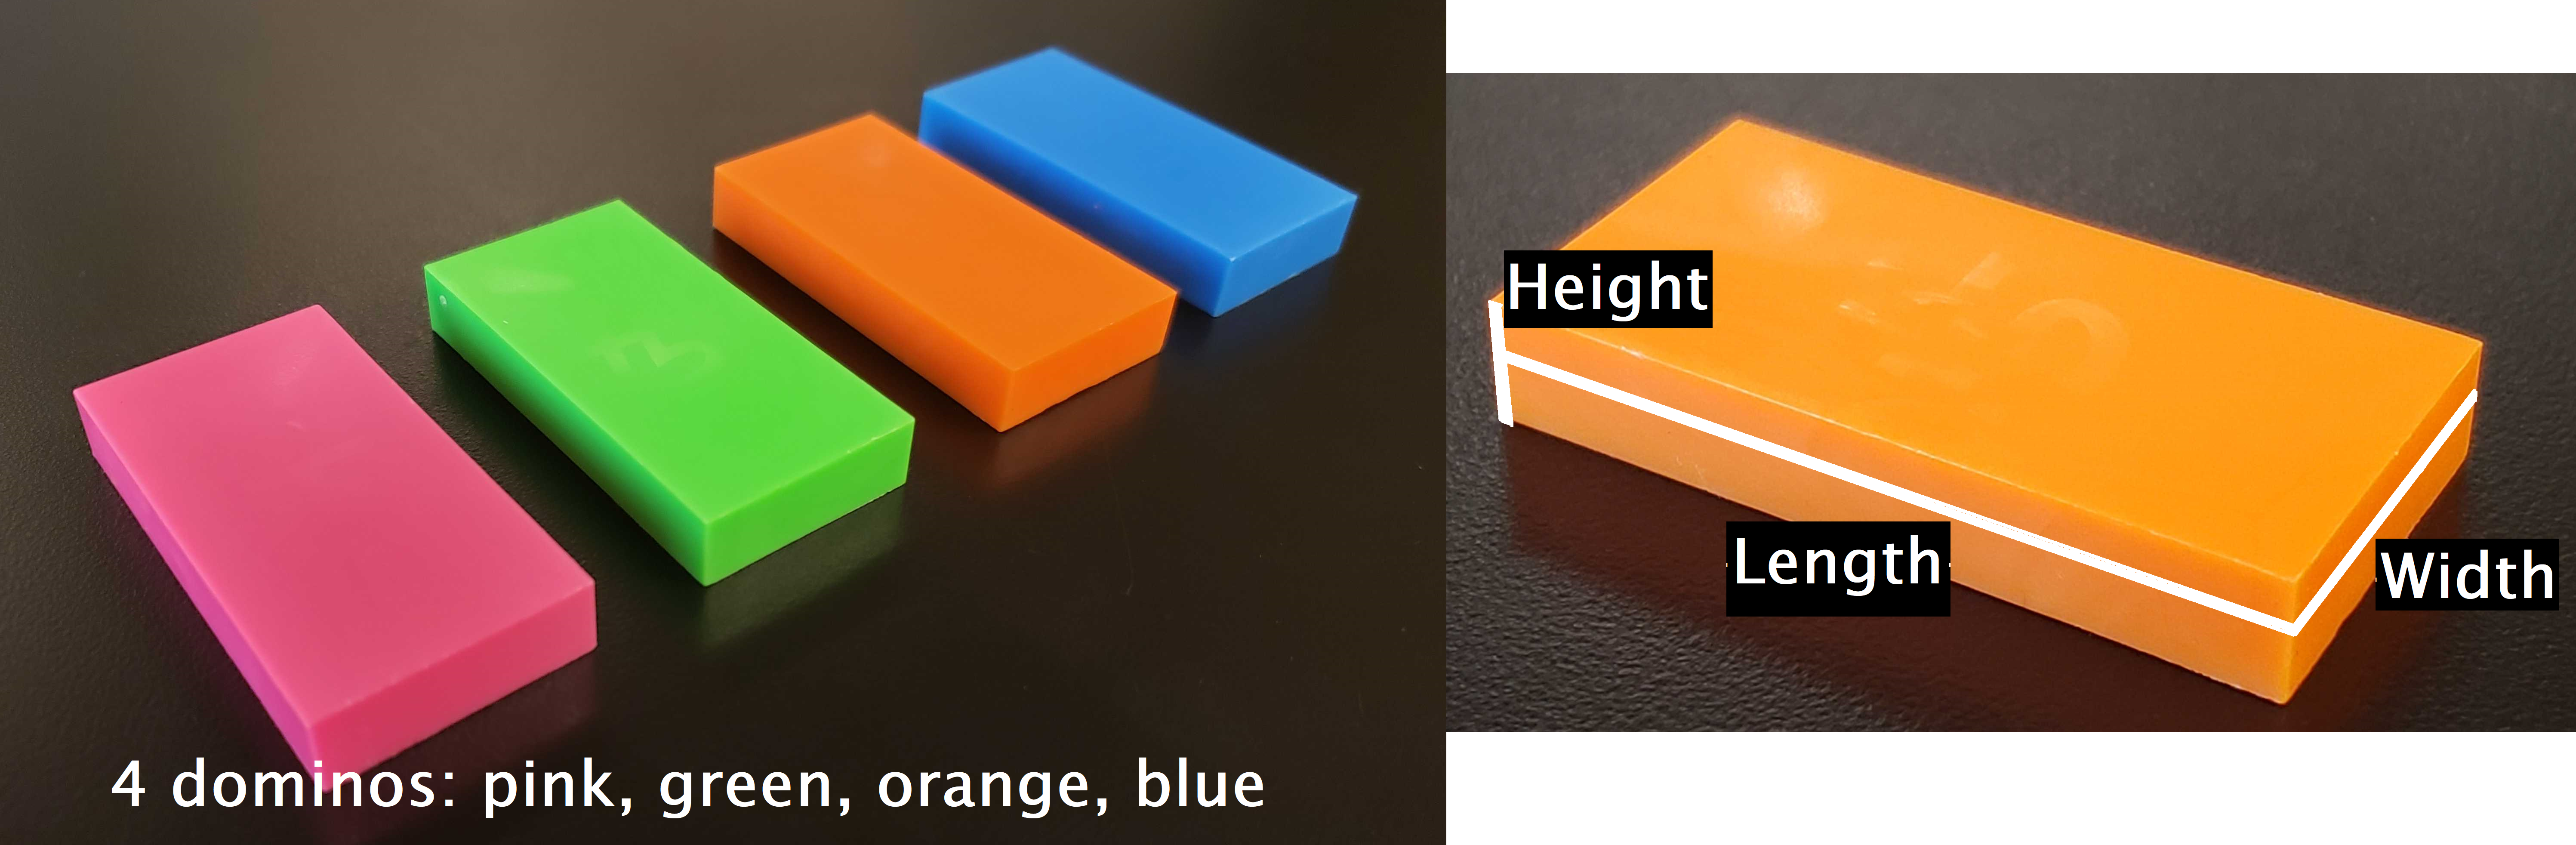
\includegraphics[width=4.9in]{Fall/Experiment00Figures/M0_dominos.png}
  \end{center}
  \caption{Left) Dominoes provided. Right) Relevant length, width, height dimensions of the dominoes.}
  \label{M00Fig01}
\end{figure}

\begin{enumerate}

\item \textbf{OVERALL GOALS:} 
\begin{itemize}
    \item[$\triangleright$] Understand how to take length and mass measurements.
    \item[$\triangleright$] Understand how to characterize measurement uncertainties with standard deviation.
    \item[$\triangleright$] Understand how to characterize measurement uncertainties due to instrument precision.
    \item[$\triangleright$] Each member of the lab group will independently measure the mass, length, width, and height of four provided dominoes per group (i.e. each group gets a pink, green, orange, and blue domino).
\end{itemize}

\textit{NOTE:} It is good practice to \textbf{complete the analysis of trials as you do the experiment}. If there is some error in your experimental method or in your calculation, you can correct it before completing all the other trials. The formulas of the rows for later trials can be created by copying the first trial.

The density of the dominoes' plastic and water are roughly the same. Estimate the value you expect in SI units ($\kilogram/\meter^{3}$). 

\begin{itemize}
	\item[$\triangleright$] Create a Common Data Table for values used in all the trials. In this case, include the instrumental tolerance of the lab scale and the Vernier caliper. 
	\item[$\triangleright$] Create a row for each domino trial. A trial is the measurement by one lab group member of one domino color.
	\item[$\triangleright$] Create a Data Table with columns for:
		\begin{itemize}
			\item Initials of the experimenter
			\item Color of the domino
			\item Measured length $l$, width $w$, height $h$ measured with Vernier calipers and mass $m$ measured with the triple-beam balance in the instruments' units (e.g. mm, $\gram$, etc.)
            \item $l$, $w$, $h$, and $m$ converted to SI units
			\item Calculated volume $V_\text{color}$ for the trial in SI units
			\item Calculated density $\rho_\text{color}$ for the trial in SI units
		\end{itemize}
\end{itemize}

Create a Data Analysis table including:  
\begin{itemize}
    \item Analysis Table 1:
    \begin{itemize}
    	\item[$\triangleright$] Average and standard deviation of the $l_\text{avg.}$length, width, height, volume, and density of each color of domino. 
	   \item[$\triangleright$] Maximum and minimum values of the density and volume based on your experimental value and the instrumental tolerance (i.e. $\pm$ values). \textbf{NOTE:} To maximize Volume $V$, maximize $l$, $w$, $h$. To maximize density $\rho$, maximize $V$ and minimize $m$.
    \end{itemize}
    \item Analysis Table 2:
    \begin{itemize}
        \item[$\triangleright$] Average of the length, width, height, volume, and density of the color set measured by each lab group member.  
    \end{itemize}
\end{itemize}

\end{enumerate}

\pagebreak

\section{Post-Lab Submission --- Interpretation of Results}

\begin{itemize}
    \item[$\triangleright$] Make sure to submit your finalized data table (Excel sheet).
	\item[$\triangleright$] Discuss: Are the densities of all the different colored dominoes the same (within experimental uncertainty based on measurement uncertainties)? Example, do all the $\rho_{\text{blue-person1}}$, $\rho_{\text{blue-person2}}$, etc. agree?
	\item[$\triangleright$] Discuss: Are the average densities of all four dominoes as measured by each person consistent (within experimental uncertainty based on measurement uncertainties)? Example, do all the $\rho_{\text{blue-person1}}$, $\rho_{\text{green-person1}}$, etc. agree?
	\item[$\triangleright$] Discuss: Do you expect the dominoes to float in water (at room temperature)?
    \item[$\triangleright$] What was the precision of your equipment (calipers, triple-beam balance, etc.)?
    \item[$\triangleright$] What are possible systematic errors of the experiment?
\end{itemize}


%\newpage
%\text{ }
%%%%%%%%%%%%%%%%%%%%
%                 File Experiment01.tex        %
%                 Experiment M-1               %
%                   Force Table                %
%                                              %
%%%%%%%%%%%%%%%%%%%%

\labChapter{M}{Force Table with 3 Vectors at Equilibrium}
\label{lab:M1}

% Introduction
%\section{Introduction}
















\section{Background}

\textbf{OVERALL GOALS:}
Use a ``force table" to study:
\begin{enumerate}
\item[$\triangleright$] how vectors are added
\item[$\triangleright$] the concept of force vectors in equilibrium
\end{enumerate}


There are two types of physical quantities: \textbf{\textit{scalars}} and \textbf{\textit{vectors}}. The number of attributes required to define a scalar and a vector distinguishes them. A \textbf{\textit{scalar}} has just a \textbf{magnitude} telling us how large or small something is (or positive or negative); an example of a scalar quantity is temperature or speed ($\meter\per\second$)

A \textbf{\textit{vector}}, meanwhile, is a quantity that is described by both a \textbf{magnitude} \textbf{\textit{and}} \textbf{direction}. Examples of vectors are velocity (speed but with a direction; $\meter\per\second$ at some angle) or force (a push or pull on an object with a specific magnitude at some direction).

A force example: a force may be $100\,\newton$ in magnitude with direction $90\degree$ counterclockwise from the $x$-axis. This force vector is written as $100\,\newton \ @ \ 90\degree$. We will use bold face type to indicate a vector ($\vec{F_i}$) while the regular typeface will indicate scalar magnitudes and the components of a vector ($F_i$).

When several vectors act on an object, it is generally desirable to determine the sum of these vectors, called the \textbf{resultant vector}. Suppose force vectors $\vec{F}_1$ and $\vec{F}_2$ act on a body. The resultant $\vec{R}$ is defined by the vector sum of the two forces, thus
\begin{equation}
   \vec{R} = \vec{F}_1 + \vec{F}_2.
\end{equation}
If many forces act on the body, then we sum all the forces together
\begin{equation}
  \vec{R} = \sum_{i=1}^N \vec{F}_i.
\end{equation}
The resultant force is a single force which can completely represent a number of individual forces acting.  When the resultant force is zero, the object is said to be in equilibrium.

\pagebreak

There are two methods of vector addition to consider:
\begin{enumerate}
\item[$\triangleright$] The graphical method (reviewed here, but not conducted during lab today)
\item[$\triangleright$] The method of components (conducted during lab today)
\end{enumerate}

\subsection{Graphical Method}

Vectors $\vec{F}_1$ and $\vec{F}_2$  (Fig.~\ref{M01Fig01}) are added graphically as follows:
Beginning at a convenient point on a piece of graph paper, usually at the origin of a rectangular coordinate system draw one of the vectors as an arrow to scale and pointing in the proper direction.  Place the second vector with its tail at the tip of the first, again drawn to scale and pointing in the proper direction.  The resultant $\vec{R}$ is the vector drawn from the tail of the first vector to the tip of the second.  The process is illustrated in Fig.~\ref{M01Fig02} demonstrating the addition operation does not depend on the order of addition.  Thus, like scalar addition,
\begin{equation}
  \vec{F}_1 + \vec{F}_2 = \vec{F}_2 + \vec{F}_1 = \vec{R}.
\end{equation}

%Figure01
\begin{figure}[ht]
  \begin{center}        
    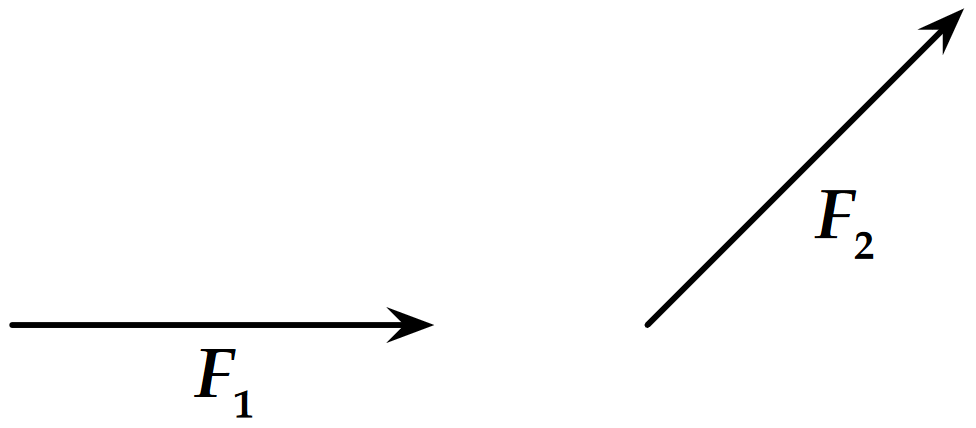
\includegraphics[width=2.2in]{Fall/Experiment01Figures/M1_ForceTable_01.png}
  \end{center}
  \caption{Two force vectors $\vec{F}_1$ and $\vec{F}_2$}
  \label{M01Fig01}  % the \label command comes AFTER the caption
\end{figure}


%Figure02
\begin{figure}%[ht]
  \begin{center}
    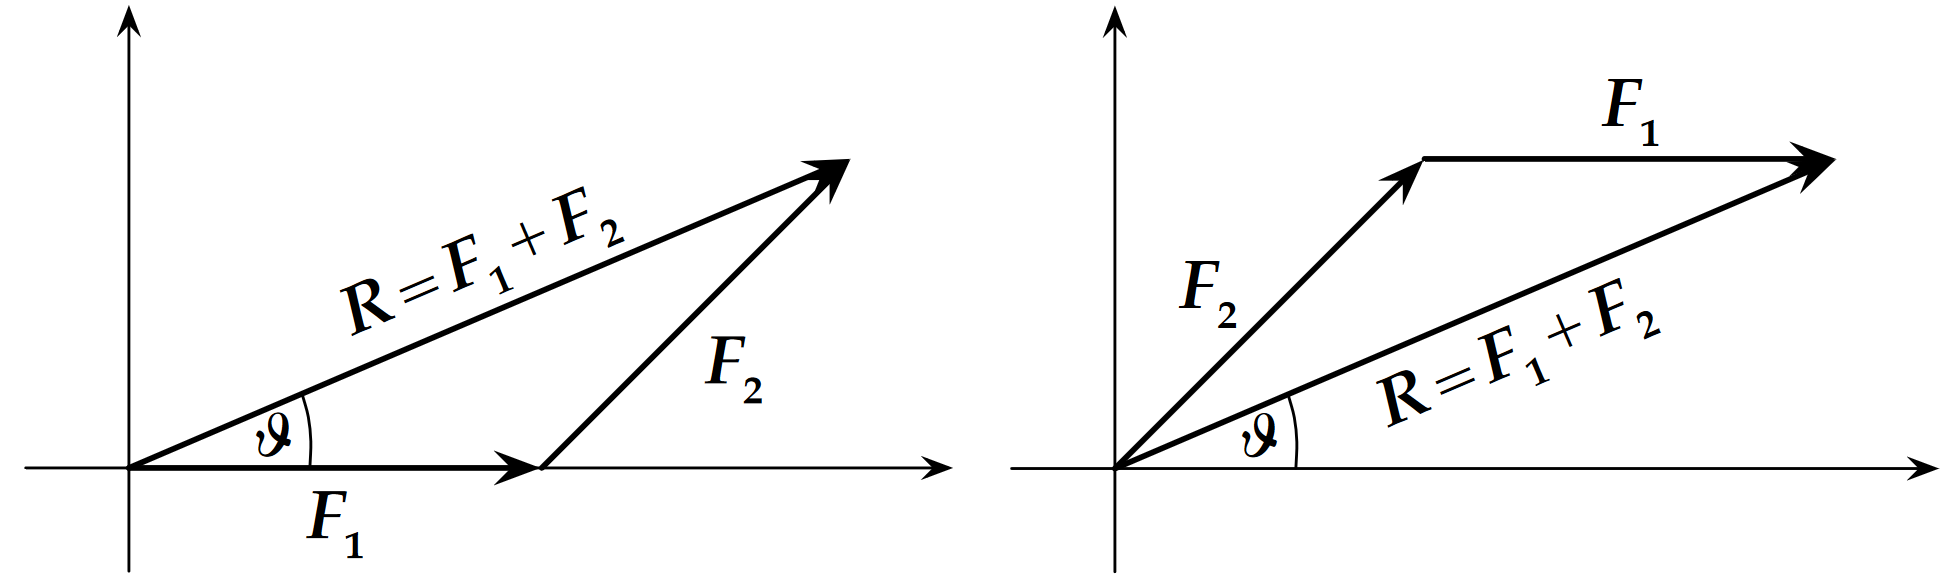
\includegraphics[width=5.6in]{Experiment01Figures/M1_ForceTable_02.png}
  \end{center}
  \caption{Adding 2 vectors $\vec{F}_1$ and $\vec{F}_2$, using the graphical (``tail-to-tip'') method.}
  \label{M01Fig02}
\end{figure}

It is important that an appropriate scale be selected with which the vectors are drawn (e.g.\ $1\,\newton = 10\,\centi\meter$). The magnitude of $\vec{R}$ is determined using a ruler, and the angle $\theta$ is measured using a protractor.  Since the negative of a vector is merely the vector pointing in the opposite direction, subtraction is addition with the negative vector pointing in the opposite direction.  Errors can be significantly reduced by using a scale that makes the drawing as large as possible. Neatness counts!

% Method of Components
\subsection{Method of Components}

The method of components is a much more useful and quantitatively accurate method of vector addition.  Each vector is resolved into components along the $x-$ and $y$-axes. That is to say, the vector addition of the two components of the vector is the vector itself.  Thus if two vectors are to be added, we add the components along each axis to form the components of the resultant.

%Figure03
\begin{figure}[ht]
  \begin{center}
    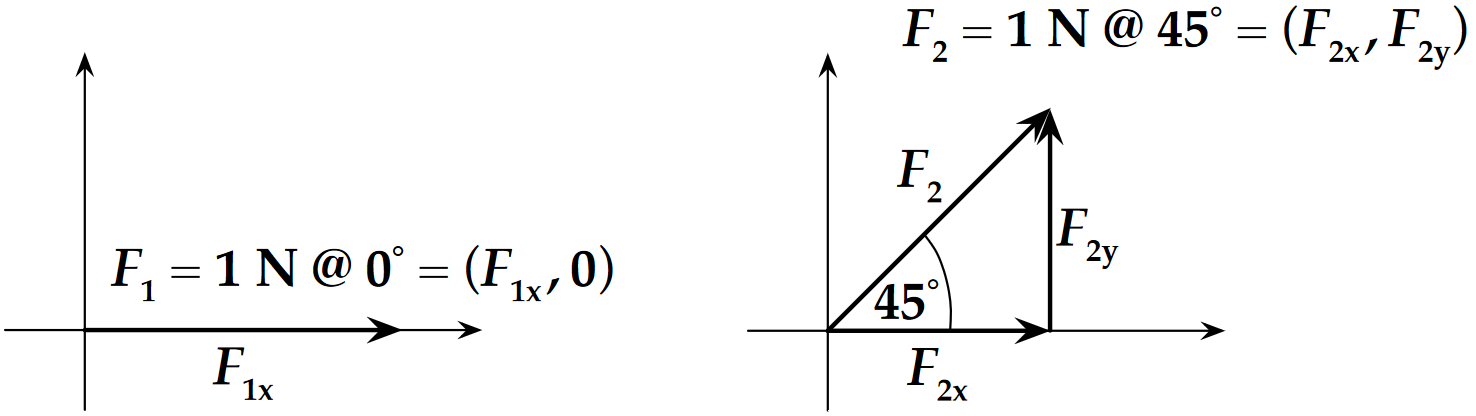
\includegraphics[width=5.6in]{Fall/Experiment01Figures/M1_ForceTable_03.png}
  \end{center}
  \caption{Adding 2 vectors $\vec{F}_1$ and $\vec{F}_2$ using the method of components. }
  \label{M01Fig03}
\end{figure}

In Fig.~\ref{M01Fig03}, the magnitudes and directions are shown for the two force vectors $\vec{F}_1$ and $\vec{F}_2$ . The magnitudes of the $x$ and $y$ components are calculated for this example as follows:
\begin{equation}
\label{Eq:M1_cosSinAngle}
  \begin{aligned} %
    F_{1,x} & = F_1 \, \cos(\theta_{1}) & \qquad F_{2,x} & = F_2 \, \cos(\theta_{2}) \\
            & = 1\,\newton\ \cos(0\degree) = 1\,\newton & &  = 1\,\newton\ \cos(45\degree) = 0.707\,\newton \\
    F_{1,y} & = F_1 \,\sin(\theta_1) & \qquad F_{2,y} & = F_2 \,\sin(\theta_2) \\
            & = 1\,\newton\ \sin(0\degree) = 0\,\newton & &  = 1\,\newton\ \sin(45\degree) = 0.707\,\newton.
  \end{aligned}
\end{equation}
Next, add the $x$-components
\[
  \vec{R}_x = F_{1,x} + F_{2,x} = 1\,\newton + 0.707\,\newton = 1.707\,\newton.
\]
Then, add the $y$-components
\[
  \vec{R}_y = F_{1,y} + F_{2,y} = 0\,\newton + 0.707\,\newton = 0.707\,\newton.
\]
The magnitude of the resultant is found using the relation
\begin{equation}
\label{Eq:M1_resultantMag}
	\vec{R}^2 = {\vec{R}_x}^2 + {\vec{R}_y}^2,
\end{equation}
or
\[
  \vec{R} = \sqrt{\left(1.707\,\newton\right)^2 +
    \left(0.707\,\newton\right)^2} = 1.848\,\newton.
\]
The angle $\theta$ specifies the direction of the resultant and it can be calculated by noting that
\begin{equation}
  \tan\theta = R_{y} / R_{x}
\end{equation}
and
\begin{align} %
\label{Eq:M1_arctan}
  \theta = \arctan (R_{y} / R_{x}).
\end{align}

For this example illustrated in Fig.~\ref{M01Fig04}
\begin{align} %
  \tan \theta = (0.707\,\newton) / (1.707\,\newton) = 0.414\,\newton,
\end{align}
\begin{align} %
  \theta = \arctan(0.414) = 22.5\degree.
\end{align}

%Figure04
\begin{figure}[h]
  \begin{center}
    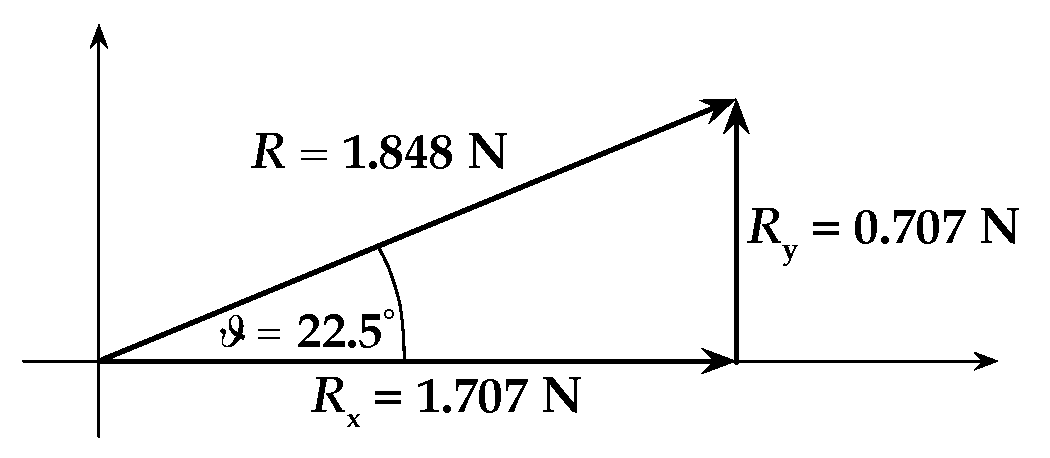
\includegraphics[width=3.5in]{Experiment01Figures/Figure04.pdf}
  \end{center}
  \caption{Example of $\vec{R}$, the sum of 2 vectors, illustrating $x$- and $y$-components, a well as its magnitude and angle with the $x$-axis.}
  \label{M01Fig04} 
\end{figure}



In this laboratory, an object will be presented with two known forces acting on it.  Equilibrium will be established by adding a third \textbf{equilibrant} force $\vec{F}_3$, such that the sum of the three forces is zero (at equilibrium). Thus, we must find the resultant $\vec{R}$ of the two given forces $\vec{F}_1$ and $\vec{F}_2$, and find the force $\vec{F}_3 = -\vec{R}$ --- equal in magnitude and opposite in direction to the resultant $\vec{R}$ of $\vec{F}_1$ and $\vec{F}_2$.  This is illustrated in Fig.~\ref{M01Fig05}.


%Figure05
\begin{figure}[h]
  \begin{center}
    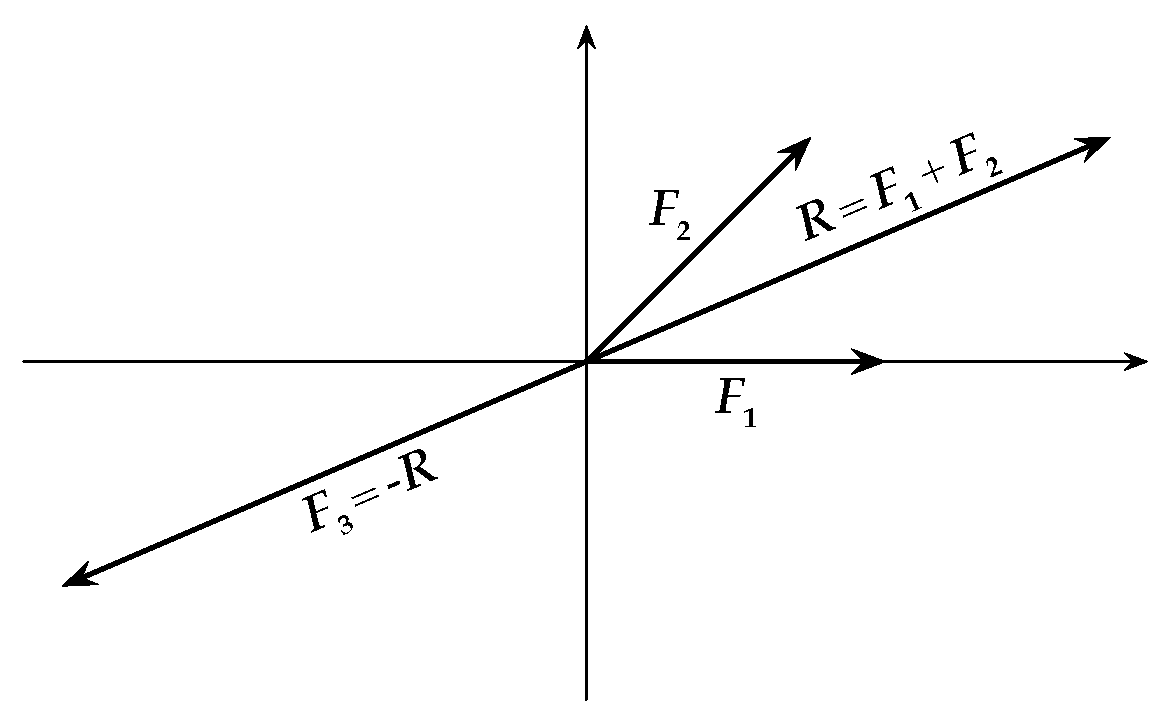
\includegraphics[width=3.6in]{Experiment01Figures/Figure05.pdf}
  \end{center}
  \caption{Illustration of the method to determine the force $\vec{F}_{3}$ needed to balance two given forces $\vec{F}_{1}$ and $\vec{F}_{2}$.}
  \label{M01Fig05}
\end{figure}

Here $\vec{F}_3$ is the equilibrant force necessary to equilibrate $\vec{F}_1$ and $\vec{F}_2$.  Note that, the resultant of $\vec{F}_1+\vec{F}_2+\vec{F}_3$ is zero since the ring is in equilibrium.

Force $\vec{F}_3$ has the same magnitude as the resultant $\vec{R}$, but acts in a direction opposite to $\vec{R}$ (recall that $\vec{R}=\vec{F}_1+\vec{F}_2$).  So we now have
\begin{equation}
  \vec{F}_3 = -\vec{R}.
\end{equation}
We conclude that the force necessary to equilibrate two or more forces is equal and opposite to the resultant of the two (or more) forces. This is additionally illustrated in an example of the force table apparatus we will use in Fig.~\ref{M01Fig06} right.





\underline{\textbf{Apparatus}}


%Figure05
\begin{figure}[h]
  \begin{center}
    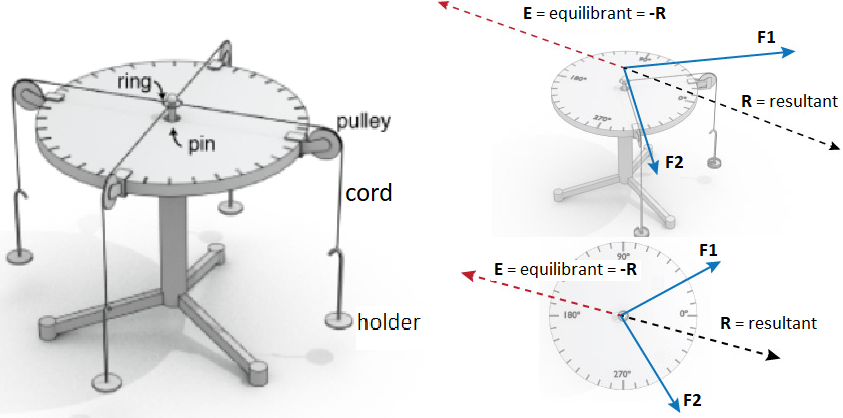
\includegraphics[width=5.5in]{Fall/Experiment01Figures/M1_ForceTable_06_table.png}
  \end{center}
  \caption{Illustration of the force table, and an example of to determine the force $\vec{F}_{3}$ needed to balance two given forces $\vec{F}_{1}$ and $\vec{F}_{2}$.}
  \label{M01Fig06}
\end{figure}

The apparatus for this experiment consist of a force table, weight holders, and weights (see Fig.~\ref{M01Fig06}).  The force table consists of a circular tabletop mounted on a vertical rod held in a tripod support with leveling screws.  The rim of the circular top has a $360\degree$ scale engraved on it along which it is possible to clamp a number of pulleys.  At the center of the table is a small ring held in place by means of a removable pin.  The ends of three cords are tied to the ring with each cord leading over a pulley and ending with a weight holder tied to its other end. When the forces along the cords acting upon the small ring are balanced, or in static equilibrium, the ring remains stationary. For this lab, the force pulling on the ring is the tension of the string, which is merely translated from horizontal on the table to vertical 


Each hanging mass has an associated weight (force) due to being pulled \textit{down} by gravity. This weight is balanced by the \textit{upward }tension force of the vertical part of the cord which is merely translated from vertical to horizontal tension by the pulley. Thus, the force pulling the ring in the direction of the cord is

\begin{equation}
  \label{eq:M01_ForceG}
  \vec{F_\text{weight}} = m \times \vec{g} = \vec{F_\text{tension}}
\end{equation}


For accurate measurements of the angles involved, each cord must be aimed directly at the center of the ring requiring that the equilibrium condition must be established when the ring is exactly centered around the pin on the table.



\section{Experimental Procedure}

\subsection{Preview}

For today's lab, two different cases will be assigned involving two given vectors and the \textbf{determination of the equilibrant vector}. A third case involves the \textbf{determination of the mass of two unlabeled masses} by balancing the system from a single known mass.% and changing the angles such that the angles are then assumed to be actual or true values (no uncertainty) system is balanced are the accepted values.

\underline{\textbf{Finding the Equilibrant (First two cases)}}


For each of the first two cases, you will have two given masses at given angles (direction).  Each mass, consisting of a $50\,\gram$ hanger plus the necessary additional mass, will be hung from a cord routed over a pulley at the assigned angular positions and finally tied to the ring.  A third cord, hanger, and pulley assembly is put in place for the third, unknown force vector.  Each force is the weight of the hanging mass at the pulley angle.  Determine the unknown forces for each of the two cases. % After you determine the unknown force in the third case, tilt the force table and determine any change in the third force with the tilted table.

If, for example, you are given the following case to work with
\[
\begin{array}{rll}
  \mbox{Mass \#1:} & 200\,\gram & \mbox{@}\,0\degree \\
  \mbox{Mass \#2:} & 250\,\gram & \mbox{@}\,135\degree.
\end{array}
\]
Place a pulley at $0\degree$ and add $150\,\gram$ to the $50\,\gram$ weight hanger for a total $200\,\gram$.  As mentioned in Eqn.~\ref{eq:M01_ForceG}, the tension on the cord is the same on both sides of the pulley so that the downward pull of gravity on the hanger and masses is equal to the tension in the cord leading to the ring.  Thus,
\[
\vec{F}_1 = m g = 0.20\,\kilo\gram\times 9.8\,\meter\per\second\squared
         = 1.96\,\newton\ @\ 0\degree.
\]
Similarly, add $200\,\gram$ to a $50\,\gram$ weight hanger and run its cord over a pulley mounted at $135\degree$.
\[
\vec{F}_2 = m g = 0.25\,\kilo\gram\times 9.8\,\metre\per\second\squared
         = 2.45\,\newton\ @ \ 135\degree.
\]

Having established the given magnitudes and directions for each of the given forces, $\vec{F}_{1}$ and $\vec{F}_{2}$, adjust both the amount of mass hanging on cord 3 and its angular position so that the ring is stationary at the center of the table.  In order for angular measurements to be accurate, \textbf{each cord must be on a line that crosses through the center of the table}.  Sighting \textit{along} each cord towards the center pin can help you to easily and accurately check this.

To determine the equilibrant vector $\vec{F}_{3}$, you will record both the angular position (\textbf{direction}) and total mass (to determine \textbf{magnitude} of the balancing force from the total hanging weight) required to balance $\vec{F}_{1}$ and $\vec{F}_{2}$.


\underline{\textbf{Determining 2 Unlabeled Masses (Third case)}}


In this case, you will experimentally \textbf{determine two unlabeled masses} by balancing the $x$ and $y$ components of the force of a known mass.
Place the pulley with the known mass $M_1 = 50\,\gram $ at $\theta_1 = 0\degree$.
Experimentally determine the angles $\theta_2$ and $\theta_3$ for the unlabeled masses $M_2$ and $M_3$ that result in the ring being in equilibrium. For this case, \textbf{assume angles $\theta_2$ and $\theta_3$ are actual values}.

%First find $M_2$ and $M_3$ using the graphical method.
%Accurately draw $ \vec{F}_1$ on graph paper using an appropriate scale.
%Draw a line in the direction of $\vec{F}_2$ at angle $\theta_2$ through the head of $\vec{F}_1$.
%Draw a line in the direction of $\vec{F}_3$ at angle $\theta_3$ through the tail of $\vec{F}_1$.
%Find the point where these two lines intersect to form a triangle representing equilibrium of the three forces.
%Determine the magnitude of $\vec{F}_2$ and $\vec{F}_3$ using your selected scale by measuring the sides of the triangle.
%Find the unknown masses by dividing by $g$.

We can calculate the theoretical unlabeled masses using the method of components.
You have to solve a pair of equations for the $x$ and $y$ components of force.
%This calculation is the algebraic version of finding the intersection of the two lines in the graphical method.
The equation for equilibrium in the $x$ direction is
\begin{equation}
  \label{eq:M01unknownx}
  (M_1 + M_2 \cos\theta_2 + M_3 \cos\theta_3)g = 0.
\end{equation}
The equation for equilibrium in the $y$ direction is
\begin{equation}
  \label{eq:M01unknowny}
  (M_2 \sin\theta_2 + M_3 \sin\theta_3)g = 0.
\end{equation}
$M_2$ is eliminated by multiplying the $x$ component by $\sin \theta_2$ and subtracting the $y$ component multiplied by $\cos \theta_2$
\begin{equation}
  \label{eq:M01solveM3}
  M_1 \sin \theta_2  + M_3 \cos \theta_3 \sin \theta_2 - M_3 \sin \theta_3 \cos \theta_2 = 0.
\end{equation}
Using the known values, solve for $M_3$ and enter the value in the table.

Similarly, eliminating $M_3$ gives
\begin{equation}
  \label{eq:M01solveM2}
  M_1 \sin \theta_3  + M_2 \cos \theta_2 \sin \theta_3 - M_2 \sin \theta_2 \cos \theta_3 = 0.
\end{equation}
Using the known values, solve for $M_2$ and enter the value in the table.

Measure $M_2$ and $M_3$ on the scale and enter the values in the table.










%Data analysis includes estimated or calculated errors. See the guidance starting at page \ref{sec:TypesErrors}.

It is good practice to \textbf{COMPLETE THE ANALYSIS OF THE FIRST CASE BEFORE CONTINUING TO THE NEXT CASE}. If you have some error in your experimental method or in your calculation, you can correct it before completing all the other cases. The layout of the data table for additional cases can then be created by copying the first case after you are confident in your results from the first case.


\subsection{CASE 1 \& 2 -- Finding the Equilibrant Vector (Balancing Force)}

\begin{enumerate}
\item \textbf{OVERALL GOALS:} 
\begin{itemize}
    \item Understand how to add and balance vectors using the \textbf{method of components}.
    \item Conduct 3 cases of two additive, known vectors (weights at given angles) to experimentally determine the third balancing or equilibrant vector.
    \item Compare the experimental results to theoretically expected vectors.
    \item \textbf{Assume} $0\degree$ is the $+x$ direction, $90 \degree$ is the $+y$ direction
\end{itemize}

\pagebreak

\item The first two cases are:
   % \begin{itemize}
  %      \item Case 1: 
  %      \begin{itemize}
  %          \item hanger 1: 150 g @ 0$\degree$
  %          \item hanger 2: 150 g @ 70$\degree$
  %          \item hanger 3: ? kg @ ?$\degree$
  %      \end{itemize}
  %      \item Case 2: 
  %      \begin{itemize}
  %          \item hanger 1: 100 g @ 75$\degree$
  %          \item hanger 2: 200 g @ 115$\degree$
  %          \item hanger 3: ? kg @ ?$\degree$
  %      \end{itemize}
  %      \item Case 3: 
  %      \begin{itemize}
  %          \item hanger 1: 150 g @ 120$\degree$
  %          \item hanger 2: 250 g @ 200$\degree$
  %          \item hanger 3: ? kg @ ?$\degree$
  %      \end{itemize}
  %  \end{itemize}

    \begin{tabular}{l|l}
    \textbf{Case 1:}     &  \hspace{20mm} \textbf{Case 2:} \\
    --- hanger 1: 150 g @ 0$\degree$    \hspace{20mm} & \hspace{20mm} --- hanger 1: 100 g @ 75$\degree$ \\
    --- hanger 2: 150 g @ 70$\degree$     & \hspace{20mm} --- hanger 2: 200 g @ 115$\degree$ \\
    --- hanger 3: ? kg @ ?$\degree$     & \hspace{20mm} --- hanger 3: ? kg @ ?$\degree$
    \end{tabular}

\item Create a data table for the first case. NOTE: The data layout for each of the first two cases is the same. Create for the first case and run the whole experiment, then you can copy/paste the same data table for the additional case(s).
%\item 
\begin{itemize}
    \item Common data section with accepted value of $g$ ($9.803\,\meter\per\second\squared$), mass of the hanger, and any other common values. You will reference these values in the calculations.
    \item With \textbf{three rows} (1 for each of the 3 vectors).% Also include additional \textbf{rows} for the average $g$ value, the $\pm$ uncertainty in gravity $\delta g$, the magnitude difference compared to the accepted $g$, \% diff. compared to the accepted $g$ \textit{DISCUSSION POINT for later}: How well does you average value of $g \pm \delta g$ agree with the accepted value of $g$?).
    \item Include \textbf{columns} for:
    \begin{itemize}
        \item $m_i$: hanging mass in kilograms (\kilo\gram)
        \item $\delta m_i$: your estimate of the experimental uncertainty [$\pm$ value] of the mass
        \item $F_i$: calculated magnitude of the force in Newtons (N) (see Eqn.~\ref{eq:M01_ForceG})
%        \item $\delta \vec{F}_i$: your derived experimental uncertainty of the magnitude of the force (e.g. $\delta \vec{F}_i = ((m_i + \delta m_i) \times \vec{g}) - ((m_i) \times \vec{g})$) where you are trying to make the final force value (due to $m_i + \delta m_i$) as large as possible to find the widest range of propagated uncertainty for a derived value
        \item $\theta_i$: direction of the force vector in degrees
        \item $\delta \theta_i$: your estimate of the experimental uncertainty of the angle
        \item $F_{i,x}$: calculated $x$-component of the force vectors (see Eqn.~\ref{Eq:M1_cosSinAngle}). Reminder, Excel needs angles in radians (use RADIANS() function to convert)
        %\item $\delta \vec{F}_x$: your derived uncertainty of the $x$-component, again trying to maximize the magnitude of the uncertainty (e.g $\delta \vec{F}_x = (\vec{F}_i + \delta \vec{F}_i) \times \cos{(\theta \pm \delta \theta)}$)
        \item $F_{i,y}$: calculated $y$-component of the force vectors
        %\item $\delta \vec{F}_y$: your derived uncertainty of the $y$-component in a similar manner (e.g $\delta \vec{F}_y = (\vec{F}_i + \delta \vec{F}_i) \times \sin{(\theta \pm \delta \theta)}$)
    \end{itemize} 
    \item Create a secondary table to analyze the results of your measurements. This is effectively one row as there would be just a single value for each of the variables. The columns should include variables:
     \begin{itemize}
        \item $\vec{R}_x$ \& $\vec{R}_y$: the $x$ and $y$ components of the resultant vector $\vec{R}$ of the two given force vectors $\vec{F}_1$ and $\vec{F}_2$
        \item $\vec{R}_\text{mag}$: magnitude of the resultant force vector in Newtons (see Pythagorean Theorem in Eqn.~\ref{Eq:M1_resultantMag})
        \item $\theta_{R}$: direction of the resultant in degrees (see Eqn.~\ref{Eq:M1_arctan} which stems from trigonometry). Use ATAN2() Excel function to get angle as measured counterclockwise from $0\degree$. Reminder, Excel returns angles in radians (use DEGREES() function to convert)

        \item $\vec{F}_{x,\text{total experimental}}$ \& $\vec{F}_{y,\text{total experimental}}$: the vector components of the measured total force, which is the vector sum of $\vec{R}$ and $\vec{F}_3$

        \item $\vec{F}_{mag,\text{total experimental}}$ (a.k.a. $\delta \vec{F}_3$): the magnitude of the total force, determined in similar fashion to Eqn.~\ref{Eq:M1_resultantMag}, but with $\vec{F}_{x,\text{total experimental}}$ \& \newline $\vec{F}_{y,\text{total experimental}}$. \textit{\textbf{Consider}}: The \textbf{total force should be zero} because the ring is in equilibrium. The magnitude of the total force is therefore a measure of the \textit{experimental uncertainty}. This effectively represents $\delta \vec{F}_3$ where your experimental result would be $\vec{F}_3 \pm \delta \vec{F}_3$.

        
        \item Based on your determined resultant $\vec{R}$
            \begin{itemize}
                \item $\vec{F}_{3,\text{theoretical}}$: your expected or theoretical magnitude of the equilibrant force in N
                \item $m_3,\text{theoretical}$: theoretical equilibrant mass in kg
%                \item $\delta m_{3,\text{theoretical}}$: uncertainty of $m_3,\text{theoretical}$ in kg as derived from 
                \item $\theta_{3,\text{theoretical}}$: theoretical equilibrant direction in deg. (e.g. $\theta_{R} + 180 \degree$)
            \end{itemize}
        
     


%        \item \% Difference between experimental Equilibrant force and theoretical
%        \item \% Difference between experimental Equilibrant direction and theoretical
    \end{itemize} 
\end{itemize}


    \item Starting with the first case, place the respective masses on hangers 1 \& 2
    \item Unscrew the black pulleys to rotate them around the tabletop to their given angles
    \item With hanger 3, add or subtract masses and scoot the pulley around the table until the ring is as perfectly centered around the center pin as possible to argue equilibrium
    \item Note your $m_3$ \& $\theta_3$ values. Also note your estimated uncertainties $\delta m_i$ \& $\delta \theta_i$
    \item Derive the hangers' respective forces (e.g. Eqn~\ref{eq:M01_ForceG})
    \item Determine the hangers' respective $x$ and $y$ components
    \item Determine the resultant $\vec{R}$ from your derived values for $\vec{R}_x$, $\vec{R}_y$
    \item Determine the resultant's angle $\theta_R$
    \item COMPARE your experimental results of hanger 3 to the theoretical values. Does $\vec{F}_3 \pm \delta \vec{F}_3$ overlap (and therefore agree) with your theoretical value $\vec{F}_{3,\text{theoretical}}$? If not, are there significant issues that may be contributing to the discrepancy? Discuss with instructor if so. To be further discussed in Sec.~\ref{M1:Interpretation}
    \item Repeat for the second case
\end{enumerate}





\subsection{CASE 3 -- Determining 2 Unlabeled Masses}




\begin{enumerate}
\item \textbf{OVERALL GOALS:} 
\begin{itemize}
    \item Understand how to determine two unknown values of a 3 vector system using the \textbf{method of components}. 
    \item \textit{CONSIDER}: Each vector has two pieces of information, \textbf{magnitude} and \textbf{direction} --- how many pieces of information total do we have to work from?
    \item Determine the masses of two figurines (one is a black Pikachu, the other is a white corgi that can each sit on their respective hangers) by balancing the force vectors. Treat Pikachu-black as $m_2$ and the corgi-white as $m_3$.
    \item Compare the experimental results to actual masses as measured with a triple-beam balance.
    \item \textbf{Assume} the angles for both Pikachu and the corgi, once found, are treated as given values (so you only have two unknowns with two equations).
\end{itemize}

\item The third case is:
    \begin{itemize}
        \item hanger 1: \space\space\space\space\space\space\space\space\space\space\space\space\space\space\space\space\space50 g @ 0$\degree$
        \item hanger 2 (Pikachu-black): ? kg @ ?$\degree$ (angle treated as given once determined)
        \item hanger 3 (corgi-white): \space\space\space? kg @ ?$\degree$ (angle treated as given once determined)
    \end{itemize}

\item Create a data table for this case:
\begin{itemize}
    \item Common data section with the accepted value of $g$ ($9.803\,\meter\per\second\squared$), the mass of the hanger, actual values of the figurines to be determined later, and any other common values.
    \item $m_1$: Given mass will be just the hanger, so 50 $\gram$ (but record in \kilo\gram)
    \item $\theta_1$: Angle of 0\degree for the empty hanger
    \item $\vec{F}_{x,1}$ \& $\vec{F}_{y,1}$: $x$ and $y$ components of the known mass's force vector
    \item $\theta_{2,\text{Pikachu-black}}$ \& $\theta_{3,\text{corgi-white}}$: Experimentally determined direction of the force vector in degrees --- \textbf{treat as actual given values once you find equilibrium. You will use these to solve for the masses later.}
    \item $m_{2,\text{Pikachu-black}}$ \& $m_{3,\text{corgi-white}}$: the experimental values of $m_2$ and $m_3$ from Eqn.~\ref{eq:M01solveM3} and Eqn.~\ref{eq:M01solveM2}
    \item $m_{2,\text{Pikachu-black, actual}}$ \& $m_{3,\text{corgi-white, actual}}$: the values of $m_2$ and $m_3$ as measured on a triple-beam balance.
    \item \% Difference of $m_2$ and $m_3$ experimentally found values to the actual measured values (see Eqn.~\ref{M1:PercentDiff} in Sec.~\ref{M1:Interpretation}).
\end{itemize}



    \item Place the respective masses on there hangers, with $m_1$ set to 0\degree
    \item Unscrew the black pulleys to rotate them around the tabletop until you find equilibrium. You are only changing the angles of $\theta_{2,\text{Pikachu-black}}$ \& $\theta_{3,\text{corgi-white}}$. NO ADDITIONAL MASS IS REQUIRED.
    \item Once you've found equilibrium, note the $\theta_{2,\text{Pikachu-black}}$ \& $\theta_{3,\text{corgi-white}}$ values as actual values to use in later equations (i.e. as if they're given angles)
    \item Determine $m_{2,\text{Pikachu-black}}$ \& $m_{3,\text{corgi-white}}$ using Eqn.~\ref{eq:M01solveM3} and Eqn.~\ref{eq:M01solveM2}
    \item Using a triple-beam balance, measure directly the actual mass of $m_{2,\text{Pikachu-black, actual}}$ \& $m_{3,\text{corgi-white, actual}}$
    \item COMPARE your experimental results of each of the unlabeled masses to their actual values. Calculate the \% difference of $m_2$ and $m_3$ experimentally found values to the actual measured values. What may be contributing to a larger or smaller difference? To be further discussed in Sec.~\ref{M1:Interpretation}.

\end{enumerate}


Post-Lab Submission --- Interpretation of Results on next page $\xrightarrow{}$




\pagebreak

% Interpretation of Results
\section{Post-Lab Submission --- Interpretation of Results}
\label{M1:Interpretation}
\begin{itemize}

\item Make sure to submit your finalized data table (Excel sheet)
\item What is a vector?
\item Case 1 \& 2 (Finding Equilibrant):
\begin{itemize}
    \item Looking at your experiment, why do the two given masses not add up to the third mass?
    \item What are the uncertainties of Experiment 1?
    \item What are your results, and how do they compare to the theoretical predictions?
        \begin{itemize}
        \item In other words, for each of the first two cases, COMPARE your experimental results of hanger 3 to the theoretical values for hanger 3.
            \begin{itemize}
            \item Does $\vec{F}_3 \pm \delta \vec{F}_3$ overlap (and therefore agree) with your theoretical value $\vec{F}_{3,\text{theoretical}}$? 
            \item Does $m_3 \pm \delta m_3$ overlap with your theoretical value $m_{3,\text{theoretical}}$?
            \item Does $\theta_3 \pm \delta \theta_3$ overlap with your theoretical value $\theta_{3,\text{theoretical}}$?
            \end{itemize}
        \end{itemize}
%    \item Does $\vec{F}_{mag,\text{total experimental}}$ actually equal zero?
    \item How does adding a few grams (i.e. $m_3 + \delta m_3$) change your results for $\vec{F}_3$?
    \item How does changing the angle (i.e. $\theta_3 \pm \delta \theta_3$) change your results $\vec{F}_3$?
\end{itemize}

\item Case 3 (Unlabeled Masses):
\begin{itemize}
    \item How do your values for $m_\text{Pikachu-black}$ and $m_\text{corgi-white}$ compare to your actual values from the triple-beam-balance?
    \item What is the percent difference between your experimentally determine masses and their actual measured values? Calculate the \% difference in each of the masses using the following relation:
	\begin{align} %
        \label{M1:PercentDiff}
	\mbox{\% Difference} = \frac{\mbox{Experimental} \ \mbox{Value} - \mbox{Actual} \ \mbox{Value}}{\mbox{Actual} \ \mbox{Value}} \times 100\%.
	\end{align}
    \item What uncertainties might make this difference larger or smaller?
\end{itemize}
\item What is the precision of your equipment (force table, masses, etc.)?
\item What are possible systematic errors of the experiment?




    
%\item[$\triangleright$] Find the resultant force for each of the three experimental cases. Using the method of components, find the magnitude and direction of this resultant $\vec{R}$.  The balancing force $\vec{F}_{3}$ equals the negative of resultant $\vec{R}$ of $ \vec{F}_{1}$ and $\vec{F}_{2}$, i.e.\ the direction of $\vec{F}_{3}$ is $180\degree$ from $\vec{R}$.
%%\item[$\triangleright$] For one of the cases, plot the vectors $\vec{F}_{1}$ and $\vec{F}_{2}$.  Graphically construct and draw the vector $\vec{R}$.  From $\vec{R}$, construct the expected $\vec{F}_{3}$.  On the same graph, plot your experimentally determined vector $\vec{F}_{3}$ and compare the two $\vec{F}_{3}$ vectors.
%          Calculate the \% difference in the magnitudes of the two vectors using the following relation:
%	\begin{align} %
%	\mbox{\% Difference} = \frac{\mbox{Experimental} \ \mbox{Value} - \mbox{Calculated} \ \mbox{Value}}{\mbox{Calculated} \ \mbox{Value}} \times 100\%.
%	\end{align}
%\item[$\triangleright$] Discuss in your lab report any discrepancy in the directions of the two vectors as well as their magnitude.
%%\item[$\triangleright$] Assume the force table is not level while you perform the experiment. Discuss the effect this would have on the outcome of your measurement of the equilibrium force $\vec{F}_{3}$. To determine this, tilt the balanced force table for one of the cases. Discuss the outcome among yourselves and with your lab instructor.
\end{itemize}


\newpage
\text{ }
%%%%%%%%%%%%%%%%%%%%%
%                                          %
%                 Experiment M-2           %
%         Acceleration due to gravity      %
%                                          %
%%%%%%%%%%%%%%%%%%%%%

\labChapter{M}{Acceleration due to Gravity, \textit{g}, with Glider on Tilted Air Track}

\label{lab:M2}

%\section{Introduction}
\section{Background}



By measuring the acceleration of a mass moving under the influence of the gravitational attraction of the earth, namely its weight, we can determine the acceleration due to gravity, usually denoted by $g$.  The mass will be allowed to accelerate down a presumed frictionless, inclined plane.  Measurement of the acceleration along the plane is directly related to the acceleration due to gravity by a simple trigonometric relationship.  The use of the plane permits the convenient measurement of a small, measurable fraction of the acceleration due to gravity.  This of course is in lieu of the much more difficult measurement of a vertically falling mass.














Near the surface of the earth, the attractive force of the earth on a mass can be considered a constant over a reasonable range of elevation. This force is commonly called the weight of the object and from Newton's Second Law the weight is the mass, $m$, times the acceleration due to gravity. Using Fig.~\ref{M02Fig01}. and the derivation following, we can see that the value of $g$ can be easily determined by a few simple measurements.

\begin{figure}
  \begin{center}  
    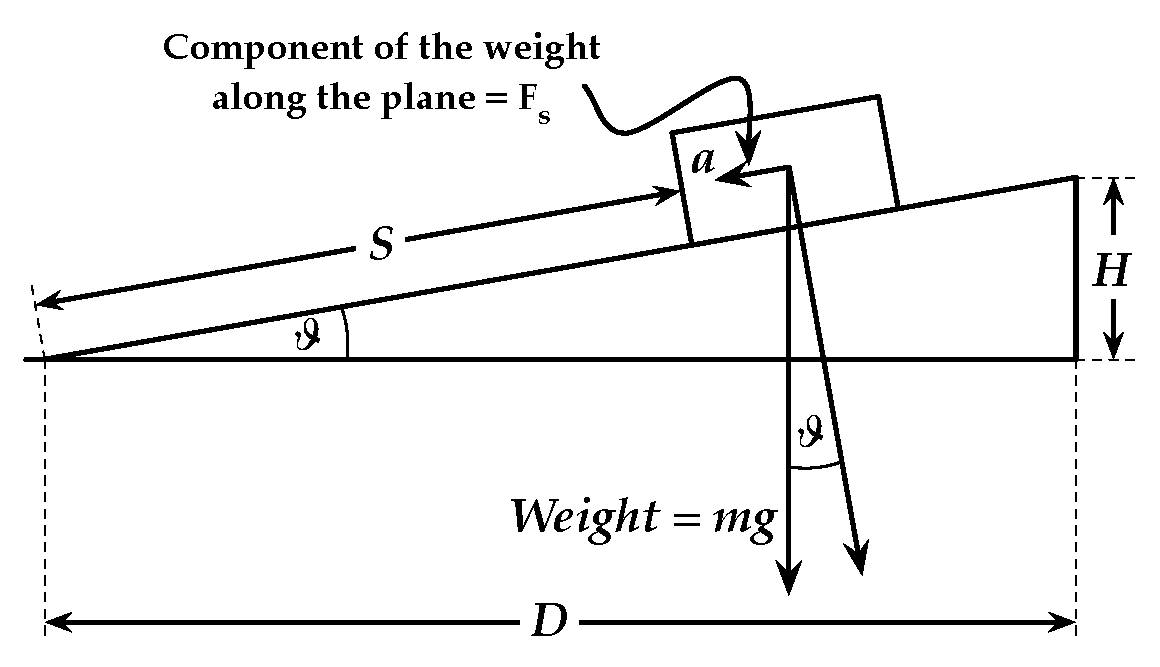
\includegraphics[width=5.5in]{Experiment02Figures/Figure01.pdf}
  \end{center}
  \caption{Force Diagram and variables used in Experiment M-\ref{lab:M2}.}
  \label{M02Fig01}  % the \label command comes AFTER the caption
\end{figure}

The displacement along the track is $S$ and the component of acceleration $a_s$ along the track is
\[
a_s = \frac{F_s}{m} = \frac{m g \sin(\theta)}{m} =  g \sin(\theta).
\]
If the mass is released from rest near the top of the inclined air track and allowed to accelerate down the air track with a magnitude $a_s$, then by measuring the transit time down the track over a measurable distance, $S$, we can determine the value of $g$.

Since the acceleration $a_s$ is constant, the displacement $S$ as a function of time $t$ is:
\[
  S = \frac{1}{2} a t^2 = \frac{1}{2} g t^{2} \sin(\theta).
\]
Solving for $g$, we obtain
\begin{equation}
  g = \frac{2 S}{t^2 \sin(\theta)}.
\end{equation}

If we assume that the incline angle $\theta$ is small, we can approximate the $\sin(\theta)$ by the $\tan(\theta) = \nicefrac{H}{D}$.
Making this substitution for the $\sin(\theta)$, we have the value of $g$ in terms of easily measurable quantities, namely
\begin{equation}
  \label{eq:M02gvalue}
  g = \frac{2 S D}{H t^2}
\end{equation}
where $H$ is the vertical rise in the horizontal distance $D$.  $D$ is the distance between the legs of the air track, and $t$ is the transit time of the mass, starting from zero velocity and accelerating down the plane a distance $S$ along the plane.
We will compare our results to the measured value of $g$ at sea level.  The value at sea level at New York is $g = 9.803\,\meter\per\second\squared$.

In the experiment, the presumed frictionless inclined plane will be an air track.  The mass will be a glider, which floats on the air track.  Placing a spacer of height $H$ under the leg at one end of the track, which is a distance $D$ from the leg(s) at the opposite end, will incline the track.  Refer to Fig.~\ref{M02Fig02} below in the experimental procedure section.

%\subsection{Acceleration by a hanging mass}
% --- removing, doesn't necessarily incorporate torque, doesn't add much to the lab at this point - 2024/08

%In this case you will use the \textbf{Capstone} program and the PASCO rotary sensor to measure $g$.
%Set the track level, with no spacer.
%The glider has mass $M_G$.
%A string connects the glider with a weight of mass $M_w = 10\,\gram$.
%The string passes over the large pulley of a PASCO rotary sensor.
%You have to account for the  mass of the rotating pulley to get a more accurate result.
%Your measured value for $g$ is found from
%\begin{equation}
%\label{eq:M2hanging}
%  M_w g = \left(M_G + M_{pulley} + M_w\right) a.
%\end{equation}
%Here $\left(M_G + M_{pulley} + M_w\right)$ is the total mass that is moving and $M_w g$ is the total force.
















\section{Experimental Procedure}

\begin{figure}[ht]
  \begin{center}
    %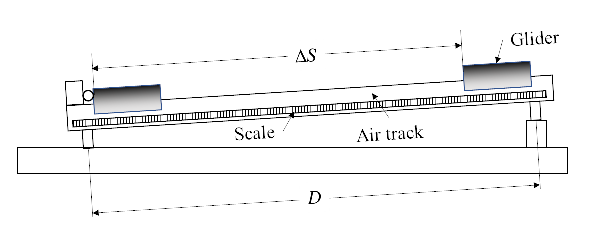
\includegraphics[width=5.6in]{Experiment02Figures/Figure02.eps}
    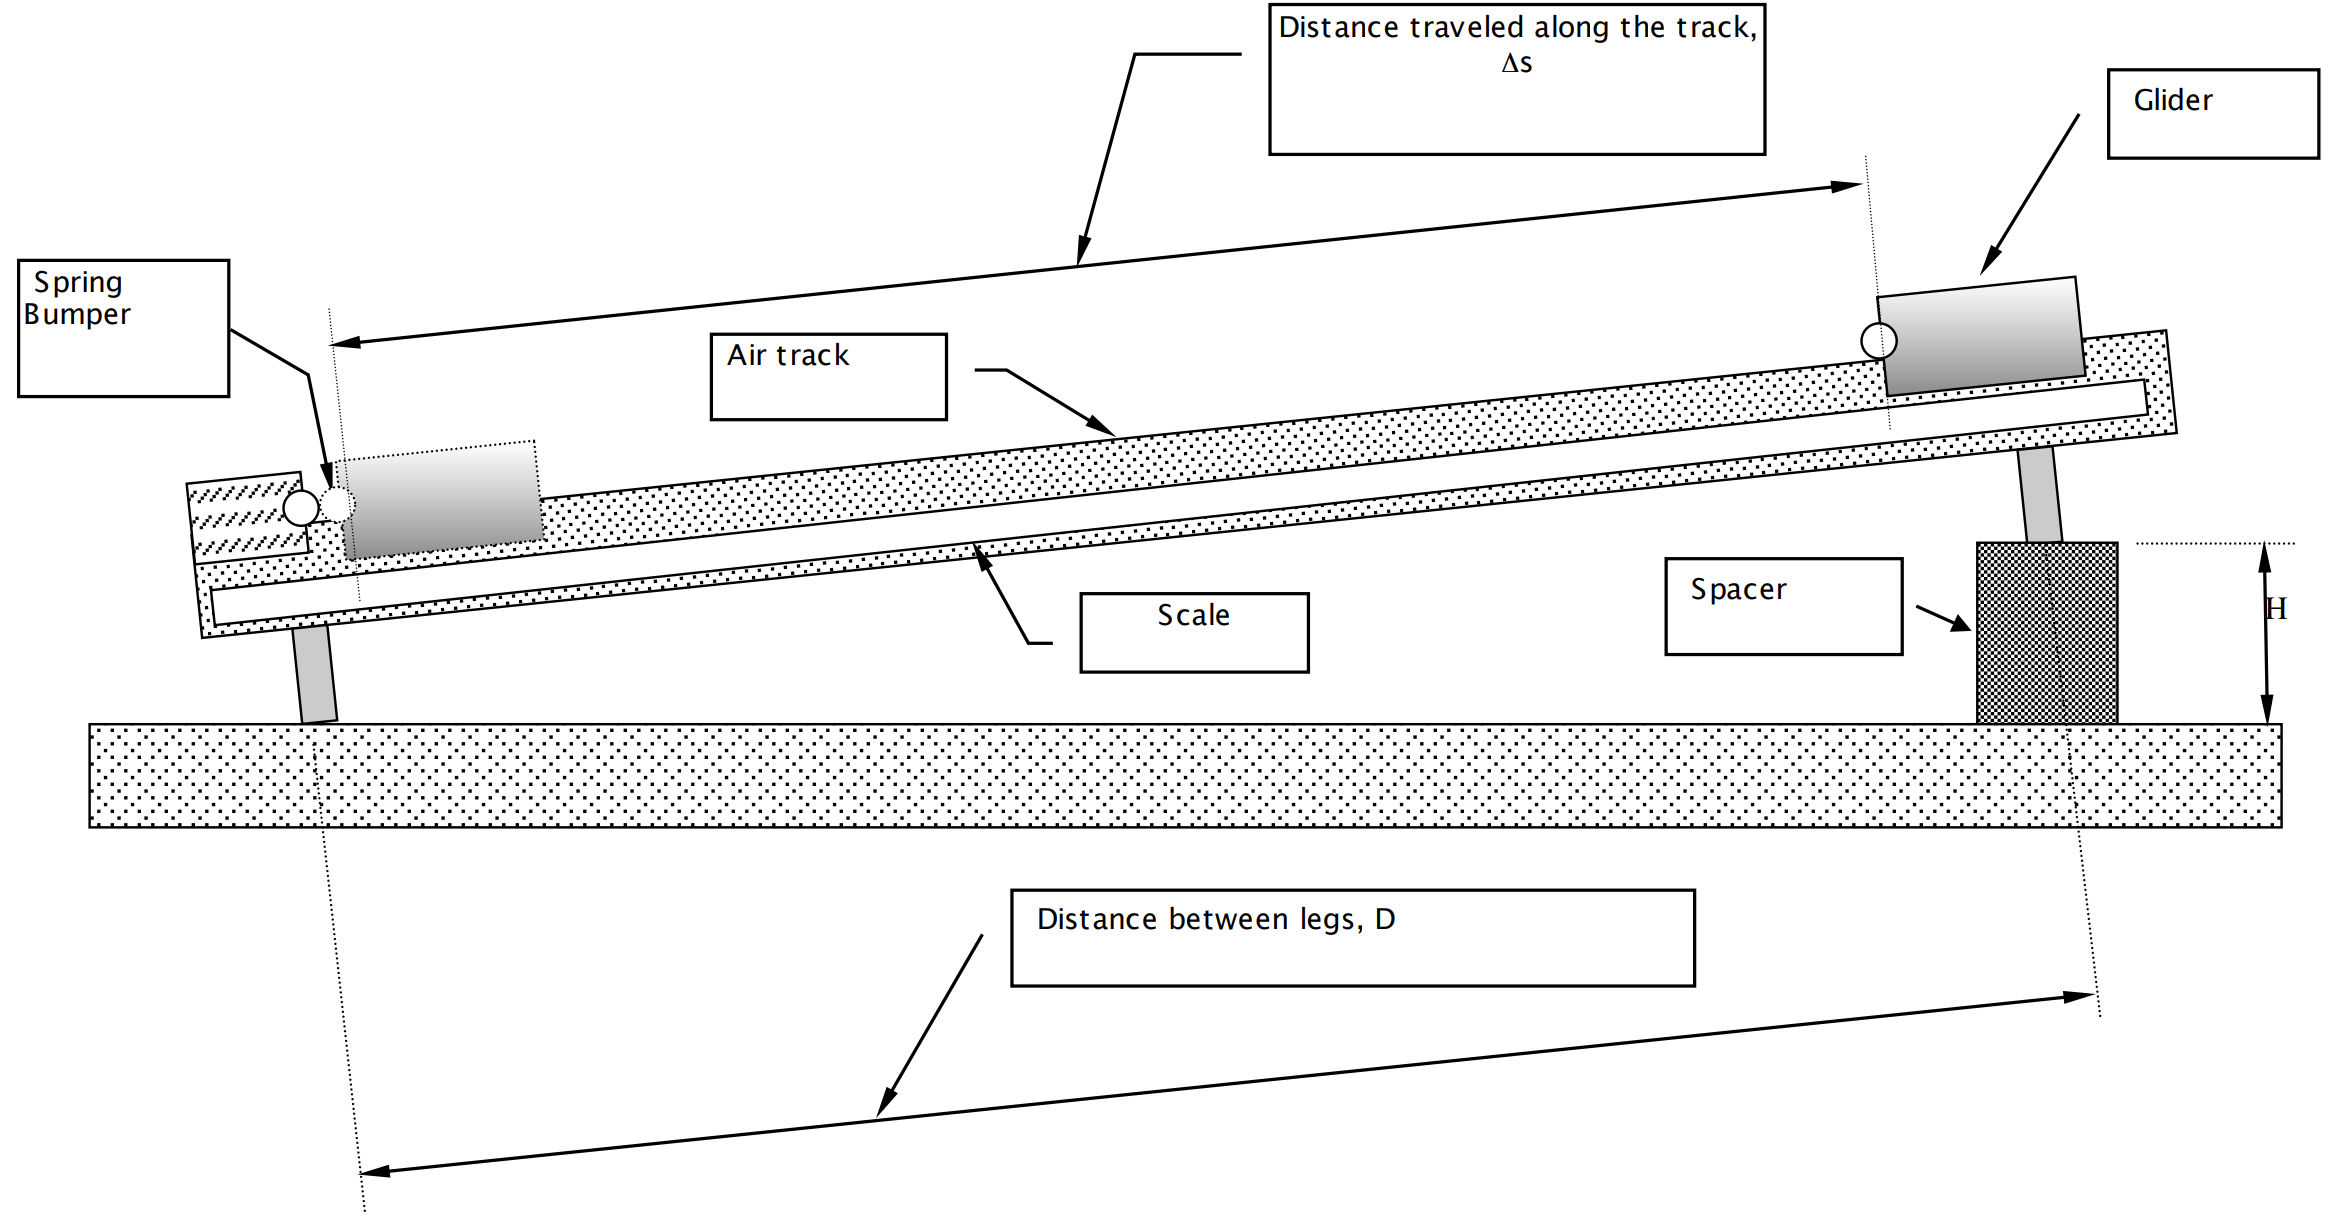
\includegraphics[width=5.8in]{Fall/Experiment02Figures/M02_fig2.png}
  \end{center}
  \caption{Experimental Setup for M-\ref{lab:M2}.}
  \label{M02Fig02}
\end{figure}

In this experiment you will measure the motion of a glider down a tilted track using PASCO photogates (stated precision of 0.0001 seconds) connected to PASCO's data logging and visualization software, \textbf{Capstone}, which will be set up as a timer for this experiment. 
\begin{enumerate}
\item %Turn on the air and allow it to run a couple of minutes before proceeding. It is very important that the track is clean and free of dirt. This will prevent any damage to the very expensive air track and will keep friction to an absolute minimum. 
\textbf{\textit{Do not put a glider on the track without air flowing.}}
\item Create a table of the common data including the masses of the gliders, the distance $D$ between the legs of the air track and the heights of the two spacers.
\item Measure and record the mass of both the large and small glider.
\item Without the spacer present and the air track resting directly on the tabletop (with the black circle feet), place one of the gliders on the track and note any preferential drift of the glider.  Adjust the height of the single leg (screw in or out) until the air track is level, as indicated by no preferential drift.  Check both orientations of the glider on the track to check if the car is asymmetric and has a significant preferential drift on an otherwise level track.  If this occurs, use another glider.
\item Measure and record the distance $D$.  This is the center-to-center distance between the legs.
\item Measure and record the heights, $H$, of each of the two spacers with the provided Vernier caliper for greater precision.
\item Four cases will be performed with a tilted air track, two gliders with two spacers (e.g. BIG spacer/small glider, BIG spacer/BIG glider, small spacer/small glider, small spacer/BIG glider).
%The final case will use a hanging mass to accelerate the glider.  
\item Determine a convenient point on the glider to use with the scale attached on the side of track.  It doesn't matter what point you choose, only that you use the same point for all determinations of $\Delta s$ for that glider.  A convenient point is the lower front or rear corner of the glider since it will be very close or overlapping with the length scale on the track itself.
%\item For each of the first four cases, perform the following steps and record the data appropriately in your spreadsheet:
\item For each of the four cases, perform the following steps and record the data appropriately in your spreadsheet:
  \begin{enumerate}
  \item For each of the four cases with a tilted track create enough \textbf{rows} for the number of trials you are doing, and \textbf{columns} for each of the variables you will be measuring or deriving:
    \begin{itemize}
      \item starting point at the top $s_1$
      \item stopping point at the bottom $s_0$
      \item distance between the photogates that the glider travels $S$
      \item start time at the top $t_1$
      \item time at the bottom $t_0$
      \item time between the photogates $\Delta t$
      \item calculated value of $g$ using Eqn.~\ref{eq:M02gvalue} for each of the five trials
      \item average value of $g$ from the five trials of each case
      \item standard deviation of $g$ from the five trials of each case
      \item difference between the average value of $g$ and the accepted value of $9.803\,\meter\per\second\squared$ for Fairfield, CT for each case
      \item similarly, the average, standard deviation, and difference for $g$ from all 20 trials across all 4 cases
      \end{itemize}
  \item Raise the single leg side of the track by placing a spacer under the knob.
  %\item Place the glider at the bottom of the track resting against the bumper. Record $s_{0}$. (Note: With the car at this position, the red light on the bottom photogate should be lit. Moving the glider to the right the slightest distance should put the light out. If this is not the case, adjust the position of the photogate.)
  \item Place the glider near the bottom of the track. Move it slowly as you approach the bottom photogate. Stop the glider at the exact location when the photogate's red light comes on. Record position on the scale, $s_0$.
  \item Next, place the glider near the top of the track. Move it slowly as you approach the top photogate. Stop the glider at the exact location when the photogate's red light comes on. Record position on the scale, $s_1$.
  %\item Before you take the recorded data in the next step, take some practice runs. Your subsequent data will be much improved by your training! Set the photogate timer to pulse mode. Position the glider so it is blocking the top photogate and the red light is on. Place one finger on the track in front of the glider and gently push the glider to the right until the red light on the photogate just goes out. Press the reset button on the timer. Release the glider by quickly pulling your finger away from the track. After the glider bounces off the lower bumper, the time of travel from top to bottom will be displayed on the timer.
  \item Before you take the recorded data in the next step, take some practice runs. Your subsequent data will be much improved by your training! Press record in \textbf{Capstone} to start the timer. \textit{NOTE: }\textbf{Capstone} will display the time whenever a photogate beam is broken; the time at the higher (start) photogate $t_1$ as well as the time at the lower (end) photogate $t_0$. To determine the total transit time $\Delta t$, take the difference of the start and end times.
  \item Position the glider so it is blocking the top photogate and the red light is on. Place one finger on the track in front of the glider and gently move the glider up the track (to the right) until the red light on the photogate just goes out.
  \item Release the glider by quickly pulling your finger away from the track and glider (MINIMIZE ANY FINGER CONTACT WITH THE GLIDER to minimize any additional push or pull on the glider to \textbf{ensure its initial velocity is zero}). 
    \item For each of the \textbf{5 trials per case}, release the glider from rest at the $s_1$ position. Measure and record the start time $t_1$ and end time $t_1$ to determine transit time $\Delta t$ from release at the top to bottom of the airtrack. Calculate the value of $g$ for this trial.
















    
  \end{enumerate}





  \item For each the four cases:
\begin{itemize}

  \item Calculate the average of the measured $g$
  \item Calculate the standard deviation of the measured $g$
  \item Calculate the differences between your average $g$ and the accepted value of $g$
  %\item Create a new table for the acceleration of the glider with the hanging mass.  including:
  %  \begin{itemize}
  %    \item the glider $M_G$, the pulley $M_{pulley}$, and the hanging weight $M_w$ masses,
  %    \item the acceleration $a_G$ of the glider,
  %    \item the experimental value of $g$ using Eqn.~\ref{eq:M2hanging}.
  %  \end{itemize}
\end{itemize} 

  \item Also, using data from all trials from all the cases:
  \begin{itemize}
    \item Calculate the average of the measured $g$.
    \item Calculate the standard deviation of the measured $g$.
    \item Calculate the differences between your average $g$ and the accepted value of $g$
  \end{itemize}

\end{enumerate}

%The next experiment is performed by accelerating the glider along a level track with a hanging weight.  You will use the Capstone program and the PASCO rotary sensor. 
%\begin{itemize}
%\item Remove the spacers and return the track to level. 
%\item Turn on the air and allow it to run a couple of minutes before proceeding. It is very important that the track is clean and free of dirt. This will prevent any damage to the very expensive air track and will keep friction to an absolute minimum. Do not put a glider on the track without air flowing.
%\item Attach the string provided to red glider with mass $M_G$.
%Pass the string over the large pulley of the rotary sensor.
%Hang a $M_w = 10$ gram weight on the string.
%\item Pull the glider along the track until the hanging weight is near the pulley and hanging freely.
%\item Start recording using the \textbf{Capstone} program. See page~\ref{sec:SettingUpHardware}.
%\item Release the glider. The mass will fall, rotate the pulley and pull the glider.
%\item Stop recording once the glider hits the end of the track.
%\item Record the slope of the line which is the acceleration $a_G$ of the glider. Calculate $g$ using Eqn.~\ref{eq:M2hanging} with $M_{pulley} = 6\,\gram$.
%\end{itemize}












%\section{Data Analysis}













\section{Post-Lab Submission --- Interpretation of Results}

\begin{itemize}

\item Make sure to submit your finalized data table (Excel sheet)

\item If you release the glider higher above the photogate rather than right at the gate, what would you expect to happen to your derived values of $g$? 
\item What are sources of uncertainty (initial v, friction, etc.)?
\item What was the precision of the instrumentation (e.g. caliper, time, distance, etc.)?
\item Compare your results ($g$ from each of the four cases and one from all 20 trials) to the accepted value. How do the standard deviations compare to the difference between your values of $g$ and the accepted value of $g$? I.e. while treating the standard deviations of your measurements as your measurement uncertainties, do your values of $g$ for each case, as well as the overall average $g$, plus or minus the standard deviations overlap (and agree) with the accepted value of $g$? What might cause your results to disagree the most?
\item Suppose there is a frictional force slowing the glider as it moves along the track. How would this affect the determined value of $g$? Would your result support or not support the hypothesis of that there is significant friction along the track?
\item Assume the track is not level at the beginning of the experiment. Further, assume that what you thought to be a level track was in fact slightly tipped in the same direction as your deliberate tipping via the spacers during the experiment. How would this affect the determined value of $g$? Would your result support or not support the hypothesis of the track not being level?



%\item Calculate the average value of $g$ from all your measurements and determine the difference between your result and the commonly accepted value of $9.803\,\meter\per\second\squared$.
%\item Suppose there is a frictional force slowing the glider as it moves along the track. Explain the effect on the measurement of the value of $g$ and state whether your result would support the hypothesis of friction along the track.
\end{itemize}


\newpage
\text{ }
%%%%%%%%%%%%%%%%%%%%%
%                                             %
%                 Experiment M-3              %
%               g with a pendulum             %
%                                             %
%%%%%%%%%%%%%%%%%%%%%

% Hyperref doesn't like math in chapter titles.
\iffalse
\labChapter{M}{Simple Projectile Motion with Kinematics}
\else
\labChapter{M}{Simple Projectile Motion with Kinematics}
\fi
\label{lab:M3}






% Background
\section{Background}


\textbf{Projectile motion} is the motion of an object thrown or projected into the air, subject only to acceleration as a result of gravity. The applications of projectile motion in physics and engineering are numerous. Some examples include meteors as they enter Earth’s atmosphere, water in a water fountain, and the motion of any ball in sports. Such objects are called \textit{projectiles}, and their path is called a \textbf{trajectory}. 

We can represent a projectile's motion through kinematics which utilize its position, time, velocity, and acceleration. The kinematic equations we will use during this lab assume both \textbf{\textit{constant acceleration}} effects of air resistance are \textbf{\textit{negligible}} (generalized in the next four equations with $x$ representing position along any given dimension):

 \begin{equation}
  \label{eq:M03Kinematic_01}
  v = v_{0} + at
\end{equation}


 \begin{equation}
  \label{eq:M03Kinematic_02}
  x = x_{0} + v_{0}t + \frac{1}{2}at^{2}
\end{equation}


 \begin{equation}
  \label{eq:M03Kinematic_03}
  v^{2} = v_{0}^{2} + 2a(x - x_{0})
\end{equation}

 \begin{equation}
  \label{eq:M03Kinematic_04}
  x = x_{0} + \frac{1}{2}(v_{0} + v)t
\end{equation}



\pagebreak


Today, we will analyze both one- and two-dimensional trajectories, where $x$ will represent the horizontal direction, and $y$ the vertical. Gravity (which pulls objects down towards the center of the Earth) will be assumed to be the only source of acceleration acting on our projectiles; as such, the acceleration of a projectile is $a_{y} = -g$ and $a_{x} = 0$. Since horizontal acceleration terms are zero, we can represent horizontal motion by:

 \begin{equation}
  \label{eq:M03horizontalKinematic}
  v_{0x} = v_{x} = \text{constant velocity},~~~ x = x_{0} + v_{x}t
\end{equation}

Then, depending on the information we have available to us, we can represent vertical motion by:

 \begin{equation}
  \label{eq:M03Kinematic_vertical_01}
  v_{y} = v_{0y} - gt
\end{equation}


 \begin{equation}
  \label{eq:M03Kinematic_vertical_02}
  y = y_{0} + v_{0y}t - \frac{1}{2}gt^{2}
\end{equation}


 \begin{equation}
  \label{eq:M03Kinematic_vertical_03}
  v_{y}^{2} = v_{0y}^{2} - 2g(y - y_{0})
\end{equation}

 \begin{equation}
  \label{eq:M03Kinematic_vertical_04}
  y = y_{0} + \frac{1}{2}(v_{0y} + v_{y})t
\end{equation}







\underline{\textbf{Free Fall / Downward Trajectory (First experiment)}}

In the previous lab, we determined the acceleration due to gravity via the tilted air track to take advantage of a longer time frame to measure a small fraction of the acceleration due to gravity. This week, we will determine the acceleration due to gravity more directly by considering a one-dimensional trajectory (i.e. free fall).



The experimental setup will involve a free-fall timer where a metal ball is dropped from a release mechanism as shown in Fig.~\ref{M03_simpleProjectileLauncher_Exp1}. When the metal ball is in then mechanism, it provides a closed circuit; once the ball is released and the circuit opens, the computer automatically starts timing $t_{\text{initial}}$. The ball then hits the receptor pad on the floor, closing the circuit and stopping the timer at $t_{\text{final}}$. Using the recorded time difference $t = t_{\text{final}} - t_{\text{initial}}$, and the initial height $y_{0}$ as measured from the bottom of the ball to the top of the receptor plate (which is at the final height $y = 0\,\meter$), we can rearrange Eqn.~\ref{eq:M03Kinematic_vertical_02} to determine acceleration due to gravity.

 \begin{equation}
  \label{eq:M03Kinematic_freefall_g}
  0 = y_{0} + 0 - \frac{1}{2}gt^{2}~~~=>~~~\frac{2y_{0}}{t^2} = g
\end{equation}

\begin{figure}[h]
  \begin{center}
    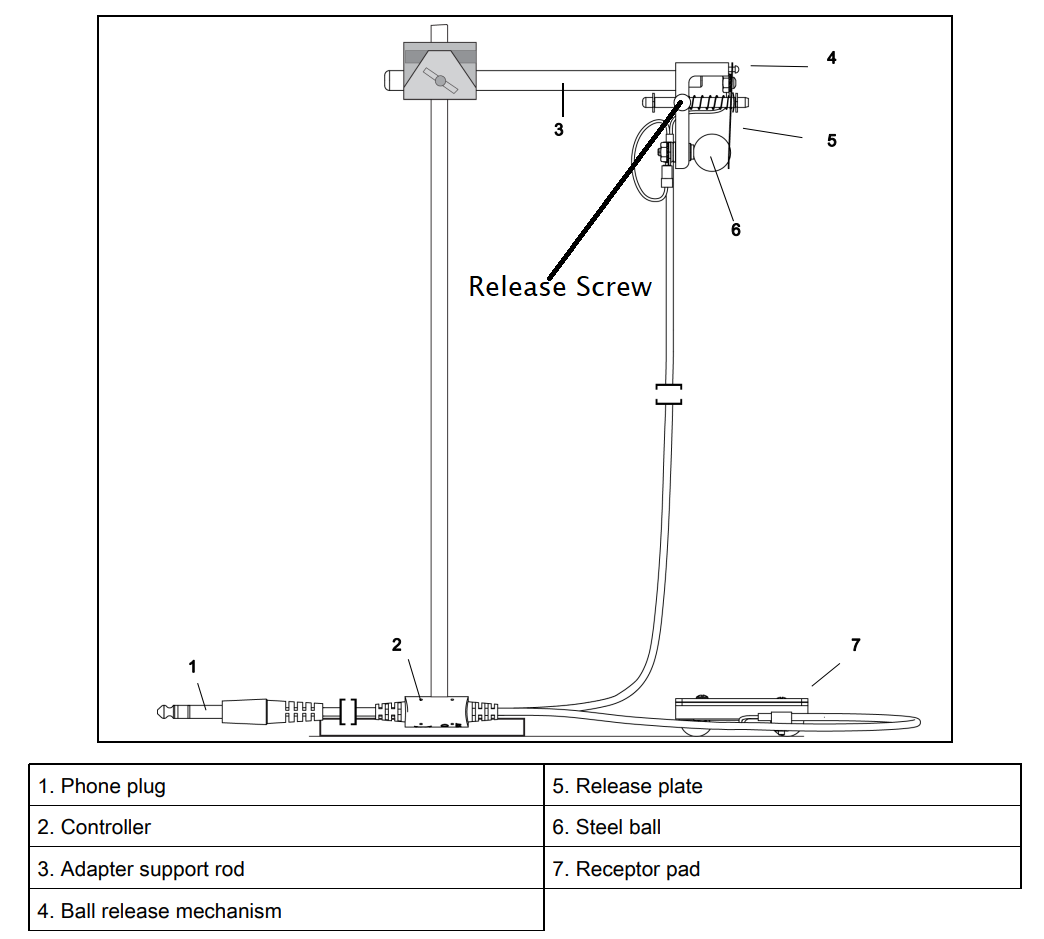
\includegraphics[width=4.9in]{Fall/Experiment03FiguresNEW/M3_Exp1.png}
  \end{center}
  \caption{Example of the free fall apparatus used in Exp. 1. Note the release screw will be what you tighten or loosen to hold or release the ball from the release mechanism.}
  \label{M03_simpleProjectileLauncher_Exp1}
\end{figure}

\pagebreak

\underline{\textbf{Horizontal Trajectory (Second experiment)}}


\begin{figure}[h]
  \begin{center}
    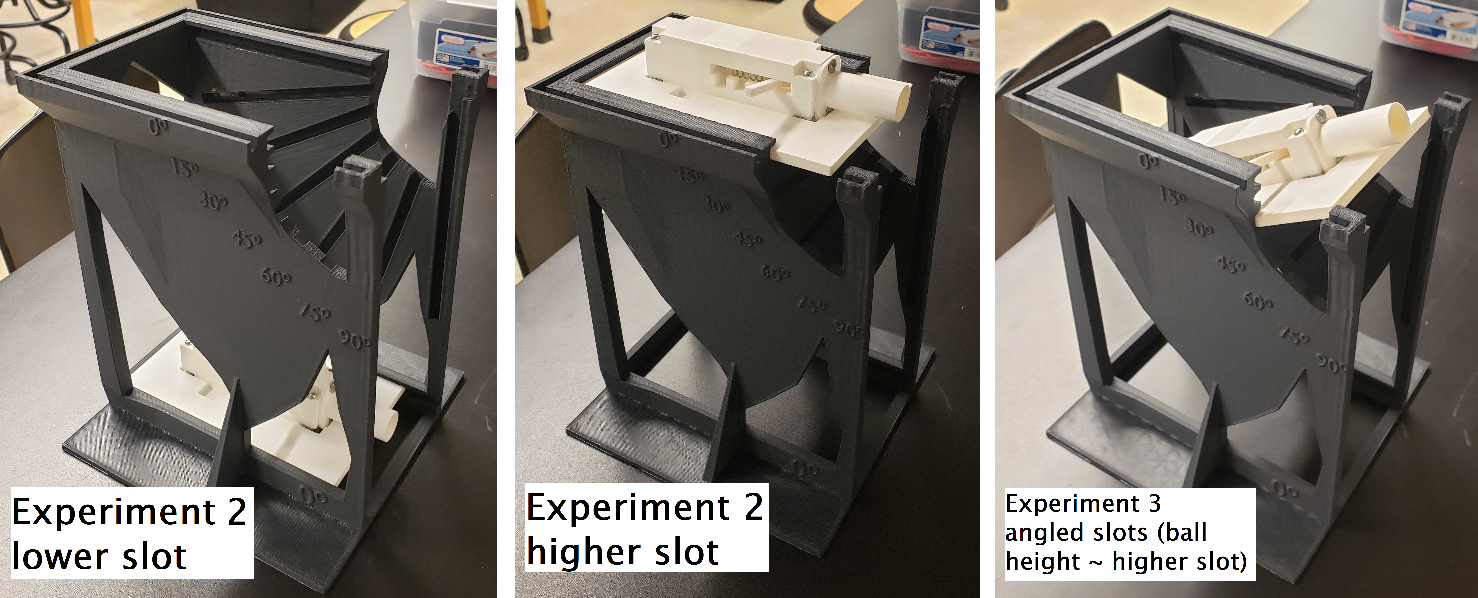
\includegraphics[width=5.9in]{Fall/Experiment03FiguresNEW/M3_ExpOptions_quarter_size.png}
  \end{center}
  \caption{Left) Position of launcher for lower height in Experiment 2. Right) Position of launcher for higher height in Experiment 2. Right) Position of launcher for angled launches in Experiment 3 where the ball's initial position is the same as the higher height position.}
  \label{M03_simpleProjectileLauncher}
\end{figure}


Note: For this experiment as well as the third experiment later on, while we could use our determined value for gravity, for simplicity, we will instead use the accepted value of $g = 9.803\,\meter\per\second\squared$ for Fairfield, CT.

In this second experiment, we will \textbf{1)} first investigate the horizontally launched trajectory of the same metal ball used in the first experiment (launched at 90$\degree$ relative to $g$, or 0$\degree$ relative to the floor). Then \textbf{2)} we will attempt to estimate where the ball will land when launched from a different height and see how accurate we are.

This setup will involve a marble launcher that can slide into a large holder at different initial heights $y_{0}$ (and later for the third experiment, different angles, see Fig.~\ref{M03_simpleProjectileLauncher}). Height $y_{0}$ will be measured from the bottom of the ball (effectively the bottom inside of the launcher's barrel) to the floor. Once the ball is released, it will begin a two-dimensional trajectory accelerated solely by gravity in the $y$ direction.

\underline{\textbf{-1-)}} The distance in the $x$ direction will be measured from the center of the ball in the uncocked position (a plum bob can be used to find the ball's initial position on the floor) to the average landing position on the floor after the given number of trials. The ball will mark up paper with carbon paper; we will circle this scatter shot and estimate the average position of all trials from the given case, and then measure the distance with a 1 or 2 meter stick to determine $x$.

After investigating how far the ball travels in the $x$ direction from a given height, we can determine characteristics about the launcher-and-ball system to estimate how far in the $x$ direction we may expect the ball to travel in the second part of this experiment when we launch it from a different initial height. To estimate how far the ball will travel, we can use Eqn.~\ref{eq:M03horizontalKinematic} to determine $x$. However, to do so, we will need to for how long and how fast it was moving (distance traveled = speed $\times$ time). Since we know the initial height $y_{0}$ of the ball, we can determine the time $t$ it took to fall to the floor in the $y$ direction due solely to gravity $g$ by rearranging Eqn.~\ref{eq:M03Kinematic_vertical_02} to solve for $t$, knowing that $v_{0y} = 0\,\meter\per\second$ and treating the floor as $y = 0\,\meter$:

 \begin{equation}
  \label{eq:M03Kinematic_vertical_time}
  0 = y_{0} + 0 - \frac{1}{2}gt^{2}~~~=>~~~\sqrt{\frac{2y_{0}}{g}} = t
\end{equation}

Now that we know the time $t$ of the trajectory, and treating the uncocked position as $x_{0} = 0\,\meter$, we can use Eqn.~\ref{eq:M03horizontalKinematic} to determine the horizontal velocity $v_{x}$ when released:

 \begin{equation}
  \label{eq:M03Kinematic_horizontal_velocity_01}
  x = 0 + v_{x}t~~~=>~~~\frac{x}{t} = v_{x}
\end{equation}

\underline{\textbf{-2-)}} For the second part of this experiment, we move the launcher to the higher $0\degree$ slot ($\sim20\,\centi\meter$ higher), and we want to determine how far it will travel in the $x$ direction. This leads us back to Eqn.~\ref{eq:M03horizontalKinematic} where we want to solve for $x_{\text{higher height}}$ (where again, $x_{0} = 0\,\meter$ in the uncocked position):

 \begin{equation}
  \label{eq:M03Kinematic_horizontal_velocity_02}
  x = 0 + v_{x}t~~~=>~~~x_{\text{higher height}} = v_{x}t_{\text{higher height}}
\end{equation}

We know the ball's velocity $v_{x}$, but we no longer know the time. However, similar to before, we can solve for $t_{\text{higher height}}$ by plugging $y_{0\text{,higher height}}$ into Eqn.~\ref{eq:M03Kinematic_vertical_time}:

 \begin{equation}
  \label{eq:M03Kinematic_vertical_time_higher_height}
  \sqrt{\frac{2y_{0\text{,higher height}}}{g}} = t_{\text{higher height}}
\end{equation}

This subsequent value for time $t_{\text{higher height}}$ can be used in Eqn.~\ref{eq:M03Kinematic_horizontal_velocity_02} to then calculate a theoretical distance $x_{\text{higher height, theoretical}}$. We will then launch the ball from this higher height see how accurate we estimated $x_{\text{higher height, theoretical}}$. The experimentally determined $x_{\text{higher height, experimental}}$ will be measured in the same way as the first part of this experiment (circling and estimating the center of the scattershot).



\underline{\textbf{Angled Trajectory (Third experiment)}}




The third part of this experiment is similar to the 2nd part of the second experiment in that we are staying at the higher height, but now investigating the trajectories when launched from different angles, namely, how far in the $x$ direction do they reach? The large, launcher holder is designed to hold the ball at rest (uncocked) in the same position (height) regardless of angle, so you should be able to use your previously determined $y_{0\text{,higher height}}$ as your value for the ball's initial height (see Fig.~\ref{M03_simpleProjectileLauncher} right).

By launching at an upward angle $\theta$, we are now giving some of the initial velocity to both $x$ and $y$ directions. Once again, as there is no acceleration in the $x$ direction, we will ultimately use Eqn.~\ref{eq:M03horizontalKinematic} to determine $x_{\theta}$. However, we need to know both $v_{x\theta}$ and $t_{\theta}$. The velocity will merely be the horizontal component of the launch angle:


 \begin{equation}
  \label{eq:M03Kinematic_horizontal_velocity_03}
    v_{x\theta} = v_{x}\cos{\theta} 
\end{equation}

\begin{figure}[h]
  \begin{center}
    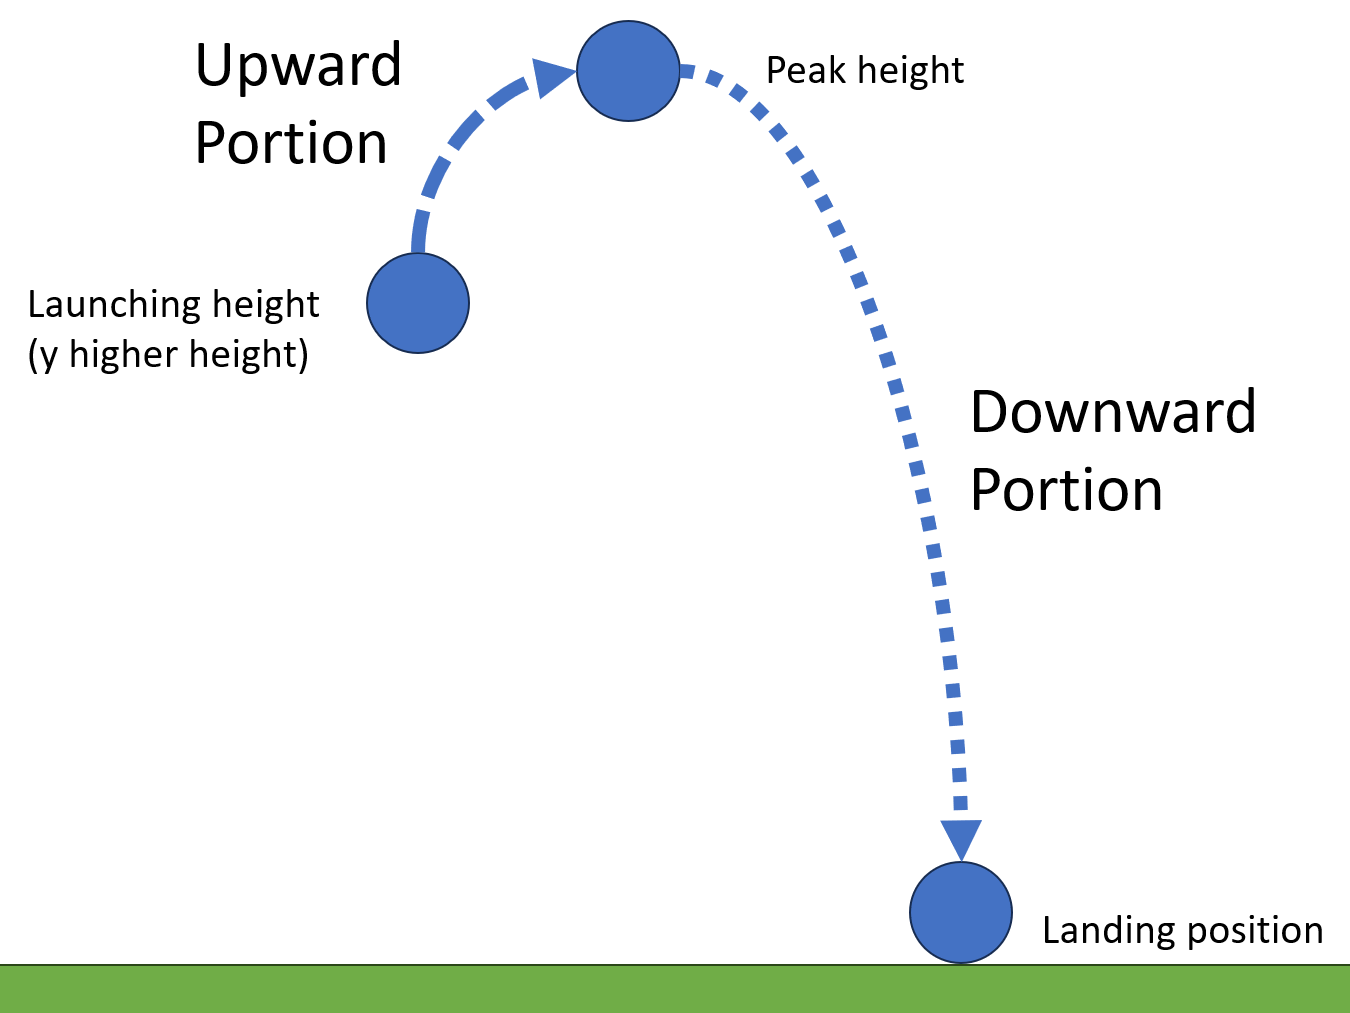
\includegraphics[width=3.9in]{Fall/Experiment03FiguresNEW/M3_Exp3.png}
  \end{center}
  \caption{Example of the upward and downward portions you'll analyze in Experiment 3 for an angled launch.}
  \label{M03_simpleProjectileLauncher_Exp3}
\end{figure}

To solve for the time, however, we can characterize motion in the $y$ direction to determine for how long the ball is in the air.
%Using the same process as before where the floor is at $y_{0} = 0\,\meter$, and $v_{0y} = v_{x}\sin{\theta}$, we can find $t_{\theta}$ 
%using Eqn.~\ref{eq:M03Kinematic_vertical_02} and the quadratic formula:
%
%
% \begin{equation}
%  \label{eq:M03Kinematic_vertical_time_03}
%  y = 0 + v_{0y}t - \frac{1}{2}gt^{2}~~~=>~~~y = 0 + v_{x}\sin{\theta}t_{\theta} - \frac{1}{2}gt_{\theta}^{2}~~~=>
%\end{equation}
%
%
% \begin{equation}
%  \label{eq:M03Kinematic_vertical_time_03_pt2}
% =>~~~\frac{1}{2}gt_{\theta}^{2} - v_{x}\sin{\theta}t_{\theta} + y = 0~~~=>~~~t_{\theta} = \frac{-(-v_{x}\sin{\theta}) \pm \sqrt{((-v_{x}\sin{\theta})^2 - 4\frac{g}{2}y)}}{2\frac{g}{2}}
%\end{equation}
%
% \begin{equation}
%  \label{eq:M03Kinematic_vertical_time_03_pt3}
% =>~~~t_{\theta} = \frac{v_{x}\sin{\theta} \pm \sqrt{((-v_{x}\sin{\theta})^2 - 2gy)}}{g}
%\end{equation}
%
%Note: we would take the larger value as we are launching the ball upwards rather than the smaller value that would represent shooting down towards the floor.
%
As shown in Fig.~\ref{M03_simpleProjectileLauncher_Exp3}, we can find that total time by breaking the trajectory into parts (i.e. $t_{\theta}~=~t_{\text{up}}~+~t_{\text{down}}$) where $t_{\text{up}}$ is the time for upward travel to the peak height, and $t_{\text{down}}$ is the time for downward travel to the floor from that peak height. \textbf{UPWARD PORTION)} Starting with Eqn.~\ref{eq:M03Kinematic_vertical_01}, where we know for the upward travel portion the initial velocity in the $y$ direction is $v_{0y} = v_{0y\text{ higher height}} = v_{x}\sin{\theta}$ and at the peak of the trajectory (end of the upward travel) $v_{y} = v_{y\text{peak}} = 0\,\meter\per\second$, thus:

 \begin{equation}
  \label{eq:M03Kinematic_vertical_time_03_v2_pt1}
  v_{y\text{ peak}} = v_{0y\text{ higher height}} - gt~~~=>~~~0 = v_{x}\sin{\theta} - gt_{\text{up}}~~~=>~~~\frac{v_{x}\sin{\theta}}{g} = t_{\text{up}}
\end{equation}

\textbf{DOWNWARD PORTION)} Then for the downward travel, we need to first know how high we travelled during the upward portion (i.e. $y_{0\text{,higher height}} \text{ to } y_{\text{ peak}}$) so we can use Eqn.~\ref{eq:M03Kinematic_vertical_02} later to determine the time it took to fall from $y_{\text{ peak}} \text{ to } y_{\text{ floor}}$. Since we know our initial height $y_{0} = y_{0\text{,higher height}}$, initial velocity $v_{0} = v_{0y\text{ higher height}} = v_{x}\sin{\theta}$, and the time it took to get $t_{\text{up}}$ there from Eqn.~\ref{eq:M03Kinematic_vertical_time_03_v2_pt1}, we can use Eqn.~\ref{eq:M03Kinematic_vertical_02} to solve for the final height of the upward travel $y_{\text{peak}}$:

 \begin{equation}
  \label{eq:M03Kinematic_vertical_time_03_v2_pt2}
  y_{\text{peak}} = y_{0\text{,higher height}} + v_{x}\sin{\theta}t_{\text{up}} - \frac{1}{2}gt_{\text{up}}^{2}
\end{equation}


Now that we know $y_{\text{peak}}$, we can use Eqn.~\ref{eq:M03Kinematic_vertical_02} to solve for $t_{down}$, this time with the final height $y_{\text{floor}} = 0\,\meter$, initial height of $y_{\text{peak}}$, and the initial velocity $v_{y\text{ peak}} = 0\,\meter\per\second$.


 \begin{equation}
  \label{eq:M03Kinematic_vertical_time_03_v2_pt3}
  y_{\text{floor}} = y_{\text{peak}} + v_{y\text{ peak}} - \frac{1}{2}gt_{\text{down}}^{2}~~~=>~~~0 = y_{\text{peak}} + 0 - \frac{1}{2}gt_{\text{down}}^{2}~~~=>~~~\sqrt{\frac{2y_{\text{peak}}}{g}} = t_{\text{down}}
\end{equation}


\textbf{HORIZONTAL DISTANCE)} Finally, we have the total time $t_{\theta}~=~t_{\text{up}}~+~t_{\text{down}}$ from Eqns.~\ref{eq:M03Kinematic_vertical_time_03_v2_pt1} and ~\ref{eq:M03Kinematic_vertical_time_03_v2_pt3} and the initial velocity $v_{x}$ from Eqn.~\ref{eq:M03Kinematic_horizontal_velocity_03} to incorporate into Eqn.~\ref{eq:M03horizontalKinematic} to determine the theoretical distance $x_{\theta}$ the ball with travel in the $x$ direction for any given angle $\theta$:

 \begin{equation}
  \label{eq:M03Kinematic_vertical_time_03_v2_pt4}
  x_{\theta} = v_{x}\cos{\theta}t_{\theta}
\end{equation}



%Experimental Procedure
\section{Experimental Procedure}


\subsection{EXPERIMENT 1 -- Free Fall / Downward Trajectory}


%\TEXTBF{FIRST EXPERIMENT} We study one-dimensional trajectory (free fall)


\begin{enumerate}
\item \textbf{OVERALL GOALS:} 
\begin{itemize}
    \item Investigate projectile motion in one-dimension ($y$).
    \item Conduct 5 trials of the free-fall and determine acceleration due to gravity using one-dimensional kinematics.
    \item \textit{POINT TO CONSIDER}: Will this experiment be more or less accurate in measuring $g$ than the previous lab using gliders on a tilted air track?
    \item \textit{NOTE}: There are only 4 setups, please share, and once you're done taking your data, move on to ensure other groups have a reasonable chance to use the apparatus.
    %\textit{TO CONSIDER}: On the moon, would the ball fall faster, slower, or the same speed as ?
    \item PASCO TIMER Precision: 0.0001 seconds
\end{itemize}


\item Create a data table for this experiment:
\begin{itemize}
    \item Common data section with the accepted value of $g$, the ball height $y_{0}$, and the ball height's estimated uncertainty $\delta y$.
    \item With \textbf{five rows} (1 for each of the 5 free-fall trials). Also include additional \textbf{rows} for the average $g$ value, the $\pm$ uncertainty in gravity $\delta g$, the magnitude difference compared to the accepted $g$ \textit{DISCUSSION POINT for later}: How well does you average value of $g \pm \delta g$ agree with the accepted value of $g$?).
    \item Include \textbf{six columns} for
    \begin{itemize}
        \item Initial time $t_{\text{initial}}$
        \item Initial time uncertainty $\delta t_{\text{initial}}$
        \item Final time $t_{\text{final}}$
        \item Final time uncertainty $\delta t_{\text{final}}$
        \item Total elapsed time $t = t_{\text{final}} - t_{\text{initial}}$
        \item Total elapsed time uncertainty $\delta t = t_{\text{final}} - t_{\text{initial}}$
        \item Calculated $g$
    \end{itemize} 
\end{itemize}
\item CAPSTONE will be set up with the Free-Fall Adapter which, whenever the circuit opens or closes, will record the time that event occurred.
\item Place your metal ball from your marble launcher into the spring loaded holder at one of the four setups. You will need to push the metal tab in and then hand-tighten the holding/release screw to hold the ball in place.
\item Ensure the receptor pad is beneath the ball such that it hits close to the open side.
\item Measure the height the ball will fall; the initial height $y_{0}$ is measured from the bottom of the ball to the top of the receptor plate which has a final height $y = 0\,\meter$ if you place the meter stick on the receptor pad.
\item Press Record in CAPSTONE. You can let it run and it'll continue collecting data even when you reset the ball for additional trials; or restart for each trial, just be aware of which data points are related to your drop.
\item Unscrew the holding/release screw to allow the ball to fall.
\item Record your $t_{\text{initial}}$ and $t_{\text{final}}$ times.
\item Repeat the drop for a total of 5 free-fall trials. Determine the total elapsed times $t$ for each trial.
\item Using Eqn.~\ref{eq:M03Kinematic_freefall_g}, calculate the value of $g$ for each of your trials (benefit here of calculating $g$ from each trial: you can more easily notice any outlier data).
\item Determine your average $g$ from the preceding values.
\item Estimate your uncertainty in $g$, as represented by $\delta g = g_\text{test} - g$, (i.e. how confident [$\pm$] you are in what you measured -- e.g. distance, time). Plug in each measurements' uncertainties to make your test value of $g_\text{test}$ as calculated with Eqn.~\ref{eq:M03Kinematic_freefall_g} as big as possible (i.e. larger numerator, smaller denominator). Determine $\delta g$.
\item Compare your average $g$ to the accepted value of $g = 9.803\,\meter\per\second\squared$; what is the total difference?
%\item Compare your average $g$ to the accepted value of $g = 9.803\,\meter\per\second\squared$; what is the \% difference?
\item Does you average $g \pm \delta g$ cover the difference from the accepted value and agree, or not?

\end{enumerate}


\subsection{Horizontal Trajectory (Second experiment)}



\begin{enumerate}
\item \textbf{OVERALL GOALS:} 
\begin{itemize}
    \item Investigate projectile motion in two-dimensions when launched horizontally.
    \item For simplicity and to decrease error propagation, \textbf{for the rest of lab, assume and use} the accepted value of $g = 9.803\,\meter\per\second\squared$ for Fairfield, CT rather than your previously determined value.
    \item Characterize the trajectory from the marble launcher at initial height.
    \item Calculate the theoretical trajectory (distance $x$) for a different height; place a bullseye at your expected location and compare your experimental landing scattershot to the theoretical distance.
    \item Conduct 20 launches for each height; estimate the experimental landing scattershot by circling your carbon-paper dots and estimating the center of the scattershot.
    %\item \textit{POINT TO CONSIDER}: Will this experiment be more or less accurate in measuring $g$ than the previous lab using gliders on a tilted air track?
    %\item \textit{NOTE}: There are only 4 setups, please share, and once you're done taking your data, move on to ensure other groups have a reasonable chance to use the apparatus.
    %\textit{TO CONSIDER}: On the moon, would the ball fall faster, slower, or the same speed as ?
\end{itemize}


\item Create a data table for this experiment:
\begin{itemize}
    \item Common data section with the accepted value of $g$.
    \item Section for the case at a the lower initial height containing:
    \begin{itemize}
        \item the ball height $y_{0}$
        \item the ball height's estimated uncertainty $\delta y_{0}$
        \item distance $x$
        \item distance uncertainty $\delta x$ based on the radius of the circle you draw around the scattershot
    \end{itemize} 
    \item Additional sections for derived time of the trajectory $t$ and velocity $v_{x}$
    \item Additional sections for:
    \begin{itemize}
        \item Height of the ball at the higher $0 \degree$ slot height $y_{0\text{,higher height}}$
        \item Time of the trajectory from a higher height $t_{\text{higher height}}$
        \item Theoretical distance $x_{\text{higher height, theoretical}}$ (calculated with Eqn.~\ref{eq:M03Kinematic_horizontal_velocity_02})
        \item Experimentally measured distance $x_{\text{higher height, experimental}}$
        \item Estimated uncertainty in the experimental distance $\delta x_{\text{higher height, experimental}}$ (essentially $\pm$ the radius of the circle drawn around your scattershot)
        \item Difference (magnitude) between the theoretical and experimental $x$ distances
    \end{itemize}
\end{itemize}
\item Place the marble launcher in the holder in the lower $0\degree$ slot (uncocked to represent where the ball will be once the piston is no longer accelerating the ball up to speed)
\item Measure the height the ball will fall; place the metal ball into the launcher as the initial height $y_{0}$ is measured from the bottom of the ball to the floor (though the bottom of the inside of the barrel can also be used as the bottom of the ball location if that is easier to measure).
\item \label{M03_launchStepStart} Conduct a couple test launches by pulling the piston to the first or second notches (whichever position provides the shorter, $\sim 1\,\meter$, $x$ distance). Take mental note of where the ball is generally landing.
\item Get a piece of paper and tape it in the approximate location, and place (no tape needed) a piece of carbon paper on top (no need to tape that one) so the ball can mark up the paper when it lands.
\item Conduct \textbf{20 launches} onto the paper/carbon paper.
\item Put aside the carbon paper and mark the dots with a marker or something else that makes it apparent which dots are your data points for this height. Draw a rough circle surrounding the scattershot and visually estimate the center by drawing a cross hair to represent the center of the scatter.
\item Measure the experimental distance $x$ from the center of the ball at rest in the barrel (uncocked) to the cross hair center that you drew in your scatter shot on the floor. To translate the initial location of the ball in the barrel to the floor, you can use a plum bob to make a straight line down to the floor, from which you can more easily measure $x$
\item \label{M03_launchStepEnd} From your circle around your scattershot, estimate your uncertainty in distance $\delta x$
\item Move the marble launcher to the higher $0 \degree$ slot and remeasure the initial height $y_{0\text{,higher height}}$
\item Now calculate the theoretical distance $x_{\text{higher height, theoretical}}$ using Eqns.~\ref{eq:M03Kinematic_vertical_time} -- ~\ref{eq:M03Kinematic_vertical_time_higher_height}
\item Repeat steps~\ref{M03_launchStepStart}~to~\ref{M03_launchStepEnd} to determine experimentally the distance with its uncertainty at the higher height (i.e. $x_{\text{higher height, experimental}}$ and $\delta x_{\text{higher height, experimental}}$). \textbf{ADDITIONALLY: Before any launches from the higher height, draw a bullseye at the theoretical distance you expect the balls at the higher height to land to visually see how close we get. You can draw both a cross hair for the distance and estimate how big the scatter will be (to discuss later in Sec.~\ref{M3_InterpretationProjectile}).}
\item Calculate the difference between you theoretical and experimental values of $x$ at the higher height.
\item DISCUSSION POINT (covered in Sec.~\ref{M3_InterpretationProjectile}): Does your experimental distance of the higher height agree with what you expected from your theoretical calculation? In other words, does $x_{\text{higher height, experimental}} \pm \delta x_{\text{higher height, experimental}}$ overlap with $x_{\text{higher height, theoretical}}$ (i.e. does your uncertainty cover the difference between the experimental and theoretical values?)?
\end{enumerate}










\subsection{Angled Trajectory (Third experiment)}



\begin{enumerate}
\item \textbf{OVERALL GOALS:} 
\begin{itemize}
    \item Investigate projectile motion in two-dimensions when launched at a non-zero angle (for now, we'll use the 45\degree slot; if labs go well this semester, we may add additional angles).
    \item Continue to use the accepted value of $g = 9.803\,\meter\per\second\squared$ for Fairfield, CT rather than your previously determined value.
    \item Calculate the theoretical trajectory (distance $x$) for a non-zero angle; place a bullseye at your expected location and compare your experimental landing scattershot to the theoretical distance.
    \item Compare the theoretical trajectory's $x$ distance to the experimentally determined distance.
    \item Conduct 20 launches for each angle; estimate the experimental landing scattershot by circling your carbon-paper dots and estimating the center of the scattershot, with your uncertainty represented by the radius of the drawn circle.
    %\item \textit{POINT TO CONSIDER}: Will this experiment be more or less accurate in measuring $g$ than the previous lab using gliders on a tilted air track?
    %\item \textit{NOTE}: There are only 4 setups, please share, and once you're done taking your data, move on to ensure other groups have a reasonable chance to use the apparatus.
    %\textit{TO CONSIDER}: On the moon, would the ball fall faster, slower, or the same speed as ?
\end{itemize}






\item Create a data table for this experiment:
\begin{itemize}
    \item Common data section with the accepted value of $g$ and any values you will need from previous experiments to determine the theoretical distance at a given angled launch $x_{\theta}$ (Eqns.~\ref{eq:M03Kinematic_horizontal_velocity_03}~to~\ref{eq:M03Kinematic_vertical_time_03_v2_pt4}).
    %\item Section for the case at a the lower initial height containing:
    %\begin{itemize}
    %    \item the ball height $y_{0}$
    %    \item the ball height's estimated uncertainty $\delta y_{0}$
    %    \item distance $x$
    %    \item distance uncertainty $\delta x$ based on the radius of the circle you draw around the scattershot
    %\end{itemize} 
    %\item Additional sections for derived time of the trajectory $t$ and velocity $v_{x}$
    \item Additional sections for:
    \begin{itemize}

    
        %\item Height of the ball at the higher $0 \degree$ slot height $y_{0\text{,higher height}}$ to be carried over from Experiment 2
        %\item Time of the trajectory from a higher height $t_{\text{higher height}}$
        \item Theoretical distance $x_{\theta\text{, theoretical}}$ (calculated with Eqn.~\ref{eq:M03Kinematic_vertical_time_03_v2_pt4})
        \item Experimentally measured distance $x_{\theta\text{, experimental}}$
        \item Estimated uncertainty in the experimental distance $\delta x_{\theta, experimental}$ (essentially $\pm$ the radius of the circle drawn around your scattershot)
        \item Difference (magnitude) between the theoretical and experimental $x$ distances
    \end{itemize}
\end{itemize}

\item Place the marble launcher in the holder in the $45\degree$ slot
\item Use your previously measured $y_{0\text{,higher height}}$ as the height the ball will fall for any angled launches (e.g. $y_{0\text{,higher height}} = y_{\theta\text{,higher height}}$).
%\item Measure the height the ball will fall; place the metal ball into the launcher as the initial height $y_{0}$ is measured from the bottom of the ball to the floor (though the bottom of the inside of the barrel can also be used as the bottom of the ball location if that is easier to measure).
\item \label{M03_launchStepStart_exp3} Calculate the theoretical distance $x_{\text{, theoretical}}$ using Eqns.~\ref{eq:M03Kinematic_horizontal_velocity_03}~to~\ref{eq:M03Kinematic_vertical_time_03_v2_pt4}
\item Before any launches from the higher height, tape a paper and draw a bullseye at the theoretical distance you expect the balls at the given angle to land to visually see how close we get. You can draw both a cross hair for the distance and estimate how big the scatter will be.
\item Conduct a few test launches by pulling the piston to the same notch you've been using in Experiment 2 to be able to use the same exit velocity as previously determined
\item If need be, tape additional paper in the location from the test launches. Place (no tape needed) a piece of carbon paper on top (no need to tape that one) so the ball can mark up the paper when it lands.
\item Conduct \textbf{20 launches} onto the paper/carbon paper.
\item Put aside the carbon paper and mark the dots with a marker or something else that makes it apparent which dots are your data points for this height. Draw a rough circle surrounding the scattershot and visually estimate the center by drawing a cross hair to represent the center of the scatter.
\item Measure the experimental distance $x$ from the center of the ball at rest in the barrel (uncocked) to the cross hair center that you drew in your scatter shot on the floor. The initial position of the ball in the $x$ direction translated to the floor should be the same as Experiment 2 (to save you some time). Remeasure if that's no longer the case (e.g. you've accidentally moved the launcher holder)
\item From your circle around your scattershot, estimate your uncertainty in distance $\delta x$
\item \label{M03_launchStepEnd_exp3}  Calculate the difference between you theoretical and experimental values of $x$ at the given angle.
\item If there are additional angles assigned, move the marble launcher to the respective angle and repeat steps~\ref{M03_launchStepStart_exp3}~to~\ref{M03_launchStepEnd_exp3} if needed.
\item DISCUSSION POINT (covered in Sec.~\ref{M3_InterpretationProjectile}): Does your experimental distance of the given angle(s) agree with what you expected from your theoretical calculation(s)? In other words, does $x_{\theta\text{, experimental}} \pm \delta x_{\theta\text{, experimental}}$ overlap with $x_{\theta\text{, theoretical}}$ (i.e. does your uncertainty cover the difference between the experimental and theoretical values?)?




\end{enumerate}


















% Interpretation of Results
\section{Post-Lab Submission --- Interpretation of Results}
\label{M3_InterpretationProjectile}
\begin{itemize}

\item Make sure to submit your finalized data table (Excel sheet)
\item What type of system do the kinematic equations represent?
\item Experiment 1:
\begin{itemize}
    \item What are your results ($g \pm \delta g$), and how do they compare to the accepted value in Fairfield, CT?
        \begin{itemize}
        \item In other words, for Experiment 1, COMPARE your experimental result of $g$ to the accepted values. Does $g \pm \delta g$ overlap (and therefore agree) with the accepted value?
        \end{itemize}
    \item What are the uncertainties of Experiment 1?
    \item Would a different sized marble change your derived value of $g$? Why or why not?
\end{itemize}
\item Experiment 2:
\begin{itemize}
    \item What were your results for the horizontal trajectories at both lower and higher heights?
    \item Does your experimental distance of the higher height agree with what you expected from your theoretical calculation?
    \begin{itemize}
        \item In other words, does $x_{\text{higher height, experimental}} \pm \delta x_{\text{higher height, experimental}}$ overlap with $x_{\text{higher height, theoretical}}$ (i.e. does your uncertainty cover the difference between the experimental and theoretical values?)?
    \end{itemize}
    \item What uncertainties might make this difference larger or smaller?
    \item Was your bullseye target accurate to the experimental results?
\end{itemize}
\item Experiment 3:
\begin{itemize}
    \item What were your results for the trajectories from a non-zero angle(s)?
    \item Does your experimental distance agree with what you expected from your theoretical calculation?
    \begin{itemize}
        \item In other words, does $x_{\theta\text{, experimental}} \pm \delta x_{\theta\text{, experimental}}$ overlap with $x_{\theta\text{, theoretical}}$ (i.e. does your uncertainty cover the difference between the experimental and theoretical values?)?
    \end{itemize}
    \item What uncertainties might make this difference larger or smaller?
    \item Was your bullseye target accurate to the experimental results?
\end{itemize}
\item What is the precision of your equipment?
\item What are possible systematic errors for today's experiments?

\end{itemize}





%%%%%%%%%%%%%%%%%%%%%%%%%
%                                                     %
%                      Experiment M-04                %
%         Experiment Title:  Centripetal Force        %
%                                                     %
%%%%%%%%%%%%%%%%%%%%%%%%%

\labChapter{M}{Centripetal Force with Mass on Rotating Arm}
\label{lab:M4}

% Introduction
%\section{Introduction}


% Background
\section{Background}

Acceleration is the measure of the rate of change of the velocity of an object by an external force.  An object moving in a circle with radius $R$ is always being accelerated, even if its speed does not change.  Since velocity is a vector quantity, a centripetal force is required to change its direction. The radial centripetal acceleration, towards the axis of the rotational motion, has magnitude $\nicefrac{v^{2}}{R}$.  The force producing this acceleration on an object of mass $m$ will then have a magnitude of $m v^{2} / R$.

In this experiment, this centripetal force is measured for an object in circular motion while varying the object's speed.  The centripetal force is supplied by a string pulling on the mass in an inwardly radial direction and is then measured by a force sensor (PASCO stated resolution of 0.002 N).



An object in uniform circular motion requires a centripetal or center-seeking force to change the direction of velocity vector.  This centripetal force is related quadratically to the speed of the object, and inversely to its radius of curvature.  As derived in your text, the magnitude of this force acting on an object of mass $m$ with a radius of curvature $R$, is given by
\begin{equation}
  F_{c} = m \frac{v^2}{R}
\end{equation}

During each experiment the mass $m$ and the radius $R$ are fixed by attaching a small weight to a holder on a rotating arm as shown in Fig.~\ref{M04Fig01}. By measuring the force in the cable and the speed of the attached mass on the rotating arm, the mass $m$ can be determined from a graph of force $F$ vs.\ $v^2$.

%Figure01
\begin{figure}
  \begin{center}
    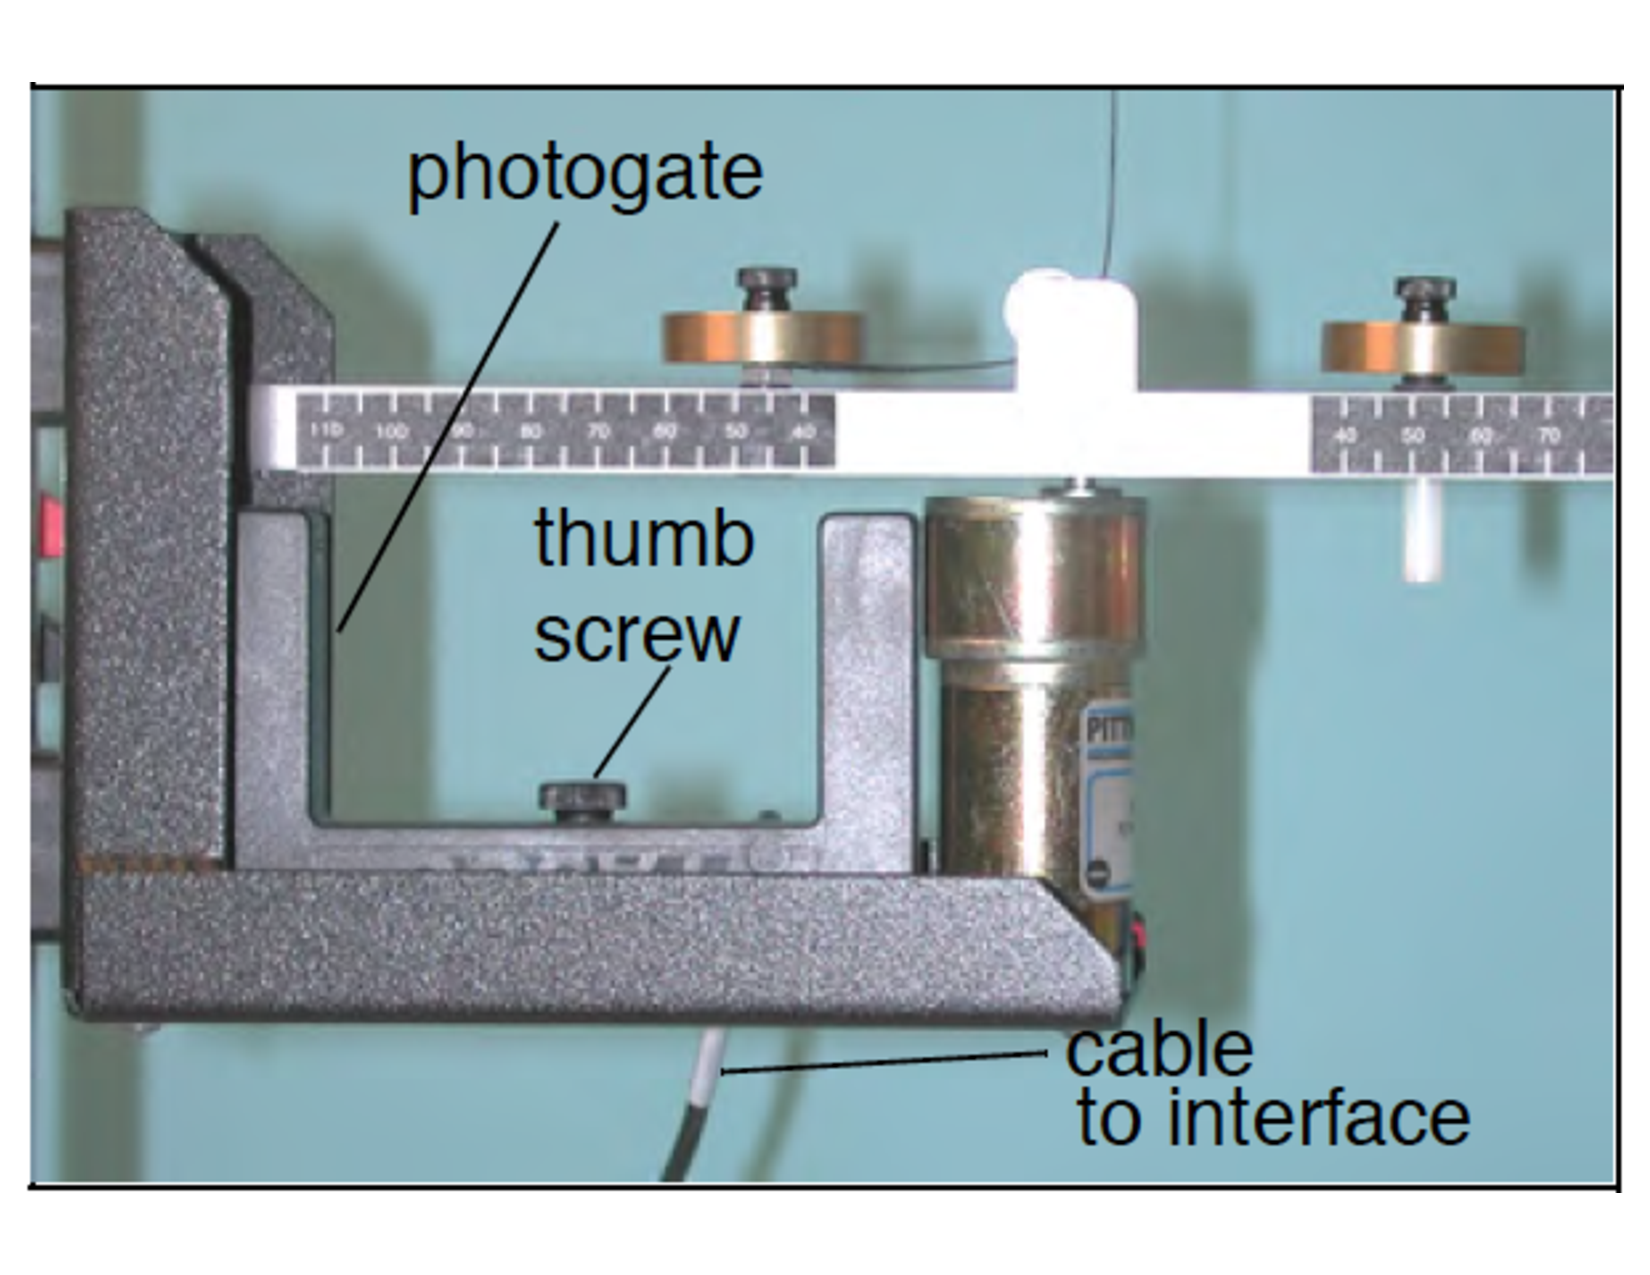
\includegraphics[width=2.9in]{Experiment08Figures/Figure01a.pdf}
    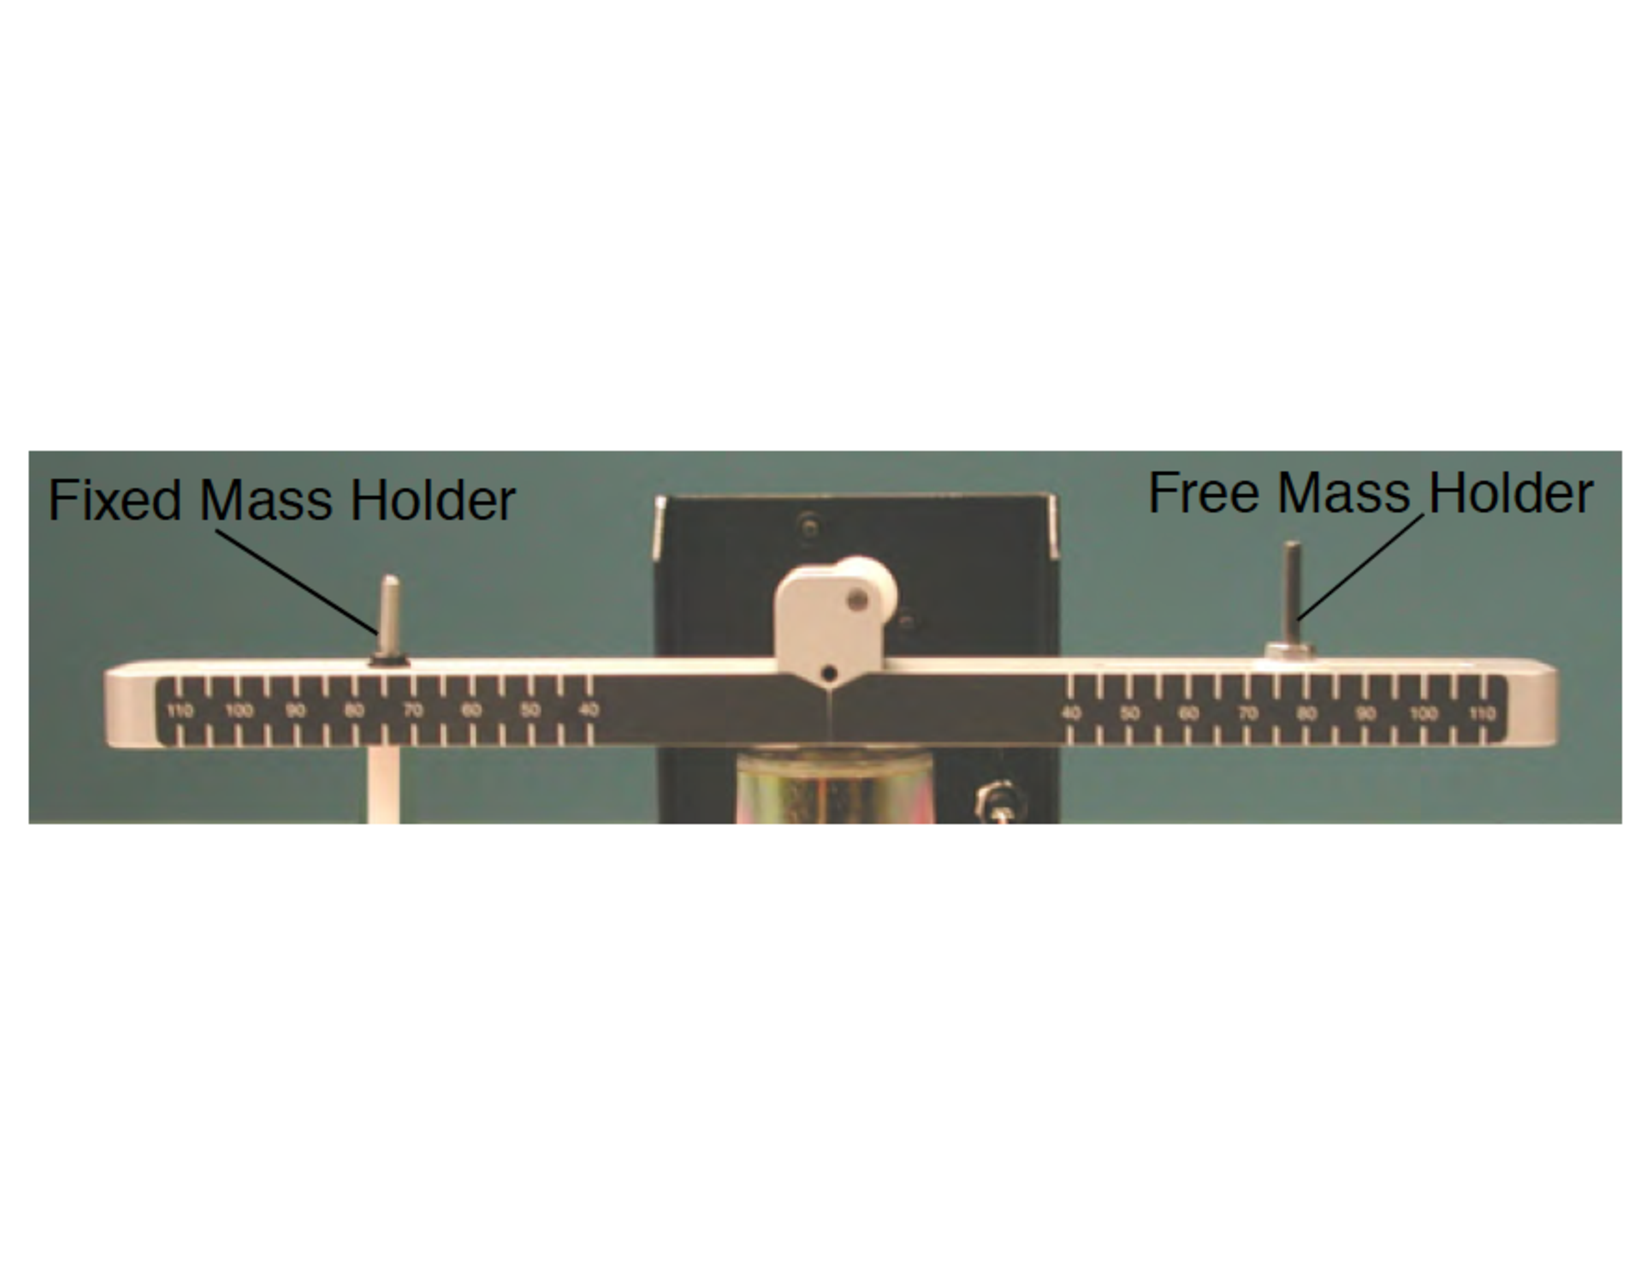
\includegraphics[width=2.9in]{Experiment08Figures/Figure01b.pdf}
  \end{center}
  \caption{Experimental Setup showing the rotating arm and the attached masses. The photogate to measure the speed is shown as well. The small white-ish pin attached underneath one of the mass holders is used to determine the speed $v$ of the mass.}
  \label{M04Fig01}  % the \label command comes AFTER the caption
\end{figure}

In order to determine $v$, the speed of the rotating mass, the rate at which the small pin attached underneath one of the two mass holders will move as it passes through the gap of the photogate is recorded. In order to do so correctly the width of the pin needs to be known to a very high precision.

In this experiment, the force needed to keep the mass at its predetermined radius is measured and plotted against the square of the speed of the mass at the same instant. You will repeat the experiment several times with different masses and at different radii.


\section{Experimental Procedure}

\begin{figure}
  \begin{center}
    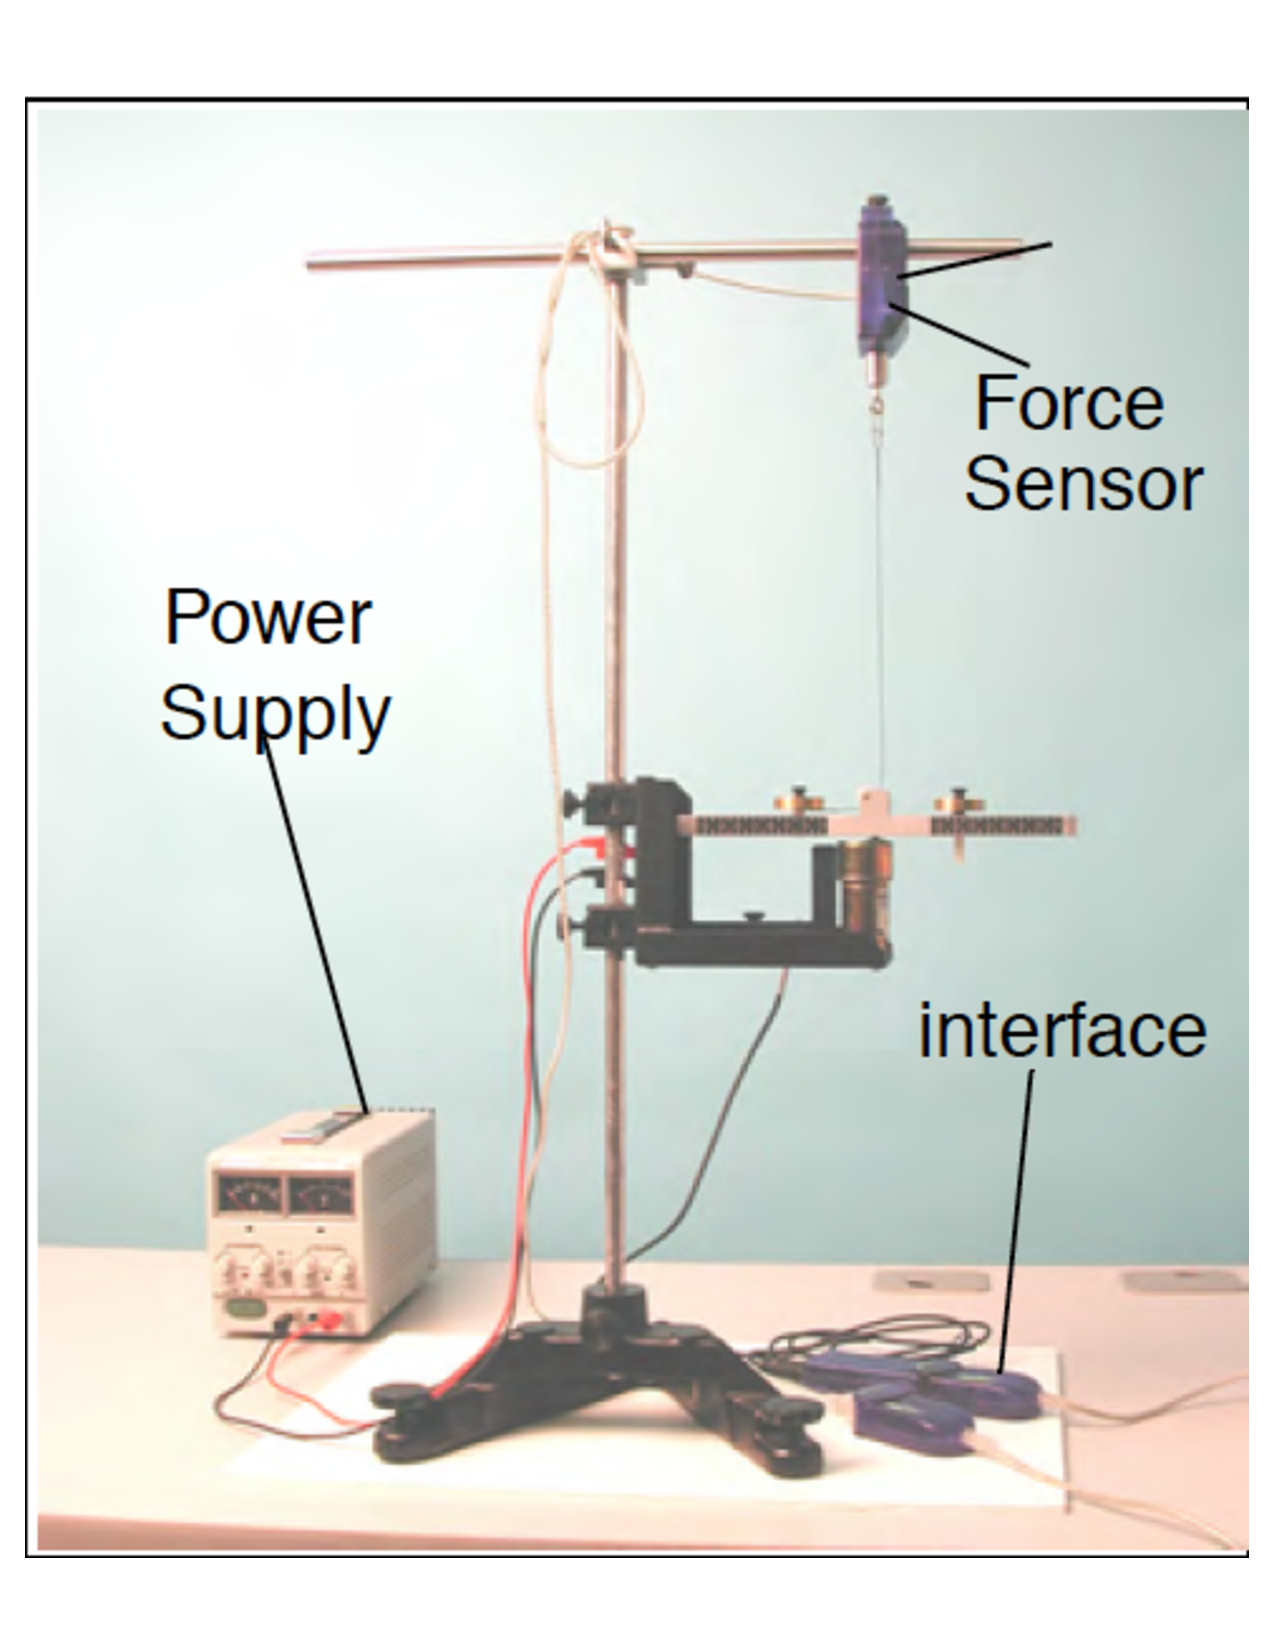
\includegraphics[width=2.6in]{Experiment08Figures/Figure02.pdf}
  \end{center}
  \caption{Experimental Setup for M-\ref{lab:M4}}
  \label{M04Fig02}
\end{figure}

\begin{figure}
  \begin{center}
    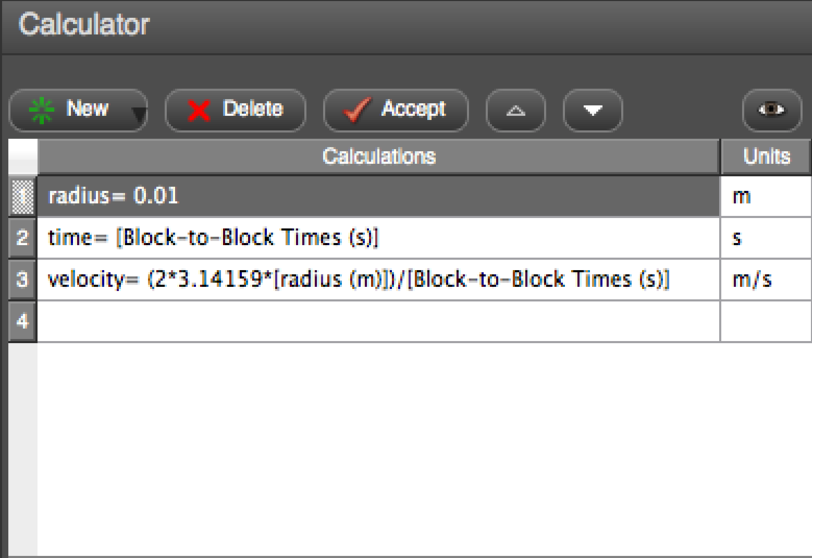
\includegraphics[width=3.3in]{Experiment08Figures/Figure03.pdf}
  \end{center}
  \caption{Setup of the data acquisition system \textbf{Capstone} to measure the speed of the rotating masses. Make sure to adjust the value for the radius in this window to the actual value used in your experimental setup.}
  \label{M04Fig03}
\end{figure}


\begin{itemize}
\item You'll run 6 cases, each with 3 trials:
\begin{itemize}
    \item 2 radii: short, long
    \item 3 different applied masses: 0 g (empty holder), 5 g, 15 g
\end{itemize}

\item[$\triangleright$] The experiment should already be setup for you as shown in Fig.~\ref{M04Fig02} with masses attached to both the fixed and free mass holders. %The force sensor should be  plugged into the computer via a PasPort adapter that connects a USB port on the computer. The photogate should be connected to a digital converter (a rectangular blue box), which has a USB connector on the other end. The USB connector should be connected to the computer.

\item Remove the free mass holder, and measure its mass with a triple-beam balance. Record this in your data sheet. Put the free mass holder back on the rotating arm.

  
%\item[$\triangleright$] Before you start you therefore need to set a few parameters in the \textbf{Capstone} data acquisition system on the computer. %See the page~\ref{sec:SettingUpHardware} for guidance.
%\item[$\triangleright$] Select \textbf{Hardware Setup} in the menu on the left-hand side on the \textbf{Capstone} interface. You should have an image of PasPort connector and the digital converter appear. Leave the PasPort connector alone --- \textbf{Capstone} will set this sensor up on its own.
%\item[$\triangleright$] With the mouse click on one of the two black dots on the image of the digital converter and select the photogate.
%\item[$\triangleright$] Once you have the photogate appear in the image, click on \textbf{Timer Setup}. The program will now guide you through the steps to set up the sensor.
%  \begin{itemize}
%  \item Step 1: Choose \textbf{Pre-configured timer}. Click \textbf{Next}.
%  \item Step 2: Make sure that the photogate is selected with a check mark. Click \textbf{Next}.
%  \item Step 3: Choose the option \textbf{Photogate with Pulley}. Click \textbf{Next}.
%  \item Step 4: Select only \textbf{Block-to-Block Times}. If any other options have a check-marked box, de-selected these options. Click \textbf{Next}.
%  \item Step 5: Leave the defaults ($\mbox{Spoke Arc Length} = 0.015\,\meter$ and $\mbox{Spoke Angle} = 36\degree$) for the two fields. Click %\textbf{Next}.
%  \item Step 6: You may leave the default name of the timer. Click \textbf{Finish}.
%  \end{itemize}
\item[$\triangleright$] Select \textbf{Calculator} in the menu on the left-hand side on the \textbf{Capstone} interface. This will open a window (example shown in Fig.~\ref{M04Fig03}) where you can update the radius to match the actual radius of your masses. \textit{NOTE}: that the value for the radius will change in the experiment, and you need to adjust the value in \textbf{Capstone} when you switch to the new radius.
  
%\item[$\triangleright$] You are now ready to collect data. Close the setup window by clicking on the \textbf{Calculator} button again.

\item[$\triangleright$] After setting the radius in the calculator, close the setup window by clicking on the \textbf{Calculator} button again.
\item[$\triangleright$] There are graphs set up for you in \textbf{Capstone} plotting
\begin{itemize}
    \item $F$ versus $v^2$
    \item $F$ versus $v$
\end{itemize}
\item Before data recording starts
\begin{itemize}
    \item Zero the force sensor with the zero button (physically on the force sensor) while the connecting cable is slack
\end{itemize}
\item[$\triangleright$] Start the data acquisition on \textbf{Capstone} by pressing the \textbf{Record} button.
  You should notice that the program will start to record values.
\item[$\triangleright$] Slowly increase the voltage on the power supply from 0V to 10V over the course of about 30 seconds.
  The metal arm will start to rotate and you will notice the graphs display the data as it is collected.
  Do not exceed 10 V and turn off the data acquisition (by pressing the \textbf{Record} button again) \textbf{before} returning the power supply to zero.
\item[$\triangleright$] Once you have finished your run, fit a line to your $F$ vs. $v^2$ graph.
  Select the fit box.
  In the Curve Fit Editor, lock the intercept $b = 0$.
  Notice the change in $m$ when you lock $b$. Record the slope $m$ in the Data Table.
\item[$\triangleright$] Fit a Quadratic curve to your $F$ vs. $v$ graph.
  Fit the curve $F=A v^2$ by locking B and C to zero. Notice the change in A when you lock B and C.
  Discuss why B and C should be zero. Record A in the Data Table.
\item[$\triangleright$] Repeat the measurement two more times.
  Calculate the average fit parameters for the three runs.
\item[$\triangleright$] Determine $m$, the value of the rotating mass from both graphs and note the result in your data table.
  Explain how you determine the value from your data.
\item[$\triangleright$] Repeat the experiment with two more masses at the same radius $R$.
  Please call for help in setting up the experiment with the new settings.
  Note all results in your data table. Discuss already why you also need to adjust the mass on the fixed mass holder and not just on the free mass holder.
\item[$\triangleright$] Repeat the experiment with the same 3 masses as above at a different radius $R$.
  Note all results in the data table.
\end{itemize}

%\clearpage
\section{Data Analysis}

%\begin{enumerate}
In this experiment, you measure the centripetal force with two different radii and three different applied masses for a total of six cases.
Each case is repeated for three trials.
The curve fitting to determine the mass is performed with the \textbf{Capstone} program.

For each case, construct a table with a row for each trial including:
\begin{itemize}
\item[$\triangleright$] the radius
\item[$\triangleright$] the applied mass plus the mass of the holder as measured earlier
\item[$\triangleright$] fit parameter $A$ from the $F$ vs. $v^2$ (linear fit)
\item[$\triangleright$] the mass determined from the centripetal $F$ vs. $v^2$
\item[$\triangleright$] the difference between the applied mass plus holder and the determined mass from $F$ vs. $v^2$
\item[$\triangleright$] fit parameter $m$ from the $F$ vs. $v$ (quadratic fit)
\item[$\triangleright$] the mass determined from the centripetal $F$ vs. $v$
\item[$\triangleright$] the difference between the applied mass plus holder and the determined mass from $F$ vs. $v$
\item[$\triangleright$] your estimate of the uncertainty in the radius (i.e. $\text{radius} \pm \text{how much?}$)
\item[$\triangleright$] the uncertainty in the mass from the centripetal force due to your estimated radius uncertainty (\textit{Point to consider}: how much does the derived mass change if you change your value for radius in \textbf{Capstone calculator} by the amount of your estimated radius uncertainty?)
\end{itemize}

From the data collected in the six cases you ran, determine the values of the masses $m$, using the given value for the radius $R$, as well as the related uncertainties.

%\end{enumerate}

%\section{Interpretation of Results}
%\begin{itemize}
%\item[$\triangleright$] Give an explanation on why the masses you measured do not agree with the masses of the weights you attached to the free mass holder.
%\item[$\triangleright$] Discuss, first among yourselves and then with your lab instructor what quantity of the experiment you could determine from your data. For your final answer, give an average value of this quantity.
%\item[$\triangleright$] In your report you need to include an answer as to 
%\end{itemize}




% Interpretation of Results
\section{Post-Lab Submission --- Interpretation of Results}
\begin{itemize}
\item Make sure to submit your finalized data table (Excel sheet)
\item Do the graphs display the expected behavior?
\item Discuss your results. Do your experimentally determined masses $\pm$ uncertainty agree with the actual mass of the applied masses plus mass holder?
\item Discuss uncertainties (sources of, how do they affect your final mass values; what would have the largest affect?).
\item What is the precision of your equipment?
\item What are possible systematic errors for today's experiments?
\item Why there should be the same mass on the fixed mass holder as compared to the free mass holder?
\end{itemize}







\newpage
\text{ }
%%%%%%%%%%%%%%%%%%%%%
%                                              %
%                 Experiment M-5               %
%            Conservation of Energy            %
%                                              %
%%%%%%%%%%%%%%%%%%%%%

\labChapter{M}{Conservation of Energy with Glider on Tilted Air Track}
\label{lab:M5}

% Introduction
%\section{Introduction}
% Background
\section{Background}

\textbf{Energy cannot be created nor destroyed.}  All that can really happen is a change in its form. We shall consider the conservation of mechanical energy, in particular, the sum of the kinetic energy and potential energy of a mass.  The kinetic energy is due to the motion of the mass and the potential energy is due to the relative position of the mass in the earth's gravitational field.  This total mechanical energy can only change if nonconservative forces are acting on any part of the system.  We will examine the exchange of kinetic and potential energy and the conservation of mechanical energy under the presumption of no nonconservative forces acting.  If the mechanical energy is not conserved we will attempt to determine potential sources of nonconservative work being done that would change the mechanical energy.





The \textbf{work} done by a force acting on a mass is the magnitude of the force acting in the direction of motion times the distance the mass moves.  Work is only done when the mass moves.  (In other words, you can push as hard as you like on a brick wall, but if the wall doesn't move, you didn't do any work!)  Assume for the moment that we have a mass $m$ moving on a frictionless, horizontal surface.  Assume a force acts on the mass from the position $x = 0$ to $x = x_1$ as illustrated in Fig.~\ref{M05Fig01}.  At position $x = 0$ it is moving with a velocity $v_{0}$ and at $x = x_1$ the velocity is $v_1$.

\begin{figure}
  \begin{center}
    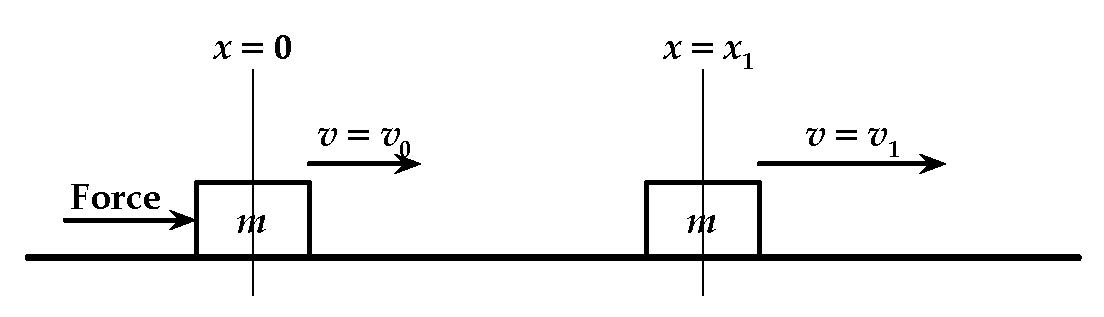
\includegraphics[width=5.0in]{Experiment04Figures/Figure01.pdf}
  \end{center}
  \caption{Explanation of the variables needed to calculate the amount of work done on a mass}
  \label{M05Fig01}  % the \label command comes AFTER the caption
\end{figure}

The work done by the force is $W_F = \vec{F} \cdot \vec{x_1}$.  Using Newton's second law it can easily be shown that the work done by the force changes a quantity we call the \textsl{kinetic energy}, $K = \nicefrac{1}{2} m v^2$.  Using the example illustrated in Fig.~\ref{M05Fig01},
\[
\vec{F} \cdot (\vec{x}_1 - \vec{0}) =
\frac{1}{2} m \,{v_1}^2 -  \frac{1}{2} m \,{v_0}^{2}.
\]
In this case, the force is acting in the direction of the motion and thereby increases the kinetic energy.  If the force were acting in the direction opposite to the motion, then the kinetic energy would be decreased.  If friction were present, it would act in the direction opposite to the direction of motion and thereby reduce the kinetic energy.  In this simple analysis, we have made no assumption as to the nature of the force.

A force like friction is a non-conservative force.  The work done by it not only depends upon the path the mass takes but is also not completely recoverable.  However, the work done on a mass by a conservative force can be completely returned to the mass as mechanical energy.  Thus work done by a conservative force can be represented by a potential energy function and depends only on the end points of the process. The gravitational force is a conservative force and is assumed constant in the vicinity of the surface of the earth.  The potential energy function is merely the work done by gravity on the way up or the way down and is equal to the gravitational force (the weight $m g$) times the change in height, $h$.  The gravitational potential energy, $U$, is given by
\[
U = m g h.
\]
The work done by this conservative force, like all conservative forces, only depends on the end-points of the path.  The gravitational potential energy is a relative quantity, i.e.\ it is a change in energy because of a change in elevation.  Thus we can choose a zero level arbitrarily.

If there are no non-conservative forces acting, then a mass moving only under the influence of gravity merely exchanges its kinetic and potential energy while the total energy remains constant.  For a mass stationary at some height, $h$, above the ground, all of its energy is potential energy of value $mgh$ with respect to the ground.  As the mass begins to fall under the influence of gravity, it loses $U$ and gains $K$  When it reaches the ground, the $U$ is zero with respect to the ground and the $K$ is a maximum, equal to the original $U$ at the top.  If the mass were a roller coaster, the coaster could climb back up to its original height where all the energy would be $U$ at which point it would momentarily stop, i.e.\ no $K$.  This assumes that neither friction nor any other nonconservative force is acting.  In general, we have
\[
\mbox{Work done by non-conservative Forces} = W_{N.C.} = \Delta K + \Delta U.
\]
If there are no non-conservative forces acting, then
\[
\Delta K + \Delta U = 0.
\]

In this experiment, we will use an air track to provide a nearly frictionless surface.  The track will be tilted at a measurable angle.  A glider will be released from rest at the top of the track and allowed to slide down and collide with a spring at the bottom. If the force of the spring on the glider is conservative, then the kinetic energy of the glider at the bottom is converted to potential energy in the compressed spring.  This potential energy is given back to the glider in the form of kinetic energy as the spring expands.  The glider bounces off and goes back up the track to its original height where the energy is again all $U$. If no energy is lost in the collision at the bottom, we say that the collision is completely elastic, implying that the forces involved in the collision are conservative.  After the collision, the glider will rebound up the track.  Getting back to its original height therefore implies no mechanical energy is lost during the entire path.  If it does not, we have to look for an energy loss mechanism and some non-conservative forces acting.

The change in height from the top to the bottom is measured allowing the change in $U$ to be calculated.  We will set the zero level for the potential energy at the bottom of track, at the position, $s_0$, in Fig.~\ref{M05Fig02}.

A measurement of the transit time from the top to the bottom will allow the calculation of the velocity at the bottom and therefore the $K$ at the bottom.  Finally, measuring the maximum height achieved on the rebound will yield a second value of $U$

The $K$ at the bottom of the track can be determined by measuring the average velocity from the release point at the top, $s_1$, to the collision point at the bottom, $s_0$, and then using Equation 1.  From a measurement of the transit time from $s_1$ to $s_0$, the velocity of the glider at the moment of collision at the bottom, $v_b$, can be determined by using the definition of average velocity, $v_{avg}$, thus:
\[
\frac{\Delta s}{\Delta t}  = v_{\mbox{avg}} = \frac{1}{2} (v_{b}+v_1)
\]
where the initial velocity, $v_1 = 0$, $\Delta s$ is the distance traveled down the track, and $\Delta t$ is the transit time of travel.

Rearranging terms we have the velocity at the bottom in terms of measurable quantities
\begin{equation}
  v_b = 2 v_{\mbox{avg}} = 2 (\Delta s / \Delta t).
\end{equation}
Using the definition of $K$, the $K$ at the bottom is then
\begin{equation}
  K_b = \frac{1}{2} m\, {v_b}^2.
\end{equation}

In order to calculate the potential energy, $U$ at any point, along the track we must determine the change in height between $s_1$ and $s_0$.  The potential energy at any position along the track is measured with respect to the collision point at the bottom, $s_0$, which is arbitrarily assigned a value of zero potential energy.  The $U$ is given by the weight of the glider, $mg$, times the change in vertical height.

Fig.~\ref{M05Fig02} is a simplified diagram of the inclined track. The distance $s$ is measured along the track by the scale attached to the side of the track.  The change in elevation, $\Delta h$, of any other point $s$ along the track can now be determined from the distance $s$ and the incline angle of track, $\theta$.  The incline of the track is produced by placing a spacer of known height under a leg at one end.  With the height of the spacer and the distance between the legs, $D$, the angle can be calculated (See Fig.~\ref{M05Fig03}).

\begin{figure}
  \begin{center}
    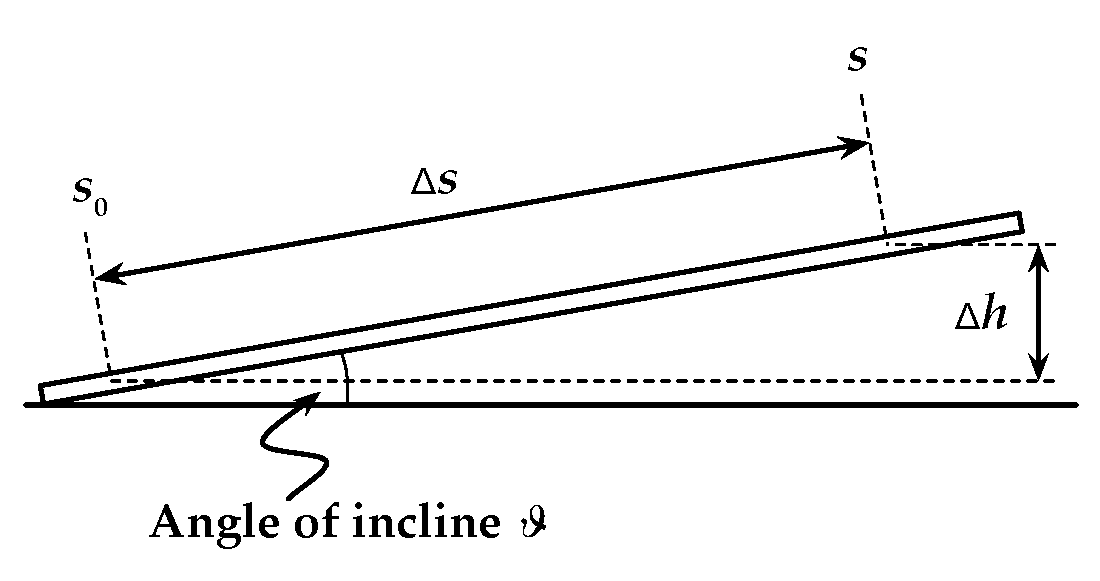
\includegraphics[width=4.5in]{Experiment04Figures/Figure02.pdf}
  \end{center}
  \caption{Schematic Drawing explaining the relationship between the track election $\Delta h$ and the distance $\Delta s$ for Experiment M-\ref{lab:M5}.}
  \label{M05Fig02}
\end{figure}

At $s_0$, $U_{b} = 0$, therefore $U_{s} = mg\, \Delta h = mg\, \Delta s \sin(\theta)$.
Referring to Fig.~\ref{M05Fig03}, the $\tan(\theta) = (\mbox{height of the spacer}) / (\mbox{distance between legs})$ or
\[
\tan(\theta) = \frac{H}{D}.
\]
With the very small angles of incline being used, we can safely assume that
\[
\tan(\theta) \sim \sin(\theta),
\]
therefore the potential energy, $U$, at some position, $s$, along the track is finally given by measurable quantities as
\begin{equation}
  U_s = mg \, \Delta s \frac{H}{D}.
\end{equation}

% Testing your Understanding
\section{Experimental Procedure}

\begin{figure}
  \begin{center}
    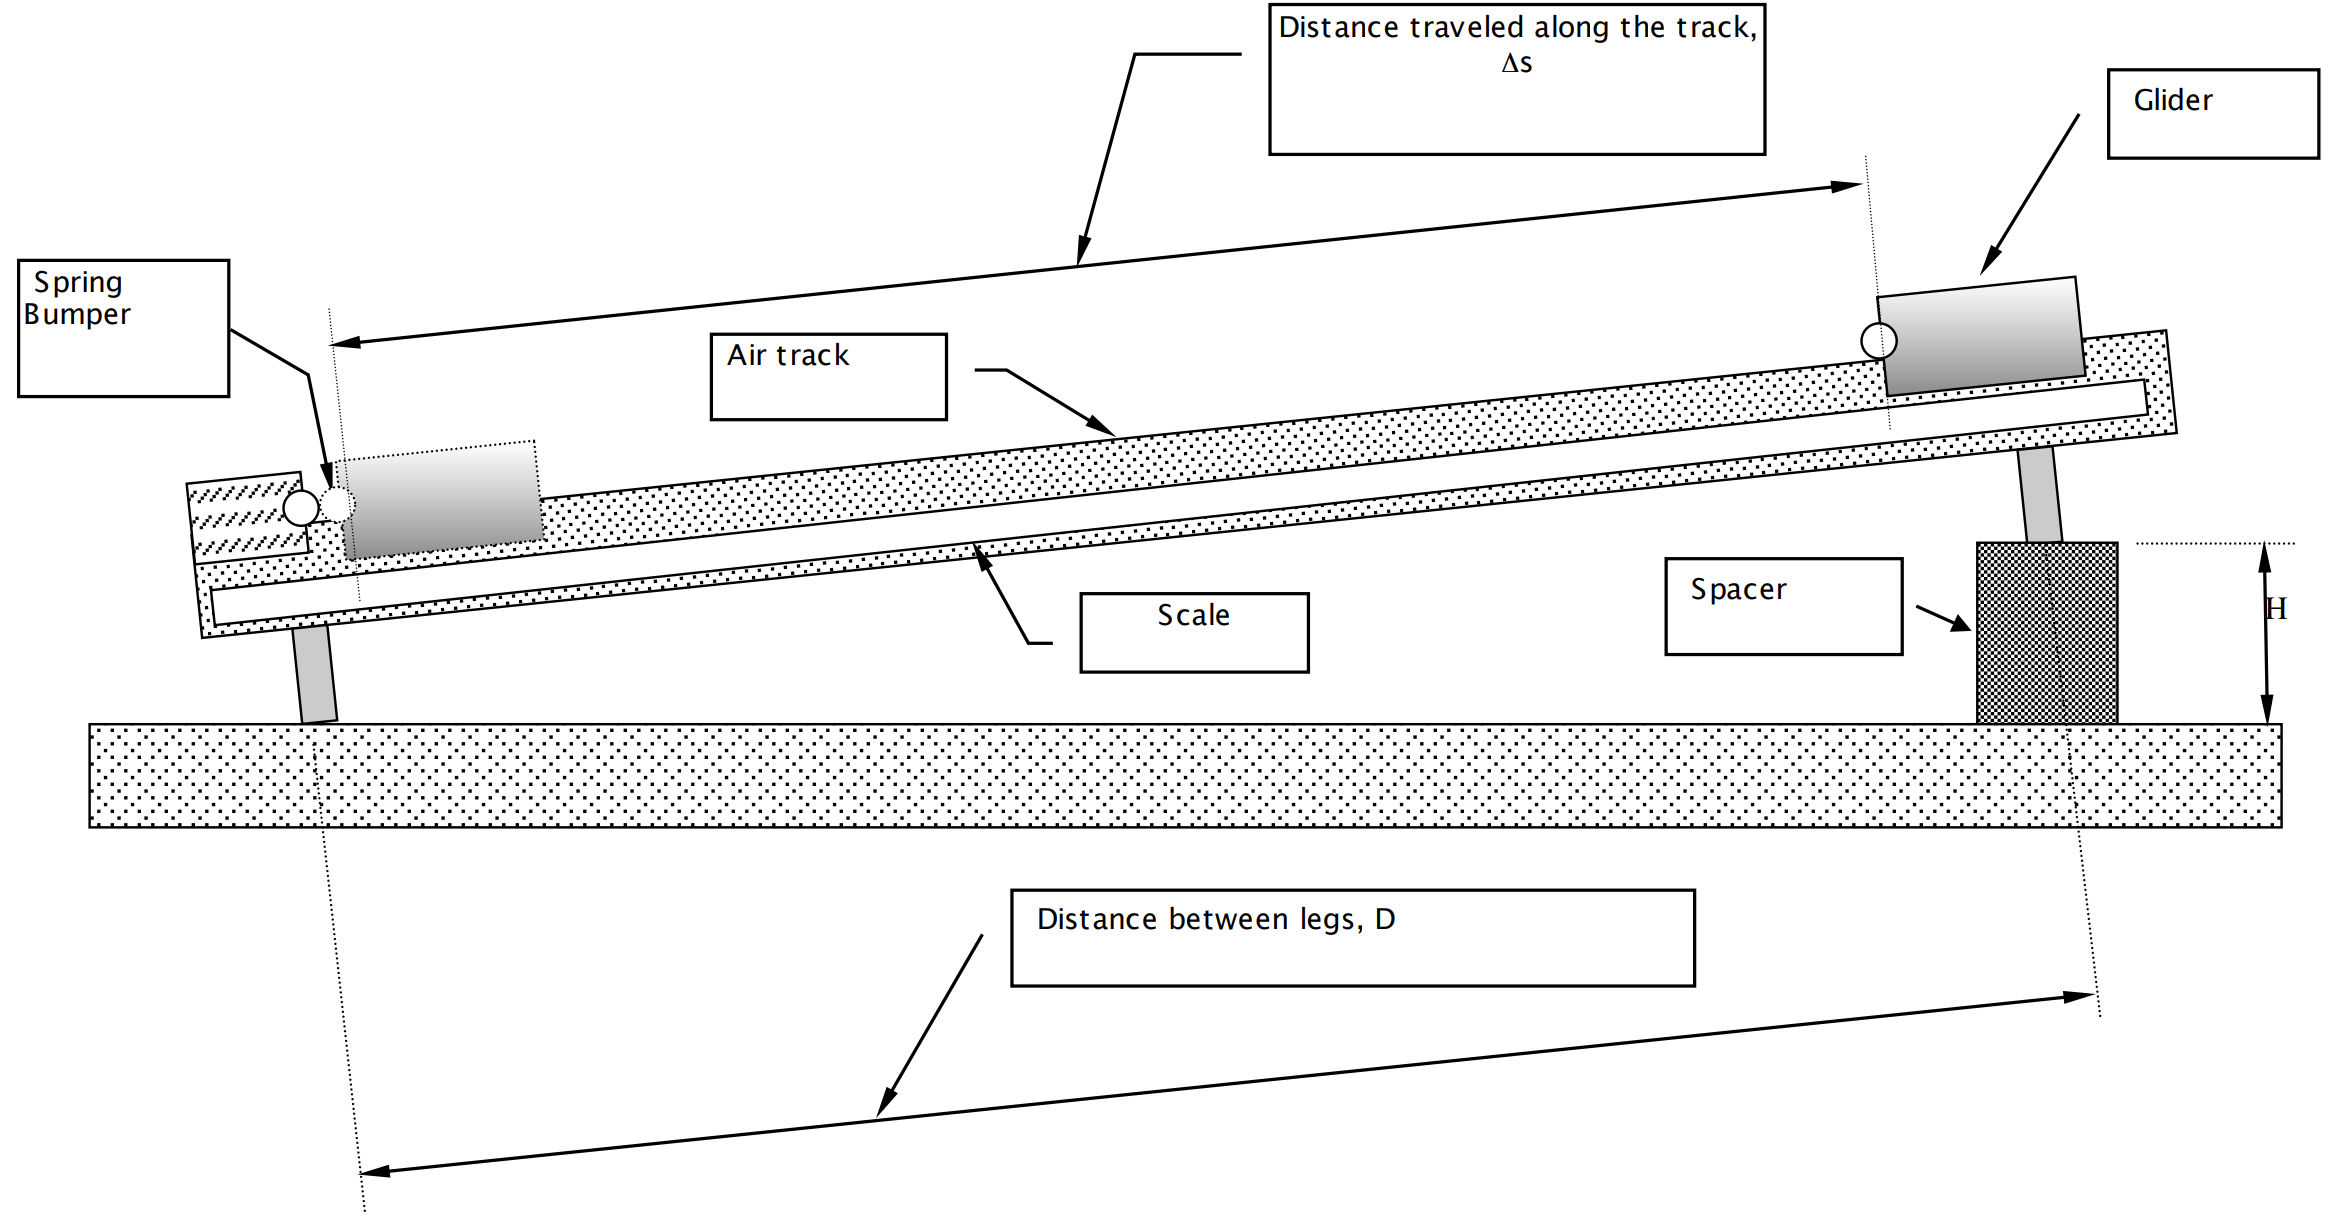
\includegraphics[width=5.8in]{Fall/Experiment04Figures/M04_fig2.png}
  \end{center}
  \caption{Experimental setup for Experiment M-\ref{lab:M5}.}
  \label{M05Fig03}
\end{figure}

\begin{itemize}
\item[$\triangleright$] Turn on the air and allow it to run a couple of minutes before proceeding.  It is very important that the track is clean and free of dirt.  This will prevent any damage to the very expensive air track and will keep friction to an absolute minimum.  Do not put a glider on the track without air flowing.
\item[$\triangleright$] Measure and record the mass of both a large and a small glider.
\item[$\triangleright$] Without the spacer present and the air track resting directly on the tabletop, place one of the gliders on the track and note any preferential drift of the glider.  Adjust the height of the single leg until the air track is level, as indicated by no preferential drift.  Check both orientations of the glider on the track to check if the car is asymmetric and has a significant preferential drift on an otherwise level track.  If this occurs, use another glider.
\item[$\triangleright$] Measure and record the distance $D$.  This is the center-to-center distance between the legs.
\item[$\triangleright$] Measure and record the heights $H$, of each of the two spacers.  Use a Vernier caliper for maximum accuracy. See the instructions at Fig.~\ref{VernierFig02} for using the Vernier caliper.
\item[$\triangleright$] Four cases will be performed, two gliders for two spacers.  Determine a convenient point on the glider to use with the scale attached on the side of track.  It doesn't matter what point you choose, only that you use the same point for all $s$ determinations for that glider.  A convenient point is the lower front or rear corner of the glider since it will be very close to the scale.
\item[$\triangleright$] For each case, perform the following steps and record the data appropriately in your spreadsheet:
  \begin{enumerate}
  \item Raise the single leg side of the track by placing a spacer under the knob.
  \item Place the glider at the bottom of the track resting against the bumper. Record $s_0$. (Note: With the car at this position, the red light on the bottom photogate should be lit. Moving the glider to the right the slightest distance should put the light out. If this is not the case, adjust the position of the photogate.)
  \item Next, place the glider near the top of the track. Move it slowly as you approach the top photogate. Stop the glider at the exact location when the red light comes on. Record $s_1$.
  \item Before you take the recorded data in the next step, take some practice runs. Your subsequent data will be much improved by your training!  %Set the photogate timer to pulse mode. 
  \begin{itemize}
      \item Position the glider so it is blocking the top photogate and the red light is on. Place one finger on the track in front of the glider and gently push the glider to the right until the red light on the photogate just goes out.
      \item Press record in \textbf{Capstone} to start the timer. \textit{NOTE: }\textbf{Capstone} may take a few seconds to start displaying times, once it's going, it will display the time whenever a photogate beam is broken; the time at the higher (start) photogate $t_1$ as well as the time at the lower (end) photogate $t_0$. Total transit time $\Delta t$ will be the the difference of the start and end times.
      \item Release the glider by quickly pulling your finger away from the track. After the glider bounces off the lower bumper, you can calculate the time of travel from top to bottom $\Delta t$.
  \end{itemize} 
    \item For each of the five trials, release the glider from the $s_1$ point and measure and record the following:
    \begin{itemize}
    \item The transit time $\Delta t$ from release at the top to the collision at the bottom.  Release the glider very carefully to insure that the initial velocity is zero.
    \item Allowing the glider to rebound off the bumper, record the rebound position $s_2$.  As the glider slows to a stop, capture the glider by gently pressing your finger near a lower corner of the glider just as it comes to a stop and then read $s_2$ off the scale.  Use the same point on the glider to read $s_2$ that you used to read $s_1$ and $s_0$.
    \end{itemize}
  \end{enumerate}
\end {itemize}

\textbf{Data Table:}

\begin{itemize}
\item[$\triangleright$] Create a table of the common data including the masses of the gliders, the distance $D$ between the legs of the air track and the heights of the two spacers.

\item[$\triangleright$] Create a table for each case with rows for each of the five trials including:
  \begin{itemize}
  \item The starting point $s_1$ at the top
  \item The stopping point $s_0$ at the bottom
  \item Start time at the top $t_1$
  \item End time at the bottom $t_0$
  \item The time $\Delta t$ (s) for each of the five trials
  \item The rebound position $s_2$ at the top
  \item Initial distance, $\Delta s_1=s_1-s_0$
  \item Initial potential energy at top, $U_{\mbox{top}}$
  \item The speed at the bottom, $v_{\mbox{b}}$
  \item Kinetic energy at the bottom, $K_{\mbox{b}}$
  \item Final distance, $\Delta s_2=s_2-s_0$
  \item Final potential energy at the rebound position, $U_{\mbox{rebound}}$
  \end{itemize}


\item[$\triangleright$] Create a summary table of the analysis with a row for each case including the following data:
  \begin{itemize}
  \item The average and standard deviation of the time, $\Delta t$, for the five trials
  \item The average and standard deviation of the speed at the bottom, $v_{\mbox{b}}$
  \item The average and standard deviation of the kinetic energy at the bottom, $K_{\mbox{b}}$
  \item The average and standard deviation of the final potential energy at the rebound position, $U_{\mbox{rebound}}$
  \item \% change from initial potential energy to kinetic energy at the bottom
  \item \% change from initial potential energy to final potential energy
  \end{itemize}

Calculate the following:
\begin{itemize}
\item[$\triangleright$] For each case, calculate the initial potential energy at $s_1$. Average the transit times, $\Delta t$, and calculate the velocity $v_b$ and the $K_b$.
\item[$\triangleright$] For each case, average the rebound position, $s_2$. Using this averaged value, calculate the final $U_2$.
\item[$\triangleright$] Calculate the percent change in mechanical energy from the top to the bottom.
\item[$\triangleright$] Calculate the percent change in mechanical energy from the initial release point $s_1$ to the final rebound point $s_2$.
\end{itemize}

\end{itemize}




\section{Post-Lab Submission --- Interpretation of Results}


\begin{itemize}
    \item Make sure to submit your finalized data table (Excel sheet)
    \item Arguing your responses with your data $\pm$ standard deviation:
    \begin{itemize}
        \item Is energy conserved between top and bottom?
        \item Is energy conserved between top/bottom and rebound?
    \end{itemize}
    \item Why is there a difference in energy conservation between the top/bottom and top/bottom/rebound?
    \item Uncertainties: 
    \begin{itemize}
        \item What is the precision of your equipment?
        \item What are the effects of measured uncertainties on your determined energies?
        \item What are possible systematic errors for today's experiments?
        \item How could one gain energy between top and bottom?
    \end{itemize}
\end{itemize}



\newpage
\text{ }
%%%%%%%%%%%%%%%%%%%%%%%%%%%
%                                                          %
%                          Experiment M-6                  %
%          Ballistic Pendulum & Projectile Motion          %
%                                                          %
%%%%%%%%%%%%%%%%%%%%%%%%%%%

%\labChapter{M}{The Ballistic Pendulum and Projectile Motion}
\labChapter{M}{Conservation of Energy \& Linear Momentum with Ballistic Pendulum \& Projectile Motion}
\label{lab:M6}

% Introduction
%\section{Introduction}
% Background
\section{Background}

Conservation of energy and linear momentum will be used to measure the initial velocity of a projectile.  Two techniques will be employed.

In the first, a ballistic pendulum, a device designed to capture a projectile in an initially stationary pendulum, will be used.  The conservation principles are used to analyze the collision and the subsequent motion of the pendulum.  The completely inelastic collision associated with the capture of the projectile in the pendulum and the subsequent motion of the pendulum provide the data necessary for the determination of the initial velocity.

In the second technique, the measured parameters of the trajectory of a horizontally launched projectile are used to determine the initial velocity.  With the projectile moving in a free-fall trajectory, constant acceleration kinematics will be used to determine the initial velocity from measurements of the horizontal range and vertical drop.

In each case, the projectile will be launched with the same device allowing a comparison of the initial velocity determinations of the two techniques.




% Ballistic Pendulum
\subsection{Ballistic Pendulum}

The ballistic pendulum is so named because it was originally used to measure the velocity of high-speed projectiles such as bullets long before electric and electronic timers made the procedure unnecessary.  It remains, however, as a simple and demonstrative device for understanding the conservation principles of energy and momentum.  In analyzing the problem, the system will consist of the projectile and the more massive pendulum.  As illustrated in the left image in Fig.~\ref{M06Fig01}, before the collision, the projectile is in motion horizontally towards the stationary pendulum.  After the collision, the projectile is imbedded in the pendulum and the pendulum is moving along the arc as shown in the right image of Fig.~\ref{M06Fig01}.

\begin{figure}
  \begin{center}
    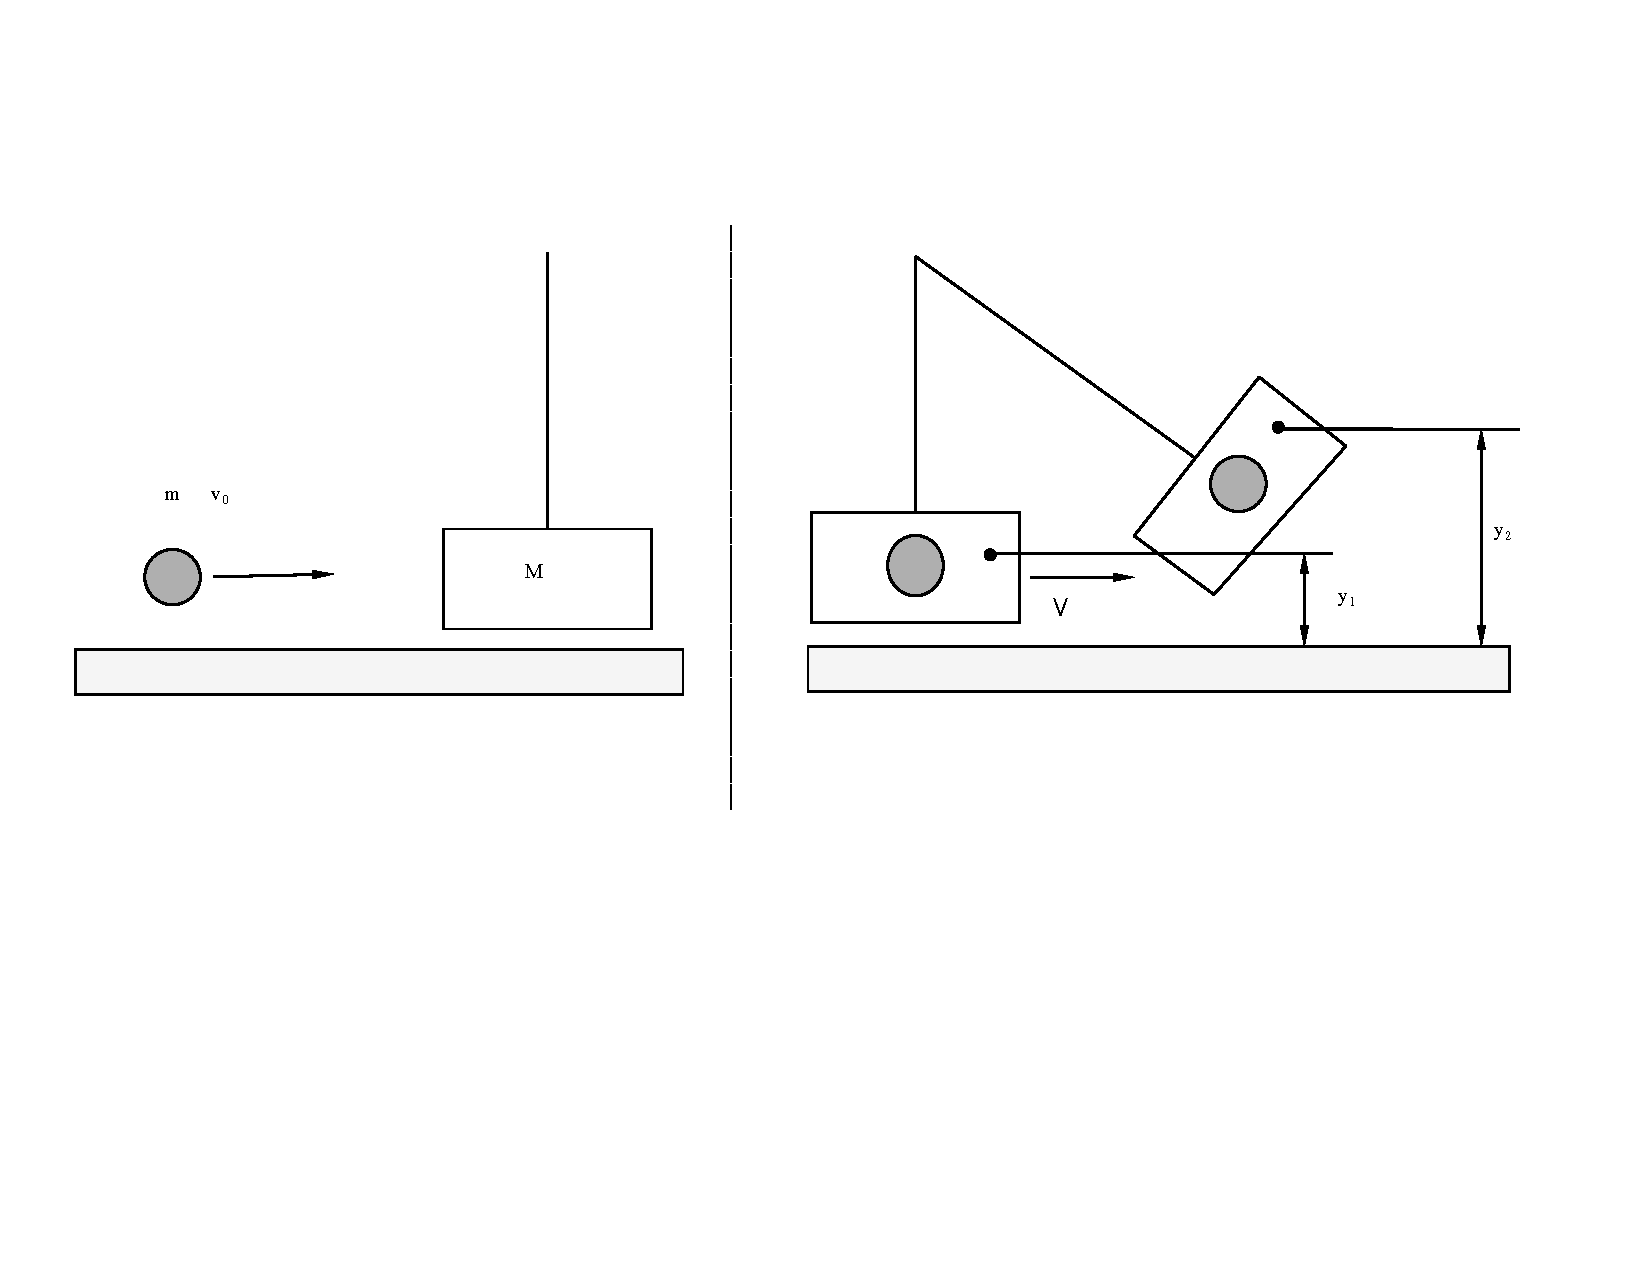
\includegraphics[width=5in]{Experiment05Figures/Figure01a.pdf}
  \end{center}
  \caption{Ballistic Pendulum before (left) and after the collision (right)}
  \label{M06Fig01}  % the \label command comes AFTER the caption
\end{figure}

The horizontally launched brass ball collides rather violently with and is captured by the more massive bob of the pendulum, initially at rest.  The violent collision is totally inelastic as the ball is captured by the pendulum with much of the initial kinetic energy of the ball lost through a variety of energy conversions, mostly heat.

During the collision of the ball with the pendulum, no external forces are acting on the system.  Newton's third law demands that the forces of the ball on the pendulum and the pendulum on the ball are equal and opposite.  These two, always equal and opposite, internal forces are acting for the same time and therefore produce equal and opposite impulses on the two bodies. Thus the change in momentum of one body is equal and opposite to the change in momentum of the other.  If the momentum changes of the two colliding bodies are equal and opposite, then the total linear momentum of the system cannot change and the total momentum is conserved.

Notice that there has been no assumption on the nature of the internal forces acting.  They do not have to be elastic, i.e.\ conservative.  As such, the conservation of momentum does not imply anything about the conservation of kinetic energy in the collision.  Linear momentum is conserved regardless of the nature of the interaction of the two bodies during the collision.  Only when the interactive forces are completely elastic, i.e.\ conservative, will the kinetic energy of the collision be conserved.

Momentum, like force and velocity, is a vector quantity.  The conservation of momentum of a system therefore implies the conservation of the total vector momentum of the system.  In our case, the initial momentum of the system is the initial momentum of the brass ball, which is only in the horizontal direction.  Therefore the momentum after the collision can only be in the horizontal direction and they must be equal.

Thus we can write
\begin{equation}
  \label{eq:M06momentum}
  m \vec{v}_0 = (m + M) \vec{V},
\end{equation}
where $m$ is the mass of the ball, $M$ is the mass of the pendulum, and $\vec{V}$ is the velocity of the pendulum and ball together.  If we can measure or determine $\vec{V}$, we can determine $\vec{v}_0$.  The determination of $\vec{V}$ can be made by examining the motion of the pendulum after the collision.

After the collision, the pendulum swings upward until it momentarily comes to rest at the top of its swing where the vertical height of the system has been increased from $y_1$ to $y_2$ (right image of Fig.~\ref{M06Fig01}).  We will now make some assumptions.  We will assume that there are no friction losses in the motion of the pendulum and that no collisions take place that might otherwise cause a loss of mechanical energy.  In other words, we are assuming that the total mechanical energy of the system is conserved after the collision.  By equating the kinetic energy of the system just after the collision at the bottom of the swing to the potential energy at the top, we can write
\[
\frac{1}{2}(m+M) V^2 = (m+M)  g \left(y_2 - y_1\right).
\]
Solving this expression for $V$ we have
\[
V = \sqrt{2 g \left(y_2 - y_1\right)}.
\]

Substituting in Eqn.~\ref{eq:M06momentum} above, we have finally an expression for the initial velocity of the ball in terms of the measurable change in height of the pendulum and the respective masses, i.e.
\begin{equation}
  \label{eq:M06v0} 
  v_0 = \left( \frac{m+M}{m} \right) \sqrt{2 g \left(y_2 - y_1\right)}.
\end{equation}

% Projectile Motion
\subsection{Projectile Motion}

When a projectile is moving solely under the influence of the force of gravity, we say that the projectile is in free-fall.  Consider the launching of the same ball used in the ballistic pendulum.  In this case, the pendulum will be swung up out of the way so the flight of the ball will continue off the edge of the table, eventually hitting the floor some distance away.  This situation is illustrated in Fig.~\ref{M06Fig02}.

\begin{figure}
  \begin{center}
    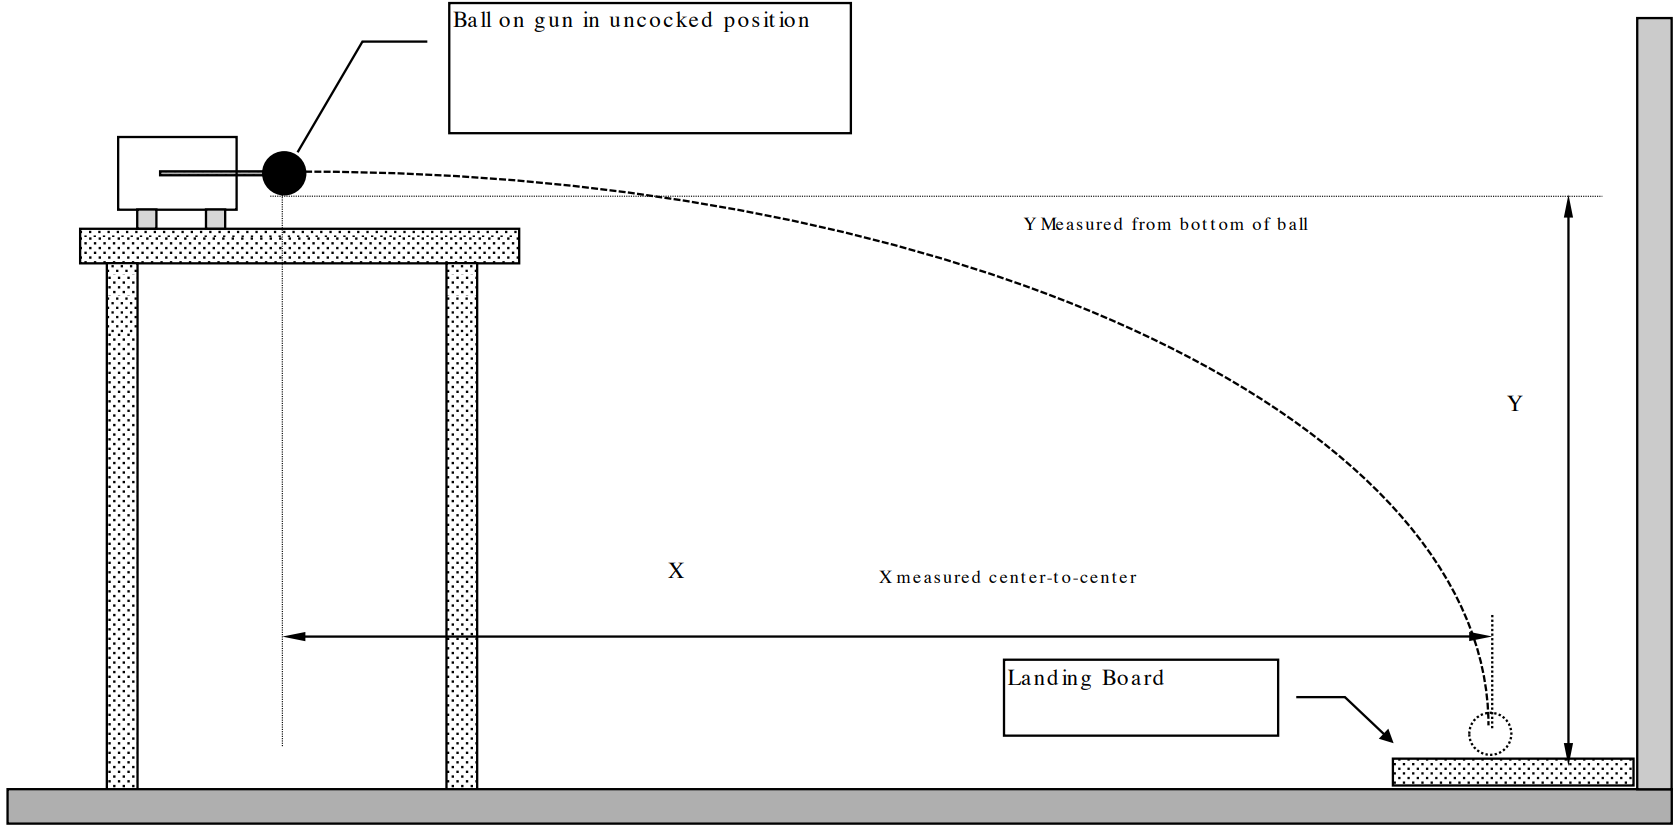
\includegraphics[width=6in]{Fall/Experiment05Figures/M06_fig02.png}
  \end{center}
  \caption{Projectile Motion}
  \label{M06Fig02}
\end{figure}

Once the ball leaves the spring gun used to launch the ball, the ball is in free-fall.  The vertical and horizontal motions are completely independent.  We assume that once the ball leaves the gun, there are no energy loss mechanisms during the flight of the ball.

In the vertical direction, the initial velocity is zero and the ball is accelerated downward by its weight, finally hitting the floor some time, $t$, later, dropping a vertical distance of $Y$.
In the horizontal direction, the ball has a constant velocity of $v_0$ during the entire flight over the horizontal distance $X$.

Using our kinematic expressions for constant acceleration motion, we have
\[
Y = \frac{1}{2} g t^2
\]
and
\[
X = v_0 \, t.
\]
Eliminating the time $t$ from these two expressions, we obtain
\begin{equation}
  \label{eq:M06v0pro}
  v_0 = X \sqrt{\frac{g}{2 Y}}.
\end{equation}


\section{Experimental Procedure}

% Ballistic Pendulum
\subsection{Ballistic Pendulum}

\begin{enumerate}
\item Data table:
\begin{itemize}
\item Create a table of the common data for the ballistic pendulum experiment including the mass of the ball $m$, the mass of the pendulum $M$, the initial pendulum height $y_1$ and any other common data needed for calculations.
\item Create a table with a row for each of the ten trials in the ballistic pendulum part of this lab including the trial number, %the rack number, 
the pendulum height $y_2$, the change in height $y_2-y_1$, the calculated velocity of the pendulum $V$, and the calculated initial velocity of the ball $v_0$.
\item Create a table to summarize the ten trials including the average pendulum height $y_2$, the average change in height $y_2-y_1$, the average velocity of the pendulum $V$, the average initial velocity of the ball $v_0$, the standard deviation of $v_0$.% and the standard deviation of the mean of $v_0$ using the methods in the Error Analysis section Eqns.~\ref{eq:errorSigmaX} and~\ref{eq:errorSigmaMeanX}.
\end{itemize}
\item Measure and record the mass of the brass ball projectile.
\item Record the mass of the pendulum that is indicated on the apparatus.
\item Practice the following procedure before actually taking data.
\item The pointer on the side of the bob indicates the center of mass of the pendulum.  With the pendulum hanging motionless, measure the height above the base plate of the pointer.  This value is $y_1$.   Record the value in meters.
\item Place the brass ball on the pin of the gun and press the ball so the spring of the gun is compressed until the trigger catches and holds the compressed spring.
\item Fire the gun by squeezing the trigger.  The ball will be captured by the bob and the pendulum will swing upwards.
\item A small ratchet engaging a rack will capture the maximum upswing position of the pendulum. % Note the value on the side of rack where the bob comes to rest and 
Measure the height to the tip of the metal pointer on the pendulum which represents the center of mass of the pendulum with ball.
\item Carefully release the ratchet so the pendulum can swing back to its equilibrium position.
\item Release the ball from the bob of the pendulum by pushing it with your finger or a short cylinder.  
\item Fire the ball ten times, and record the %rack number and 
pendulum height $y_2$ for each shot.
\item Calculate the average $y = y_2-y_1$ and the average $v_0$ from Eqn.~\ref{eq:M06v0}.
%\item Using the calculus method and assuming the error in $v_0$ comes from the variation in $y_2$, calculate the standard deviation
%  \begin{equation}
%    \label{eq:M06StandardDev}
%    \sigma(v_0) = \left(\frac{1}{2}\right)\frac{\bar{v}_0\, \sigma(y_2)}{\bar{y}_2 - y_1}.
%  \end{equation}
\item Record your data and calculations on your spreadsheet.
%\item You have multiple measurements that each give $v_0$. The average value is more precise than any individual measurement. The standard deviation of the mean value is less that the standard deviation of individual measurements. See Eqn.~\ref{eq:errorSigmaMeanX}. Your estimate of the error of the average of $n=10$ measurements is $\sigma(\bar{v}_0) = \sigma(v_0)/\sqrt{n-1}$ where $n=10$ is the number of measurements.


\end{enumerate}



% Projectile Motion
\subsection{Projectile Motion}

\begin{enumerate}
\item Data table:
\begin{itemize}
\item Create a table of the common data for the projectile motion experiment including the distance to the pad $x_1$, the vertical distance $Y$ and any other measurements.
\item Create a table with a row for each of the ten trials in the projectile motion part of this lab including the trial number, the measured $x_2$, the calculated horizontal distance $X=x_1+x_2$ and the calculated initial velocity of the ball $v_0$.
\item Create a table to summarize the ten trials including the average initial velocity $v_0$ of the ball, the standard deviation of $v_0$.% and the standard deviation of the mean of $v_0$.
\end{itemize}
\item Set up the projectile motion experiment as shown in Fig.~\ref{M06Fig02}.
\item Perform $n=10$ measurements of $x_2$. Be careful that the gun is in the same position for each measurement
\item Calculate the standard deviation for the $n=10$ measurements of $x_2$.
%\item Calculate the standard deviation for the velocity using the calculus method:
%\[
%  \sigma(v_0) = \bar{v}_0 \,\sigma(X) / \bar{X}
%\]
%where a bar over a symbol, as in $\bar{X}$, means the average value.
%\item Calculate the standard deviation of the mean of $v_0$.
\end{enumerate}



%\subsection{Comparing Projectile Motion and Ballistic Pendulum}
%The more measurements you make of a quantity, the better your estimate of the average value. The standard deviation of the mean is
%\[ \sigma(\bar{v}_0) = \frac{\sigma(v_0)}{\sqrt{n-1}}.\]
%Compare $\sigma(\bar{v}_0)$ from the projectile method and from the ballistic pendulum.  Which is larger? How do these numbers compare with the difference between $\bar{v}_0$ from the pendulum calculation and from the projectile calculation. If the difference of the two measurements is much larger than the standard deviation of the mean then you should suspect some systematic error. One possible systematic errors is an error in one of the other quantities which you measured only once. Another source of systematic error is some property of the apparatus that is not quite what you assumed.  What are some of the possible sources of systematic error in the two measurements?



\pagebreak

\section{Post-Lab Submission --- Interpretation of Results}

\begin{itemize}
    \item Make sure to submit your finalized data table (Excel sheet)
    \item What is the range of your measurements for both pendulum and projectile? Do the initial velocities agree within the ranges when treating your standard deviations as your uncertainty of average values?
    \item How and why are they (or could be) different.
   % \item The two results you found for $v_i$ are supposed to be the same value, since you used the same launching mechanism. 
    \item Which of the two results for the value of $v_i$ do you trust more? Explain your answer using a Physics argument.
    \item Suppose you would have used a more massive marble in the projectile motion portion of the experiment. How would this affect your result? Explain your answer.
    \item What are the effects of measured uncertainties on your determined velocities?
    \item What are possible systematic errors for today's experiments?
\end{itemize}



%Compare your standard deviations from the projectile method and from the ballistic pendulum. Which is larger? How do these numbers compare with the difference between $\bar{v}_0$ from the pendulum calculation and from the projectile calculation.


%Effect of uncertainties on your result?

%Compare $\sigma(\bar{v}_0)$ from the projectile method and from the ballistic pendulum.  Which is larger? How do these numbers compare with the difference between $\bar{v}_0$ from the pendulum calculation and from the projectile calculation.

%If the difference of the two measurements is much larger than the standard deviation of the mean then you should suspect some systematic error. One possible systematic errors is an error in one of the other quantities which you measured only once. Another source of systematic error is some property of the apparatus that is not quite what you assumed.  What are some of the possible sources of systematic error in the two measurements?



%%%%%%%%%%%%%%%%%%%%%%%%%
%                                                 %
%                 Experiment M-8                  %
%         Experiment Title  Rotational Motion     %
%                                                 %
%%%%%%%%%%%%%%%%%%%%%%%%%

%\labChapter{M}{[1171L] - Rotational Motion}
\labChapter{M}{[1171L - CALC-BASED course] --- Rotational Dynamics with Moment of Inertia \& Angular Momentum}
\label{lab:M7_1171L}

% Introduction
%\section{Introduction}
% Background
\section{Background}

The motion of an object can be divided into two, completely independent parts: the linear (translational) motion of the center of mass and the rotational motion of the object around an axis through the center of mass. The linear motion is explained by Newton's 2nd Law of motion: a net force $F_{net}$ acting on an object of mass $m$ will cause the object to experience a linear acceleration $a$ given by
\[
F_{net} = m a.
\]
Rotational motion can be described in a very similar manner, but the quantities involved need to be changed to rotational quantities. These quantities are described and explained in detail in the following paragraphs.



% Moment of Inertia
\subsection{Moment of Inertia}

In rotational motion the moment of inertia (usually denoted by $I$) takes the role of mass. An object with a large value of $I$ will be reluctant to change its rotational motion. Just as mass this quantity is a scalar, meaning that it has no direction. The moment of inertia of a system of objects can be determined easily by adding the moment of inertia of each of the different components making up the entire system. The moment of inertia depends not only on the mass of the object but also on how the mass is distributed with respect to the axis of rotation. The further the mass is away from the axis of rotation, the higher the moment of inertia will be. For a point mass (an object that can be considered small with respect to its distance from the axis of rotation) the moment of inertia is defined as
\begin{equation}
  \label{eq:M08pointMass}
  I = m\, R^{2}
\end{equation}
where $m$ is the mass of the object and $R$ is the distance of the object from the axis of rotation.
The calculation of the moment of inertia for more complex objects is a rather straightforward process, but can be very tedious. In most cases simple expressions can be found to calculate the value of $I$. The list below gives the moment of inertia for a few objects used in this lab:

\begin{itemize}
\item[$\triangleright$] A \textbf{solid disk} of mass $M_{D}$ and radius $R_{D}$ rotating about an axis through its center: 
  \begin{equation}
    \label{eq:M08Idisk}
    I= \frac{1}{2} M_{D} \, R_{D}^{2}
  \end{equation}
\item[$\triangleright$] A \textbf{thin-walled ring} of mass $M_{R}$ and radius $R_{R}$ rotating about an axis through its center: 
  \begin{equation}
    \label{eq:M08Ithinring}
    I= M_{R} \, R_{R}^{2}
  \end{equation}
\item[$\triangleright$] A \textbf{thick ring} mass $M_{R}$ and inner radius $R_{i}$ and outer radius $R_{o}$ rotating about an axis through its center:
  \begin{equation}
    \label{eq:M08Ithickring}
    I=\frac{1}{2} M_{R} \, \left(R_{i}^2 + R_{o}^2\right)
  \end{equation}
\end{itemize}

% Torque
\subsection{Torque}

A force by itself is not enough to determine whether an object will start to rotate (just think about how a force that is applied to the hinges of a door will not rotate the door). Instead we define a new quantity, called torque $\tau$, which combines the force and the distance from the axis of rotation (also called the lever arm). This quantity is a vector quantity, meaning that it does have a direction
\begin{equation}
  \vec{\tau} = \vec{F}_{\perp} \times \vec{d}.
\end{equation}
Here $\vec{d}$ denotes the lever arm (directed outward from the center) and $\vec{F}_{\perp}$ is the component of the force perpendicular to the lever arm.

% Newton's 2nd Law for Rotational Motion
\subsection{Newton's 2nd Law for Rotational Motion}

With the above definitions we can now formulate a rotational version of Newton's 2nd Law. An object with moment of inertia $I$ will experience an angular acceleration $\vec{\alpha}$, if a net torque $\vec{\tau}_{\mbox{net}}$ acts on it
\begin{equation}
  \vec{\tau}_{\mbox{net}} = I \vec{\alpha}.
\end{equation}


\pagebreak 
% Calculating the moment of inertia
\subsection{Calculating the Moment of Inertia}

One can use Newton's 2nd Law for Rotational Motion to calculate the moment of inertia of an object from the angular acceleration $\alpha$ and the net torque acting on the object.
\[
I = \frac{\left|\vec{\tau}_{\mbox{net}}\right|}{\left|\vec{\alpha}\right|}
\]



The simplified sketch in Fig.~\ref{M08Fig01} shows the setup used in this lab.
The net torque acting on the pulley can be written as
\[
|\vec{\tau}_{\mbox{net}}| = T \, R_{P}
\]
where $T$ is the tension in the string and $R_{P}$ is the radius of the 3-step pulley. Since the tension is not known it has to be determined from the linear acceleration a of the hanging mass, using the net force acting on the mass $m$ (see force diagram in the sketch):
\[
F_{\mbox{net}} = m g - T = m a.
\]
In addition the linear acceleration $a$ is related to the angular acceleration $\alpha$ by
\[
a = \alpha R_{P}.
\]

Using this set of equations one can now solve for the moment of inertia, $I$,
\begin{equation}
  \label{eq:M08Eq03}
  I = \frac{m \left(g  R_{P} - \alpha R_{P}^2\right)}{\alpha}.
\end{equation}


\begin{figure}
  \begin{center}[h]
    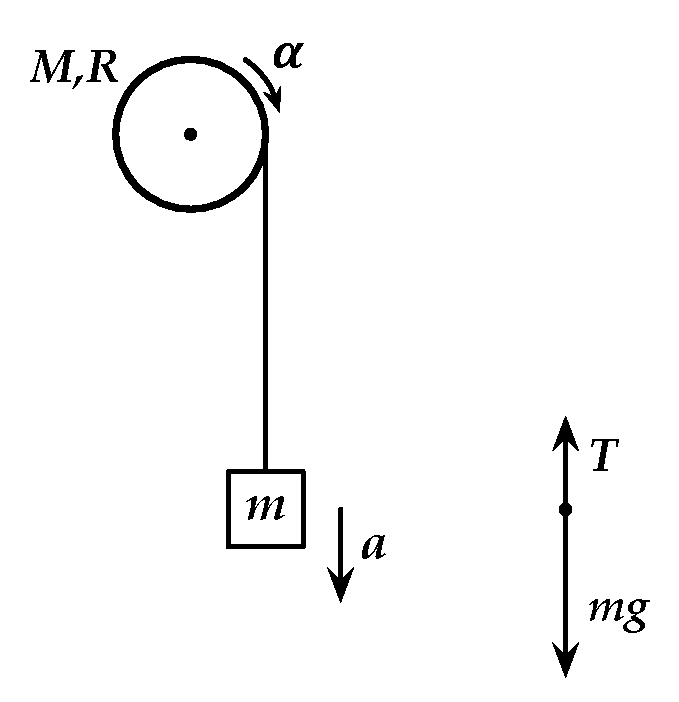
\includegraphics[width=2.2in]{Experiment09Figures/Figure01.pdf}
  \end{center}
  \caption{Left: Sketch of a pulley of mass $M$ and radius $R$ being accelerated by a hanging mass $m$. Note that the pulley in the lab is actually horizontal, but is drawn vertically here for simplicity. Right: Force diagram for the hanging mass $m$.}
  \label{M08Fig01}  % the \label command comes AFTER the caption
\end{figure}




% Angular Momentum
\subsection{Angular Momentum}

A similar derivation as above can be used to define the quantity of angular momentum $\vec{L}$ from the definition of linear momentum ($\vec{p} = m \vec{v}$)
\[
|L| = I \omega
\]
Angular momentum is conserved (meaning it will not change its value) if there is no external torque acting on a system
\[
\vec{L}_i = {L}_f.
\]
This can be used to determine the angular velocity of a system if the moment of inertia changes
\begin{equation}
  I_i \omega_i = I_f \omega_f.
\end{equation}


\textbf{THE PARALLEL AXIS THEOREM} is used to calculate the moment of inertia of an object of mass $M$ rotating about a rotation axis that does not pass through the center of mass (e.g. the ring on top of the apparatus is off center). The moment of inertia for the axis ${I_{axis}}$  is
\begin{equation}
\label{M7RotationalMotion_OffAxis}
    {I_{axis}} = {I_{ring}} + M d_{cm}^2
\end{equation}
where ${I_{cm}}$ is the moment of inertia about an axis through the center of mass parallel to the rotation axis. The distance between the parallel axes is ${d_{cm}}$. In the Conservation of Angular Momentum experiment you drop the ring on the rotating apparatus.  Although you try to drop the ring centered on the axis of rotation, it often lands off center. You will run a case where you try to center it, and then another case where you purposefully drop it off center.


\section{Experimental Procedure}

The experiment makes use of a sensor, which is able to detect and measure angular displacement, angular velocity, and angular acceleration. This Rotary Motion Sensor (RMS), with a \textbf{stated uncertainty of 0.09\degree}, is attached to a vertical rod and has a 3-step pulley affixed to its axle (see Fig.~\ref{M08Fig02}). Objects with different moment of inertia can be mounted onto the 3-step pulley and their rotational motion be measured. A second pulley (called a Super Pulley) is attached to the RMS to allow a string to spool off the 3-step pulley as shown in Figures~\ref{M08Fig02} and ~\ref{M08Fig03}. A weight hanger of known mass $m$ is attached to the free end of the string and provides an accelerating torque to the 3-step pulley and therefore to the object mounted on it.

In this experiment you will measure the angular acceleration from a graph of angular velocity vs. time using data recorded with the RMS. The data will be collected in \textbf{Capstone}, which also provides analysis tools. %See page~\ref{sec:SettingUpHardware} for guidance. 
The moment of inertia of a ring and of two point masses will be determined from the angular acceleration. Finally, you will verify the validity of angular momentum conservation in an inelastic collision.

\begin{figure}
  \begin{center}
    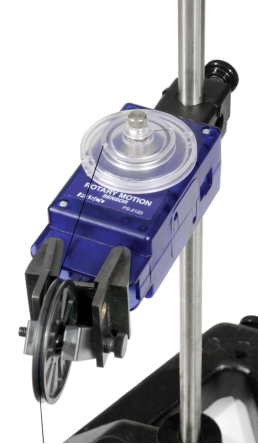
\includegraphics[width=2.2in]{Experiment09Figures/Figure02.pdf}
  \end{center}
  \caption{Rotary Motion Sensor (RMS) with 3-step pulley (transparent) and Super Pulley (black).}
  \label{M08Fig02}
\end{figure}

\begin{figure}
  \begin{center}
    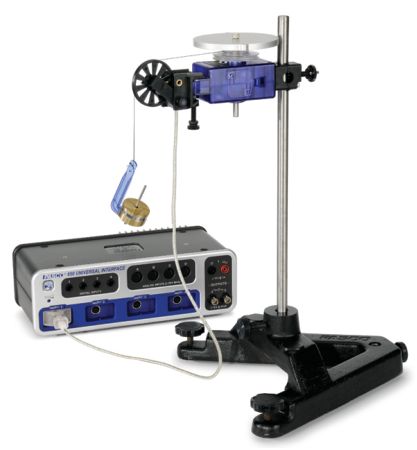
\includegraphics[width=2.4in]{Experiment09Figures/Figure03a.pdf}
    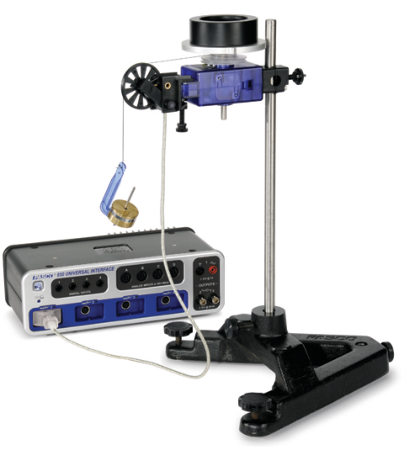
\includegraphics[width=2.4in]{Experiment09Figures/Figure03b.pdf}
  \end{center}
  \caption{Experimental setup of the RMS apparatus with disk alone (left) and with disk and ring mounted (right). The setup varies slightly from the one used in the lab.}
  \label{M08Fig03}
\end{figure}

% Moment of Inertia of the Ring
\subsection{Moment of Inertia of the Ring}

In Part~1 of the experiment you will measure the moment of inertia of the ring and of the apparatus by measuring angular acceleration with a known torque.
\begin{itemize}
\item[$\triangleright$] Create a Part~1 Data Table for your measurements and calculations of the moment of inertia of the ring.
\item[$\triangleright$] Determine the mass of the ring and note the result as $M_{\mbox{ring}}$ in your Part~1 Data Table.
\item[$\triangleright$] Measure the inner and outer radii of the ring, using the calipers. See the instructions at Fig.~\ref{VernierFig02} for using the Vernier caliper. Note the result as $R_{i}$ and $R_{o}$ in your Part~1 Data Table.
\item[$\triangleright$] Calculate the expected moment of inertia of the ring, using Eqn.~\ref{eq:M08Ithickring} given in the Background. Note your result as $I_{\mbox{calc}}$ in your Part~1 Data Table.
\item[$\triangleright$] Place the ring onto the disk, which should already be mounted on the Rotary Motion Sensor (RMS). The two pins of the ring should fit into the two holes on the disk.
\item[$\triangleright$] Note the mass of the hanger as $m$ in your Data Table.
\item[$\triangleright$] Using the calipers measure the radius $R_{P}$ of the smaller pulley of the RMS and note your result in your Part~1 Data Table. See the instructions at Fig.~\ref{VernierFig02} for using the Vernier caliper.
\item[$\triangleright$] Wind the string with the attached mass hanger onto the smaller pulley of the RMS. You need to make sure that the string runs over the Super Pulley, is wound nicely onto the smaller pulley of the RMS, and is leaving the pulley of the RMS tangentially before it runs straight over the Super Pulley.
\item[$\triangleright$] Measure the angular acceleration $\alpha_{\mbox{total}}$ of the ring plus the apparatus (the disk and the RMS).
  \begin{enumerate}
  \item Make sure that in \textbf{Capstone} you have a graph of angular velocity ($y$-axis) vs. time ($x$-axis) open.
  \item Before releasing the mass hanger press the \textbf{Record} button on \textbf{Capstone}.
  \item Release the mass hanger and note that the recorded graph is a straight line.
  \item Press the \textbf{Record} button again right before the string is completely unwound from the pulley to stop recording any more data points.
  \item Using the \textbf{Fit} option in \textbf{Capstone}, fit a straight line (linear fit) to the data, in the region where the system is accelerating (highlight the data region in the graph you want to fit).
  \item The slope of this graph is the angular acceleration $\alpha_{\mbox{total}}$.
  \item Note your result in your Data Table.
  \end{enumerate}
\item[$\triangleright$] Calculate the moment of inertia of the apparatus plus the ring, using Eqn.~\ref{eq:M08Eq03} given in the Introduction. Note your result as $I_{\mbox{total}}$ in your Part~1 Data Table.
\item[$\triangleright$] Remove the ring from the apparatus and repeat the above steps to determine the moment of inertia of the apparatus without the ring. Note the results as $\alpha_{\mbox{app}}$ and $I_{\mbox{app}}$ in your Data Table.
\item[$\triangleright$] To determine the moment of inertia of the ring subtract $I_{\mbox{app}}$ from $I_{\mbox{total}}$. Note your result as $I_{\mbox{exp}}$ in your Data Table.
\item[$\triangleright$] Repeat the above measurements three times.
\item[$\triangleright$] Calculate averages and standard deviations $\sigma(I)$ for the moments of inertia.% (See Eqn.~\ref{eq:errorSigmaX}).
\item[$\triangleright$] Compare the difference between your calculated value and the experimental value with its uncertainty.
\end{itemize}

% Moment of Inertia of two point masses
\subsection{Moment of Inertia of Two Point Masses}
In Part~2 of the experiment, you will measure the moment of inertia of two point masses on a rod. 
\begin{itemize}
\item[$\triangleright$] Create a Part~2 Data Table for your measurements and calculations of the moment of inertia of the point masses.
\item[$\triangleright$] Please call the lab instructor for this: Mount the rod onto the pulley of the RMS.
\item[$\triangleright$] Determine the masses of the two brass weights (with screws) and note the result as $M_1$ and $M_2$ in your Data Table.
\item[$\triangleright$] Mount the masses into the end of the rod and fasten them with the screws. Measure the distance of the center of the masses from the center of the rod. Note the results as $R_1$ and $R_2$ in your Data Table.
\item[$\triangleright$] Calculate the expected moment of inertia of the two points masses, using Eqn.~\ref{eq:M08pointMass} given in the Introduction. Note your result as $I_{\mbox{calc}}$ in your Data Table.
\item[$\triangleright$] Note the mass of the hanger as $m$ in your Data Table.
\item[$\triangleright$] Note the radius $R_{P}$ of the smaller pulley of the RMS in your Data Table (use the result from Part~1 above).
\item[$\triangleright$] Wind the string with the attached mass hanger onto the smaller pulley of the RMS. You need to make sure that the string runs over the Super Pulley, is wound nicely onto the smaller pulley of the RMS, and is leaving the pulley of the RMS tangentially before it runs straight over the Super Pulley.
\item[$\triangleright$] Measure the angular acceleration $\alpha_{\mbox{total}}$ of the two masses plus the apparatus (the rod and the RMS):
  \begin{enumerate}
  \item Make sure that in \textbf{Capstone} you have a graph of angular velocity ($y$-axis) vs. time ($x-axis$) open.
  \item Before releasing the mass hanger press the \textbf{Record} button on \textbf{Capstone}.
  \item Release the mass hanger and observe the recorded data points/graph.
  \item Press the \textbf{Record} button again right before the string is completely unwound from the pulley to stop recording any more data points.
  \item Discuss (among yourselves and with your instructor) the resulting graph before continuing.
  \item Using the \textbf{Fit} option in \textbf{Capstone}, fit a straight line (linear fit) to the data, in the region where the system is accelerating (highlight the data region in the graph you want to fit).
  \item The slope of this graph is the angular acceleration $\alpha_{\mbox{total}}$.
  \item Note your result in your Data Table.
  \end{enumerate}
\item[$\triangleright$] Calculate the moment of inertia of the apparatus plus the two point masses, using Eqn.~\ref{eq:M08Eq03} given in the Introduction. Note your result as $I_{\mbox{total}}$ in your Data Table.
\item[$\triangleright$] Remove the two point masses from the apparatus and repeat the above steps to determine the moment of inertia of the apparatus without the two masses. Note the result as $I_{\mbox{app}}$ in your Data Table. Please note that you need to again discuss the collected data points/graph with your lab instructor.
\item[$\triangleright$] To determine the moment of inertia of the two point masses subtract $I_{\mbox{app}}$ from $I_{\mbox{total}}$. Note your result as $I_{\mbox{exp}}$ in your Data Table.
\item[$\triangleright$] Repeat the above measurements three times.
\item[$\triangleright$] Calculate averages and standard deviations $\sigma(I)$ for the moments of inertia.% (See Eqn.~\ref{eq:errorSigmaX}).
\item[$\triangleright$] Compare the difference between your calculated value and the experimental value with its uncertainty.
\end{itemize}


\pagebreak

% Conservation of Angular Momentum
\subsection{Conservation of Angular Momentum}
In Part~3 of the experiment you will observe the conservation of angular momentum in an inelastic collision. 
\begin{itemize}
\item[$\triangleright$] Create a Part~3 Data Table for your measurements and calculations of the conservation of angular momentum.
\item[$\triangleright$] Please call the lab instructor for this: Mount the disk onto the pulley of the RMS.
\item[$\triangleright$] Copy the result of the moment of inertia of the ring ($I_{\mbox{ring}}$) from the Part~1 Data Table to your Part~3 Data Table.
\item[$\triangleright$] Copy the result of the moment of inertia of the apparatus, which includes the mounted disk ($I_{\mbox{app}}$) from the Part~1 Data Table your Part~3 Data Table.
\item[$\triangleright$] Hold the ring with the pins facing up just above the center of the disk.
\item[$\triangleright$] Practice the drop a few times before continuing:
  \begin{enumerate}
  \item Give the disk a spin with your hand.
  \item Hold the ring a few millimeters above the spinning disk centered on the axis of the disk. 
  \item Drop the ring onto the spinning disk, so that the ring is centered on the disk.
  \end{enumerate}
\item[$\triangleright$] Measure the angular speeds $\omega_{i}$ and $\omega_{f}$ (before and after dropping the ring onto the disk):
  \begin{enumerate}
  \item Make sure that in \textbf{Capstone} you have two graphs of angular position ($y$-axis) vs. time ($x$-axis) and of angular velocity ($yu$-axis) vs. time ($x$-axis) open.
  \item Make sure that in \textbf{Capstone} you have a data table of the angular velocity open.
  \item Give the disk a spin with your hand and press the \textbf{Record} button on \textbf{Capstone}, while still holding the ring above the (now spinning) disk.
  \item Record about 25 data points (about 2--3 seconds), then let the disk drop onto the disk.
  \item Press the \textbf{Record} button again after collecting about 25 more points (again about 2--3 seconds).
  \item Using the \textbf{Fit} option in \textbf{Capstone}, fit a straight line (linear fit) to the angular position vs. time graph, in the two data regions (highlight the data region in the graph you want to fit).
  \item The two slopes are the angular velocities $\omega_i$ and $\omega_f$.
  \item Discuss among yourselves and with your instructor why this will not be a good determination of the speeds $\omega_i$ and $\omega_f$.
  \item Among yourselves and with your instructor discuss a better way to determine the speeds (Hint: Think about the exact instant at which you need to determine the speeds). Explain why your new method is better than the one mentioned above.
  \item Note the final results for the speeds $\omega_i$ and $\omega_f$ in your Part~3 Data Table.
  \end{enumerate}
\item[$\triangleright$] Calculate the angular momentum of the disk-ring system before the ring is dropped onto the disk. Note your result as $L_i$ in your Data Table.
\item[$\triangleright$] Calculate the angular momentum of the disk-ring system after the ring is dropped onto the disk. Note your result as $L_f$ in your Data Table.
\item[$\triangleright$] Compare the difference between your calculated value and the experimental value with its uncertainty.

\item Parallel Axis Theorem test:
\begin{itemize}
    \item Run an additional test of the angular momentum part where you drop the ring to purposefully be off center.
    \item Measure the off-center distance ${d_{cm}}$ when the ring is all the way against the main axis of rotation of the metal plate (i.e. inner edge of the ring against the screw).
    \item Calculate the updated moment of inertia of the ring using the parallel axis theorem, Eqn.~\ref{M7RotationalMotion_OffAxis}.
    \item Spin the disk as fast as possible and drop the ring off center to the point where it ends up against the screw, akin to what you just measured for ${d_{cm}}$.
    \item Record both the initial and final angular velocities.
    \item Calculate both the initial and final angular momentum.
\end{itemize}

\end{itemize}


\section{Data Analysis}
The first experiment determines the moment of inertia of the ring by measuring its angular acceleration.
\begin{itemize}
\item[$\triangleright$] Create a table to find $I_{\mbox{calc}}$ including
  \begin{itemize}
  \item the ring mass $M_{\mbox{ring}}$,
  \item the inner and outer radii of the ring,
  \item the calculated moment of inertia $I_{\mbox{calc}}$.
  \end{itemize}
\item[$\triangleright$] Create a table to find $I_{\mbox{exp}}$ including
  \begin{itemize}
  \item the hanging mass $m$,
  \item the radius of the pulley $R_P$,
  \item the angular acceleration and calculated moment of inertia with the ring and apparatus,
  \item the angular acceleration and calculated moment of inertia of the apparatus,
  \item the experimental moment of inertia of the ring $I_{\mbox{exp}}$.
  \end{itemize}
\end{itemize}

The second experiment determines the moment of inertia of a rod with two masses by measuring its angular acceleration.
\begin{itemize}
\item[$\triangleright$] Create a table to find $I_{\mbox{calc}}$ including
  \begin{itemize}
  \item the masses $M_1$ and $M_2$,
  \item the radii $R_1$ and $R_2$,
  \item the calculated moment of inertia of the masses $I_{\mbox{calc}}$.
  \end{itemize}
\item[$\triangleright$] Create a table to find $I_{\mbox{exp}}$ including:
  \begin{itemize}
  \item the hanging mass $m$,
  \item the radius of the pulley $R_P$,
  \item the angular acceleration and calculated moment of inertia of the apparatus (rod) and masses,
  \item the angular acceleration and calculated moment of inertia of the apparatus,
  \item the experimental moment of inertia of the masses $I_{\mbox{exp}}$.
  \end{itemize}
\end{itemize}

The third experiment in this lab shows conservation of angular momentum by illustrating the change in angular velocity with an increase in moment of inertia.
\begin{itemize}
\item[$\triangleright$] Create a table of common data $I_{\mbox{ring}}$ and $I_{\mbox{app}}$.
\item[$\triangleright$] Create a table with a row for each trial including
  \begin{itemize}
  \item the initial angular velocity, $\omega_i$,
  \item the final angular velocity, $\omega_f$,
  \item the initial angular momentum, $L_i$,
  \item the final angular momentum, $L_f$,
  \item the change in angular momentum, $\Delta L$.
  \end{itemize}
\end{itemize}


\pagebreak

\section{Post-Lab Submission --- Interpretation of Results}

\begin{itemize}
    \item Make sure to submit your finalized data table (Excel sheet)
    \item Part 1: How do the values of both the \textbf{ring's} and \textbf{two-point masses'} measured I compare to the “predicted (from geometry)” value? Treating your standard deviations as your uncertainty, do your results span the difference between experimental and theoretical, thereby agreeing?
    \item Part 1 (empty rod): In the part of the experiment measuring the moment of inertia of the rod apparatus without the weights, notice that the rod turns quite fast and that the angular acceleration decreases as the speed increases (see plot in \textbf{Capstone}). Why does this happen?
    \item Part 2: Is angular momentum $L$ conserved? What might cause any discrepancies in the conservation of angular momentum?
    \item Part 2: What is the effect of dropping the ring off-center? Is L conserved when considering the off-axis portion?
    \item What are your measurement uncertainties for each experiment?
    \item What are possible systematic uncertainties for each experiment?
\end{itemize}






\setcounter{experiment}{6}    % Restart experiment numbering
%%%%%%%%%%%%%%%%%%%%%%%
%                                                   %
%                 Experiment H-01                   %
%         Experiment Title  Ideal Gas Law           %
%                                                   %
%%%%%%%%%%%%%%%%%%%%%%%

%\labChapter{H}{[1145L] - Ideal Gas Law}
\labChapter{H}{[1145L - LIFE SCIENCES / algebra-based course] --- Ideal gas law with Isothermal \& Adiabatic Compression;  Estimating Absolute Zero}
\label{lab:H7_1145L}

\section{Background}

A general and complete description of an ensemble of many atoms or molecules is a very difficult, if not impossible task, given the large number of objects involved. Luckily enough most gases follow a relatively simple approximation for a rather large range of conditions.

The ideal gas law describes the behavior of a gas of point-like
particles.  While there is no such thing as an ideal gas (all real
molecules have a small but non-zero size), it is nevertheless a good
approximation to the behaviour of gasses at ordinary temperatures and
pressures.

\subsection{Ideal Gas Law}

The Ideal Gas Law assumes that
\begin{itemize}
\item[$\triangleright$] The gas is made up of molecules moving in straight lines, but random directions,
  %\item[$\triangleright$] The molecules in the gas behave as if they were rigid spheres,
\item[$\triangleright$] All collisions between the molecules themselves and between the molecules and the walls of the container are perfectly elastic,
\item[$\triangleright$] The temperature of the gas is directly proportional to the kinetic energy of the molecules,
\item[$\triangleright$] The pressure of the gas is due to the collisions of the molecules with the walls of the container,
\item[$\triangleright$] All inter-molecular forces can be neglected, and
\item[$\triangleright$] The volume occupied by the molecules is negligible as compared to the volume of the container.
\end{itemize}
Under these conditions the pressure, temperature, and volume of the gas will follow a simple relationship,
\begin{equation}
  \label{eq:idealgas}
  P V = n R T
\end{equation}
where
$P$ is the gas pressure in Pascals ($1\,\pascal = 1\,\newton\per\metre\squared$), $T$ is the gas temperature in Kelvin, $V$ is the volume (in \metre\cubed), and $n$ is the number of moles in the gas ($1\,\mole = 6.022\times10^{23}\,\mbox{molecules}$).  $R$ is called the universal gas constant and for these units has the value $R = 8.3145\,\joule\per\mole\per\kelvin$.

Most gases will behave approximately as an ideal gas within a certain range of conditions, but the law fails at low temperatures or higher pressures when forces between the gas molecules become important.

\subsection{Absolute Zero}

One of the things the ideal gas law assumes is that the kinetic energy of the gas molecules is directly proportional to the temperature of the gas. Therefore, if the molecules have no kinetic energy (the molecules are at rest) then the temperature of the gas is at its lowest possible value. This temperature is called absolute zero and is used as the zero-point of the Kelvin temperature scale
\[
0\,\kelvin = -273.15\,\celsius.
\]
Note that, according to the definition of pressure, gas molecules at absolute zero will also exert no pressure on the walls of the container the gas is in.

\section{Experimental Procedure}

This experiment uses temperature and pressure sensors plugged into an interface so that data for both variables can be recorded simultaneously.
For the Ideal Gas Law experiment the air inside a syringe is compressed by pushing on the plunger. Pressure and temperature values are collected and recorded with the Capstone program, which is then also used to analyze the data. See page~\ref{sec:SettingUpHardware} for guidance.
For the Absolute Zero experiment a hollow sphere (with a fixed volume) is submerged in liquids of different temperature. Capstone will again collect and record pressure and temperature data of the gas enclosed in the sphere.
Pictures of the experimental setups are shown in Figures~\ref{H01Fig01} and \ref{H01Fig02}.

\begin{figure}
  \begin{center}
    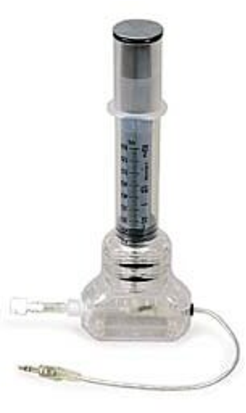
\includegraphics[width=1.5in]{Experiment10Figures/Figure01a.pdf}\hspace{2cm}
    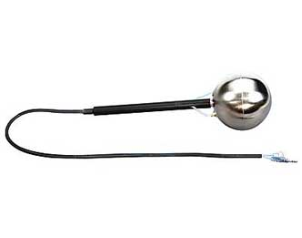
\includegraphics[width=2.0in]{Experiment10Figures/Figure01b.pdf}
  \end{center}
  \caption{The left picture shows the Ideal Gas Law experiment without the PasPort interface. The two cables coming from the syringe are the temperature and pressure connectors. The plunger of the syringe has a mechanical stop to prevent full compression of the syringe.
    The right-hand picture shows the Absolute Zero experiment, again without the PasPort interface. The pressure and temperature connectors are shown exiting at the end of the black cable of the device.}
  \label{H01Fig01}  % the \label command comes AFTER the caption
\end{figure}

\begin{figure}
  \begin{center}
    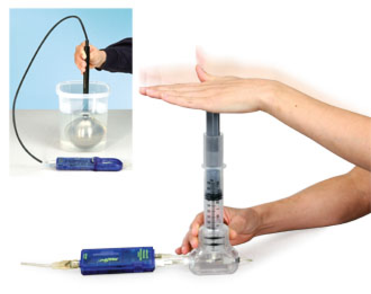
\includegraphics[width=4.0in]{Experiment10Figures/Figure02.pdf}
  \end{center}
  \caption{This picture shows the experimental methods for the Ideal Gas Law (main picture) and Absolute Zero (inlet) experiments. In both cases the temperature and pressure connectors are plugged into the PasPort interface (the small blue box).}
  \label{H01Fig02}
\end{figure}

% Ideal Gas Law
\subsection{The Ideal Gas Law Experiment}

\begin{itemize}
\item[$\triangleright$] Create a Part~1 Data Table for your ideal gas law measurements and calculations. 
\item[$\triangleright$] Open graphs of absolute pressure ($y$-axis) vs. time ($x$-axis) and temperature in Kelvin ($y$-axis) vs. time ($x$-axis) in the \textbf{Capstone} program. Also have a table displaying absolute pressure and temperature open. All these can be opened by double-clicking on the corresponding items on the right-had side of the \textbf{Capstone} program.
\item[$\triangleright$] Disconnect the quick-release pressure connector and push the plunger all the way down. Note that the mechanical stop will prevent the plunger from being pushed all the way to the bottom of the syringe. Record the volume reading on the syringe as the volume $V_{2}$ in your Part~1 Data Table. The value for $V_{2}$ should be about 20 cc.
\item[$\triangleright$] Set the plunger for an initial volume of $V_{1} = 40\,\centi\meter\cubed$.
\item[$\triangleright$] After you have adjusted the volume, re-connect the pressure port.
\item[$\triangleright$] Hold the base of the syringe firmly against a sturdy, flat surface (the lab table).
\item[$\triangleright$] Press the \textbf{Record} button on \textbf{Capstone}.
\item[$\triangleright$] Press straight down as hard as you can on the plunger with the palm of your hand to fully compress the gas inside the syringe. Keep pressing to hold the pressure steady. Important: Do not let the pressure drop for at least 30 s. The mechanical stop will prevent you from decreasing the volume of the gas to less than than about 20 cc. Hold this position until the temperature and pressure have stabilized and are no longer changing (use the data table as an indicator). It should take less than 30 seconds for the temperature to return to room temperature.
\item[$\triangleright$] Release the plunger and allow it to expand back out on its own (it may not go back to 40 \centi\meter\cubed). Wait again until the temperature and pressure have equalized and are no longer changing.
\item[$\triangleright$] Press the \textbf{Record} button again on \textbf{Capstone} to stop recording data.
\end{itemize}


% Analysis with Constant Temperature
\subsubsection{Analysis with Constant Temperature}
\begin{itemize}
\item[$\triangleright$] Highlight an area (click and drag with the mouse) on the pressure graph at the beginning of the data-collecting run, before you compressed the air in the syringe. The highlighted values of the selected data points will appear in the data table of \textbf{Captone}. Record the initial pressure as $P_{1}$ in your Part~1 Data Table.
\item[$\triangleright$] Highlight an area on the pressure graph at the point just before you released the plunger. Record the final pressure as $P_{2}$ in your Part~1 Data Table.
\item[$\triangleright$] Calculate the ratio of initial volume over the final volume, $X_{1} = \nicefrac{V_{1}}{V_{2}}$ and record the result in your Part~1 Data Table.
\item[$\triangleright$] Calculate the ratio of final pressure over the initial pressure, $X_{2} = \nicefrac{P_{2}}{P_{1}}$ and record the result in your Part~1 Data Table.
\item[$\triangleright$] Compare the two ratios. According to the ideal gas law (Eqn.~\ref{eq:idealgas}) the two values should be equal, since $P_{1} V_{1} = P_{2} V_{2}$ for constant temperature (note that the temperature is room temperature in both cases). Discuss, first amongst yourselves and then with your instructor, why the values are different.
\end{itemize}

% Analysis with Varying Temperature
\subsubsection{Analysis with Varying Temperature}

By now you have (hopefully) figured out that you have not accounted for the small amount of volume of air inside the tubing of the apparatus. Using the ideal gas law (Eqn.~\ref{eq:idealgas}) and the data you collected in part 1 you can actually calculate this volume $V_{0}$ by solving the following equation for $V_{0}$
\begin{equation}
  \frac{(V_{1} + V_{0})}{(V_{2} + V_{0})} = \frac{P_{2}}{P_{1}}.
\end{equation}

Using the data from your Part~1 Data Table calculate the value for $V_{0}$ and note the result in your Part~2 Data Table.
\begin{itemize}
\item[$\triangleright$] Highlight an area (click and drag with the mouse) on the temperature graph at the beginning of the data-collecting run, before you compressed the air in the syringe. The highlighted values of the selected data points will appear in the data table of \textbf{Capstone}. Record the initial pressure and the initial temperature as $P_{1}$ and $T_{1}$ in your Part~2 Data Table.
\item[$\triangleright$] Note the initial volume $V_{1}^\prime = V_{1} + V_{0}$ in  your Part~2 Data Table.
\item[$\triangleright$] Highlight the area (click and drag with the mouse) on the temperature graph where the temperature peaks. The highlighted values of the selected data points will appear in the data table of \textbf{Capstone}. Note the peak temperature and the corresponding pressure at this instant as $P_{2}$ and $T_{2}$ in  your Part~2 Data Table.
\item[$\triangleright$] Note the volume $V_{2}^\prime = V_{2} + V_{0}$ in your Part~2 Data Table.
\item[$\triangleright$] Calculate the ratio $Y_{1} = \nicefrac{P_{1} V_{1}^\prime}{T_{1}}$ and record the result in your Part~2 Data Table.
\item[$\triangleright$] Calculate the ratio $Y_{2} = \nicefrac{P_{2} V_{2}^\prime}{T_{2}}$ and record the result in your Part~2 Data Table.
\item[$\triangleright$] Assuming the most significant error is in the volume, compare the difference between the two ratios with your estimate of the uncertainty in the volume.
\end{itemize}

% Measurement of Absolute Zero
\subsection{Measurement of Absolute Zero}

\begin{itemize}
\item[$\triangleright$] Connect the Absolute Zero apparatus to the PasPort system (both the temperature sensor and the quick-release pressure port need to be connected).
\item[$\triangleright$] Close the \textbf{Capstone} Program and re-open it from the desktop.
\item[$\triangleright$] Open a {\bf Table \& Graph} from the main canvas of \textbf{Capstone}. For the $x$-axis of the graph select absolute pressure and for the $y$-axis select temperature in \celsius. For the data table select the same two variables.
\item[$\triangleright$] Now click on the \textbf{Continuous Mode} and select \textbf{Keep mode} from the pull-down menu that will appear. Click on the \textbf{Preview} button to start collecting data.
\item[$\triangleright$] Run the hot water until steam rises from the sink. Fill a pitcher to the 2 quart mark. 
\item[$\triangleright$] First fully submerge the sphere in hot water: Observe the data points appearing on the graph. Make sure the sphere stays completely submerged the entire time you take data. Once the temperature has reached equilibrium (i.e.\ the value in the digital display no longer changes), press the \textbf{Keep Sample} button (N.B.\ Do \textbf{NOT} stop the data collection by clicking on the red square button again). Read and note the values for pressure and temperature (from the digital display) in  your Part~3 Data Table.
\item[$\triangleright$] Next remove half of the water in your container and replace it with cold water from the sink. Again fully submerge the sphere in the water and make sure the sphere stays completely submerged the entire time you take data. Note how the point moves in the Temperature vs. Pressure graph as the values change. Discuss the outcome among yourselves and with your instructor. Once the temperature is stable again (this will take a few minutes) press the \textbf{Keep Sample} button again. Read off and note the values for pressure and temperature (from the digital display) in your Part~3 Data Table.
\item[$\triangleright$] Lastl submerge the sphere in the cold water. Once again you need to make sure the sphere is completely submerged during the time you take data. Note how the point moves in the Temperature vs. Pressure graph as the values change. Discuss the outcome among yourselves and with your instructor. Once the temperature is stable again (this will take a few minutes) press the \textbf{Keep Sample} button again. Read off and note the values for pressure and temperature in your Part~3 Data Table.
\item[$\triangleright$] Press the \textbf{Record}  button once again on DataStudio to stop recording data.
\item[$\triangleright$] Using the fitting tool in \textbf{Capstone}, fit a straight line to the 3 data points you have taken.
\item[$\triangleright$] The $y$-intercept of the best-fit line is the value for absolute zero temperature. Discuss among yourselves and with your instructor why this is the case. Note the result as $T_{0}$ in your Part~2 Data Table.
\item[$\triangleright$] Compare your result to the accepted value of $-273.15\,\celsius$.
\end{itemize}

\section{Data Analysis}

\begin{itemize}
\item[$\triangleright$] Create a table for the analysis at constant temperature including the measured values $V_1, P_1, V_2, P_2$ and the calculated values  $X_1, X_2$.
\item[$\triangleright$] Create a table for the analysis with varying temperature including $V_0, V_1, P_1, V_2, P_2$ and the calculated values  $V^\prime_1, V^\prime_2, Y_1, Y_2$.
\item[$\triangleright$] Create a table for the measurement of absolute zero including the pressure and temperature you measured at the hot, warm and cool temperatures as well as the $y$-intercept and the accepted value of $-273.15\,\celsius$.
\end{itemize}


See Interpretation of Results on next page $===>$

\pagebreak

\section{Post-Lab Submission --- Interpretation of Results}
\begin{itemize}
    \item Make sure to submit your finalized data table (Excel sheet)
    \item Constant Temperature (Isothermal):
        \begin{itemize}
            \item What properties of a system must be proportional if compression is isothermal?
            \item How do the two ratios, $X_{1}$ and $X_{2}$, compare?
            \item What may cause a discrepancy between the ratios of volumes and pressures?
        \end{itemize}
    \item Varying Temperature (Adiabatic):
        \begin{itemize}
            \item What properties of a system must be proportional if compression is adiabatic?
            \item How do the two ratios, $Y_{1}$ and $Y_{2}$, compare?
            \item What may cause a discrepancy between the ratios of volumes and pressures?
            \item Consider the uncertainty as due to volume, do the ratios agree based on that uncertainty range?
        \end{itemize}
    \item Absolute Zero:
        \begin{itemize}
            \item What does absolute zero represent about a system?
            \item What is your extrapolated result for absolute zero; how does it compare to the accepted value?
            \item What measurement uncertainties exist; how do they affect your determined value for absolute zero?
        \end{itemize}
    \item What are possible systematic errors for today's experiments?
\end{itemize}
\newpage
\text{ }
%%%%%%%%%%%%%%%%%%%%%
%                                             %
%                 Experiment M-3              %
%               g with a pendulum             %
%                                             %
%%%%%%%%%%%%%%%%%%%%%

% Hyperref doesn't like math in chapter titles.
%\iffalse
\labChapter{M}{Fluid Physics with Archimedes’ \& Bernoulli’s Principles}
%\else
%\labChapter{M}{FLUIDS}
%\fi
\label{lab:M08_Fluids}


% Background
\section{Background}

Matter most commonly exists as a solid, liquid, or gas; these states are known as the three common phases of matter. We will investigate liquids in today's experiments. While solids are rigid with specific shapes and definite volumes where molecules are locked in position with their neighbors, liquids and gases are considered to be fluids because they are \textit{not rigid} where the molecules are not locked in place and can therefore flow (i.e. move with respect to each other). 

%If an object is placed in a liquid, the object could displace some of the liquid to either float, sink, or stay somewhere in between. If liquid For ideal fluids (negligible viscosity and incompressible) We can also  were to flow through a given area, 

In today's experiments, we seek to understand why objects float or sink in a liquid (water) using Archimedes Principle regarding fluid statics as well as how liquid flows using Bernoulli's Principle regarding fluid dynamics.


\subsection{Archimedes' Principle}

Archimedes' Principle states: ``When an object is submerged in a fluid, the fluid exerts an upwards buoyant force equal to the weight of the fluid displaced by the object."

%When placed in a fluid, some objects float due to a buoyant force. Where does this buoyant force come from? Does it also act on objects that sink? 

As depth increases, pressure in a fluid increases. Therefore, for an object in a fluid, the upward force on the bottom of that object is greater than the downward force on top of that object (see pressure forces $F_{\text{down}}$ vs $F_{\text{up}}$ in Fig.~\ref{M08_fluids_Fig01} \textit{left}). There is a net upward force, or \textbf{buoyant force}, on any object in any fluid. If the buoyant force is greater than the object’s weight, the object will rise to the surface and float. If the buoyant force is less than the object’s weight, the object will sink (depicted in Fig.~\ref{M08_fluids_Fig01}~\textit{right-a} with $F_\text{Buoyancy} < w_\text{object}$). If the buoyant force equals the object’s weight, the object will remain suspended at that depth. As such, there is always a buoyant force acting on an object regardless of whether it floats, sinks, or remains suspended.

\begin{figure}[ht]
  \begin{center}
    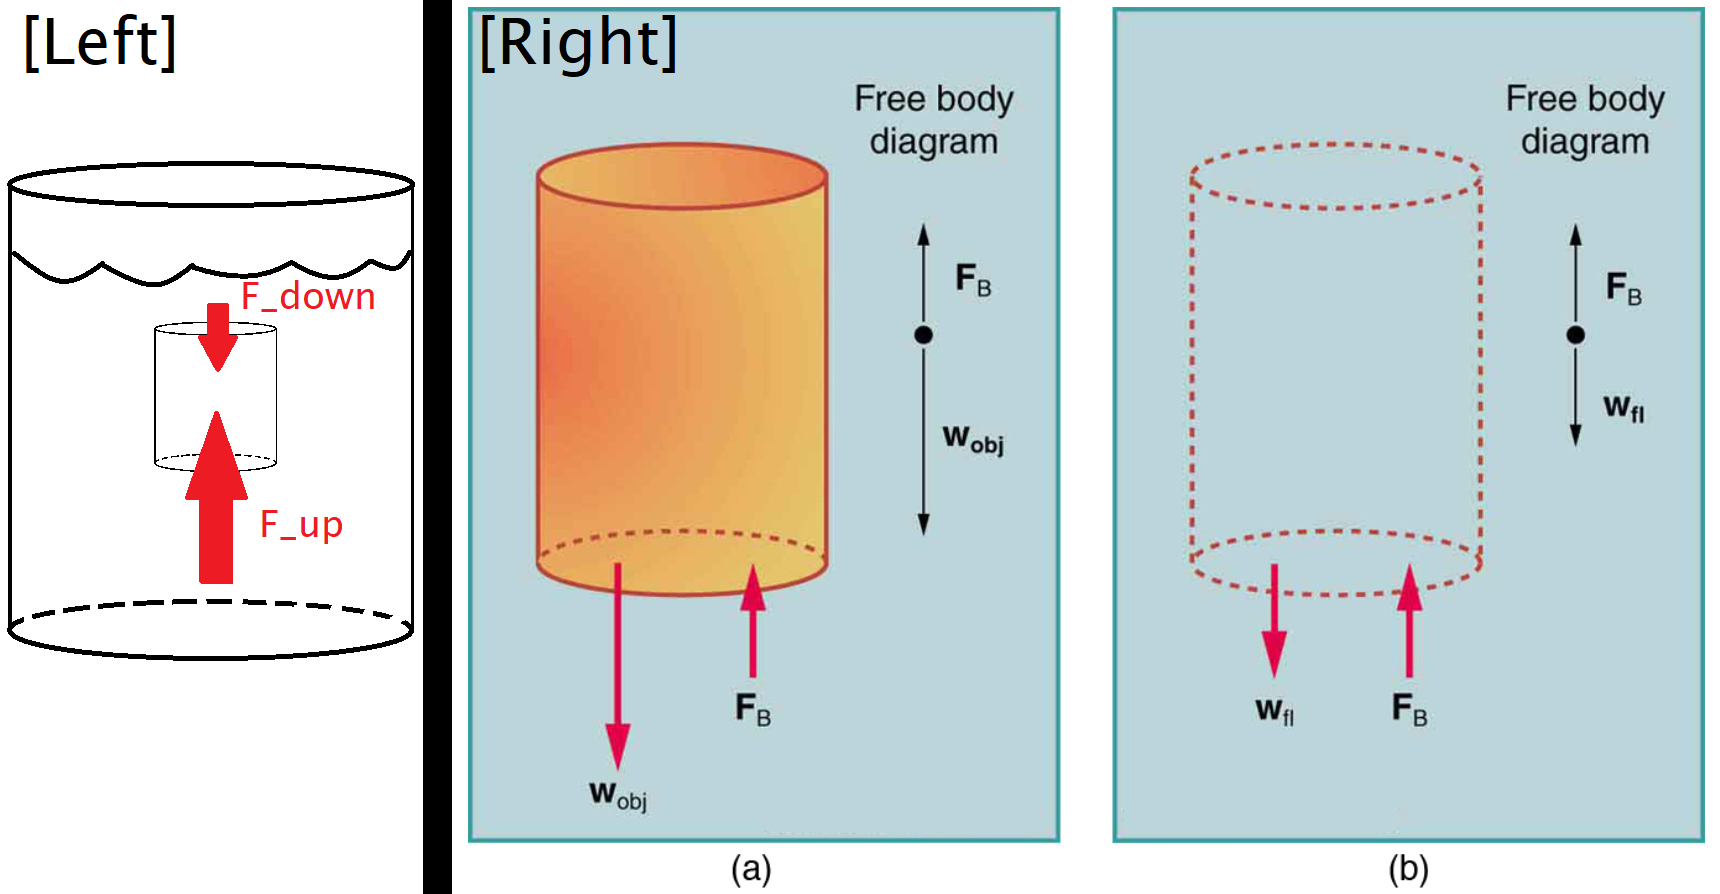
\includegraphics[width=5.3in]{Fall/Experiment08Figures_Fluids/M08_fig00_2.png}
  \end{center}
  \caption{\textbf{\textit{LEFT}}) Pressure due to the weight of a fluid increases with depth causing a greater upward force on the bottom of the object than the smaller downward force on the top of the object. ($F_{\text{down}} < F_{\text{up}}$ and horizontal forces cancel.) \textbf{\textit{RIGHT-a}}) An object submerged in a fluid experiences a buoyant force $F_\text{B}$. If $F_\text{B}$ is greater than the weight of the object $w_\text{obj}$, the object will rise. If $F_\text{B} < w_\text{obj}$ as depicted in \textbf{a}, the object will sink. \textbf{\textit{RIGHT-b}}) If the object is removed, it is replaced by fluid having weight $w_\text{fl}$. Since this weight is supported by surrounding fluid, the buoyant force must equal the weight of the fluid displaced. That is, $F_\text{B} = w_\text{fl}$, a statement of Archimedes’ principle.}
  \label{M08_fluids_Fig01}
  %  \caption{\textbf{\textit{LEFT}}) Pressure due to the weight of a fluid increases with depth since $P=h\rho{}g$. This pressure and associated upward force on the bottom of the cylinder are greater than the downward force on the top of the cylinder. Their difference is the buoyant force $F_\text{B}$. (Horizontal forces cancel.) \textbf{\textit{RIGHT-a}}) An object submerged in a fluid experiences a buoyant force $F_\text{B}$. If $F_\text{B}$ is greater than the weight of the object $w_\text{obj}$, the object will rise. If $F_\text{B} < w_\text{obj}$ as depicted in \textbf{a}, the object will sink. \textbf{\textit{RIGHT-b}}) If the object is removed, it is replaced by fluid having weight $w_\text{fl}$. Since this weight is supported by surrounding fluid, the buoyant force must equal the weight of the fluid displaced. That is, $F_\text{B} = w_\text{fl}$, a statement of Archimedes’ principle.}
\end{figure}

How could we determine the buoyancy force $F_\text{B}$ acting on the object within the fluid? It helps to describe this by removing the object (as in Fig.~\ref{M08_fluids_Fig01}~\textit{right-b}). The volume of the space left behind is filled in by fluid having a weight $w_\text{fl}$. Since that fluid is supported by the surrounding fluid, that weight of the fluid $w_\text{fl}$ (originally displaced by the object) is equal to the buoyancy force $F_\text{B}$. This is \textbf{Archimedes' Principle} --- The buoyant force on an object equals the weight of the fluid it displaces:

\begin{equation}
\label{M08_fluids_Eq01}
    F_\text{B} = w_\text{fl}
\end{equation}


\underline{\textbf{First experiment (Archimedes)}}

In this experiment, we will first determine the mass, volume, and density of 6 objects (see Fig.~\ref{M08_fluids_Fig02}). We will then determine the buoyant force acting on each object using Archimedes' Principle by determining the weight of water each object displaces. Finally, we will determine the buoyant force by measuring the apparent weight of an object.

\begin{figure}[ht]
  \begin{center}
    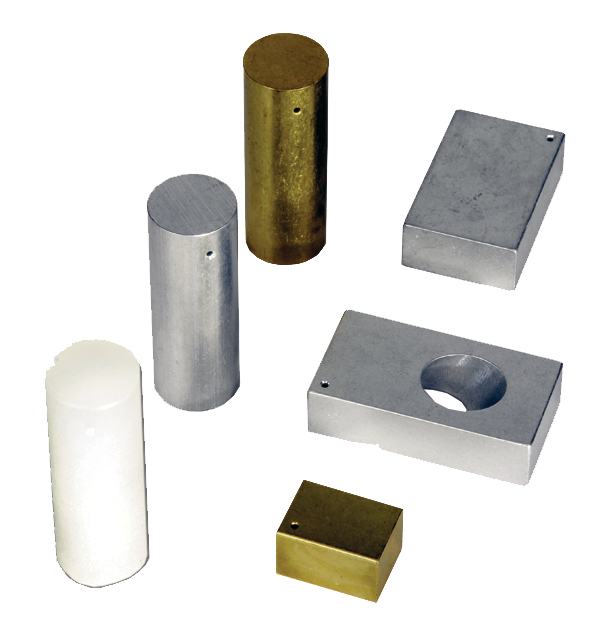
\includegraphics[width=2.9in]{Fall/Experiment08Figures_Fluids/M08_fig02.png}
  \end{center}
%  \caption{3 cylinders (aluminum, brass, plastic), 2 blocks (aluminum, brass), 1 irregular (aluminum).}
  \caption{3 cylinders, 2 blocks, 1 irregular.}
  \label{M08_fluids_Fig02}
\end{figure}

%\underline{\textbf{First experiment, Part I: Mass, Volume, Density}}

As a reminder, the density $\rho$ of an object depends on its mass $m$ and volume $V$:

\begin{equation}
\label{M08_fluids_Eq02}
    \rho = \frac{m}{V}
\end{equation}

and the weight of an object is the downward force due to gravity:

\begin{equation}
\label{M08_fluids_Eq03}
    w_\text{obj} = mg
\end{equation}




\begin{figure}[ht]
  \begin{center}
    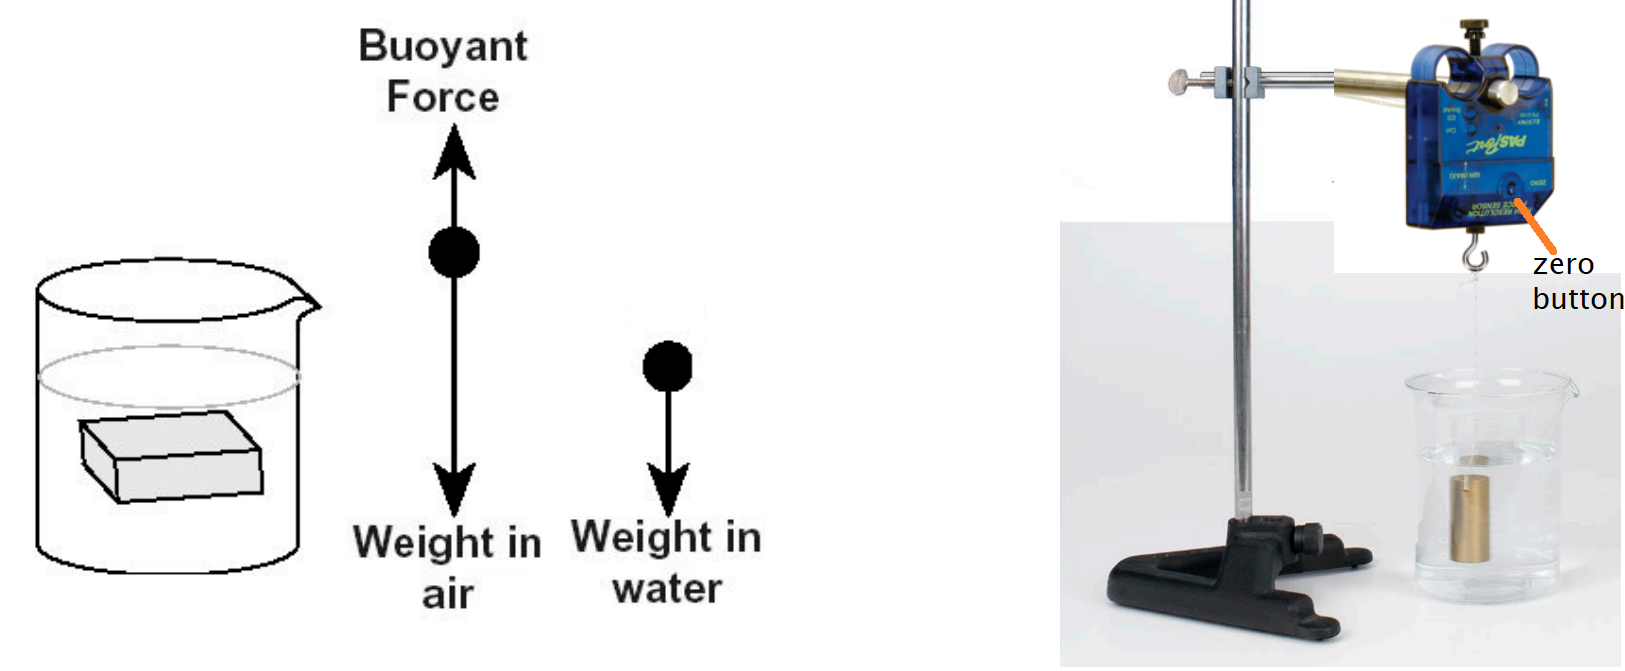
\includegraphics[width=4.9in]{Fall/Experiment08Figures_Fluids/M08_fig06.png}
  \end{center}
%  \caption{3 cylinders (aluminum, brass, plastic), 2 blocks (aluminum, brass), 1 irregular (aluminum).}
  \caption{Left) Force diagram. Apparent weight in water is the difference of weight in air and buoyant force. Right) Force sensor measuring apparent weight of object in water.}
  \label{M08_fluids_Fig04}
\end{figure}

When an object is submerged in a fluid, the apparent weight of the object is less than the weight in air because of the upward buoyant force (see Fig.~\ref{M08_fluids_Fig04}). Thus, the buoyant force can be calculated by finding the difference between the weight of the object in air and the apparent weight of the object when it is submerged in water.

\begin{equation}
\label{M08_fluids_Eq04}
    F_\text{B} = w_\text{obj in air} - w_\text{obj in water}
\end{equation}


%\underline{\textbf{First experiment, Part II: Buoyant Force Using Archimedes' Principle}}
%The buoyant force on several objects is measured by weighing the water displaced by the object as it is submerged. 

%\underline{\textbf{First experiment, Part III: Buoyant Force by Finding the Upward Force}}
%The buoyant force is also determined by measuring the difference between the object's weight in air and its apparent weight in water. Some of the objects have the same density, some have the same volume, and some have the same mass. The density of each object is measured and the dependence of the buoyant force on density, mass, and volume is explored. 

%force sensor rather than lifting the triple beam balance




\subsection{Bernoulli's Principle}

Imagine fluid flowing through a channel of varying width (ex. of such a setup in Fig.~\ref{M08_fluids_Fig07}. As the cross-sectional area changes, the volumetric flow rate remains constant, but the velocity and pressure of the fluid vary.

\begin{figure}[ht]
  \begin{center}
    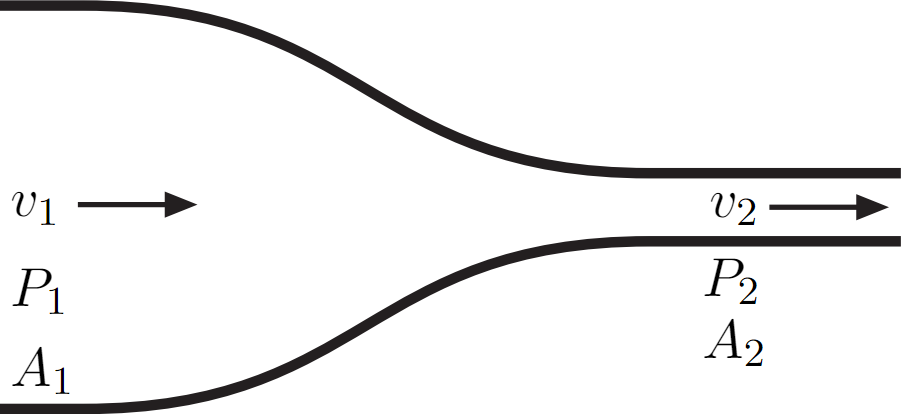
\includegraphics[width=3.9in]{Fall/Experiment08Figures_Fluids/M08_fig07.png}
  \end{center}
  \caption{Example of a Venturi tube, where velocity $v_1 < v_2$, pressure $P_1 > P_2$, and cross-sectional area $A_1 > A_2$}  \label{M08_fluids_Fig07}
\end{figure}

An incompressible fluid of density $\rho$ flows through a pipe of varying diameter. As the cross-sectional area decreases
from $A_1$ (large) to $A_2$ (small), the speed of the fluid increases from $v_1$ to $v_2$. The flow rate, $R = \text{volume}/\text{time}$, of the fluid through the tube is related to the speed of the fluid ($v = \text{distance}/\text{time}$) and the cross-sectional area of the pipe $A$. The flow rate must be constant over the length of the pipe as everything that goes in one side comes out the other end. This relationship is known as the \textbf{Continuity Equation} which can be expressed as:

\begin{equation}
\label{M08_fluids_Eq05}
    R = A_1 v_1 = A_2 v_2
\end{equation}

As the fluid travels from the wide part of the pipe to the constriction, the speed increases from $v_1$ to $v_2$, and the pressure decreases from $P_1$ to $P_2$. This drop in fluid pressure due to fluid speeding up as it flows through a constricted section of a pipe is known as the \textbf{Venturi effect}. This effect can be created with the use of a Venturi tube which allows an incompressible fluid to flow from a wider to narrower section with minimal turbulence.

Assuming the path an incompressible fluid takes is frictionless with no viscous forces, then the energy of the fluid is conserved. The fluid can be analyzed by the total work done on the fluid from the initial position to final position within the tube (total change in both kinetic and potential energy). The full derivation is in your lecture textbook, but for now, we arrive at \textbf{Bernoulli's Equation}. For an \textbf{incompressible, frictionless fluid}, the combination of pressure and the sum of kinetic and potential energy densities is \textit{constant} not only over time, but also along a streamline:

\begin{equation}
\label{M08_fluids_Eq06}
    P + \frac{1}{2}\rho v^2 + \rho g y = \text{constant}
\end{equation}

Note the similarities in Eqn.~\ref{M08_fluids_Eq06} to our previous labs' equations for kinetic and potential energies ($\frac{1}{2}m v^2$ \& $m g h$). Applying this to our Venturi tube of Fig.~\ref{M08_fluids_Fig07}:

\begin{equation}
\label{M08_fluids_Eq07}
    P_1 + \frac{1}{2}\rho v_{1}^2 + \rho g y_1 = P_2 + \frac{1}{2}\rho v_{2}^2 + \rho g y_2
\end{equation}

However, since our tube will be horizontal, we can remove the height dependence and our pressure change is due only to the velocity change (noted by the Continuity Equation in Eqn.~\ref{M08_fluids_Eq05}). Thus, our equation simplifies to \textbf{Bernoulli's Principle} of fluid flow at a \textbf{constant height}:

\begin{equation}
\label{M08_fluids_Eq08}
    P_1 + \frac{1}{2}\rho v_{1}^2 = P_2 + \frac{1}{2}\rho v_{2}^2
\end{equation}


Rearranged another way to determine the pressure at the constriction:

\begin{equation}
\label{M08_fluids_Eq08}
    P_2 = P_1 - \frac{1}{2}\rho (v_{2}^2 - v_{1}^2)
\end{equation}


\underline{\textbf{Second experiment (Bernoulli)}}

In our experiment, we will assume we don't know the pressure at the constriction $P_2$, and will use the Continuity and Bernoulli equations to determine theoretically what $P_2\text{ theoretical}$ should be and compare to the actual value $P_2\text{ actual}$ as measure by our pressure sensor.

The setup will be as in Fig.~\ref{M08_fluids_Fig08}. Water can be released from the pitcher sitting on the white/plexiglass box with the cooler-style spout as the release valve. On the other end of the water hose will be a hose clamp for use during the determination of the flow-rate to rapidly stop the flow of water (if you only used the spout at the pitcher, much of the water would continue flowing out of the tube even after shutting if off, messing up the flow-rate calculations). 

$P_1$, as measured by the Quad Pressure Sensor, will be treated as a known actual or accepted value to be used in our calculations to solve for $P_{2\text{ theoretical}}$. It will be connected to port 1 (or port 3 if in the future these sensors break). 

We will calculate $P_{2\text{ theoretical}}$ from our Continuity and Bernoulli equations. The value of $P_{2\text{, actual}}$, as measured by the Quad Pressure Sensor, will be treated as the known actual value to compare to. $P_2$ will be connected to port 2 (or port 4 if sensor is damaged). 

NOTE: The pressure sensor hoses are to have only (or mostly) air such that water does not reach the pressure sensor. To avoid water getting up the air hoses, ensure the Venturi tube is positioned with the air hoses pointed upward. After passing through the Venturi tube, the water will flow into a catch basin. There will also be a stopwatch to measure flow-rate during the first part of the experiment.

If you require more water in your pitcher, use another pitcher to refill (assuming the catch basin is glass, there will be less of a chance of that breaking if we're not moving it around more than we have to).




\begin{figure}[ht]
  \begin{center}
    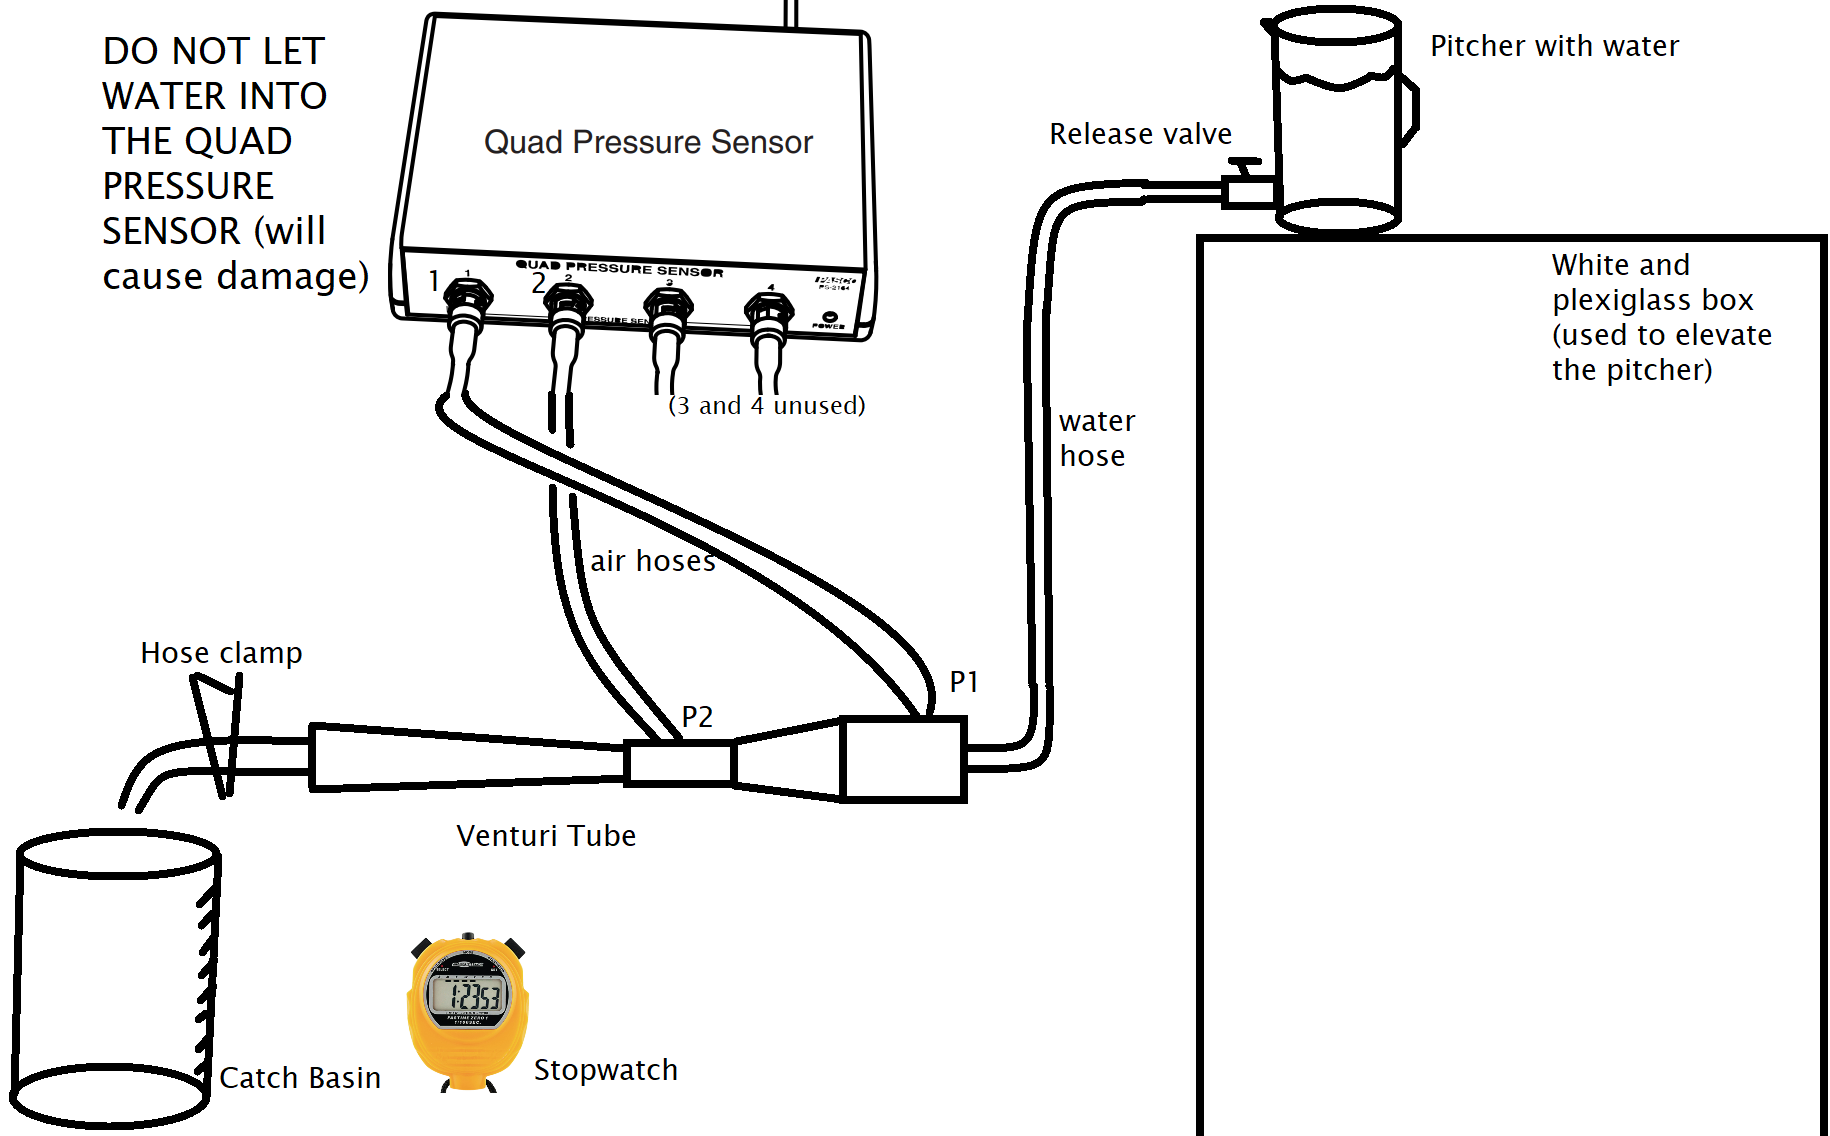
\includegraphics[width=5.9in]{Fall/Experiment08Figures_Fluids/M08_fig08.png}
  \end{center}
  \caption{Sketch of the Venturi tube setup for the second experiment (Bernoulli).}
  \label{M08_fluids_Fig08}
\end{figure}










\section{Experimental Procedure}


\subsection{Archimedes' Principle (First experiment)}

\begin{enumerate}

\item \textbf{OVERALL GOALS:} 
\begin{itemize}
    \item Understand the relationship between buoyancy force and the mass, volume, density of an object.
    %\item Assume \textbf{we know the resistance} of your resistors, but \textbf{we don't know the capacitance} of the capacitors, and we need to determine those C values.
    \item Determine buoyant force using Archimedes' Principle.
    \item Determine buoyant force by measuring the upward force directly.
    %\item Understand  \textit{DISCUSSION POINT}: 
\end{itemize}


\underline{\textbf{Part I: Mass, Volume, and Density}}

\item Create a data table with:
\begin{itemize}
    \item Columns for the mass $m$, relevant dimensions (length, width, height, radius), volume $V$, and density $\rho$
    \item Rows for each of the 6 objects (clearly label or describe the objects in the table).
\end{itemize} 

\item Using the triple-beam balance, find the mass of each of the six objects. List the objects in order from least to greatest mass. \textit{Consider: are any of the masses nearly the same?}

\item Using the calipers, measure the dimensions of the 3 cylinders and the 2 blocks (Fig.~\ref{M08_fluids_Fig03}). Remember to divide the diameter by 2 to get the radius, $r$. Calculate the volume $V$ of these objects %(can use cm$^3$ to be consistent with the irregular shape in the next step). 
$V_\text{cylinder} = \pi r^2 h$ and $V_\text{block} = lwh$

\item There is no simple formula for the volume of the irregularly shaped object, so it is necessary to find the volume by measuring the volume of water it displaces:
\begin{itemize}
    \item Put the beaker under the overflow can spout as shown in Fig.~\ref{M08_fluids_Fig03}.
    \item Pour water into the overflow can until it overflows into the beaker. Allow the water to stop overflowing on its own and empty the beaker into your pitcher and return it to its position under the overflow can spout without jarring the overflow can.
    \item Tie a string on the irregular object.
    \item Gently lower the irregular object into the overflow can until it is completely submerged. Allow the water to stop overflowing and then pour the water from the beaker into the graduated cylinder. Measure the volume of water that was displaced by reading the water level in the graduated cylinder in milliliters (1 ml = 1 cm$^3$)
\end{itemize}

\begin{figure}[ht]
  \begin{center}
    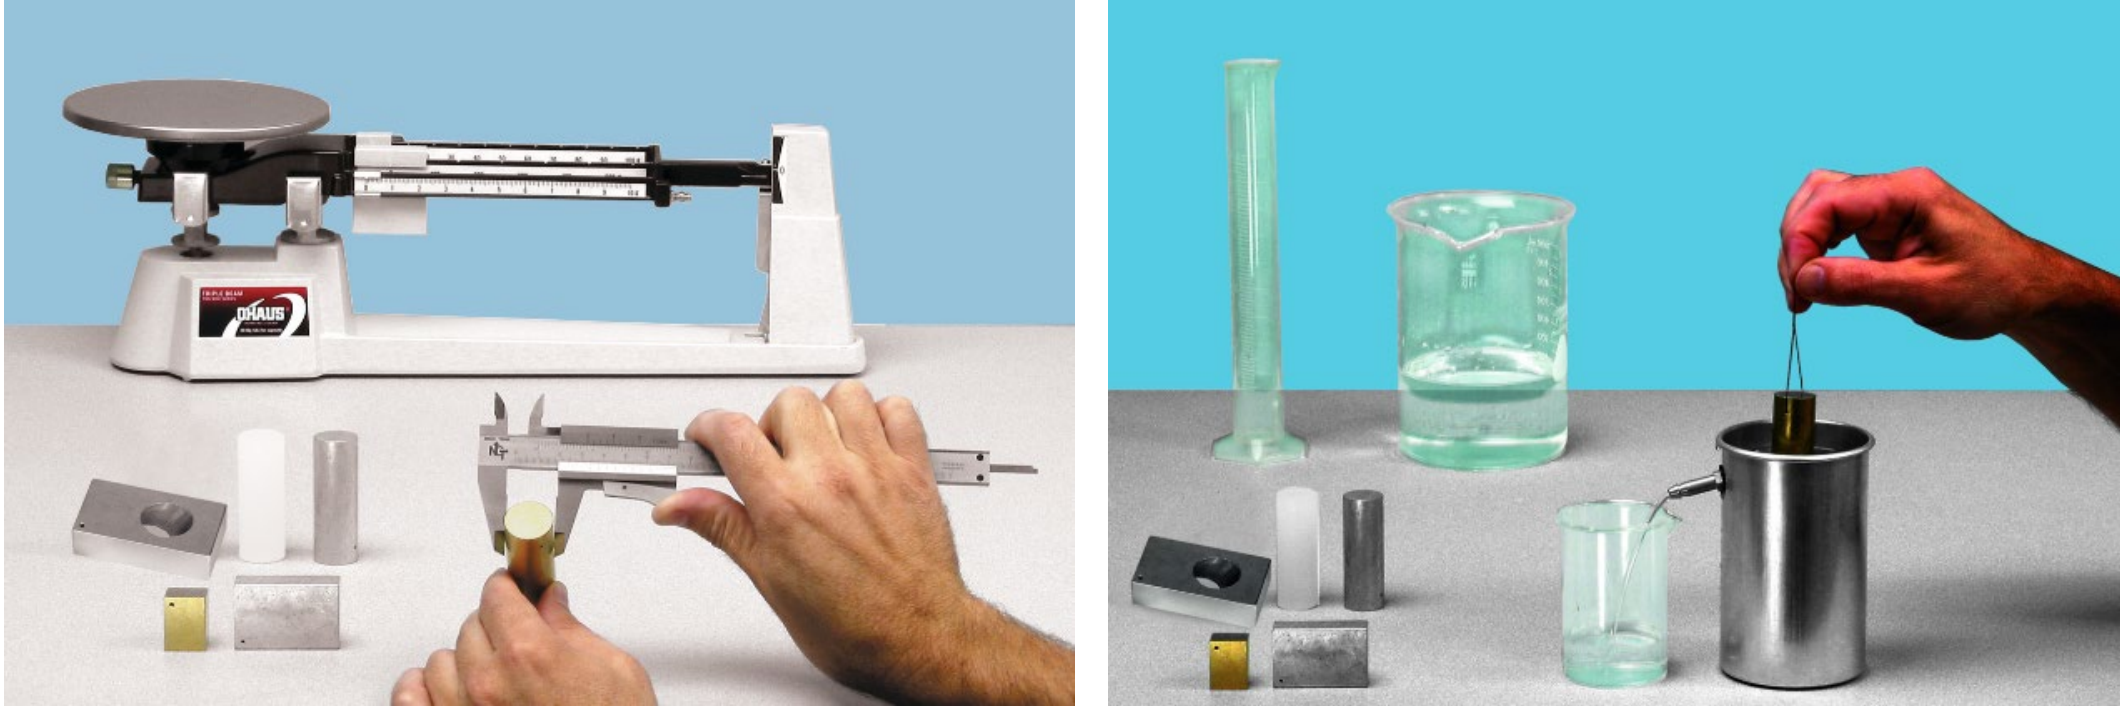
\includegraphics[width=4.9in]{Fall/Experiment08Figures_Fluids/M08_fig03.png}
  \end{center}
  \caption{Left) Measuring with calipers. Right) Lowering object into overflow can.}
  \label{M08_fluids_Fig03}
\end{figure}

\item List the 6 objects in order from least to greatest volume. \textit{Consider: Is this the same order as the mass list? Are any of the volumes nearly the same?}

\item Calculate the density of each object. List the 6 objects in order from least to greatest density. \textit{Consider: Is this list in the same order as either the mass list or the volume list? Do any of the objects have densities that are nearly the same?}

\item Group the objects according to the type of material of which they are made. \textit{Consider: In which list (mass, volume, or density) are the objects grouped similarly?}

%\item Create a data table:



\underline{\textbf{Part II: Finding the Buoyant Force Using Archimedes' Principle}}

For each of the objects, find the weight of the water displaced by each one:

\item Create a data table with:
\begin{itemize}
    \item Mass of beaker and other common data
    \item Columns for the mass $m_\text{water} = m_\text{total} - m_\text{beaker}$, weight $w_\text{water} = m_\text{water} g = F_\text{B}$
    \item Rows for each of the 6 objects plus a half-submerged brass cylinder (so 7 rows). Clearly label or describe the objects in the table.
\end{itemize} 
\item Find the mass of the beaker. Put the beaker under the overflow can spout as shown in Fig.~\ref{M08_fluids_Fig03}.
\item Pour water into the overflow can until it overflows into the beaker. Allow the water to stop overflowing on its own and empty the beaker into the pitcher and return it to its position under the overflow can spout without jarring the overflow can.
\item Tie a string onto each of the objects.
\item Gently lower the first object into the overflow can until it is completely submerged. Allow the water to stop overflowing. Find the mass of the water plus beaker. Subtract the mass of the beaker to determine the mass of the displaced water. Multiply the mass by the acceleration due to gravity (9.803 m/s$^2$) to find the weight of the water.
\item Repeat this procedure for the other objects. Note that the plastic cylinder will float so don’t try to completely submerge it in the water. Also find the weight of the displaced water when only half the brass cylinder is submerged.
\item List the objects in order from least buoyant force to greatest buoyant force. \textit{Consider: Is this in the same order as the mass list, the volume list, or the density list? Are any of the buoyant forces nearly the same? Why or why not?}


\underline{\textbf{Part III: Finding the Buoyant Force by Finding the Upward Force}}

\item Create a data table:
\begin{itemize}
    \item Seven rows for each of the 6 objects as well as the brass cylinder half-submerged (clearly label or describe the objects in the table).
    \item Columns for weight in air $w_\text{obj in air}$, apparent weight in water $w_\text{obj in water}$, buoyant force $F_\text{B}$ as determined with Eqn.~\ref{M08_fluids_Eq04}.
\end{itemize}
\item Tie a loop on the other end of the string so it can be hooked onto the force sensor.
\item In Capstone, press record or monitor, and you will see the force in Newtons displayed (constantly updating). You can let this continue running to act as a continuous scale.
\item Before hanging any of the objects on the force sensor hook, zero the force sensor with the physical ``zero" button on the front of the force sensor (shown in Fig.~\ref{M08_fluids_Fig04}).
\item With the water out of the way, record the weight of each object in air $w_\text{air}$ by hanging them on the hook. 
\item Zero the sensor as needed if it appears to be drifting when swapping out the different objects.
\item Now place the pitcher of water beneath the force sensor such that when you hang each object from the force sensor hook, the objects can be fully submerged. Record the apparent weight of each object in water $w_\text{water}$.
\item Calculate the buoyant force for each object by taking the difference between the weight in air and the weight in water (Eqn.~\ref{M08_fluids_Eq04}).
\item Add an additional column and calculate for each object case the \% difference between the buoyancy force (found here by measuring the upward force) and the buoyancy force found previously by Archimedes' Principle of the displaced water. 

$\% \text{ diff.} = \frac{F_\text{B, upward force method} - F_\text{B, Archimedes' method}}{F_\text{B, Archimedes' method}} \times 100$ 

\textit{Consider: In each case, is the buoyant force that was determined using the upward force equal to the
weight of the water displaced?}



\end{enumerate}





\subsection{Bernoulli's Principle (Second experiment)}

\begin{enumerate}

\item \textbf{OVERALL GOALS:} 
\begin{itemize}
    \item Understand fluid-flow continuity through different constrictions.
    %\item Assume \textbf{we know the resistance} of your resistors, but \textbf{we don't know the capacitance} of the capacitors, and we need to determine those C values.
    \item Determine flow-rate of our system using the Continuity Equation.
    \item Understand Bernoulli's Principle of fluid flow at a constant height to investigate the Venturi effect and determine the pressure of a fluid at a constriction point (in a Venturi tube).
    %\item Understand  \textit{DISCUSSION POINT}: 
\end{itemize}


\underline{\textbf{Part I: Determining Flow Rate $R$}}
\item Create a data table:
\begin{itemize}
    \item 6 rows for five trials of the measuring flow rate as well as the average flow rate $R_\text{avg}$ and standard deviation of your flow rate $\sigma_R$.
    \item Columns for the volume $\Delta V$ of water, elapsed time $\Delta t$ it took to flow, and flow rate $R$.
\end{itemize}
    \item With water in the pitcher, open the release-valve (spout) to allow water to flow and remove most of any air bubbles within the tubing. After a couple seconds, tighten the hose clamp at the end to halt the flow. Take whatever water is in the catch basin and return it to the pitcher.
    \item Start current trial with the catch basin empty.
    \item Start the stopwatch and open the hose clamp at the same time to start water flow.
    \item After a measurable amount of water has flowed through, stop the stopwatch and close the hose clamp at the same time.
    \item Measure the volume of water that flowed out of (or into) the apparatus (either with the scale on the catch basin or graduated cylinder).
    \item Calculate the average flow rate for the current trial $R = \frac{\Delta V}{\Delta t}$ where $\Delta V$ is the volume of water and $\Delta t$ is the elapsed time.
    \item Empty the catch basin or graduated cylinder back into the pitcher to keep a consistent amount of water in it.
    \item Rerun this process starting with the empty catch basin (assuming the water hose is still clear of air bubbles) 4 more times for a total of 5 trials.
    \item From the individual trial flow rates, calculate the average flow rate $R_\text{avg}$ and standard deviation $\sigma_R$ which we will use to represent our uncertainty in the flow rate ($R_\text{avg} \pm \sigma_R$).
    \item NOTE: Typically the flow rate varies with the level of water in the reservoir. To keep the flow rate close to constant, make the pressure measurements with the water level approximately the same as it was for the flow rate measurement.



\underline{\textbf{Part II: Determining Pressure at a Constriction}}

\hspace{6mm}\underline{\textbf{with Continuity and Bernoulli Eqns.}}

\item Create a data table:
\begin{itemize}
    \item Common data section including:
    \begin{itemize}
        \item Flow rate $R_\text{avg} \pm \sigma_R$ from Part I.
        \item Cross-sectional areas $A_1$ and $A_2$ and their uncertainties $\delta_{A_1}$ and $\delta_{A_2}$.
        \item Velocities $v_1$ and $v_2$. Also include the max values for each (Used to estimate pressure uncertainty later).
        \item Density of water $\rho$ (use 1000 kg/m$^3$)
    \end{itemize}

    \item 7 rows for five trials of the measuring $P_1$ and $P_2$ in Capstone as well as their averages $P_{1\text{ avg actual}}$ and $P_{2\text{ avg actual}}$ and standard deviations $\sigma_{P_{1\text{ avg actual}}}$ and $\sigma_{P_{2\text{ avg actual}}}$.
    \item Columns for $P_1$ and $P_2$.
\end{itemize}

    \item Determine the cross-sectional areas of the wide and narrow constrictions ($A_1$ and $A_2$ respectively) with the calipers from the cutaway version of the Venturi tubes ($A = \pi r^2$). Note your uncertainty due to your measurement precision ($\delta_{A_1}$ and $\delta_{A_2}$).
    \item Calculate $v_1$ and $v_2$ with the Continuity Eqn.~\ref{M08_fluids_Eq05} based on your measured areas and average flow rate. Similarly, calculate $v_{1\text{ max}}$ and $v_{2\text{ max}}$ by maximizing the flow rate ($R_\text{avg} + \sigma_R$) and minimizing the areas (e.g. $A_1 - \delta_{A_1}$).

\item Capstone will be set up to show two pressures representing $P_1$ and $P_2$. Double check the the pressure taps of the Venturi tube are appropriately connected like in Fig.~\ref{M08_fluids_Fig08} where Channel 1 is connected to the wider part of the Venturi tube, and Channel 2 to the narrow constriction of the Venturi tube. (It'll be easier to keep track of which pressure is which when the labels are similar.) 
\item Capstone will also show a plot with both $P_1$ and $P_2$ on the y-axis as a function of time on the x-axis. To analyze either data set later on, you can click directly on the plotted data.
\item Calibrate the pressure sensor by:
\begin{itemize}
    \item Ensure both the hose clamp and release valve (spout) are closed.
    \item Disconnect the air hoses from the Quad Pressure Sensor via the quick connectors so the pressure sensors are open to atmospheric pressure. Set the air hoses on top of the white box (or in a bracket to hold them if I get them prepared in time) so the end of the hose is above the spout water level to prevent water from siphoning through the air hoses.
    \item In Capstone, select the green Calibration tab on the left-hand panel.
    \item 1) Pressure 2) Select all ``Pressure Measurements" 3) Type of Calibration as ``One Standard (1 point offset)" 4) Set Standard Value to average atmospheric pressure of 101.3 kPa --- Click the "Set Current Value to Standard Value" button 5) Finish
    \item Both Absolute Pressure Channels 1 and 2, when you press record, should now read at about 101.3 kPa, if not, retry the calibration.
\end{itemize}
\item Ensure no water is near the end of the air hoses to prevent any water getting into the pressure sensors. Reconnect the air hoses to the pressure sensors.
\item You can open the hose clamp at the end of the hose as it will not be needed for the rest of this experiment. You will just need to catch basin to collect the water and avoid making a mess.
\item Press record, then open the release valve to allow the water to flow into the catch basin. After any air bubbles have passed and the water is flowing with minimal turbulence, continue recording pressure data for $\sim$5~seconds, then close the release valve (spout) and stop recording.
\label{M08_fluids_BernoulliStep_00}
\item Find the section of your Pressure vs. Time plot where flow was laminar (smooth without bubbles), should be a generally flat section of the Pressure vs Time plot. Click on the $P_1$ data on the plot, enable the highlight tool, and select a chunk of the plot when flow was laminar (no bubbles, the flat part). Do the same for the $P_2$ data. You can find the average value for $P_1$ and $P_2$ at the bottom of the table on the left hand side of your screen, where the mean is representing the average value of whichever subset of the data you've highlighted.
\item Record both $P_{1\text{ actual}}$ and $P_{2\text{ actual}}$. There should be a difference of $\sim 2 \text{--} 5$kPa, if not, double check with an instructor.
\item Rerun this process from Step~\ref{M08_fluids_BernoulliStep_00} an additional 4 times for a total of 5 trials.
\item Determine the $P_{1\text{ avg actual}}$ and $P_{2\text{ avg actual}}$ values from your five trials. Also determine their standard deviations $\sigma_{P_{1\text{ avg actual}}}$ and $\sigma_{P_{2\text{ avg actual}}}$.
\item Calculate your theoretical value of $P_{2\text{ theoretical}}$ with Eqn.~\ref{M08_fluids_Eq08} using your previously determined velocities $v_1$ and $v_2$ and your average $P_{1\text{ avg actual}}$ treated as the known actual value for the wider part of the Venturi tube.
\item Similarly calculate your max theoretical value of $P_{2\text{, max theoretical}}$ by maximizing ${P_{1\text{ avg actual}}}$ (e.g. ${P_{1\text{ avg actual}}} + \sigma_{P_{1\text{ avg actual}}}$) and using your already determined maximized velocities $v_{1\text{ max}}$ and $v_{2\text{ max}}$.
\item Represent your uncertainty $\delta P_{2\text{ theoretical}}$ with the difference of your maximized value and average values (e.g. $\delta P_{2\text{ theoretical}} = P_{2\text{, max theoretical}} - P_{2\text{ theoretical}}$).
\item \textit{Consider:} Does you theoretical value for $P_2$ agree with the actual value of $P_2$ as measured with the pressure sensor?



















    
\end{enumerate}











%\pagebreak

\section{Post-Lab Submission --- Interpretation of Results}

\subsection{Archimedes' Principle (First experiment)}
\begin{itemize}
\item Make sure to submit your finalized data table (Excel sheet)

    \item First Experiment (Archimedes' Principle)
\begin{itemize}
    \item In which list (mass, volume, or density) are the objects grouped similarly?
    \item In each object case, is the buoyant force that was determined using the upward force (Part III) equal to the
weight of the water displaced (Part II)? Were the \% differences between the two methods for each case relatively small, or did any case standout?
    \item Which objects had the same buoyant force when submerged? Why?
    \item For the plastic cylinder, what was the apparent weight in water? What would be the buoyant force be if plastic cylinder were completely submerged?
    \item How did the buoyant force for the totally submerged brass cylinder relate to the buoyant force for the half-submerged brass cylinder?
    \item What does the buoyant force depend on: The mass of the object, or its volume, or its density, or the material from which it is made?
\end{itemize}


    \item Second Experiment (Bernoulli's Principle)
\begin{itemize}
    \item Does you theoretical value for $P_2$ agree with the actual value of $P_2$ as measured with the pressure sensor? \newline (i.e. $P_{2\text{ theoretical}} \pm \delta P_{2\text{ theoretical}}$ overlap with $P_{2\text{ avg actual}} \pm \sigma P_{2\text{ avg actual}}$?)
    \item How is the Bernoulli Principle different than the Bernoulli Equation?
    \item What assumptions about the fluid allows the Bernoulli Principle to work? (i.e. what type or characteristics of the fluid and/or flow are necessary assumptions for Bernoulli to hold true?)
    \item Imagine that instead of being on the table, the Venturi tube were set on the floor with the rest of the experimental apparatus unchanged. Would the difference in pressures we see on the Capstone plot between $P_1$ and $P_2$ during the smooth, laminar flow section that we analyzed to find average pressures be \textit{larger}, \textit{smaller}, or \textit{the same}. Why?
\end{itemize}


    

\end{itemize}
%%%%%%%%%%%%%%%%%%%%%
%                                              %
%                 Experiment M-9               %
%                Harmonic Motion               %
%                                              %
%%%%%%%%%%%%%%%%%%%%%

%\labChapter{M}{Simple \& Damped Harmonic Motion}
\labChapter{M}{Simple \& Damped Harmonic Motion with Springs \& Glider on Level Air Track}
\label{lab:M9}

% Introduction
%\section{Introduction}
\section{Background}

!!!!!!!!!!!!!!! Re-lable springs as A and B, then use 1 and 2 to represent stretched lengths

When the magnitude of the net force acting on a body is linearly related to the displacement of the body and is acting in a direction opposite to the displacement, the body will oscillate in simple harmonic motion around the point where the net force is zero.  We will investigate the one-dimensional motion of a mass which is constrained by a net force $F = -k x$. This linearly related force is said to be obeying Hooke's Law.  That is to say, if the mass is displaced a distance $x$, a restoring force will act in a direction opposite to the displacement with a magnitude equal to the spring constant, $k$, times the magnitude $x$.  The independence of the period on the amplitude and the effect of energy loss mechanisms on the motion will also be examined.


Consider the system illustrated in Fig.~\ref{M09Fig01}.  The mass is assumed to be resting on a frictionless surface and is constrained by the two springs shown.

\begin{figure}
  \begin{center}
    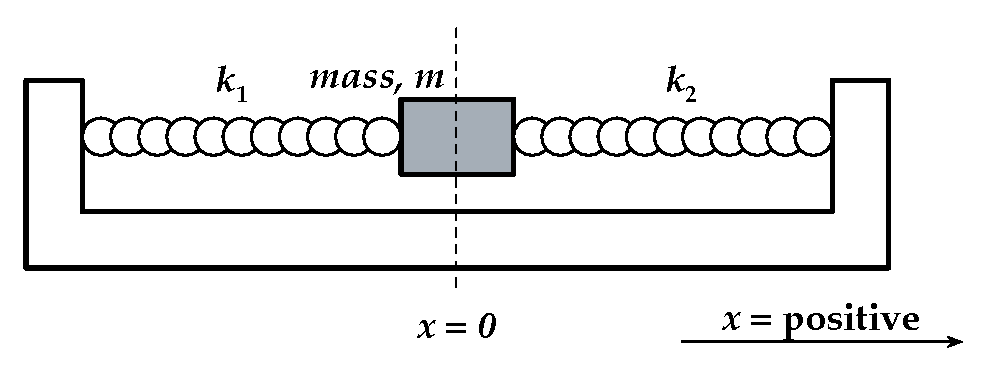
\includegraphics[width=5.5in]{Experiment07Figures/Figure01.pdf}
  \end{center}
  \caption{System sketch for Harmonic Motion experiment.}
  \label{M09Fig01}  % the \label command comes AFTER the caption
\end{figure}

The springs each apply a force according to Hooke's Law as follows
\begin{eqnarray*}
  F_1 & = & -k_1\, x - F_0\\
  F_2 & = & -k_2\, x + F_0.
\end{eqnarray*}
When $x = 0$, each spring pulls an equal and opposite amount $F_0$ resulting in a net force of $F = F_1 + F_2 = 0$ at the center equilibrium position.

When the mass is displaced to some point $x$, the net force $F(x)$ is given by
\[
F(x) = F_1(x) + F_2(x) = -(k_1 + k_2) x.
\]
These two springs acting together in this manner produce a force $F(x) = -k_{eff} x$, where $k_{eff} = k_1 + k_2$, or we can say that the force on the mass acts as if one spring was tied to it with an effective spring constant $k_{eff}$.

If we displace the mass to some position $x = A$ and release it at time $t = 0$, we can determine how the mass will move as a function of time under the influence of the restoring force $F(x)$.  Using Newton's Second Law and the definition of the acceleration $a$, we can write
\begin{equation}
  \label{eq:M09fx}
  F(x) = m\, a = m \frac{{\rm d}^{2}x}{{\rm d} t^{2}} = -k x.
\end{equation}
In order to find a solution to this equation, we need to find a function $x(t)$ whose second derivative is the same as the function itself, give or take a constant or two.  One such function $x(t)$ is
\begin{equation}
  \label{eq:M09xt}
  x(t) = A \cos\left(\omega t \right).
\end{equation}
where $A$ and $\omega$ are constants.  In order to evaluate the constants we observe what the function $x(t)$ must be at known points.  One such point is $t = 0$ where $x = A$, that is the release point of the displaced mass.  If we substitute the function $x(t)$ into Eqn.~\ref{eq:M09fx}, we will find that it satisfies the equation if
\begin{equation}
  \label{eq:M09omega}
  \omega = \sqrt{\frac{k}{m}}.
\end{equation}

The quantity $\omega$ is called the angular frequency.  From Eqn.~\ref{eq:M09xt}, we see that the position of the mass oscillates between the points $+A$ and $-A$ as the cosine function oscillates between $+1$ and $-1$ as a function of time.  The cosine makes one complete oscillation from $+1$ to $-1$ to $+1$ when the quantity $\omega t$ goes through $2\pi$ radians.  The elapsed time for this one complete oscillation is $T$, the period.  Thus $\omega T = 2 \pi$, or
\[
\omega = \frac{2\pi}{T}.
\]

If the period is the time it takes the mass to make one complete cycle, the frequency will be $f = (1/T)$ or $\omega = 2\pi f$.  Using Eqn.~\ref{eq:M09omega} we can write the period as
\begin{equation}
  \label{eq:M09period}
  T = 2 \pi \sqrt{\frac{m}{k}}.
\end{equation}
Note that the period of oscillation is independent of the amplitude $A$ of the oscillation for this case where there are no energy loss mechanisms.

When the system is started, the mass was displaced a distance $A$ and then released.  When the system is displaced that distance $A$, a certain energy is given to the system in the form of potential energy stored in the springs in the amount of $U=(1/2) k A^{2}$.  Thereafter, this initial energy is the total mechanical energy of the system, and without any energy loss mechanisms, the total energy remains constant.  Thus, as the mass moves, it exchanges potential and kinetic energy.  If no energy is lost, the mass will always oscillate between the same amplitude $+A$ and $-A$.  It will also have the same maximum kinetic energy which occurs at the $x = 0$, or equilibrium position.  You can see from Eqn.~\ref{eq:M09xt} and its derivatives, that the displacement, velocity, and acceleration of the mass are related as:
\begin{eqnarray*}
  x(t) &=&  A          \cos(\omega t),\\
  v(t) &=& -A \omega   \sin(\omega t),\\
  a(t) &=& -A \omega^2 \cos(\omega t).
\end{eqnarray*}
The maximum values of $v(t)$ and $a(t)$ are dependent on the amplitude $A$.  Assume now that there is some energy loss mechanism present as the mass oscillates, e.g.\ some friction on the surface on which the mass is sliding or some air drag on the mass.  If energy is lost to such a nonconservative force, then the total energy of the system will decrease.  As the total energy decreases, the amplitude, along with the maximum velocity and acceleration will also decrease.  Since neither the period nor the frequency of oscillation are functions of the amplitude, they should remain constant.  This kind of motion is called damped harmonic motion.

The opposite effect is also true.  If a little bit of energy is added during each cycle, then the total energy of the system will increase and be manifested by an increase in amplitude and still no change in period.

In the laboratory, we will measure the spring constants of two almost identical springs by applying a known force and measuring the stretching (the displacement) of each of the springs.  These two springs will then be configured with a mass on a frictionless surface (a glider on an airtrack) as illustrated in Fig.~\ref{M09Fig01}.  We will set the mass in motion by releasing it from a displacement point and measuring the period of oscillation.  This measured period will be compared with the calculated value obtained from Eqn.~\ref{eq:M09period}.

The independence of the period on amplitude will be examined by measuring the period for the mass started with various amplitudes.  We will also observe the behavior of the motion of the oscillating mass in a case where the energy loss mechanism will be dramatically increased by placing a sail on the glider to increase the air drag.


\pagebreak

\section{Experimental Procedure}

Before assembling the glider and springs on the airtrack, we will determine the spring constants of the two springs.  These very light springs are capable of stretching 20 times their rest length.  Please be very careful not to damage them through careless handling or overstretching.

\begin{figure}
  \centering
  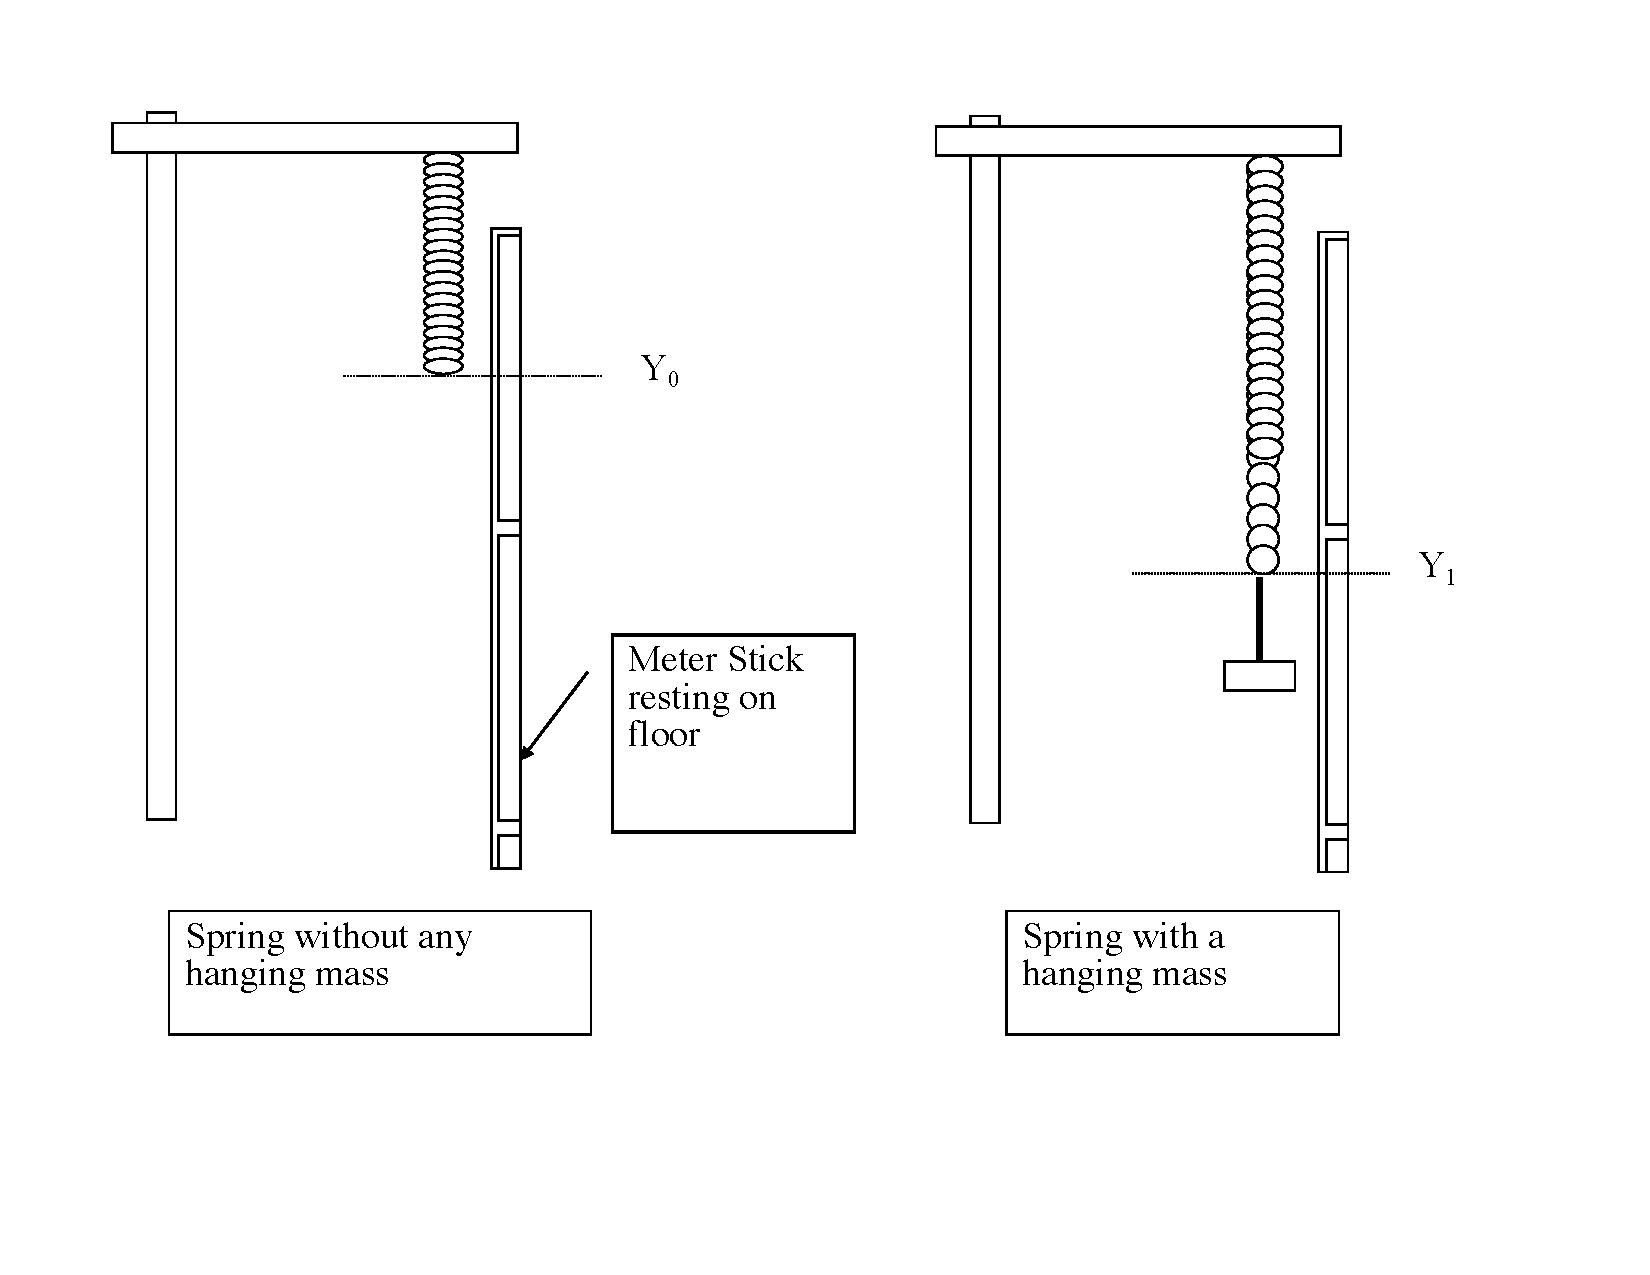
\includegraphics[width=6.0in]{Experiment07Figures/Figure02.pdf}
  \caption{Experimental Method to measure $\Delta y$ for a spring in Experiment M-\ref{lab:M9}}
  \label{M09Fig02}
\end{figure}

\begin{itemize}
\item For each spring perform the following steps to determine its average spring constant $k_{\text{spring }n}$.  Refer to Fig.~\ref{M09Fig02}.
  \begin{enumerate}
  \item Orient the 2-meter stick with the zero end at the top. It is only the change in $y$ with force that matters in this measurement. 
  \item Attach one end of the spring to the ring stand and allow the spring to hang free with no mass hanging. Record $y_0$.
  %\item Carefully hang a 50~\gram\ weight holder on the end of the spring and record $y_1$. Take the measurements with the spring and any weights hanging stationary.
  \item Carefully hang enough mass on a weight holder on the end of the spring until it extends a total displacement of $\sim 0.95 \meter$ from $y_0$ and record the exact distance $y_1$ and mass used as $m_1$ (don't forget the hanger is 50 grams itself). Take the measurements with the spring and any weights hanging stationary.
    %  \item Displace the 50~\gram\ weight holder 2.0~\centi\metre\ release it. Measure the time for 20 oscillations and divide by 20 to obtain the period of the spring with the hanging 50 gram weight holder.
  %\item Add an additional 20~\gram\ to the weight holder and repeat steps 1--3.
  \item Add a additional mass to the weight holder on the end of the spring until it extends a total displacement of $\sim 1.55 \meter$ from $y_0$ and record the exact distance $y_2$ and mass used as $m_2$ (don't forget the hanger is 50 grams itself). Take the measurements with the spring and any weights hanging stationary.
    \item Calculate and record the two values of $k$ for the current spring.  The first is $k_{1\text{,spring1}}=m_1 \,g/(y_1 - y_0)$.  The second is $k_{2\text{,spring1}}=m_2 \,g/(y_2 - y_0)$.
    \item Repeat the above steps for the second spring to find $k_{1\text{,spring2}}$ and $k_{2\text{,spring2}}$.
    %  \item Average the values of $k$ for the spring and record $k$ for that spring and the standard deviation. See Eqn.~\ref{eq:errorSigmaX}.
    %  \item Average the period for that spring and calculate the standard deviation.
  \end{enumerate}
  \item Calculate the average values for $k_{\text{spring1}}$ and $k_{\text{spring2}}$ and then determine the effective spring constant $k_{eff} = k_{\text{spring1}} + k_{\text{spring2}}$ that will be acting on the glider.
\item Turn on the air supply to the airtrack and allow it to flow for several minutes.
\item Measure the mass of the larger glider and place it on the track.
\item \textbf{CASE 1:} Use the scale on the track and a corner of a glider to determine various displacements along the track.
  \begin{enumerate}
  \item Assemble the larger glider on the track and attach the springs to the glider and the ends of the track as in Fig.~\ref{M09Fig01}.  Again please be careful not to overstretch the springs or allow them to snap back.
  \item To determine the period of oscillation of the mass, displace the mass 10~\centi\metre\ from its equilibrium position and release it. When the mass returns to its starting point, start the stopwatch at the zero velocity point.  Allow the mass to oscillate through 10 complete cycles and stop the stopwatch at the zero velocity point at the end of the tenth cycle. That will be essentially the starting point.  Record the time for the ten cycles and divide by 10 to obtain the period.
  \item Using the same cart, find the period for starting amplitudes of 15, 20, 25, and 30~\centi\metre.
  \item Calculate the expected period from Eqn.~\ref{eq:M09period} and compare it with each of the measured values for the different starting amplitudes.
  \end{enumerate} 
\item \textbf{CASE 2 \& 3:} Measure the mass of the small glider with and without the sail-holder and sail. Reassemble the system with the smaller glider without the sail assembly on the track.
  \begin{enumerate}
  \item Using the same measuring technique as used with the larger glider, determine the period for a starting amplitude of 10~\centi\metre.  Record the time for ten cycles and divide by 10 to obtain the period.
  \item Using the same cart, find the period for starting amplitudes of 15, 20, 25, and 30~\centi\metre.
  \item Calculate the expected period from Eqn.~\ref{eq:M09period} and compare it with each of the measured values for the different starting amplitudes.
  \item Place the paper sail assembly on the glider.
  \item Use a starting amplitude of 25~\centi\metre\ from the equilibrium position.  Record both the equilibrium position and your starting point; determine and record the amplitude (should be 25 cm).  Each of the following steps will be started from this same amplitude point.
    %\item Pick a convenient amplitude point approximately 25~\centi\metre\ (but NOT greater than 30~\centi\metre!) from the equilibrium position.  Record both the equilibrium position and your starting point; determine and record the amplitude.  Each of the following steps will be started from this same amplitude point.
    \begin{enumerate}%[label=(\Alph*)]
    \item Displace the glider with its sail to the starting point and release it.  At the end of the fifth cycle, capture the glider by gently pressing your finger on the edge of the glider as gets to its maximum amplitude point, i.e.\ $v = 0$.  Record the amplitude.  Be sure to use the same point on the glider that you used to determine the equilibrium point and the 25~\centi\metre\ starting point.  Measure the total time for the cycles and divide by the number of cycles measured to obtain the average period.  Compare this with the expected period from Eqn.~\ref{eq:M09period}.  (Use the total mass of the glider and sail assembly as the mass.)
    \item Repeat step (A) five more times, each time starting the glider from the 25~\centi\metre\ point and allowing it to cycle five more cycles than the previous measurement. \textbf{Only 1 trial needed per number of cycles.}
    \end{enumerate}
  \end{enumerate}
\end{itemize}


\section{Data Analysis}
Create tables for each of the two springs to measure the spring constant by measuring the extension of the spring at two different displacements from $y_0$, $\sim 0.95 \meter$ and $\sim 1.55 \meter$.
\begin{itemize}
\item Create a table for each spring with a row for each displacement trial including:
  \begin{itemize}
  \item The height $y_0$ of the bottom of the loop on the spring (no mass)
  \item the applied mass (including hanger)
  \item the gravitational force due to the mass
  \item the height $y_n$ of the bottom of the loop on the spring with the mass
  \item the displacement $y_n-y_0$ due to the mass
  \item the spring constant
%  \item the period of a small oscillation of the mass.
  \end{itemize}
%\itemFor each spring, compare the period measured with the 50 and 70~\gram\ masses hanging on the spring to the calculated periods using the spring constant for the spring.
\end{itemize}

Now that the springs are characterized, create tables for the measurement of oscillations of gliders on the air track.
\begin{itemize}
\item Create separate tables for the large and small gliders including the common data of the glider masses and their expected periods. Create a row for each trial. There are 15 trials for each glider --- from three repetitions (trials) for each of the five initial amplitudes (cases). \textbf{NOTE: Have each group member measure at the same time to be able to save time while still getting 3 trials per amplitude (if there are groups of two people, have someone hold two stopwatches to get the 3 trials).}
  \begin{itemize}
  \item the starting amplitude (displacement from equilibrium) in meters (0.10, 0.15, 0.2, 0.25, and 0.3~\meter)
  \item the time for ten cycles
  \item determined period
  \end{itemize}
\item For each glider calculate the mean and standard deviation of the period.
\end{itemize}

The third experiment in this lab focuses on measuring the damped oscillation of the small glider with a sail.
\begin{itemize}
\item Record the mass of the small glider with the sail assembly, calculate the expected period and observe the resting location of the glider $A_0$. Calculate and record the starting point $A_0 + 0.250\,\meter$. \textbf{Reminder, only 1 trial needed per number of cycles.}
\item Create a row for each of the 6 number-of-cycles trials including:
  \begin{itemize}
  \item the number of cycles
  \item the ending point
  \item the ending amplitude (ending point minus equilibrium point)
  \item the total time
  \item the average period
  \end{itemize}


\item Plotting:
\begin{itemize}
    \item For all three cases produce a graph of the period $T$ ($y$-axis) vs. the amplitude $A$ ($x$-axis).
    \item For the third case produce a graph of the amplitude $A$ ($y$-axis) vs. the number of cycles ($x$-axis). Use the starting amplitude $A_0$ as the value for zero cycles.
    \item Draw a line-of-best-fit through the data points for each plot.
\end{itemize}

\end{itemize}



\pagebreak


\section{Post-Lab Submission --- Interpretation of Results}

\begin{itemize}
\item Make sure to submit your finalized data table (Excel sheet)
\item For all three cases, do the the measured periods of the glider agree with the expected value?
\item What are the uncertainties? How would those uncertainties affect the measured period?

\item Comment (qualitatively) on the behavior of the curves from each plot. Do the trends make sense?
\item From the damped-oscillator plot, what do you expect amplitude of the glider to be after 50 cycles?

%\item In a perfect system, would the glider ever truly reach an amplitude of zero?

%\item For each spring, compare the period measured with the 50 gm and 70 gm masses hanging on the spring to the calculated periods using the spring constant for the spring,  $k_1$ or $k_2$ and Eqn.~\ref{eq:M09period}. Explain why the measured period is different from the calculated period [Hint: What mass is moving?].

\item Does the amplitude affect the period? Why or why not?
\item How does the period depend on the mass of the glider? Is this expected?
\item How does an increased air drag affect the result for the period?
\subitem How does the amplitude depend on the number of cycles (relate this to energy conservation)?

\item What are possible systematic errors for today's experiments?


\end{itemize}


%%%%%%%%%%%%%%%%%%%%%
%                                             %
%                 Experiment M-3              %
%               g with a pendulum             %
%                                             %
%%%%%%%%%%%%%%%%%%%%%

% Hyperref doesn't like math in chapter titles.
\iffalse
\labChapter{M}{The Measurement of $g$ with a Simple Pendulum}
\else
%\labChapter{M}{The Measurement of \textit{g} with a Simple Pendulum}
\labChapter{M}{Determination of Acceleration due to Gravity, \textit{g}, with Simple Pendulum}
\fi
\label{lab:M10}

% Introduction
%\section{Introduction}

%The acceleration due to gravity is determined by measuring the parameters of the nearly simple harmonic motion of a simple pendulum.  The construction of the pendulum and restrictions on the motion of the pendulum permit some simplifying assumptions to be used to derive a relationship for $g$ in terms of easily measured parameters.










% Background
\section{Background}

In this lab, the acceleration due to gravity is determined by measuring the parameters of the nearly simple harmonic motion of a simple pendulum.  The construction of the pendulum and restrictions on the motion of the pendulum permit some simplifying assumptions to be used to derive a relationship for $g$ in terms of easily measured parameters.

The gravitational attraction of the Earth on any massive body provides a force, which can accelerate a mass free to move under the influence of this force.  This acceleration $g$ is dependent on the mass of the earth and inversely on the distance of the mass from the center of the earth.  The value of $g$ is usually assumed to be constant over small vertical distances, i.e.\ distances that are small with respect to the distance to the center of the earth.  Thus we will compare our results to the measured value of $g$ at sea level.  The value at sea level in Fairfield is $g = 9.803\,\meter\per\second\squared$.

A pendulum is a massive body suspended such that it can swing freely.  In the general case, the mass of the pendulum is an extended mass and is called a physical pendulum.  An example of a physical pendulum might be a long piece of lumber, which is suspended from a nail through a hole near one end of the wood. This pendulum, when displaced sideways from its rest position, will swing back and forth under the influence of gravitational force which acts to restore the pendulum to its stationary hanging position.  The harmonic motion of the swinging pendulum must be analyzed carefully by considering torque on the pendulum and the pendulum's inertia.  The torque is the turning force produced by gravity and its inertia is the total effect of all the mass parts of the pendulum resisting rotation around the pivot.  The torque and inertia are exactly analogous to force and mass in the linear motion case described by Newton's Second Law, $F = m a$.

When all of the mass of the pendulum can be considered at a common distance from the pivot, then the physical pendulum is a simple pendulum.  An example of a simple pendulum is a relatively small, massive object suspended from a long, nearly massless connection to a pivot like a short, heavy bolt, tied to a pivot with a thin thread.

Under the assumption of a simple pendulum, the analysis of the motion can be carried out using Newton's Laws of Linear Motion that we have seen in class.  Fig.~\ref{M03Fig01} illustrates a simple pendulum at some arbitrary point in its swinging motion back and forth.  We define this point by the angle of the thread with the vertical, indicated by the dashed line.  The forces acting on the mass are its weight straight down and the tension in the thread.  The weight can be resolved into a component along the direction of the thread and a component perpendicular to the thread, i.e.\ along the tangent of the arc of the swing.

\begin{figure}
  \begin{center}  
    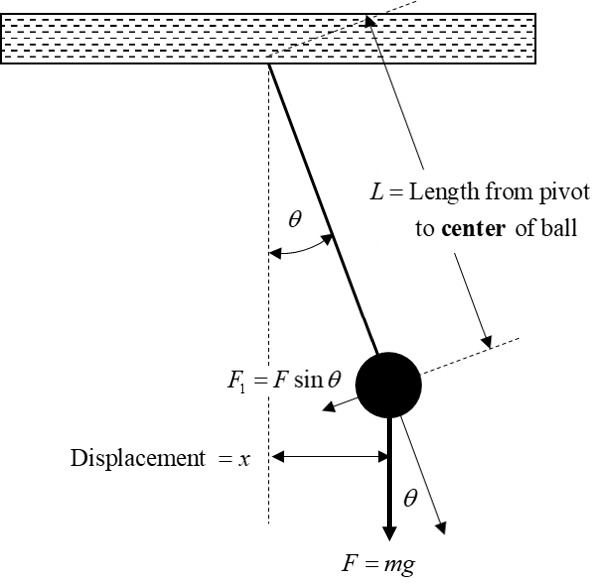
\includegraphics[width=4.0in]{Fall/Experiment03Figures/M10_figure1_squish_v01.png}
  \end{center}
  \caption{Force Diagram and variables used in Experiment M-\ref{lab:M3}.}
  \label{M03Fig01} % Goes AFTER caption
\end{figure}

$F_{1}$, the force along the direction of motion, is equal to $F \sin(\theta) = m g \sin(\theta)$.  We will now make a further simplifying assumption which is to assume that the maximum angular displacement, i.e.\ the maximum value of $x$ is small.  If the value of $x$ and therefore $\theta$ is small, then the magnitude of both the $\sin(\theta)$ and $\tan(\theta)$ are essentially equal to $\theta$, measured in radians.  For small angles then, the value of the $\sin(\theta) = x/L$.  The implication of this assumption is that the pendulum never swings very far from the vertical.  Therefore the restoring force, i.e.\ the force that is acting to return the pendulum to its equilibrium vertical position, is assumed to be acting horizontally.  This is clearly never true except at the equilibrium position where the restoring force is zero.  The implication of this assumption is that the actual restoring force is always less than the value we assume it to be.

The period of the pendulum is the time it takes to swing through a complete cycle, or one complete swing back to the starting point.  Using the small angle assumption described above, we can write the restoring force as
\[
	F = -m g \sin(\theta) = -m g \frac{x}{L}.
\]
The minus sign means that the restoring force is in the opposite direction from the displacement $x$.  When the restoring force of a system is of the form $F = -k x$, the system will oscillate in simple harmonic motion.

To see what this motion looks like we will use Newton's Second Law,
\begin{equation}
  \label{eq:M03fma}
  F = -m g \frac{x}{L} = m a
\end{equation}
where $a$ is the acceleration of the mass in the $x$-direction.
Substituting the definition of acceleration
\[
a = \frac{{\rm d}^2 x}{{\rm d} t^{2}}
\]
into Eqn.~\ref{eq:M03fma} yields an equation for displacement, $x$, as a function of time, $t$, namely
\[
-\frac{mg}{L} x(t) = m \frac{{\rm d}^2 x}{{\rm d} t^{2}}.
\]
Upon simplifying, the mass, $m$, disappears, yielding
\[
x(t) = -\left(\frac{L}{g}\right) \frac{{\rm d}^2 x}{{\rm d} t^{2}}.
\]
This second order, linear, differential equation has a solution
\[
x(t) = A \cos\left(2\pi \frac{t}{T} \right)
\]
where $A$, the amplitude, is the maximum value of $x$; $T$ is the period; and the motion is such that at $t = 0$, the pendulum is at its maximum displacement, i.e.\ $x = A$.  Note that the motion is independent of the mass.  Substitution of this solution into the differential equation yields an expression for the period as
\begin{equation}
  \label{eq:M03CalcTime}
  T = 2\pi \sqrt{\frac{L}{g}}.
\end{equation}
Rearranging this expression we obtain
\begin{equation}
  \label{eq:M03Calcg}
  g = 4\pi^2 \frac{L}{T^2}.
\end{equation}

Had we not constrained the motion of the pendulum to small amplitudes, the expression for the period would be given by
\begin{equation}
\label{eq:M03PeriodSeries_pendulum}
T = 2\pi \sqrt{\frac{L}{g}}  \left[ 1 +
  \frac{1}{ 4} \sin^2\left(\frac{\theta}{2}\right) +
  \frac{9}{64} \sin^4\left(\frac{\theta}{2}\right) + \ldots \right]
\end{equation}
Thus as the angle gets larger, the period increases.

When the pendulum swings with very small angles, the period is essentially independent of the amplitude.  However, from the more precise expression above for the period, this is not strictly true.  An amplitude decrease could result from the effects of friction in the pivot or air drag of the thread and mass.  Pendulum clock makers go to great pains to not only keep the length constant, but the amplitude of the swing as well.  Since we will average over many cycles, we must also assume that the amplitude does not change as we measure the period.  In our experiment, we might be tempted to average a very large number of cycles to reduce measurement errors.  However the necessarily larger initial amplitude together with the decreasing amplitude caused by friction effects would change the average period.  For the last case, we will do just that by deliberately start with a large amplitude and observe whether there is an increase in the measured period.

%\subsection{Case 2 Pendulum moving in a circle}
%
%In Case 2 you will explore the period with the pendulum moving in a circle.
%
%The radius of motion in terms of the length and the angle $\theta$ is $R=L\sin \theta$. The ball moves in a horizontal plane.
%Therefore its vertical component of acceleration is zero and the vertical forces must cancel.
%The vertical component of tension equals the weight of the ball, $F_T \cos\theta = M g$.
%
%The ball is in uniform circular motion around a horizontal circle.
%The centripetal force is
%\begin{equation}
%  F_r = F_T \sin\theta = M g \tan\theta = \frac{M v^2}{L \sin\theta}.
%\end{equation}
%Substituting $v= 2\pi L \sin(\theta)/T$ and solving for $g$ gives:
%\begin{equation}
%  \label{eq:M03circle}
%  g = \frac{4\pi^2 L}{T^2}\cos\theta.
%\end{equation}
%
%Using all your results other than Case 6 calculate the average and standard deviation for your experimental values of $g$ as shown in Eqn.~\ref{eq:errorSigmaX}.
%
%How does the difference of your result for Case 6 from your average $g$ compare with the standard deviation?















\section{Experimental Procedure}


\begin{enumerate}
\item \textbf{OVERALL GOALS:}
\begin{itemize}
    \item We study simple harmonic motion of a simple pendulum to derive acceleration due to gravity.
    \item The pendulum is the combination of both the string and the ball. The pendulum length is the distance from the pivot point to the center of mass of the ball (the center where force of gravity is overall acting upon). The total pendulum length can be determined from adding together the thread length $y$ and the ball radius as determined by:
\begin{itemize}
    \item Measuring thread length $y$ from pivot point to the top surface of the ball.
    \item Measuring diameter of the ball with calipers, and determining radius.
\end{itemize}
\end{itemize}


\item \textbf{Five Cases:} For this experiment, you will use thread lengths of approximately 50, 100, 130, and 170~\centi\meter. You don't have to set the lengths to be exactly those lengths. The point here is to cover a wide range to investigate how the motion is dependent on pendulum length. Get close and just make sure to measure the thread length carefully; record the measured value, and determine the total pendulum length for the given case. 
\begin{enumerate}
\item\label{step:M03Case1} $y\simeq  50\,\centi\meter$ with a small angle (displacement from rest of $\sim$1--3\degree, $\sim$1--2 inches, $\sim$1--2 finger knuckles).
%\item\label{step:M03Case2} $y\simeq  50\,\centi\meter$ Leave the length the same as Case~\ref{step:M03Case1} and use a small angle with circular motion.
%  \subitem -Leave the pendulum length the same as Case 1.
%  \subitem -Hold the weight displaced about 2~\centi\meter from its resting place.
%  \subitem -Give it a small initial velocity perpendicular to the displacement to make it move in a circle. Practice a few times to get it to move close to a circle.
\item\label{step:M03Case3} $y\simeq 100\,\centi\meter$ with a small angle.
\item\label{step:M03Case4} $y\simeq 130\,\centi\meter$ with a small angle.
\item\label{step:M03Case5} $y\simeq 170\,\centi\meter$ with a small angle.
\item\label{step:M03Case6} $y\simeq 170\,\centi\meter$ with a large angle.
  \subitem -Do not change the thread length in going from case~\ref{step:M03Case5} to case~\ref{step:M03Case6}.
  \subitem -Use an angle of approximately 45\degree--60\degree (a useful and consistent starting point that provides a large angle is the edge of the table).
\end{enumerate}

\item \textbf{NOTE ON NUMBER OF TRIALS:} For each of the five cases, each person will perform 5 time trials. Everyone can record at roughly the same time, but don't worry if you aren't all timing the exact same swings (i.e. someone starts a half or whole cycle late); just make sure to time a total of 10 cycles for each trial. By everyone taking data for 5 time trials each, a two-person group will end up with 10 total data points, and a three-person group will have 15 total data points for each case, etc.

\item Create a data table for the first case (this table can be copied/pasted for the additional cases):
\begin{itemize}
\item Common data for the entire experiment includes the ball diameter and the accepted $g$.
\item Common data for each case includes:
\begin{itemize}
  \item The case number
  \item The case description
  \item Measured thread length $y$
  \item Calculated pendulum length $L$
  \item Estimated uncertainty in length $\delta L$
  \item Approximate angle of displacement $\theta_\text{displacement}$
\end{itemize}
\item Create enough \textbf{rows} to include all time trials for your group
\item For each case, include \textbf{columns} for
  \begin{itemize}
  \item Measured \textbf{total time} of the 10 swings $t_{10\text{cycles}}$
  \item Estimated uncertainty in total time $\delta t_{10\text{cycles}}$
  \item Period $T$ derived from your measured time
  \item Uncertainty $\delta T$ derived from $\delta t_{10\text{cycles}}$
  \item Derived values for $g$ from small amplitude approximation Eqn.~\ref{eq:M03Calcg}
  \item Derived uncertainty $\delta g$
  \item Derived values for corrected value, $g_\text{corrected}$. Corrected by incorporating the smaller terms of the series in Eqn.~\ref{eq:M03PeriodSeries_pendulum}. Obtained by multiplying by the square of the factor in square brackets.
  \item Include \textbf{additional rows} for:
  \begin{itemize}
    \item $T_\text{avg}$: Average $T$ fromo all trials of the current case
    \item $g_{\text{avg}}$: Average $g$ from all trials of the current case
    \item $\delta g_{\text{avg}}$: Average uncertainty of $g$ from all trials of the current case
    \item $g_\text{corrected,avg}$: Average corrected values of $g$
    \item Difference between $g_{\text{avg}}$ and the accepted $g$
  \end{itemize}

  
%    \subitem For each trials, record the total time, the average period and the calculated value of $g$ from Eqn.~\ref{eq:M03Calcg}.
  %\item Calculate the average and standard deviation of $g$ for the case from the ten trials.
%  \item Calculate the difference $\delta g$ between your average value for the case and the accepted $g$.
%  \item Compare $\delta g$ to the expected error based on the standard deviation for the case.
  \end{itemize}
  
%  \item Compute the average and standard deviation of your measured values of $g$ for each case.

    \end{itemize}




%\item \textbf{DATA TAKING:}
%\begin{itemize}
\item Measure the thread length $y$. Attach one end of the thread to the provided pendulum clamp in such a way that you can accurately measure the distance from the pivot to the top surface of the ball. Set the length of the thread approximately to the value for the case (doesn't have to be exact, we're just going for a range of lengths across the cases).
\item Add the radius of the ball to the thread length to establish the pendulum length $L$. Estimate and note the uncertainty in the pendulum length $\delta L$.
\item Note the approximate angle of displacement $\theta_\text{displacement}$ from rest position:
    \begin{itemize}
        \item For cases~\ref{step:M03Case1} -- ~\ref{step:M03Case5}, the starting displacement should be small (e.g. 4\% of $L$, as described above with the approximate thread lengths).
        \item For case~\ref{step:M03Case6}, use a large angle of approximately 45\degree -- 60\degree~(like the edge of the table described earlier).
    \end{itemize}
\item For each case, perform 5 time trials per person (i.e. 10 or 15 total data points per two- or three-person group as mentioned above) as follows:
  \begin{itemize}
  \item Measure the time $t_{10\text{cycles}}$ for 10 cycles of the pendulum. One cycle is going from the pendulum's initial position, swings out, swings back to its initial position.
    \begin{itemize}
        \item Start and stop the stopwatch at one end of a swing where the velocity is zero. It is better not to start the watch as you release the mass, but rather at a later point where $v = 0$. This will insure that your starting point is a $v = 0$ point rather than not because of an initial velocity given to the ball when you release it. 
        \item Count one cycle as the mass returns to the starting point, i.e. after one complete swing out and back.
        \item Suggestion for counting: Index your counting by starting at 0. Starting the stopwatch at 0 and stopping when you say 10 will give you 10 full cycles.
    \end{itemize}
  \item Estimate your time trial uncertainty $\delta t_{10\text{cycles}}$ based on your reaction time (generally ranging $\sim$0.150 -- 0.300 seconds) and your stopwatch precision. (i.e. results are $t_{10\text{cycles}} \pm \delta t_{10\text{cycles}}$). \textit{CONSIDER}: Where do the uncertainties come from?
  \item Determine the period $T$ for one cycle from each time trial of ten cycles.
  \item Similarly, determine the period uncertainty $\delta T$ for one cycle from each time trial. (Hint: how many cycles did you observe?)
  \item Calculate the value of $g$ for each time trial using the small amplitude approximation, Eqn.~\ref{eq:M03Calcg}.
  \item Similarly, determine the uncertainty of your value for $g$ by making $g$ as large as your uncertainty allows and subtract the original value; the difference is the uncertainty in $g$. In other words, maximize $g_{\text{maximize}}$ with a smaller period and larger pendulum length: using ($T - \delta T$) as the period and ($L + \delta L$) to make $g_{\text{maximize}}$ bigger by dividing by a smaller period and multiplying by a longer length). Then get the uncertainty by $\delta g = g_{\text{maximize}} - g$.
  \subitem \begin{equation}
  \label{eq:M03Calcg_subitem_maximized}
  g_{\text{maximize}} = 4\pi^2 \frac{(L + \delta L)}{(T - \delta T)^2}
\end{equation}
\item Calculate the corrected value, $g_\text{corrected}$, by including the next two terms of the series according to Eqn.~\ref{eq:M03PeriodSeries_pendulum} obtained by multiplying by the square of the factor in square brackets. This is like Eqn.~\ref{eq:M03Calcg} becoming:
  \subitem \begin{equation}
  \label{eq:M03Calcg_subitem_corrected}
  g = 4\pi^2 \frac{L}{T^2} \left[ 1 +
  \frac{1}{ 4} \sin^2\left(\frac{\theta}{2}\right) +
  \frac{9}{64} \sin^4\left(\frac{\theta}{2}\right) \right]^2
\end{equation}
  %\end{itemize}
  \begin{itemize}
  \item Calculate your average values from everyone's trials for the current case:
      \item $T_\text{avg}$, the average value of $T$
      \item $g_{\text{avg}}$, the average value of $g$
      \item $\delta g_{\text{avg}}$, the average uncertainty of $g$
      \item $g_\text{corrected,avg}$, the average corrected value of $g$
  \end{itemize}
  \end{itemize}
  \item Calculate the difference between $g_{\text{avg}}$ and the accepted $g$
%\item Calculate the average and standard deviation of $g$ from the 10 trials.
%\item Calculate the expected error in your average value of $g$ for the case.
%\item Compare this expected error to the difference between the accepted value of $g$ and the average value for the case.
\item Compare your value for $g \pm \delta g$ to the difference between the accepted value of $g$ and the average value for the case. \textit{DISCUSSION POINT}: Do your experimental values for $g$ agree with the accepted value of $g$. In other words, does $g \pm \delta g$ overlap with the accepted value by covering the difference between the experimental and actual values?
%\end{itemize}



%  \item Now analyze the overall results of the experiment. \textbf{For each case} create a row in your data layout that includes:
%  \begin{itemize}
%    \item the average period for the case.
%    \item the average measured value of $g$ using the small amplitude approximation, Eqn.~\ref{eq:M03Calcg}.
%    \item the corrected average measured value of $g$ corrected according to Eqn.~\ref{eq:M03PeriodSeries_pendulum} obtained by multiplying by the square of the factor in square brackets.
  %  \item the standard deviation of the measured value of $g$,
  %  \item the difference between the measured value and the accepted value of $g$,
  %\end{itemize}
%\end{itemize}


\item{\textbf{Graphical Analysis:}}

\begin{itemize}
\item Using data from the four small amplitude cases (Cases~\ref{step:M03Case1}--~\ref{step:M03Case5}), plot the square of the average period, $T^2$, as a function of the length $L$. \textbf{Do not} use the large angle Case~\ref{step:M03Case6}.
\item Plot all data points from your lab group and draw the best fit straight line through your data points (force the fit to pass through the origin).
\item Determine the slope of your graph.
\item From the expression for the period, the measured slope, $m$, should give you your best estimate of the value of $g$.  Since the expression for $T^2$ is given by
  \begin{equation}
    \label{eq:M03slope}
    T^2 = \frac{4\pi^2}{g} L
  \end{equation}
  the slope of your graph, $m = 4\pi^2/g$.  Thus your final value for $g_\text{slope}$ is $4\pi^2/m$.
  
!!!!!!!!!!!!!! Add in actual uncertainty from the slope?

  !!!!!!!!!!!!!! Add in actual uncertainty from the slope?


!!!!!!!!!!!!!! Add in actual uncertainty from the slope?


!!!!!!!!!!!!!! Add in actual uncertainty from the slope?


!!!!!!!!!!!!!! Add in actual uncertainty from the slope?


!!!!!!!!!!!!!! Add in actual uncertainty from the slope?

  \item \textit{Consider}: Assuming similar uncertainty in $g$ from the average $\delta g_{\text{avg}}$, does the slope-derived value of $g_\text{slope}$ agree with the accepted value of $g$ better than average $g_{\text{avg}}$ of any individual small amplitude case?
\end{itemize}

\end{enumerate}










\section{Post-Lab Submission --- Interpretation of Results}

\begin{itemize}
\item Make sure to submit your finalized data table (Excel sheet)
\item What are your experimental values of g, and how do they compare to the accepted value? Do this for:
\begin{itemize}
    \item Case averages of $g_{\text{avg}}$, (i.e. does $g_{\text{avg}} \pm \delta g_{\text{avg}}$ overlap with the accepted value by covering the difference between the experimental and actual values?)
    \item Case averaged of $g_\text{corrected,avg}$ (assuming similar uncertainty)
    \item Slope-derived $g_\text{slope}$ (assuming similar uncertainty)
\end{itemize}
\item Case~\ref{step:M03Case6} (large angle):
\begin{itemize}
    \item How is Case~\ref{step:M03Case6} (large angle) different from the previous four?
    \item How does $g_\text{avg}$ of Case~\ref{step:M03Case6} compare to $g_{\text{avg}}$ of Case~\ref{step:M03Case5} (at the same $L$)? 
    \item How does $g_\text{corrected,avg}$ of Case~\ref{step:M03Case6} compare to $g_{\text{avg}}$ of Case~\ref{step:M03Case5} (at the same $L$)? Do they agree more or less after the consideration of additional terms.
\end{itemize}
\item How do the periods relate to different lengths of pendulum?


%\item Compare the value of $g$ from Case~\ref{step:M03Case6} using Eqn.~\ref{eq:M03Calcg} and compare it to Case~\ref{step:M03Case5}. How does the difference compare to the expected error in your experimental value?
%\item Compare the corrected value of $g$ from Case 6 using Eqn.~\ref{eq:M03PeriodSeries_pendulum} with the value of $g$ from Case~\ref{step:M03Case5}. How does the difference compare to the expected error in your experimental value?
\end{itemize}





%\newpage
%\text{ }



%%experiment 1 vector table

\section{Testing your Understanding}

\begin{enumerate}
  %1
\item Determine the $x$ and $y$ component of the vector
  \begin{align*} %
    \vec{F} = 20.00\,\newton \ @ \ 60\degree
  \end{align*}
  \begin{enumerate}
  \item $F_{x} =  10.00\,\newton$ and $F_{y} = +17.32\,\newton$
  \item $F_{x} =  10.00\,\newton$ and $F_{y} = -17.32\,\newton$
  \item $F_{x} = -10.00\,\newton$ and $F_{y} = +17.32\,\newton$
  \item $F_{x} = -10.00\,\newton$ and $F_{y} = -17.32\,\newton$
  \end{enumerate}
  %2
\item Determine the $x$ and $y$ component of the vector
  \begin{align*} %
    \vec{F} = 20.00\,\newton \ @ \ 120\degree
  \end{align*}
  \begin{enumerate}
  \item $F_{x} =  10.00\,\newton$ and $F_{y} = +17.32\,\newton$
  \item $F_{x} =  10.00\,\newton$ and $F_{y} = -17.32\,\newton$
  \item $F_{x} = -10.00\,\newton$ and $F_{y} = +17.32\,\newton$
  \item $F_{x} = -10.00\,\newton$ and $F_{y} = -17.32\,\newton$
  \end{enumerate}
  %3
\item Consider the two force vectors
  \begin{equation*}
    \begin{aligned} %
      \vec{F}_1 & = 20.00\,\newton \ @ \ 0\degree \\
      \vec{F}_2 & = 20.00\,\newton \ @ \ 90\degree
    \end{aligned}
  \end{equation*}
  The resultant $\vec{R} = \vec{F}_1 + \vec{F}_2$ is
  \begin{enumerate}
  \item $\vec{R} = 20.00\,\newton \ @ \ 45\degree$
  \item $\vec{R} = 20.00\,\newton \ @ \ 225\degree$
  \item $\vec{R} = 28.28\,\newton \ @ \ 45\degree$
  \item $\vec{R} = 28.28\,\newton \ @ \ 225\degree$
  \end{enumerate}
  %4
\item Consider the two force vectors
  \begin{equation*}
    \begin{aligned} %
      \vec{F}_1 & = 20.00\,\newton \ @ \ 0\degree \\
      \vec{F}_2 & = 20.00\,\newton \ @ \ 90\degree
    \end{aligned}
  \end{equation*}
  The force $\vec{F_{3}}$ needed to fulfill the equation $\vec{F}_1 + \vec{F}_2 + \vec{F_{3}} = 0\,\newton$ is
  \begin{enumerate}
  \item $\vec{R} = 20.00\,\newton \ @ \ 45\degree$
  \item $\vec{R} = 20.00\,\newton \ @ \ 225\degree$
  \item $\vec{R} = 28.28\,\newton \ @ \ 45\degree$
  \item $\vec{R} = 28.28\,\newton \ @ \ 225\degree$
  \end{enumerate}
  %5
\item Consider the two force vectors
  \begin{equation*}
    \begin{aligned} %
      \vec{F}_1 & = 28.28\,\newton \ @ \ 45\degree \\
      \vec{F}_2 & = 20.00\,\newton\ @ \ 120\degree
    \end{aligned}
  \end{equation*}
  The resultant $\vec{R} = \vec{F}_1 + \vec{F}_2$ is represented by
  \begin{enumerate}
  \item $R_{x} = +10\,\newton$ and $R_{y} = +37.32\,\newton$
  \item $R_{x} = -10\,\newton$ and $R_{y} = -37.32\,\newton$
  \item $R_{x} = +10\,\newton$ and $R_{y} = +2.68\,\newton$
  \item $R_{x} = +10\,\newton$ and $R_{y} = -2.68\,\newton$
  \end{enumerate}
  %6
\item Consider the two force vectors
  \begin{equation*}
    \begin{aligned} %
      \vec{F}_1 & = 28.28\,\newton \ @ \ 45\degree \\
      \vec{F}_2 & = 20.00\,\newton \ @ \ 120\degree
    \end{aligned}
  \end{equation*}
  The force $\vec{F_{3}}$ needed to fulfill the equation $\vec{F}_1 + \vec{F}_2 + \vec{F_{3}} = 0\,\newton$ is
  \begin{enumerate}
  \item $\vec{F_{3}} = 38.64\,\newton\ @ \ 75\degree$
  \item $\vec{F_{3}} = 38.64\,\newton\ @ \ 225\degree$
  \item $\vec{F_{3}} = 10.35\,\newton\ @ \ 75\degree$
  \item $\vec{F_{3}} = 10.35\,\newton\ @ \ 225\degree$
  \end{enumerate}	
  %6
\item When static equilibrium is reached:
  \begin{enumerate}
  \item the ring is moving with constant, positive velocity.
  \item the ring is moving with constant, negative velocity.
  \item the ring is not moving and is located off-center, nearest the third mass.
  \item the ring is not moving and is located at the center of the force table.
  \end{enumerate}
\end{enumerate}












%experiment 2 acceleration due to gravity from track

\section{Testing your Understanding}

\begin{enumerate}
  %1
\item Assume the following values: $S = 2.20\,\meter$,  $D = 2.00\,\meter$, $H = 22.0\,\milli\meter$, and $t = 6.321\,\second$.  Determine the value of $g$ you would get for these values.
  \begin{enumerate}
  \item $g = 9.70\,\meter\per\second\squared$
  \item $g = 9.76\,\meter\per\second\squared$
  \item $g = 9.81\,\meter\per\second\squared$
  \item $g = 10.0\,\meter\per\second\squared$
  \end{enumerate}
  %2
\item  Assume the following values: $S = 2.20\,\meter$,  $D = 2.00\,\meter$, $H = 22\,\milli\meter$.  Determine the time you would need to measure to get a value of exactly $9.803\,\meter\per\second\squared$.
  \begin{enumerate}
  \item $t = 6.321\,\second$
  \item $t = 6.379\,\second$
  \item $t = 6.386\,\second$
  \item $t = 40.69\,\second$
  \end{enumerate}
  %3
\item Assume the following values: $S = 2.20\,\meter$,  $D = 2.00\,\meter$, $H = 40.0\,\milli\meter$, and $t = 4.747\,\second$.  Determine the value of $g$ you would get for these values.
  \begin{enumerate}
  \item $g = 9.70\,\meter\per\second\squared$
  \item $g = 9.76\,\meter\per\second\squared$
  \item $g = 9.81\,\meter\per\second\squared$
  \item $g = 10.0\,\meter\per\second\squared$
  \end{enumerate}
  %4
\item  Assume the following values: $S = 2.20\,\meter$,  $D = 2.00\,\meter$, $H = 40.0\,\milli\meter$.  Determine the time you would need to measure to get a value of exactly $g = 9.803\,\meter\per\second\squared$.
  \begin{enumerate}
  \item $t = 4.747\,\second$
  \item $t = 4.731\,\second$
  \item $t = 4.736\,\second$
  \item $t = 22.38\,\second$
  \end{enumerate}
  %5
\item  In the measurement of $g$, when determining the starting position of the glider you must:
  \begin{enumerate}
  \item use the same location for all cases, and this location must be directly behind the photogate.
  \item use the same location for all cases, and this location must be underneath the photogate.
  \item use different locations for all cases, and these locations must all be behind the photogate.
  \item use different locations for all cases, and these locations must be between the two photogates.
  \end{enumerate}
\end{enumerate}









%experiment 4 centripetal force

\section{Testing your Understanding}

\begin{enumerate}
  %1
\item A mass $m$ rotates at constant speed $v$ at a radius of $R$ from the rotational axis. A force $F$ provides the centripetal force $F_{c}$. If you double the mass $m$, without changing $R$ or $v$, the force needed to keep the mass in circular motion would
  \begin{enumerate}
  \item stay the same.
  \item double.
  \item halve.
  \item quadruple.
  \end{enumerate}
  %2
\item A mass $m$ rotates at constant speed $v$ at a radius of $R$ from the rotational axis. A force $F$ provides the centripetal force $F_{c}$. If you double the radius $R$ of the motion, without changing $m$ or $v$, the force needed to keep the mass in circular motion would
  \begin{enumerate}
  \item stay the same.
  \item double.
  \item halve.
  \item quadruple.
  \end{enumerate}
  %3
\item A mass $m$ rotates at constant speed $v$ at a radius of $R$ from the rotational axis. A force $F$ provides the centripetal force $F_{c}$. If you double the speed $v$ of the mass, without changing $m$ or $R$, the force needed to keep the mass in circular motion would
  \begin{enumerate}
  \item stay the same.
  \item double.
  \item halve.
  \item quadruple.
  \end{enumerate}
  %4
\item A mass $m$ rotates at constant speed $v$ at a radius of $R$ from the rotational axis. A force $F$ provides the centripetal force $F_{c}$. If you double both, the mass $m$ and the radius $R$ of the motion, without changing $v$, the force needed to keep the mass in circular motion would
  \begin{enumerate}
  \item stay the same.
  \item double.
  \item halve.
  \item quadruple.
  \end{enumerate}
  %5
\item A mass $m$ rotates at constant speed $v$ at a radius of $R$ from the rotational axis. A force $F$ provides the centripetal force $F_{c}$. If you double both, the speed $v$ of the mass and the radius $R$ of the motion, without changing $m$, the force needed to keep the mass in circular motion would
  \begin{enumerate}
  \item stay the same.
  \item double.
  \item halve.
  \item quadruple.
  \end{enumerate}
  %6
\item A mass $m$ rotates at constant speed $v$ at a radius of $R$ from the rotational axis. A force $F$ provides the centripetal force $F_{c}$. If you double $m$, $R$, and $v$, the force needed to keep the mass in circular motion would
  \begin{enumerate}
  \item stay the same.
  \item double.
  \item halve.
  \item quadruple.
  \end{enumerate}
  %7
\item When you change the mass or the radius of the free mass, you make the same change to the fixed mass because
  \begin{enumerate}
  \item the fixed mass and free mass contribute equally to the centripetal force.
  \item the fixed mass contributes less than the free mass to the centripetal force, but it is still important.
  \item the noise in the measurements will be larger due to vibration if the fixed and free masses are not balanced.
  \item the device will not rotate if the fixed and free masses are not balanced.
  \end{enumerate}
\end{enumerate}









%experiment 5 energy conservation

\section{Testing your Understanding}

\begin{enumerate}
  %1
\item Calculate the potential energy of an object with mass $m = 140\,\gram$ at a height $h = 11\,\centi\metre$. Use $g = 9.803\,\metre\per\second\squared$ for the acceleration due to gravity and assume that $U = 0\,\joule$ at $h = 0\,\centi\metre$.
  \begin{enumerate}
  \item $U = 0.151\,\joule$
  \item $U =  15.1\,\joule$
  \item $U =   151\,\joule$
  \item $U = 15100\,\joule$
  \end{enumerate}
  %2
\item Suppose an object at a given location has potential energy of $U_i = 10\,\joule$ and kinetic energy of $K_i = 20\,\joule$. Assuming there are no other outside forces acting on the object, how much kinetic energy does the object have when its potential energy is $U_f = 25\,\joule$.
  \begin{enumerate}
  \item $K_f =  5\,\joule$
  \item $K_f = 20\,\joule$
  \item $K_f = 35\,\joule$
  \item This situation cannot be achieved.
  \end{enumerate}
  %3
\item Suppose an object at a given location has potential energy of $U_i = 10\,\joule$ and kinetic energy of $K_i = 20\,\joule$. Assuming there are no other outside forces acting on the object, how much kinetic energy does the object have when its potential energy is $U_f = 40\,\joule$.
  \begin{enumerate}
  \item $K_f = -10\,\joule$
  \item $K_f =  20\,\joule$
  \item $K_f =  50\,\joule$
  \item This situation cannot be achieved.
  \end{enumerate}
  %4
\item Suppose an object at a given location has potential energy of $U_i = 10\,\joule$ and kinetic energy of $K_i = 20\,\joule$. Assuming there are no other outside forces acting on the object, how much potential energy does the object have when its kinetic energy is $K_f = 15\,\joule$.
  \begin{enumerate}
  \item $U_f =  5\,\joule$
  \item $U_f = 10\,\joule$
  \item $U_f = 15\,\joule$
  \item This situation cannot be achieved.
  \end{enumerate}
  %5
\item Suppose an object at a given location has potential energy of $U_i = 10\,\joule$ and kinetic energy of $K_i = 20\,\joule$. Assuming there are no other outside forces acting on the object, how much potential energy does the object have when its kinetic energy is $K_f = 40\,\joule$.
  \begin{enumerate}
  \item $U_f = -10\,\joule$
  \item $U_f =  10\,\joule$
  \item $U_f =  40\,\joule$
  \item This situation cannot be achieved.
  \end{enumerate}
  %6
\item Suppose an object of mass $m = 4\,\kilo\gram$ is at rest at a given location with potential energy of $U_i = 50\,\joule$. Assuming there are no other outside forces acting on the object, how fast does the object move when it reaches potential energy of $U_f = 0\,\joule$?
  \begin{enumerate}
  \item $v_f =  0\,\meter\per\second$
  \item $v_f =  5\,\meter\per\second$
  \item $v_f = 10\,\meter\per\second$
  \item $v_f = 25\,\meter\per\second$
  \end{enumerate}
  %7
\item You try to release the glider with zero initial velocity just at the point where the timer triggers because
  \begin{enumerate}
  \item if you start it further to the right it travels farther and so takes longer to reach the bottom.
  \item if you start it further to the right it has an initial velocity when it passes the timer.
  \item it doesn't really matter where you start the glider because the distance between the gates is the same.
  \end{enumerate}
\end{enumerate}






%experiment 6 Ballistic Pendulum and projectile motion

\section{Testing your Understanding}

\begin{enumerate}
  %1
\item A projectile of mass $m = 0.2\,\kilo\gram$ and initial speed $v_i = 200\,\meter\per\second$ hits a stationary target of mass $M = 2\,\kilo\gram$ and gets imbedded in it. Immediately after the collision the projectile-target combination has a speed $V$ of
  \begin{enumerate}
  \item $V = 18.2\,\meter\per\second$
  \item $V = 20.0\,\meter\per\second$
  \item $V = 60.3\,\meter\per\second$
  \item $V = 63.2\,\meter\per\second$
  \end{enumerate}
  %2
\item A projectile of mass $m = 0.2\,\kilo\gram$ and initial speed $v_i =200\,\meter\per\second$ hits a stationary target of mass $M = 2\,\kilo\gram$ and gets imbedded in it. The energy lost ($\Delta E$) during this collision is closest to
  \begin{enumerate}
  \item $\Delta E =     0\,\joule$ (no energy is lost)
  \item $\Delta E = -3640\,\joule$
  \item $\Delta E = -3670\,\joule$
  \item $\Delta E = -4000\,\joule$
  \end{enumerate}
  %3
\item A projectile of mass $m = 0.2\,\kilogram$ and initial speed $v_i = 200\,\meter\per\second$ hits a stationary target of mass $M = 2\,\kilogram$ and gets imbedded in it. Assuming that all the kinetic energy after the collision is converted into gravitational potential energy, to what maximum height above the original position will the two masses rise?
  \begin{enumerate}
  \item $h = 16.9\,\metre$
  \item $h = 18.6\,\metre$
  \item $h = 20.4\,\metre$
  \item $h = 22.5\,\metre$
  \end{enumerate}
  %4
\item A cannon fires a projectile perfectly horizontal with initial speed of $v_i = 20\,\meter\per\second$. The cannon is at an initial height of $H = 5\,\meter$. How long is the projectile in the air? For simplicity use $g = 10\,\metre\per\second\squared$.
  \begin{enumerate}
  \item $\Delta t = 1.0\,\second$
  \item $\Delta t = 1.4\,\second$
  \item $\Delta t = 2.0\,\second$
  \item $\Delta t = 4.0\,\second$
  \end{enumerate}
  %5
\item A cannon fires a projectile perfectly horizontal with initial speed of $v_i = 20\,\meter\per\second$. The cannon is at an initial height of $H = 5\,\meter$. At what horizontal distance $R$ from the launch position will the projectile hit the ground? For simplicity use $g = 10\,\meter\per\second\squared$.
  \begin{enumerate}
  \item $R = 20.0\,\meter$
  \item $R = 28.0\,\meter$
  \item $R = 40.0\,\meter$
  \item $R = 80.0\,\meter$
  \end{enumerate}
  %6
\item Suppose you have a cannon that is able to fire a projectile from an initial height $H$ with speed $v_i$. If you launch the projectile at a very slight upward angle, the range $R$ (the horizontal distance the projectile travels) will be
  \begin{enumerate}
  \item Larger as compared to if you launch the projectile horizontally.
  \item Less as compared to if you launch the projectile horizontally.
  \item The same as compared to if you launch the projectile horizontally.
  \item The answer depends on the value of the initial speed $v_i$.
  \end{enumerate}
  %7.
\item If you made only $n = 1$ measurement of rack height, the standard deviation of the measurement would be
  \begin{enumerate}
  \item zero, because there is no difference between the value and the average.
  \item Equal to the measured value.
  \item Undetermined, because you need more measurements to find a standard deviation.
  \item Infinite because the denominator $(n-1)$ is zero.
  \end{enumerate}
\end{enumerate}










%experiment 7 for 1171 Rotational Motion

\section{Testing your Understanding}

\begin{enumerate}
  %1
\item \label{item:M09Q1} Determine the moment of inertia $I$ of the Earth on its path around the Sun. Use the following values:
  \begin{align*} %
    & \text{Mass of the Earth: } M_{\mbox{E}} = 6 \times 10^{24}\,\kilo\gram\\
    & \text{Radius of the Earth's orbit around the Sun: } R_{\mbox{ES}} = 150 \times 10^{6}\,\kilo\gram
  \end{align*}
  \begin{enumerate}
  \item $I = 1.35 \times 10^{41}\,\kilo\gram \usk \meter\squared$
  \item $I = 5.40 \times 10^{46}\,\kilo\gram \usk \meter\squared$
  \item $I = 6.75 \times 10^{46}\,\kilo\gram \usk \meter\squared$
  \item $I = 1.35 \times 10^{47}\,\kilo\gram \usk \meter\squared$
  \end{enumerate}
  %2
\item Consider problem~\ref{item:M09Q1} above. How would the value you found for $I$ change if the Earth's year were only half as long (i.e.\ 182.5 days instead of 365 days)?
  \begin{enumerate}
  \item The value of $I$ would double.
  \item The value of $I$ would be half.
  \item The value of $I$ would not change.
  \item The value of $I$ would quadruple.
  \item The value of $I$ would be one quarter.
  \end{enumerate}
  %3
\item Consider problem~\ref{item:M09Q1} above. How would the value you found for $I$ change if the radius of the Earth's path around the Sun would be only half as large (i.e.\ $75 \times 10^{6}\,\kilo\meter$ instead of $150 \times 10^{6}\,\kilo\meter$)?
  \begin{enumerate}
  \item The value of $I$ would double.
  \item The value of $I$ would be half.
  \item The value of $I$ would not change.
  \item The value of $I$ would quadruple.
  \item The value of $I$ would be one quarter.
  \end{enumerate}
  %4
\item \label{M09Q4} Consider the sketch of the setup for this experiment above. Assume that the tension in the string running over the pulley is $T = 10\,\newton$ and the radius of the pulley is $R = 10\,\centi\meter$. The torque acting on the pulley is
  \begin{enumerate}
  \item   100\,\newton\metre
  \item    10\,\newton\metre
  \item     1\,\newton\metre
  \item   0.1\,\newton\metre
  \item  0.01\,\newton\metre
  \end{enumerate}
  %5
\item Consider problem~\ref{M09Q4} above. Assuming the pulley is a cylindrical, solid disk of mass $M = 5\,\kilo\gram$, the angular acceleration of the pulley is closest to
  \begin{enumerate}
  \item 0.2\,\radian\per\second\squared
  \item 2  \,\radian\per\second\squared
  \item 4  \,\radian\per\second\squared
  \item 20 \,\radian\per\second\squared
  \item 40 \,\radian\per\second\squared
  \end{enumerate}
  %6
\item During a pirouette a figure skater reduces her moment of inertia from $I_1 = 1.24\,\kilo\gram\metre\squared$ to $I_2 = 0.25\,\kilo\gram\metre\squared$ by pulling in her arms. If she rotates with an angular speed of $\omega_1 = 0.5\,\radian\per\second$, before pulling in her arms, what is her final angular speed when she finished the process?
  \begin{enumerate}
  \item  2.48\,\radian\per\second
  \item  0.10\,\radian\per\second
  \item  0.40\,\radian\per\second
  \item  9.92\,\radian\per\second
  \item  0.50\,\radian\per\second
  \end{enumerate}
  %7
\item A solid disk and a thin-walled ring of the same mass and radius roll down an incline, starting from rest and from the same height. Which of these objects will reach the bottom of the incline with a higher speed?
  \begin{enumerate}
  \item The ring.
  \item The disk.
  \item Both will reach the bottom with the same speed.
  \item More information is needed to answer this question.
  \end{enumerate}
  Hint: Think about what physics quantity is responsible for the rotation of the object and remember that both objects have the same mass and radius.
\item When measuring the smaller pulley, the reading on the calipers is:
  \begin{enumerate}
  \item The inside radius of the pulley (where the string is wound).
  \item The outside radius of the pulley.
  \item The inside diameter of the pulley.
  \item The outside diameter of the pulley.
  \end{enumerate}
\end{enumerate}







%experiment 7 for 1145 Ideal Gas Law

\section{Testing your Understanding}

\begin{enumerate}
  %1
\item Show that both sides of the Ideal Gas Law equation have units of energy (Joules).
  %2
\item Consider a fixed amount of an ideal gas undergoing an isothermal process (``iso'' is the greek word for equal and used as a prefix means that the word following it will remain the same, so here ``isothermal'' means ``constant temperature''). Under these conditions doubling the pressure $P$ of the gas will
  \begin{enumerate}
  \item Double the volume
  \item Halve the volume
  \item Not change the volume
  \item More information is needed to answer this question
  \end{enumerate}
  Note: An ideal gas under these conditions will follow Boyle's Law (sometimes also called Mariotte's Law).
  %3
\item Consider a fixed amount of an ideal gas undergoing an isobaric process (``isobaric'' means ``constant pressure''). Under these conditions doubling the temperature $T$ of the gas will
  \begin{enumerate}
  \item Double the volume
  \item Halve the volume
  \item Not change the volume
  \item More information is needed to answer this question
  \end{enumerate}
  Note: An ideal gas under these conditions will follow Gay-Lussac's Law (sometimes also called Charles' Law).
  %4
\item Consider a fixed amount of an ideal gas undergoing an isochoric process (``isochoric'' means ``constant volume''). Under these conditions doubling the temperature T of the gas will
  \begin{enumerate}
  \item Double the pressure
  \item Halve the pressure
  \item Not change the pressure
  \item More information is needed to answer this question
  \end{enumerate}
  %5
\item In the Analysis at Constant Temperature procedure, why do you have to wait for the temperature and pressure to equalize?
  \begin{enumerate}
  \item If the temperature and pressure are changing, the ideal gas law is not obeyed.
  \item It takes time for the system to come to thermal equilibrium.
  \item You must wait for the air to leak out of the apparatus, so the pressure equalizes.
  \end{enumerate}
\end{enumerate}










%experiment 9 Simple Harmonic Motion

\section{Testing your Understanding}

\begin{enumerate}
  %1
\item A mass $m = 0.4\,\kilo\gram$ is attached to a vertical hanging spring, which obeys Hooke's Law. After hanging the weight the spring is stretched from its equilibrium position by $\Delta y_0 = 0.1\,\metre$. The spring constant $k$ of the spring is
  \begin{enumerate}
  \item $k = 0.025\,\newton\per\metre$
  \item $k = 0.25 \,\newton\per\metre$
  \item $k = 4    \,\newton\per\metre$
  \item $k = 40   \,\newton\per\metre$
  \end{enumerate}
  %2
\item A mass $m = 0.4\,\kilo\gram$ is attached to a vertical hanging spring, which obeys Hooke's Law. After hanging the weight the spring is stretched from its equilibrium position by $\Delta y_0 = 0.1\,\meter$. The mass is then extended an additional $\Delta y = 0.1\,\meter$ \underline{downward} and released from rest. The period of this system is
  \begin{enumerate}
  \item $T = 0.010\,\second$
  \item $T = 0.063\,\second$
  \item $T = 0.100\,\second$
  \item $T = 0.628\,\second$
  \end{enumerate}
  %3
\item A mass $m = 0.4\,\kilo\gram$ is attached to a vertical hanging spring, which obeys Hooke's Law. After hanging the weight the spring is stretched from its equilibrium position by $\Delta y_0 = 0.1\,\meter$. The mass is then extended an additional $\Delta y = 0.1\,\meter$ \underline{upward} and released from rest. The period of this system is
  \begin{enumerate}
  \item $T = 0.010\,\second$
  \item $T = 0.063\,\second$
  \item $T = 0.100\,\second$
  \item $T = 0.628\,\second$
  \end{enumerate}
  %4
\item A mass $m = 0.4\,\kilo\gram$ is attached to a vertical hanging spring, which obeys Hooke's Law. After hanging the weight the spring is stretched from its equilibrium position by $\Delta y_0 = 0.1\,\meter$. The mass is then extended an additional $\Delta y = 0.2\,\meter$ \underline{downward} and released from rest. The period of this system is
  \begin{enumerate}
  \item $T = 0.010\,\second$
  \item $T = 0.063\,\second$
  \item $T = 0.100\,\second$
  \item $T = 0.628\,\second$
  \end{enumerate}
  %5
\item A mass $m = 0.4\,\kilo\gram$ is attached to a vertical hanging spring, which obeys Hooke's Law. After hanging the weight the spring is stretched from its equilibrium position by $\Delta y_0 = 0.1\,\meter$. The mass is then extended an additional $\Delta y = 0.2\,\meter$ \underline{upward} and released from rest. The period of this system is
  \begin{enumerate}
  \item $T = 0.010\,\second$
  \item $T = 0.063\,\second$
  \item $T = 0.100\,\second$
  \item $T = 0.628\,\second$
  \end{enumerate}
  %6
\item A mass $m = 0.05\,\kilo\gram$ is attached to a vertical hanging spring, which obeys Hooke's Law ($k = 100\,\newton\per\metre$). The mass is then extended an additional $\Delta y = 0.1\,\meter$ \underline{downward} and released from rest. After 10 oscillations the amplitude is observered to be $\Delta y = 0.02\,\meter$. The energy lost in the system is
  \begin{enumerate}
  \item $\Delta E = 0.18\,\joule$
  \item $\Delta E = 0.48\,\joule$
  \item $\Delta E = 1.0\,\joule$
  \item $\Delta E = 4.0\,\joule$
  \end{enumerate}
  %6
\item When measuring the period of the glider with the sail, why do you stop the glider after 5 cycles?
  \begin{enumerate}
  \item That is enough to measure an accurate period.
  \item The motion of the glider becomes too small after 5 cycles to accurately determine when to stop the stopwatch.
  \item Five cycles is a compromise with enough cycles to accurately measure the period while the amplitude is roughly the same.
  \item The sail increases the period of the glider so much that it would take too long to measure 10 cycles.
  \end{enumerate}
  %7
\item Which part of the glider should you use when determining the position on the track?
  \begin{enumerate}
  \item The front corner.
  \item The back corner.
  \item Consistently either the front or the back corner.
  \item The center of mass.
  \end{enumerate}

\end{enumerate}





%experiment 10 Simple Pendulum Solve for G

\section{Testing your Understanding}

\begin{enumerate}
  %1
\item Using the small-angle approximation, determine the period $T$ for a pendulum of $L = 1.5\,\meter$ and angle $\theta = 3\degree$. Use $g = 9.803\,\meter\per\second\squared$ for the acceleration due to gravity.
  \begin{enumerate}
  \item $T = 0.39\,\second$
  \item $T = 0.96\,\second$
  \item $T = 1.23\,\second$
  \item $T = 2.45\,\second$
  \end{enumerate}
  %2
\item Using the complete solution (equation~\ref{eq:M03PeriodSeries}), determine the period $T$ for a pendulum of $L = 1.5\,\meter$ and angle $\theta = 3\degree$. Use $g = 9.803\,\meter\per\second\squared$ for the acceleration due to gravity.
  \begin{enumerate}
  \item $T =  0.39\,\second$
  \item $T =  0.96\,\second$
  \item $T =  1.23\,\second$
  \item $T =  2.45\,\second$
  \end{enumerate}
  %3
\item Using the small-angle approximation, determine the period $T$ for a pendulum of $L = 1.5\,\meter$ and angle $\theta = 45\degree$. Use $g = 9.803\,\meter\per\second\squared$ for the acceleration due to gravity.
  \begin{enumerate}
  \item $T =  0.39\,\second$
  \item $T =  0.96\,\second$
  \item $T =  1.23\,\second$
  \item $T =  2.45\,\second$
  \end{enumerate}
  %4
\item Using the complete solution (equation~\ref{eq:M03PeriodSeries}), determine the period $T$ for a pendulum of $L = 1.5\,\meter$ and angle $\theta = 45\degree$. Use $g = 9.803\,\meter\per\second\squared$ for the acceleration due to gravity.
  \begin{enumerate}
  \item $T =  0.41\,\second$
  \item $T =  1.00\,\second$
  \item $T =  1.28\,\second$
  \item $T =  2.55\,\second$
  \end{enumerate}
  % 5
\item If you were to perform this experiment in Denver, CO instead of Fairfield U, how would you expect the period $T$ to change? Assume the exact, identical experimental conditions
  \begin{enumerate}
  \item The period $T$ would stay the same.
  \item The period $T$ would increase.
  \item The period $T$ would decrease.
  \end{enumerate}
  % 6
\item When setting the length of the pendulum, it is important that:
  \begin{enumerate}
  \item The length of string from the pivot to the surface of the ball is exactly the stated length for the case.
  \item The length of string from the pivot to the center of the ball is exactly the stated length for the case.
  \item The accurately measure length of the string plus the radius of the ball is used in the calculations.
  \end{enumerate}
\end{enumerate}





% --------------------------------------
% Front matter proper

\sectionsFront

%%%%%%%%%%%%%%%%%%%%
%                                             %
%                 Vernier Calipers            %
%                                             %
%%%%%%%%%%%%%%%%%%%%

\labChapter{}{Vernier Calipers}

The instrument illustrated in Fig.~\ref{VernierFig01} is a set of calipers.  The calipers have jaws $c$ and $d$ for measuring the diameter of a sphere or cylinder, $A$, or the thickness of any object placed between them. The inside diameter of a cavity is measured with jaws $e$ and $f$.  The depth of a hole is measured with the depth gauge, $g$.  The latter, and jaws $f$ and $d$ form part of a slide on which is engraved an auxiliary scale, the \textsl{Vernier scale} $v$. The scale on the fixed part (which carries jaws $c$ and $e$) is called the main scale. Only the metric scales are shown in the drawing, although the instrument have both U.S.\ and metric main and Vernier scales.

\begin{figure}
  \begin{center}
    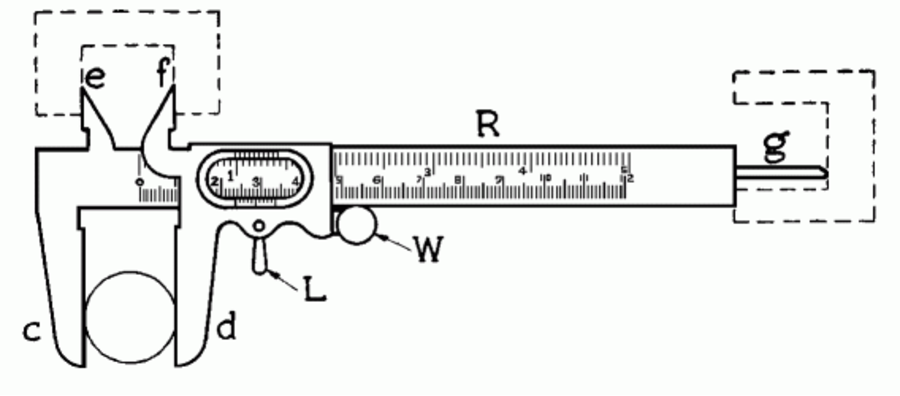
\includegraphics[width=5in]{IntroductionFigures/VernierCalipers01.pdf}
  \end{center}
  \caption{A diagram showing Vernier calipers and their main measurement scales.}
  \label{VernierFig01}  % the \label command comes AFTER the caption
\end{figure}

\section{Reading the Vernier scale}

Vernier scales, as used on the calipers and on many other types of high quality measuring instruments provide a means of reading accurately fractions of a scale division that otherwise have to be estimated.  In Fig.~\ref{VernierFig02}, we have illustrated a main scale with its Vernier scale.

\begin{figure}
  \begin{center}
    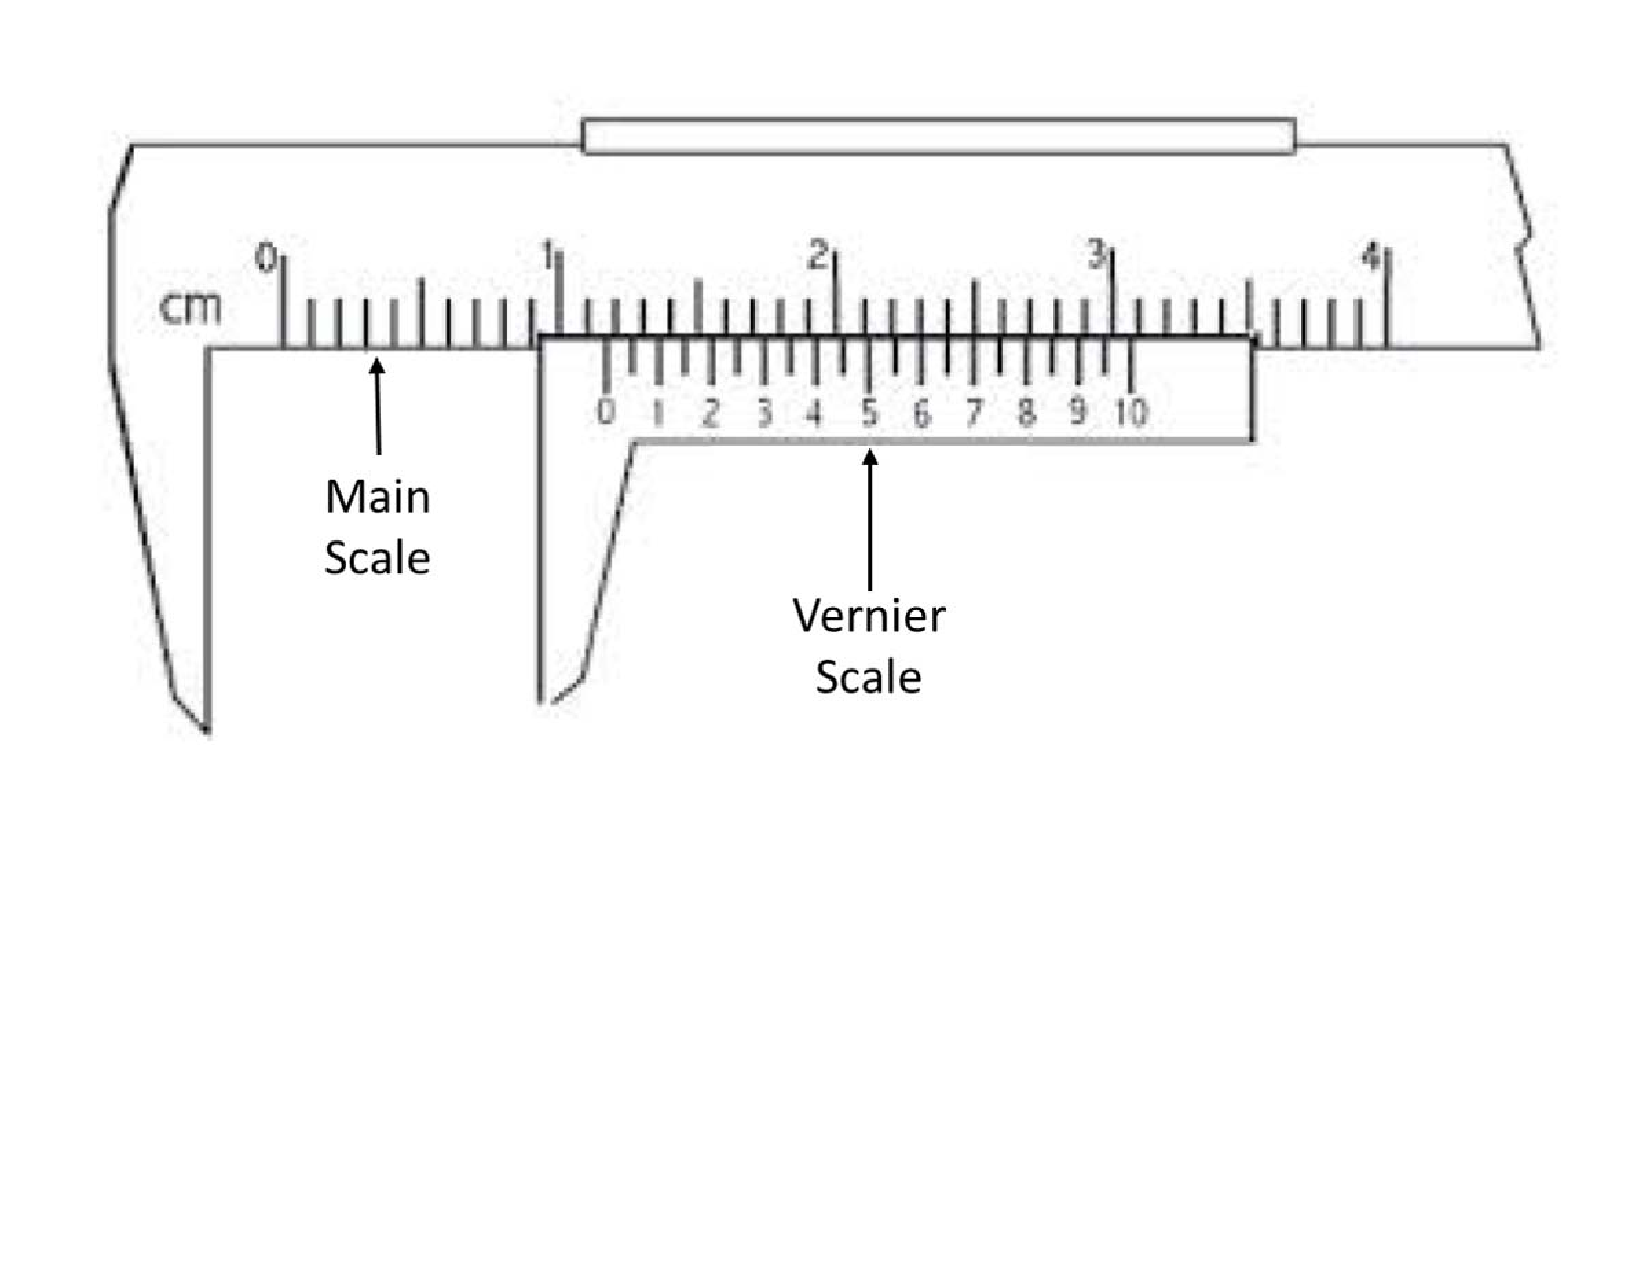
\includegraphics[width=5in]{IntroductionFigures/VernierCalipers02a.pdf}
  \end{center}
  \caption{How to read the value off the caliper slider.}
  \label{VernierFig02}  % the \label command comes AFTER the caption
\end{figure}

If each division on the main scale is $1\,\centi\meter$, then each division of the Vernier scale represents $1.0\,\milli\meter$.  Physically, it is a $9\,\milli\meter$ length divided into 10 equal parts. As an example, in the metric scale of Fig.~\ref{VernierFig02} the zero of the upper or Vernier scale is between the $1$ and $2\,\centi\meter$ marks on the main scale.  In this way, the Vernier scale is capable of interpolating to the nearest \milli\meter, the position of the Vernier zero mark on the main scale.  In this example, the measurement is  $1\,\centi\meter + \mbox{some number of \milli\meter}$.  In order to determine the number of \milli\meter, we read the number on the Vernier scale whose line coincides with a \centi\meter division line on the main scale.  (If the zero line of the Vernier is exactly on a division line of the main scale, then the measurement is exactly the main scale division.)  In this example, the division of the Vernier scale that lines up with a main scale division is the $0.7\,\milli\meter$ division.  The measurement would be $1.17\,\centi\meter$. You might have the situation where there is no exact alignment.  If that occurs, then you would estimate to the nearest $0.5\,\milli\meter$.  For example, if the $7\,\milli\meter$ division was slightly above and the $8\,\milli\meter$ division was slightly below corresponding marks on the main scale, then the measurement would be $1.175\,\centi\meter$.  Thus the Vernier scale is capable of estimating to the nearest $0.05\,\milli\meter$.  The rule for this type of Vernier therefore is to read the number of whole main scale divisions below the zero line of the Vernier, and in the next place of decimals insert the number of the line on the Vernier scale which coincides with a main scale line.

The smallest quantity, which may be read without estimating, is known as the least count; this is $1\,\milli\meter$ for the Vernier calipers illustrated.  For the Vernier calipers you will use in the laboratory, the least count is $0.1\,\milli\meter$.  In general, if the smallest division of the main scale of an instrument is $M$ units, and the length of the smallest Vernier division is $V$ units, then the least count, $L$, is $M V$. Also, since $n$ Vernier divisions are equal in length to $n-1$ main scale divisions,
\[
   nV = (n-1)M
\]
or
\[
   V = \frac{(n-1)M}{n}
\]
and thus
\[
   L = M - V = M - \frac{(n-1)M}{n} = \frac{M}{n}.
\]
         % VernierCalipers
%%%%%%%%%%%%%%%%%%%%
%                                              %
%                 Error Analysis               %
%                                              %
%%%%%%%%%%%%%%%%%%%%

\labChapter{}{Error Analysis}

In laboratory work, it is usually necessary to use experimental apparatus to measure physical quantities. The measurements are seldom, if ever, perfect. As a result, imperfections must be taken into account in any set of physical measurements. One of the most important things to be learned in the laboratory is how to make reliable estimates of the uncertainties involved in any physical measurements and how to handle the propagation of these errors, i.e., to know how the uncertainties affect calculated results of an experiment.


% Types of Errors
\section{Error Analysis Procedure}
\label{sec:ErrorProc}

This section is a guide to performing error analysis for an experiment.  The steps are detailed in the following sections.
\begin{itemize}
\item[\(\triangleright\)] Identify the likely sources of measurement error.
  \begin{itemize}
  \item Measurement errors can stem from the instrumentation, the experimental setup and procedure.
  \item Explain whether errors are systematic or random (\ref{sec:TypesErrors}).
  \end{itemize}
\item[\(\triangleright\)] Estimate the magnitude of the measurement errors using:
  \begin{itemize}
  \item the specification of the equipment,
  \item significant digits displayed,
  \item your estimate of how accurately you can read the instrument,
  \item the range or standard deviation of repeated measurements (\ref{sec:TypesErrors}).
  \end{itemize}
\item[\(\triangleright\)] Calculate the magnitude of the expected error in calculated experimental quantities due to your measurement errors (\ref{sec:ErrorPropagation}).
\item[\(\triangleright\)] If the difference between your results and expected results is much more than the magnitude of error you expect, look for a cause for the difference, including:
  \begin{itemize}
  \item a problem in how the experiment was performed,
  \item a calculation problem, a units conversion error, or using a trig function with degrees instead of radians,
  \item your estimate of the measurement error is too small,
  \item an error in some common value used in the calculations.
  \end{itemize}
\item[\(\triangleright\)] Report your results with the correct number of significant digits (\ref{sec:SigFig}) and with the calculated error.
\end{itemize}

\section{Types of Errors}
\label{sec:TypesErrors}

Experimental measurements are characterized by accuracy and precision. As illustrated in Fig.~\ref{fig:PreciseAccurate}, a set of measurements is precise and accurate if the average value of many measurements is close a known or expected value. A set of measurements is precise if they are closely clustered around their average value. Random errors cause more scatter in the results and reduce the precision of a measurement. Random measurement errors can be due to the inherent limitations of the equipment. They can be estimated and reduced by repeated measurements.  Systematic or precision errors can be due to equipment calibration or approximations in analysis. They reduce the precision of the experiment and are not reduced by repeated measurements. Often you can estimate precision errors by considering the equipment and its specifications.

\begin{figure}%[htbp] %  figure placement: here, top, bottom, or page
  \begin{center}
    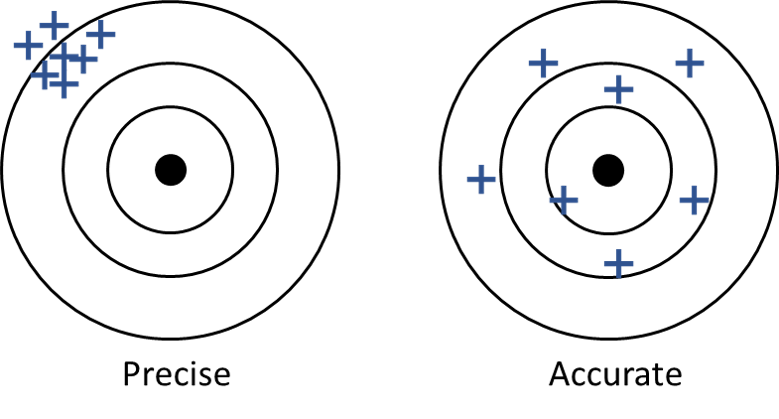
\includegraphics[width=3in]{{IntroductionFigures/ErrorType.png}}
  \end{center}
  \caption{The distinction between precision and accuracy.}
  \label{fig:PreciseAccurate}
\end{figure}

Error analysis can help you recognize if your results are consistent with a known or expected value. Each measurement has some combination of systematic and random errors. Make your best estimate of the possible error in each measured value. Your estimate may include instrument limitations and variation of measurements over multiple trials. Calculate the differences between your experimental results and any known values. Recalculate the experimental value in your spreadsheet by changing your measurements by adding or subtracting the estimated errors. Observe the range of experimental values (maximum and minimum) that you find in these recalculations.  If the expected values fall too far outside this range, there is some problem which you need to address.

Suppose you are measuring the density of a rectangular block. The block has dimensions $L=2.00\,\centi\meter$,  $ W=3.00\,\centi\meter$ and $H=5.00\,\centi\meter$. The mass of the block is $M=60.00\,\gram$. The uncertainty in the length measurements is $\pm0.01\,\centi\meter $ and the uncertainty in the mass is $\pm0.05,\gram$. The calculated density is mass divided by volume. The value calculated directly from your measurements is $\rho_{\mbox{expt}} = \nicefrac{60.00\,\gram}{30.00\,\centi\meter\cubed} = 2.00\,\gram\per\centi\meter\cubed $. The maximum density consistent with your measurements is the ratio of the maximum mass and the minimum volume: \(\rho_{\mbox{max}} = \nicefrac{60.05\,\gram}{\left(1.99\times0.99\times4.99\,\centi\meter\cubed\right)} = 2.02\,\gram\per\centi\meter\cubed\). Similarly, the minimum density consistent with your result is $1.98\,\gram\per\centi\meter\cubed$. If the expected density is not in this range, you need to consider possible explanations: the errors in the measurements could be larger than you estimated, the actual density could be different from the expected value, your calculation may be wrong, or perhaps the shape is not exactly rectangular.

The two types of errors illustrated in Fig.~\ref{fig:PreciseAccurate} require different treatment. The systematic errors illustrated on the target labelled ``Precise'' cannot be reduced by taking more measurements, while the average value obtained with the random errors on the target labelled ``Accurate'' improves with more measurements. The following sections provide guidance on analyzing systematic and random errors.

% Random Errors
\subsection{Random Errors}
\label{sub:RandomErrors}

Random errors are inherent in almost all measurements. They arise because of uncontrollable conditions affecting the observer, the measuring device, and the quantity to be measured. On the basis of probability it is assumed that these errors are as likely to be positive as negative, and more likely to be small than large. Taking a number of independent measurements of a given physical quantity and using the arithmetic average of these values in any computation may therefore minimize their effect. This minimization is only achieved if the measurements are independent. A common mistake is biasing a new measurement to agree with the previous measurements. This mistake makes the measurements more precise, but less accurate as shown in Fig.~\ref{fig:PreciseAccurate}. Taking truly independent measurements is the best way to reduce random error.

%The precision with which a physical quantity has been measured depends upon the spread of the set of measurements about their mean value. If the separate measurements are widely dispersed about the mean, the precision is low.  If the separate measurements are all close, the precision is high. There are many methods of estimating the spread of a set of measurements about the mean value. In general, one usually determines the deviations of the measured values from the mean value and then uses some function of these deviations to represent the spread, and thus the precision of the set of measurements.

The most well established method to quantify the spread of random errors in a measurement is to compute the {\it standard deviation}. Suppose you make $N$ measurements $x_1$, $x_2$, \ldots, $x_N$ of a certain quantity $x$. The average value is
\begin{equation}
  \label{eq:errorMeanX}
  \bar{x}=\frac{x_1 + x_2 + \ldots + x_N}{N}=\frac{1}{N}\sum_{i=1}^N x_{i},
\end{equation}
and the standard deviation of the individual measurements is
\begin{equation}
  \label{eq:errorSigmaX}
  \sigma = \sqrt{\frac{(x_1-\bar{x})^2 + (x_2-\bar{x})^2 + \ldots + (x_N-\bar{x})^2}{N-1}} = \sqrt{\frac{1}{N-1} \sum_{i=1}^{n}\left(x_i-\bar{x}\right)^2}.
\end{equation}
In Excel these operations can be carried out using the functions \texttt{AVERAGE()} and \texttt{STDEV()} or \texttt{STDEV.S()}.

If you perform many measurements, then your estimate of the average value improves. The ``standard deviation of the mean'' for $N$ measurements is
\begin{equation}
  \label{eq:errorSigmaMeanX}
  \sigma_{\mbox{mean}} = \frac{\sigma}{\sqrt{N-1}}.
\end{equation}
Your best estimate of a measurement $x$ is then $\bar{x} \pm \sigma_{\mbox{mean}}$.

For example, suppose that four measurements of a length yield, in centimeters, 7.65, 7.61, 7.66, 7.68.  The mean value is
\[
\bar{x} = \left(7.65 + 7.61 + 7.66 + 7.68\right)/4\,\centi\meter
        = 7.65\,\centi\meter,
\]
and the standard deviation is
\[
\sigma = \sqrt{\frac{(7.65-7.65)^2 + (7.61-7.65)^2 + 
                     (7.66-7.65)^2 + (7.68-7.65)^2}{4-1}\centi\meter\squared}
       = 0.029\,\centi\meter.
\]
The standard deviation of the average value is thus reduced to $ 0.029\,\centi\meter / \sqrt{3} =  0.017\,\centi\meter $ and therefore the best estimate of the length is $\bar{x} =  7.65\,\centi\meter \pm 0.017\,\centi\meter$.

%A simple but effective measure of the spread of indeterminate errors in the measurement of a quantity is the average deviation from the mean. Thus, if a given quantity is measured several times and the mean value of these measurements is computed, then the indeterminate error may be represented by the average difference between the mean value and the measured values without regard to sign. For example, suppose that four measurements of a length yield, in centimeters, 7.65, 7.61, 7.66, 7.68. The mean value is 7.65. The deviations without regard to sign are 0.00, 0.04, 0.01, 0.03. The average deviation from the mean is 0.02. If this average deviation is first subtracted from, and then added to, the mean value, an interval is defined (7.63 to 7.67), which generally brackets about half of the measured values. In this example the measurements 7.65 and 7.66 lie within the interval but 7.61 and 7.68 lie outside the interval. In many cases, it is desirable to extend the interval so as to include almost all the measured values, which can generally be done by using twice the average deviation as a measure of the indeterminate errors. The interval in the above example then becomes $7.65 \pm 0.04$ and includes all the measured values.

Frequently, a set of measurements has to be taken in an experiment under a prescribed condition. It may be difficult to judge exactly when this condition is satisfied. In this case, it may be necessary to vary the physical quantities that produce this condition and to note how much each may be varied without appreciably altering the prescribed condition. This variation may be used to determine the error.

Finally, the measuring devices (meter stick, voltmeter, and so on) are not perfectly accurate even if one could make a precise reading with them. The manufacturer specifies the accuracy in the measuring device; for example, a particular type of voltmeter may be guaranteed to give readings accurate to $\pm 1\%$ of full scale reading. Part of this tolerance is random error that can average out by taking multiple readings. As discussed in the next section, another part of the instrument error is systematic. An ammeter may always read $0.5\%$ high because of the value of a resistor internal to the device.

% Systematic Errors
\subsection{Systematic Errors}
\label{sub:SystematicErrors}

Systematic errors occur in an experiment because of a defective measuring apparatus, faulty methods, or incomplete working equations. They are definite in sign and magnitude and cannot be reduced by taking the average of a number of measurements, because the same error is included in each measurement.
These errors are often more important than the random errors. Calibrating the measuring apparatus, modifying the method, or changing the working equations may reduce them. These procedures are generally described as corrections that are to be made in performing the experiment.
For example, the reading of a Vernier caliper may not be zero when the jaws are in contact. This so-called zero error must be corrected for in using the instrument, i.e., the instrument must be calibrated. Otherwise, all measurements made with the caliper will be in error by a determinate amount, the zero error.

In many experiments time is measured with a stopwatch. Using a stopwatch that does not run at the proper rate would introduce an instrumental systematic error. A watch that ran too fast would cause all times recorded to be too high. A more significant systematic error encountered with a stopwatch is reaction time error. In measuring the time for an air track glider to travel down an incline, the observer may introduce a systematic error due to the reaction time required to stop the watch and a random error due to variation in reaction time. Report this source of error as ``reaction time error.'' The expression ``human error'' is too ambiguous to be useful in describing measurement errors.

%An example of personal systematic error is the tendency to look favorably at the first reading taken and then with suspicion on subsequent readings that differ. Other personal errors can be attributed to eyestrain, fatigue, or the position of the eye relative to a scale. Sloppy alignment of the end of a meterstick or failure to properly zero a balance are personal systematic errors which can be avoided with due diligence.

\subsection{Difference between Experimental Value and Expected Value}
\label{sub:ExperimentExpected}

If the true value of a quantity is known, then the systematic error can be estimated as difference between the result observed (experimental value) and the expected value. It is important to remember that this is an estimate of the systematic error. The difference between your experimental value and the expected value is \textbf{not an estimate of the random experimental error}. To report this difference as a percentage, divide the difference by the true value and multiply by 100\%. In Excel, use percent format instead of multiplying by 100\%.

%\begin{align} %
%        \%-\mbox{difference} = \frac{\mbox{Experimental Value} - \mbox{Actual Value}}{\mbox{Actual Value}} \, 100 \%
%\end{align}

If the true value of a quantity is known, then the difference between the experimental value and the expected value must be compared with the estimated systematic and random errors.  The difference between your experimental value and the expected value is \textbf{not an estimate of the experimental error}. To report this difference as a percentage, divide the difference by the true value and multiply by 100. In Excel, use percent format instead of multiplying by 100.

The percent difference between the experimental value and the expected value is
\[
\frac{\mbox{Experimental Value} - \mbox{Actual Value}}{\mbox{Actual Value}} \times 100\%.
\]
For example, suppose a student measures the value of gravity and finds it to be $9.41\,\meter\per\second\squared$, while the standard value is $9.803\,\meter\per\second\squared$.
The systematic relative difference, expressed as a percentage, is $\nicefrac{-0.39}{9.803} \times 100\% = -4.1\%$.
%The difference is $- 0.40 \meter\per\second\squared$.  It is important to maintain the proper sign of the error.
There is no definite allowable difference between the experimental and expected values in the following experiments. However, all measurements should be made with the greatest care, so as to reduce the error as much as possible.

It should be noted that the percent difference is not an estimate of experimental error. Any measurement has random and systematic errors even if the percent difference happens to be small.  Often, scientists do not know the actual value of the quantity they are measuring and they give their best estimate with error. Comparing the difference of the experimental value and the actual value with your best estimate of the experimental error will help determine if there is a systematic error in your results. If the difference is less than your estimated random error, then the results are consistent with the expected value. Having a zero percent difference could be the result of a lucky cancellation of errors and still just means the results are consistent. If the difference is significantly more than the estimated error, then you can begin to ask why your result is not consistent with the expected value.

% Propagation of Systematic Errors
\section{Propagation of Errors}
\label{sec:ErrorPropagation}

Through indirect measurement, the effect of systematic errors can be followed through the equations used. Two simple examples will be discussed.

% Calculation from a single, direct measurement
\subsection{Calculation from a Single, Direct Measurement}

Consider the volume of a sphere $V$ as calculated from a direct measurement of its diameter, $D$.  We would use
\[
  V = \frac{1}{6} \pi \, D^3
\]
where $\pi = 3.1415926\ldots$.  Suppose the value of $D$ is measured as $3.04\,\centi\meter$ and $V$ computed to be $14.71\,\centi\meter\cubed$. It is later discovered that the value of $D$ has a systematic error $\Delta D = +0.01\,\centi\meter$, (unnecessarily large, in all probability). What is the error $\Delta V$ in $V$ and the correct value of $V$?

\begin{enumerate}
\item Direct, brute-force method:\\
  Correct $D$ to $3.03\,\centi\meter$; re-compute $V_{\mbox{corr}}$ as $14.56\,\centi\meter\cubed$.\\
  The systematic error $\Delta V$ in $V$ is then $V - V_{\mbox{corr}} = 0.15\,\centi\meter\cubed$ or +1\%
\item Method based on calculus:\\
  Find the derivative of $V$ with respect to $D$,
  \begin{equation}
    \label{Eq:errorCalcMethod}
    \begin{aligned} %
      \frac{{\rm d}V}{{\rm d}D} &= \frac{3}{6} \pi D^2\\
           {\rm d}V             &= \frac{3}{6} \pi D^2 {\rm d}D.
    \end{aligned}
  \end{equation}
  Note that this shows a direct dependence of a change in $V$ on an infinitesimal change in $D$. Now divide through by $V = \frac{1}{6} \pi \, D^3$
  \[
    \frac{{\rm d}\,V}{V} = 3 \, \frac{{\rm d}\, D}{D}.
  \]
  If a finite change in $D$, such as the systematic error $\Delta D$, is small compared to $D$, then ${\rm d}\,V$ and ${\rm d}\,D$ can be approximated by $\Delta V$ and $\Delta D$, respectively, and so the following can be written:
  \[
    \frac{\Delta V}{V} \approx 3 \, \frac{\Delta D}{D}.
  \]
  This means that the fractional or percent error in $V$ is very nearly 3 times as large as that in $D$. Therefore,
  \[
    \frac{\Delta V}{V} \approx + 3 \, \frac{0.01}{3.04} \approx 1 \%.
  \]
  Hence,
  \[
    \Delta V \approx 0.15\,\centi\meter\cubed
  \]
  and
  \[
    V_{\mbox{corr}} = V - \Delta V = 14.56\,\centi\meter\cubed.
  \]
\end{enumerate}

\subsection{Calculation from Two or More Direct Measurements}

Consider the volume $V$ of a right, circular cylinder as calculated from its diameter $D$ and length $L$. For convenience, let $D$ be measured as $2.00\,\centi\meter$  and $L$ as $5.00\,\centi\meter$. Then,
\[
  V = \frac{1}{4} \pi \, L \, D^2 = 15.71\,\centi\meter\cubed.
\]
If $D$ has an error of $+0.01\,\centi\meter$ and $L$ an error of $-0.02\,\centi\meter$, what is the error $\Delta V$ in $V$ and what is the correct value of $V$?
\begin{enumerate}
\item Direct, brute-force method:\\
  To obtain $V_{\mbox{corr}}$, subtract $0.01\,\centi\meter$ from $D = 2.00\,\centi\meter$, add $0.02\,\centi\meter$ to $L = 5.00\,\centi\meter$ and recompute $V_{\mbox{corr}}$ as $15.61\,\centi\meter\cubed$, whereby $\Delta V$ must be $+0.01\,\centi\meter\cubed$.

\item Method based on calculus:\\
  Find the partial derivatives of $V$
  \[
    \frac{\partial V}{\partial L} =\frac{1}{4} \pi \, D^2   \hspace{2 cm}   \frac{\partial V}{\partial d} =\frac{1}{2} \pi \, D \, L
  \]
  \[
    {\rm d}\, V = \frac{\partial V}{\partial L} \, {\rm d}\, L + \frac{\partial V}{\partial D} \, {\rm d}\, D
  \]
  so that
  \[
    \Delta V \approx \frac{\partial V}{\partial L} \, \Delta L + \frac{\partial V}{\partial D} \, \Delta D = \frac{\pi}{4} \, D^2 \, \Delta L + \frac{\pi}{2} \, D \, L \, \Delta D.
  \]
  Now dividing through by $V = \frac{1}{4}\pi \, D^2 \, L$
  \[
    \frac{\Delta V}{V} \approx \frac{\Delta L}{L} + \frac{2 \Delta D}{D}.
  \]
  i.e.\ the fractional (or percent) systematic error in $V$ is very nearly equal to the fractional systematic error in $L$ plus twice the fractional error in $D$.  In our case,
  \[
    \frac{\Delta L}{L} = \frac{-0.02}{5.00} = -0.4 \%
  \]
  and
  \[
    \frac{2\Delta D}{D} = \frac{+0.02}{2.00} = +1.0 \%
  \]
  so that
  \[
    \frac{\Delta V}{V} \approx +0.6 \%.
  \]

  Thus $\Delta V = +0.09\,\centi\meter\cubed $, i.e.\ the systematic error, is  $+0.09\,\centi\meter\cubed$, the correction is $-0.09\,\centi\meter\cubed$ and $V_{\mbox{corr}} = +15.62\,\centi\meter\cubed $.
\end{enumerate}
% Significant Figures

\section{Significant Figures}
\label{sec:SigFig}

The number of digits required to express the result of an experimental measurement, so that it reflects the accuracy with which the measurement was made, are known as significant figures. Thus, the number of significant figures reflects the limitation of the measuring device and/or the experimenter. Whether the calculations are performed by hand or on a computer, the number of significant figures displayed in the final result must reflect the limitations of the experimental measurement. Often, a computer program will, by default, display either too many or too few digits. If too few digits are displayed, you need to adjust the program setting to show more digits.

For example, if the length of a cylinder is measured as $20.64\,\centi\meter$, this quantity is said to be measured to four significant figures.  If written as  $0.0002064\,\kilo\meter$, we still have only four significant figures. The zeros preceding the ``2'' are used only to indicate the position of the decimal point. The zero between the ``2'' and the ``6'' is a significant figure, but the other zeros are not.  If the above measurement is made with a meter stick, the last digit recorded is an estimated figure representing a fractional part of a millimeter division. All recorded data should include the last estimated figure in the result, even though it may be zero. If this measurement had appeared to be exactly $20$, it should have been recorded as $20.00\,\centi\meter$, since lengths can be estimated by means of this instrument, to about $0.01\,\centi\meter$. When the measurement is written as $20\,\centi\meter$ it indicates that the value is known to be somewhere between $19.5\,\centi\meter$ and $20.5\,\centi\meter$, whereas the value is actually known to be between $19.995\,\centi\meter$ and $20.005\,\centi\meter$.  Conversely, retaining too many significant figures implies greater accuracy than the figures actually represent.

When deciding the number of significant figures to retain, the following rules apply:
\begin{itemize}
	\item[\(\triangleright\)] When collecting data, only one estimated figure is retained as a significant figure.
	\item[\(\triangleright\)] In addition and subtraction, do not carry the result beyond the first column that contains an estimated figure. All figures lying to the right of the last column in which all figures are significant should be dropped.
	\item[\(\triangleright\)] In multiplication and division the result should have as many significant figures as the factor with the least number of significant figures.
	%(In some instances, the result should have one more significant figure than the factor with the least number of significant figures. For example, in the equation $8.5 \times 1.48 = 12.6$, if the result is to be as accurate as the least accurate of the factors, three significant figures are needed even though the factor with the least number of significant figures has two.)
	\item[\(\triangleright\)] When dropping figures that are not significant, round to the nearest significant digit.  That is to say, the last figure should be unchanged if the first figure dropped is less than 5.  The last figure retained should be increased by one if the first figure dropped is 5 or greater.
	\item[\(\triangleright\)] While performing intermediate calculations, it is safer to carry one more significant figure than is required in the final result.  You can always fix it when you're done.
\end{itemize}
The following examples help illustrate these rules.

When adding these four numbers
\begin{equation*}
	\begin{aligned} %
		427&.5\\
		28&.03\\
		0&.0654\\
		396&.0\\
		\hline
		851&.6
	\end{aligned}
\end{equation*}
the result is written rounded to the first decimal digit, 851.6, because the first term in the sum is only given to one decimal digit. The sum is expressed to the proper number of significant figures.

In our next example, we will calculate the area of a rectangle. The length is measured as $1.94\,\centi\meter$, and the width as $1.84\,\centi\meter$. A calculator provides the result of $3.5696\,\centi\meter\squared$. This number has five significant figures while each of the factors has three significant figures. Therefore, the result should have three significant figures and is expressed as $3.57\,\centi\meter\squared$.

In Excel, the number of significant figures can be set by formatting the cell to a ``Number'' type with the desired number of decimal places. In addition to being more meaningful, formatting the cells makes the spreadsheet more readable.
           % ErrorAnalysis
%%%%%%%%%%%%%%%%%%%%%%%%%%
%                                                        %
%                Graphical Representation                %
%                                                        %
%%%%%%%%%%%%%%%%%%%%%%%%%%

\labChapter{}{Graphical Representation of Experimental Data}

From an examination of the tabulated values of a number of measurements of related quantities, it is often difficult to grasp the relationships existing between the numbers. A method widely used to discover such relationships is the graphical method, which gives a pictorial view of the results and makes it possible to interpret the data by a quick glance.

% Independent and Dependent Variables
\section{Independent and Dependent Variables}

In any experimental study of cause and effect the aim is to vary just one condition at a time (the cause) and to observe the corresponding values of another quantity (the effect), which is suspected of being related to the first. The existing relationship is most easily interpreted from the graph if the first of these quantities, the independent variable, is plotted on the abscissa scale ($x$-axis), and the dependent variable is plotted on the ordinate scale ($y$-axis). For example,
\[
y = f(x)
\]
means that for each value $x$, the independent variable, there is a corresponding value of $y$, or, $y$ is a function of $x$.

Graphs should have the following features:
\begin{itemize}
\item[$\triangleright$] Axes tick marks and axis labels indicating the numerical scale  of the quantity,
\item[$\triangleright$] Axes titles with the name of the quantity and the units,
\item[$\triangleright$] A descriptive graph title,
\item[$\triangleright$] Points should not be joined by lines and there is no need to label them with the actual values, and
\item[$\triangleright$] If possible, the full scale should be visible and axes should intersect at $(0,0)$.
\end{itemize}
An example of how a graph should look is shown in Fig.~\ref{fig:graph}.

\begin{figure}%[htbp] %  figure placement: here, top, bottom, or page
  \begin{center}
    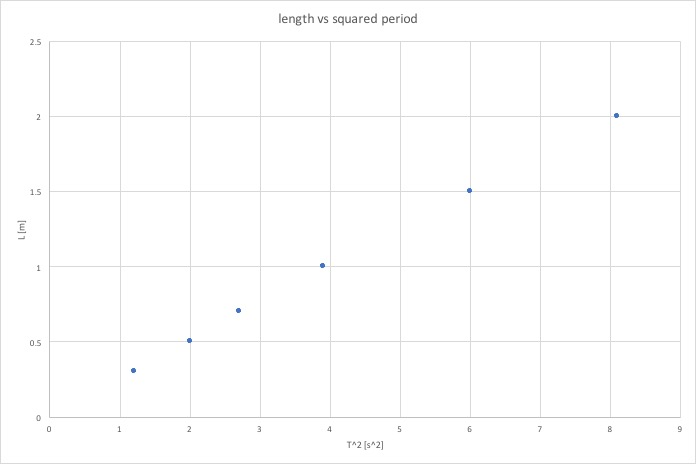
\includegraphics[width=4in]{IntroductionFigures/graph.jpg}
  \end{center}
  \caption{Example of a graph for the pendulum experiment showing the length as a function of the period squared.}
  \label{fig:graph}
\end{figure}

% Producing Graphs
\section{How to Produce Graphs}

There are many ways to produce graphs and just as many computer programs that will aid in the representation of data. This section will give simple instructions on how to make data graphs, using Excel.

\begin{itemize}
\item[$\triangleright$] Using a spreadsheet, it's easiest if you create a separate data table for each graph you want to make. By default Excel expects the first column of the table to be the values for the $x$-axis and the second column the values for the $y$-axis.
\item[$\triangleright$] Highlight \textit{both} columns and select \textbf{Charts} from the toolbar menu. Select the \textbf{Scatter} type and Excel will automatically produce the graph in your spreadsheet.
\item[$\triangleright$] You need to add labels and units to both axes by selecting the option \textbf{Axis Titles} in Excel and then edit the title by clicking on it.
\item[$\triangleright$] Very often you want to add a line-of-best-fit to your Excel graph. To do so follow the steps below:
  \begin{enumerate}
  \item In your graph, right-click (in Windows) or CTRL-click (on Mac) on one of the data points. This will open a pop-up menu. In this menu select \textbf{Add Trendline}. This will open a window with several items related to best-fit-lines and curves.
  \item Select the type of line you would like to add from the \textbf{Type} menu. If you want a straight line select \textbf{Linear}, for a polynomial (e.g.\ a parabola) select \textbf{Polynomial} and then the order will give the highest exponent (for a parabola the order would need to be a \textbf{2}).
  \item In the \textbf{Options} menu you can select two important options for the trend line:
    \begin{itemize}
    \item The \textbf{Set Intercept = \textit{value}} option will force the trendline to go through the point (0,\textit{value}). This is useful if you know that your curve is supposed to go through the origin. In this case set $\mbox{\textit{value}} = 0$ (the default value in Excel) and this forces the best-of-fit-line to go through the origin.
    \item The option \textbf{Display Equation on Chart} will print the equation of the trendline onto the chart. This is useful if you want to determine a value from your line-of-best-fit (e.g.\ the slope). You will have to select the equation and set the format to display the correct number of significant digits. The number of significant digits in an equation displayed on a chart is often too small, and sometimes rounded to 0 if values are small. Select the equation and under the format tab choose Format Selection and select scientific instead of general Alternatively, you can use the Excel functions \texttt{SLOPE()} and \texttt{INTERCEPT()}.  For more sophisticated fitting, the \texttt{LINEST()} function may be of use as well.
    \end{itemize}
  \end{enumerate}
\end{itemize}

Fig.~\ref{fig:graph2} shows again the length as a function of the period squared for a pendulum with a linear trendline. The line is the best fit to the points and the equation shows the resulting slope and intercept. Theoretically the intercept is expected to be zero and the slope is excepted to be $\nicefrac{4\pi^2}{g}=0.248\,\second\squared\per\meter$.  In Excel you can set the equation properties to force the intercept to zero. Often you need to reformat the displayed equation to show enough significant figures.

\begin{figure}%[htbp] %  figure placement: here, top, bottom, or page
  \begin{center}
    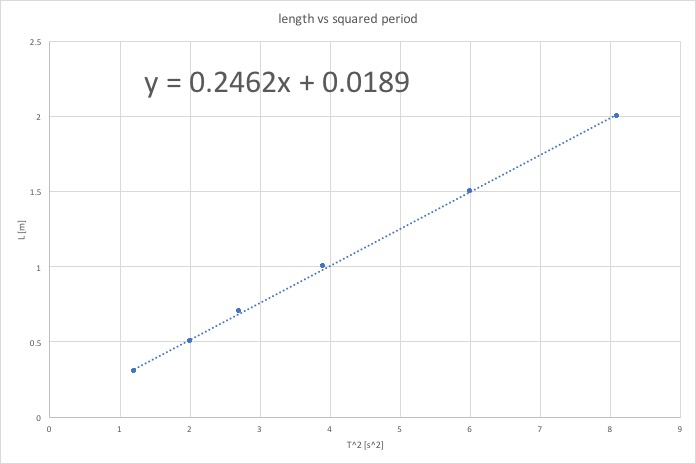
\includegraphics[width=4in]{IntroductionFigures/graph2.jpg}
  \end{center}
  \caption{Example of a graph with the trendline  and the corresponding equation.}
  \label{fig:graph2}
\end{figure}
 % GraphicalRepresentation
%%%%%%%%%%%%%%%%%%%%
%                                                %
%                 Data Acquisition               %
%                                                %
%%%%%%%%%%%%%%%%%%%%

\labChapter{}{Data Acquisition and Analysis}

%% Introduction
%\subsection{Introduction}

In this lab you will perform measurements and calculate results from the measurements. Each trial requires similar calculations.  The best way to perform repetitive calculation tasks is to use a computer program such as a spreadsheet. The effort to set up the calculation is more than compensated by the reliability and ease of repeating calculations. Several experiments will make use of sensors to aid in measurements and data gathering. The data in these experiments is collected by an advanced computer program called \textbf{Capstone}, which is installed on all computers in the lab. The program is also able to organize, analyze, and display the data. This section will give an overview of the program, explain how to set up sensors, and how to display data. More detailed information will be given in the specific experiments, which will make use of the sensors and data acquisition.

\section{Data Analysis with Spreadsheets}
\label{sec:dataSpreadsheet}

Data for each experiment has a set of measurements and calculations.
A spreadsheet is a grid of rows and columns where you can enter text, numerical values or formulas.
Spreadsheet programs provide all the mathematical functions, formatting, and graphing that you need for this lab.
You will often have a table of common values, another for measurements, and a table for summary calculations.
The standard way to structure a data analysis spreadsheet saves calculation errors and reduces repetitive typing.
Use a separate row for each trial and a separate column for each measured or calculated value.

\begin{itemize}
\item[$\triangleright$] Use a row for each trial, labeled in the left cell with, for example, ``Trial \#1''.
\item[$\triangleright$] Use a column for each measured or calculated value, labeled in the top cell with a description of the column and with units.
\item[$\triangleright$] Reference cells you need for a calculation. Do not retype numbers. Use \texttt{\$} for row or column coordinates you don't want to change. \texttt{\$D5} will always refer to column \texttt{D} but the row will change. \texttt{D\$5} will always refer to row 5 but the column will change. Finally, \texttt{\$D\$5} will always refer to the same cell.
\item[$\triangleright$] Never enter a value calculated outside the spreadsheet, for example, on your calculator. Any value you can find on the calculator can be calculated and updated automatically on the spreadsheet.
\item[$\triangleright$] Use the spreadsheet's ``fill down'' capability by selecting a set of cells in a row and fill down by dragging. Formulas will copy and the row numbers of referenced cells that are not preceded by \texttt{\$} will increment automatically.
\end{itemize}
This approach makes it efficient to create a spreadsheet to analyze your data and to correct errors. If you make a mistake in a formula, you can correct the first trial and then correct the other trials by filling down.

\section{Capstone}
\label{sec:SettingUpHardware}

May of our experiments use the \textsl{Capstone} program to
communicate with the measurment hardward and collect the data.  This
section is a very brief introduction to using the \textsl{Capstone}
software. 

% Setting up Hardware
\subsection{Setting up Hardware}

Once you have opened the program you will notice a button labeled \textbf{Hardware Setup} on the left-hand side of the main window. If you click on the button you will get a list of all sensors that are currently connected to the computer. In almost all cases the program will recognize the connected sensor automatically and load a standard setup for the corresponding sensor. In a few cases you will be required to provide the program with certain values needed to determine the value of the quantity the sensor is supposed to measure. In the specific instructions for the experiment you will be told what values to provide. If you do not see the sensor try to dis-  then reconnect the sensor to the computer or ask for help.

% Collecting Data
\subsection{Collecting Data}

Upon opening the \textbf{Capstone} program you have the choice of several display modes for the data you will be collecting. The exact choice depends on the experiment you will be performing and detailed instructions will be provided if they deviate from the description below. In the simplest of all cases you will be using the \textbf{Table \& Graph} display. If you click on this option the program will create a data table and a graph on the main canvas of the program. By default the measurements will be undetermined, but you can choose any variable that is allowed by the sensor to be displayed in the data table columns or on the graph axes. Clicking with the cursor onto the \textbf{Select Measurement} in the data table headers or on graph axes will allow you to chose the variable to display. At times a mathematical equation using the actual measured quantities can be defined by selecting the \textbf{Create New} \(\rightarrow\) \textbf{Calculation} (data table) or \textbf{Add Similar Measurement} (graph axes) option in the pulldown menus.

To start collecting data you need to press the red \textbf{Record} button on the bottom of the \textbf{Capstone} window. The program will then record all data being collected by the sensors and display them as numbers in the data table and points on the graph. The data collection can be stopped by pressing the red \textbf{Record} button a second time. After collecting all the data the information can then be analyzed.

% Analyzing Data
\subsection{Analyzing Data}

Data can be analyzed by exporting the collected data into a data file, that can be read by  Excel (or other mathematical program). An easier way to analyze the data is often to interpret the graph that has been produced by the \textbf{Capstone} program. Tools to analyze the graph are very readily available in the menubar above the graph window. The most important tools are discussed in more detail below:
\begin{itemize}
\item[\(\triangleright\)] \textbf{Highlight range of points in active data}.\\
This option allows you to consider only the highlighted region of the data set to be analyzed. Once selected the program will display a rectangular area that can be resized and dragged over the collected data points. Only the points inside the rectangle will be considered in the selected analysis tool. The selected points will also be displayed in the data table with the same highlighting.
\item[\(\triangleright\)] \textbf{Display selected statistics for active data}.\\
Selecting this option will display several useful mathematical quantities for the selected data set, e.g.\ average of all values, mean of all values, maximum value, minimum value, etc.
\item[\(\triangleright\)] \textbf{Display area under active data}.\\
This option will allow you to calculate the area under the curve for the selected data points (the integral).
\item[\(\triangleright\)] \textbf{Apply selected curve fits to active data}.\\
With this option the user can fit a line of best fit to the elected data range. The drop down menu will give several options for graphs to fit (e.g.\ straight line, parabola, etc.)
\item[\(\triangleright\)] \textbf{Show coordinates and access delta tool}.\\
Once selected this tool will display a cross-hair onto the coordinate frame and allow to determine the values of specific points by placing the cursor onto a data point of the graph. Right-clicking on the cursor will allow to select a delta tool to determine a range in the data set (both $x$- and $y$-range).
\end{itemize}
         % DataAcquisition

% Lab data tables are now a separate document
\end{document}
